% Define colors
\definecolor{keywordcolor}{RGB}{255,0,0}
\definecolor{Classcolor}{RGB}{90, 90, 90}
\definecolor{Funcolor}{RGB}{191, 64, 191}
\definecolor{Logiccolor}{RGB}{51, 179, 255}
\definecolor{commentcolor}{RGB}{0,128,0}
\definecolor{stringcolor}{RGB}{163,21,21}

\renewcommand\lstlistingname{Codeabschnitt}

% Language definition
\lstdefinelanguage{CS}{
    language=C,
    morekeywords=
        {using, public, private, class, yield, return, new, if, else, out, try, catch, for, while, throw, foreach, in, using},
    morekeywords=[2]
        {ARRaycastManager, ARPlaneManager, GameObject, InventoryController, Vector3, ARPlane, Ray, RaycastHit, GetComponent, MeshRenderer, Quaternion},
    morekeywords=[3]
        {Start, Update, Awake, DelayedStart, IsPointerOverPlane, GetCurrentPlaneUnderGaze, SetPlaneColor, PlaceObjectOnDesk, ScreenPointToRay, SetActive, Euler, SetInventoryObject, Raycast},
    morekeywords=[4]
        {+, -, /, *, !, =, 0, 1, 2, 3, 4, 5, 6, 7, 8, 9, null, true, false}, % Define symbols as keywords
    morecomment=[l]{//},
    morecomment=[s]{/*}{*/},
    morestring=[b]",
    sensitive=true
}

\lstdefinelanguage{JavaScript}{
    morekeywords={async, await, break, case, catch, class, const, continue, debugger, default, delete, do, else, export, extends, finally, for, function, if, import, in, instanceof, let, new, return, super, switch, this, throw, try, typeof, var, void, while, with, yield},
    morecomment=[l]{//},
    morecomment=[s]{/*}{*/},
    morestring=[b]',
    morestring=[b]"
}

% Listings settings
\lstset{
    language=CS,
    basicstyle=\footnotesize\ttfamily,
    keywordstyle=\color{keywordcolor}\bfseries,
    keywordstyle=[2]\color{Classcolor},
    keywordstyle=[3]\color{Funcolor},
    keywordstyle=[4]\color{Logiccolor},
    commentstyle=\color{commentcolor},
    stringstyle=\color{stringcolor},
    showstringspaces=false,
    breaklines=true,
    frame=single,
    numbers=left,
    numberstyle=\tiny\color{gray},
    tabsize=4,
    captionpos=b
}

\chapter{Feinkonzept und Realisierung}

\section{Entwicklungsumgebungen}
\subsection{Visual Studio 2022}
Visual Studio 2022 ist eine integrierte Entwicklungsumgebung (IDE) von Microsoft, die speziell für die Entwicklung von
Softwareanwendungen, Webanwendungen und Desktop-Anwendungen konzipiert ist. Es handelt sich um eine umfangreiche
Entwicklungsumgebung, die von Entwicklern weltweit für eine breite Palette von Anwendungsfällen eingesetzt wird.

\subsection{Unity}
Der Unity-Editor, entwickelt von Unity Technologies, fungiert als umfassende integrierte Entwicklungsumgebung (IDE)
und zentrale Arbeitsumgebung für die Konzeption und Umsetzung von 2D-, 3D-, Augmented Reality (AR) und Virtual Reality
(VR) Anwendungen und Spielen. Als Kernelement der Unity-Plattform spielt der Editor eine entscheidende Rolle in der
Entwicklung von Projekten, die auf Unity-Technologien basieren.

Die Funktionalität des Unity-Editors erstreckt sich über verschiedene Aspekte der Softwareentwicklung, angefangen bei
der visuellen Gestaltung von Szenen und Spielwelten bis hin zur Implementierung komplexer Logik und Interaktionen. Die
folgenden Abschnitte vertiefen die Schlüsselmerkmale und Funktionen des Unity-Editors, die ihn zu einem essenziellen
Werkzeug für Entwickler machen.

\subsubsection{Multidisziplinäre Unterstützung und Integration}
Der Unity-Editor zeichnet sich durch seine multidisziplinäre Unterstützung aus, die Entwicklern ermöglicht, kollaborativ
an Projekten zu arbeiten. Künstler, Entwickler und Designer können innerhalb derselben Umgebung zusammenarbeiten,
wodurch ein nahtloser Austausch von Assets, Szenen und Ressourcen ermöglicht wird. Die Integration von Grafik-,
Physik- und Audio-Engines erleichtert die Schaffung immersiver und ansprechender digitaler Umgebungen.

\subsubsection{Szenengestaltung und Asset-Management}
Ein zentrales Merkmal des Unity-Editors ist die intuitive Szenengestaltung, die es Entwicklern ermöglicht,
2D- und 3D-Szenen durch Drag-and-Drop-Operationen zu erstellen und anzupassen. Das Asset-Management ermöglicht eine
effiziente Organisation von Ressourcen wie Modelle, Texturen und Audio-Dateien. Hierbei kommt dem Editor eine
Schlüsselrolle in der Strukturierung und Verwaltung umfangreicher Projekte zu.

\subsubsection{Programmierung und Skripterstellung}
Der Unity-Editor integriert leistungsstarke Programmierfunktionen, die Entwicklern erlauben, Skripte in C-Sharp oder
JavaScript zu verfassen. Die Implementierung von Logik, Interaktionen und Funktionalitäten erfolgt durch die
Integration von Skripten in GameObjects und Szenen. Die Echtzeitansicht von Codeänderungen unterstützt einen
iterativen Entwicklungsprozess.

\subsubsection{Unterstützung für Augmented Reality (AR) und Virtual Reality (VR)}
Der Unity-Editor ist essenziell für die Entwicklung von AR- und VR-Anwendungen. Durch die Integration von AR Foundation
und XR Interaction Toolkit bietet der Editor leistungsstarke Werkzeuge zur Erstellung immersiver Erlebnisse. Die
Möglichkeit, Szenen in Echtzeit in AR- und VR-Geräten zu überprüfen, unterstützt Entwickler bei der Feinabstimmung
und Optimierung ihrer Projekte.

\subsubsection{Erweiterte Debugging- und Profiling-Werkzeuge}
Der Unity-Editor stellt umfassende Debugging- und Profiling-Werkzeuge zur Verfügung, um die Leistung und Funktionalität
von Anwendungen zu optimieren. Durch Echtzeit-Inspektion, Fehlerverfolgung und Ressourcenüberwachung unterstützt der
Editor Entwickler bei der Identifizierung und Behebung von Problemen, um eine reibungslose Ausführung der Anwendungen
sicherzustellen.

\subsubsection{Aufbau einer Unity-Applikation}
Die Struktur einer Unity-Applikation ist entscheidend für eine effektive Entwicklung und Organisation von 3D-Anwendungen
und Spielen. Eine typische Unity-Anwendung besteht aus verschiedenen Schlüsselelementen, darunter Szenen, GameObjects,
Komponenten, Skripte und Assets. Diese werden koordiniert durch die Hauptkomponente der Anwendung, die sogenannte
"GameManager" oder "MainScene". In diesem Abschnitt werden die grundlegenden Bausteine einer Unity-Anwendung sowie
bewährte Praktiken für die Strukturierung und Verwaltung dieser Elemente beleuchtet.

\subsubsection{\label{sec:Shrek is leben}Lebenszyklusmethoden in Unity}
Die Entwicklung von Augmented Reality (AR)-Applikationen in Unity erfordert ein tiefgreifendes Verständnis der
Lebenszyklusmethoden, die in MonoBehaviour-Klassen implementiert werden können. Diese Methoden regeln den Fluss der
Programmlogik und ermöglichen Entwicklern, spezifische Aktionen zu bestimmten Zeitpunkten im Lebenszyklus einer
Anwendung auszuführen.

\begin{itemize}
    \item \textbf{Awake():} Die \texttt{Awake()}-Methode wird aufgerufen, wenn das Skript erstellt wird. Dies geschieht
    vor anderen Initialisierungsmethoden wie \texttt{Start()}. Sie eignet sich für die Durchführung von
    Initialisierungen, bei denen auf andere Skriptkomponenten oder Ressourcen zugegriffen werden soll. Der Hauptzweck
    besteht darin, die Ressourcen für das Skript vorzubereiten.
    \item \textbf{Start():} Die \texttt{Start()}-Methode wird vor dem ersten Frame aufgerufen und bietet die
    Möglichkeit, Initialisierungsaufgaben durchzuführen. Im Gegensatz zu \texttt{Awake()} garantiert \texttt{Start()}
    die vollständige Initialisierung aller GameObjects in der Szene. Entwickler nutzen diese Methode oft für
    Konfigurationen und Vorbereitungen, die spezifisch für die Startphase der Anwendung sind.
    \item \textbf{Update():} Die \texttt{Update()}-Methode ist von entscheidender Bedeutung, da sie in jedem Frame
    aufgerufen wird. Hier kann kontinuierliche Logik ausgeführt werden, wie etwa die Aktualisierung von Animationen,
    die Verarbeitung von Benutzereingaben oder die Anpassung von Positionen basierend auf der Zeit. Es ist wichtig zu
    beachten, dass \texttt{Update()} häufig aufgerufen wird und daher effizient implementiert werden sollte.
    \item \textbf{LateUpdate():} Ähnlich wie \texttt{Update()}, wird aber nachdem alle \texttt{Update()}-Methoden
    aufgerufen wurden. Dies ist besonders nützlich, wenn Anpassungen oder Berechnungen vorgenommen werden müssen,
    nachdem andere GameObjects und Skripte bereits ihre \texttt{Update()}-Logik abgeschlossen haben. Beispielsweise
    eignet sich \texttt{LateUpdate()} gut für Kamera-Anpassungen, bei denen die Position anderer GameObjects bereits
    aktualisiert wurde.
    \item \textbf{OnEnable() und OnDisable():} Die \texttt{OnEnable()}-Methode wird aufgerufen, wenn ein Skript
    aktiviert wird, während \texttt{OnDisable()} aufgerufen wird, wenn es deaktiviert wird. Diese Methoden bieten
    die Möglichkeit, spezifische Aktionen auszuführen, wenn ein Skript seine Ausführung aufnimmt oder beendet.
    Entwickler können diese nutzen, um Ressourcen zu laden oder freizugeben, Abonnements auf Ereignisse
    einzurichten oder abzubrechen, oder um andere vorbereitende oder aufräumende Maßnahmen durchzuführen.
\end{itemize}

\subsubsection{Unity Szenen}
Unity-Szenen bilden das grundlegende Gerüst für die Gestaltung von Inhalten in der Unity-Entwicklungsumgebung. Sie stellen
Assets dar, die alle oder einen Teil eines Spiels oder einer Anwendung enthalten. Szenen bieten eine strukturierte Möglichkeit,
verschiedene Elemente wie \textit{Umgebungen}, \textit{Charaktere}, \textit{Hindernisse}, \textit{Dekorationen} und
\textit{Benutzeroberflächen} zu organisieren und miteinander zu verknüpfen.

Ein wichtiger Aspekt von Unity-Szenen ist ihre Flexibilität. In einem Projekt können \textit{beliebig viele} Szenen erstellt werden,
um die Organisation und Entwicklung des Spiels zu erleichtern. Durch das modulare Konzept von Szenen können Entwickler
einzelne Teile des Spiels separat \textit{bearbeiten} und \textit{optimieren}, was die Zusammenarbeit im Team und die
Wartung des Projekts vereinfacht.

Unity-Szenen dienen nicht nur der Darstellung von Inhalten, sondern auch der \textit{Steuerung} des Spielablaufs. Durch die gezielte
Aktivierung und Deaktivierung von Szenen können verschiedene Abschnitte des Spiels geladen und entladen werden, was die
Leistung und Ressourcennutzung optimiert.

Insgesamt bieten Unity-Szenen eine leistungsstarke und flexible Möglichkeit, Spiele und Anwendungen zu \textit{strukturieren}, zu
\textit{organisieren} und zu \textit{verwalten}. Sie bilden das Grundgerüst für die Entwicklung von Inhalten in Unity und ermöglichen es
Entwicklern, ihre Visionen zu verwirklichen und ansprechende Spielerlebnisse zu schaffen.\footnote{Unity Dokumentation \cite{Scenes}}

\subsubsection{Unity Manager}
Die präzise und immersive Umsetzung von Augmented-Reality-(AR-)Applikationen erfordert den Einsatz spezialisierter Manager,
die grundlegende Funktionen bereitstellen, die für die erfolgreiche Umsetzung verschiedener Szenarien unerlässlich sind.
In dieser Applikation werden zwei Manager aus der breiten Palette von Unity bereitgestellten Managern verwendet. Diese
sind die folgenden:
\begin{itemize}
    \item \textbf{ARPlaneManager\footnote{Unity Dokumentation\cite{PlaneManager}}:}
    Der ARPlaneManager ist ein bedeutender Bestandteil von Unity's Augmented Reality (AR)-Entwicklungsumgebung. Als Teil
    des Unity-eigenen \textit{Mixed Reality Toolkit 3} bietet der ARPlaneManager essenzielle Funktionen zur nahtlosen
    Integration von AR-Elementen in die reale Umgebung. Seine Hauptaufgaben umfassen die automatische Erkennung von
    \textit{horizontalen} und \textit{vertikalen} Flächen in der Umgebung des Benutzers, was die \textit{präzise Platzierung}
    virtueller Objekte auf diesen Flächen ermöglicht. Diese Flächen können verschiedene Strukturen wie \textit{Böden},
    \textit{Tische} oder andere \textit{flache Oberflächen} umfassen. Nach der Erkennung \textit{überwacht} der ARPlaneManager
    \textit{kontinuierlich} die Bewegungen der Flächen in Echtzeit, was essenziell ist, um die \textit{Stabilität}
    virtueller Inhalte auf den realen Flächen zu gewährleisten. Erkannte Flächen können durch \textit{Texturmarkierungen}
    visuell hervorgehoben werden, um dem Benutzer die Grenzen dieser Flächen deutlicher zu zeigen und die Integration von
    virtuellen Objekten zu verbessern. Zudem erleichtert der ARPlaneManager das Platzieren virtueller 3D-Objekte in der
    realen Welt, indem er eine Referenz für die Position und Ausrichtung der erkannten Flächen bereitstellt.

    \item \textbf{ARRaycastManager\footnote{Unity Dokumentation\cite{RaycastManager}}:}
    Der ARRaycastManager in Unity ist eine wichtige Komponente für die Entwicklung von Augmented Reality (AR)-Anwendungen.
    Er ermöglicht es, \textit{Raycasts} von einem \textit{festgelegten Ursprungspunkt} aus durchzuführen, um \textit{Kollisionen}
    oder \textit{Treffer} mit Objekten in der AR-Umgebung zu erkennen. Diese Funktionalität ist entscheidend für die
    genaue Platzierung virtueller 3D-Objekte in der realen Welt, basierend auf den Interaktionen des Benutzers. Der
    ARRaycastManager bietet somit eine grundlegende Funktionalität zur nahtlosen Integration von virtuellen Elementen
    in die physische Umgebung.
\end{itemize}
Die erfolgreiche Umstzung der funktionalen Anforderungen in den spezifischen Augmented-Reality-(AR)-Anwendungsszenarien
des \textit{Knapsack Problems} sowie des \textit{Pings} hängt maßgäblich von der Integration und Anwendung der zwei
genannten Manager, für die Schaffung einer qualitativ \textit{hochwertigen}, \textit{präzisen} und \textit{immersiven}
Benutzererfahrung.

Im Kontext des \textit{Knapsack Problem} Anwendungsszenarios spielt der ARPlaneManager eine zentrale Rolle. Durch die
Markierung von horizontalen Flächen in der Benutzerumgebung garantiert dieser eine präzise Platzierung des virtuellen
Inventar-Objekts und gewährleistet dadurch eine stabile Integration in die reale Umgebung.

Im Kontext des Anwendungsszenarios des \textit{Ping} spielen beide Manager eine wichtige Rolle. Der ARPlaneManager erkennt
die ARPlanes in der Umgebung und der ARRaycastManager erkennt anhand eines Rays, auf welchem ARPlane das reale Kabel, über
das das Ping-Paket visualisiert wird, liegt.

Insgesamt sind diese Manager wichtige Ressourcen, da sie die technische Umsetzbarkeit und Effektivität von AR-Anwendungen
maßgeblich beeinflussen. Durch ihre integrierte Anwendung wird eine nahtlose Verschmelzung von virtuellen und physischen
Elementen realisiert, was eine immersive und präzise AR-Benutzererfahrung sowohl in dem Knappsack-Problem als auch auf
dem Ping Anwendungsszenarios gewährleistet.

\subsubsection{Unity GameObjects und Komponente}
Die Konzeption und Verwaltung von GameObjects stellt einen essenziellen Bestandteil der Entwicklungsumgebung von Unity dar.
Ein \textit{GameObject} repräsentiert in dieser Umgebung jede \textit{Entität} innerhalb eines \textit{digitalen Szenarios},
sei es ein \textit{Charakter}, eine \textit{Umgebungskomponente} oder ein \textit{Effekt}. Diese grundlegenden Objekte
agieren als \textit{Behälter für Komponenten}, welche die \textit{Funktionalität} und das \textit{Verhalten} definieren.

Im Kontext von Unity bilden GameObjects die grundlegenden Bausteine einer Szene. Sie sind abstrakte Entitäten, die allein
nicht aktiv handeln können, sondern erst durch das \textit{Hinzufügen} von \textit{Komponenten} zu funktionalen Einheiten werden. Die Zuweisung
von \textit{Eigenschaften} und \textit{Verhalten} erfolgt durch das Anbringen spezifischer Komponenten an ein GameObject.
Beispielsweise kann einem GameObject, das das Konzept einer Lichtquelle repräsentiert, eine Lichtkomponente zugewiesen werden.

Komponenten in Unity dienen dazu, die Eigenschaften und das Verhalten von GameObjects zu definieren. Sie können beispielsweise
einer Lichtquelle die Fähigkeit verleihen, Licht zu emittieren, oder einem Charakter die Möglichkeit geben, sich zu bewegen
und mit seiner Umgebung zu interagieren. Die Flexibilität von Unity zeigt sich in der Vielfalt der verfügbaren Komponenten,
die sowohl vordefiniert als auch maßgeschneidert sein können. Entwickler können mithilfe der Unity Scripting API eigene
Komponenten erstellen, um spezifische Verhaltensweisen zu implementieren und die Funktionalität ihrer GameObjects zu erweitern.

Insgesamt bilden GameObjects und deren Komponenten das Rückgrat der Entwicklung von Spielen und interaktiven Anwendungen in
Unity. Ihr Verständnis und ihre effektive Verwaltung sind entscheidend für die erfolgreiche Umsetzung digitaler Szenarien
und tragen maßgeblich zur Entwicklung innovativer und ansprechender Spielerlebnisse bei.\footnote{Unity Dokumentation \cite{GameObjects}}.

\subsubsection{Unity Prefabs} \marginpar{\small\(\rightarrow\) HAYLAZ}

Unity bietet mit \textit{Prefabs} eine äußerst praktische Funktion zur Erstellung und Wiederverwendung von Game-Objekten. Prefabs sind modulare, wiederverwendbare Elemente, die als Blaupausen für die Konstruktion von Game-Objekten dienen. Sie ermöglichen Entwicklern, spezifische Objekte oder Objektstrukturen zu erstellen und zu katalogisieren. Diese Muster können dann in unterschiedlichen Szenarien oder Projekten repliziert werden, was eine effiziente Wiederverwendung und Konsistenz über verschiedene Projektumgebungen hinweg ermöglicht.

Prefabs bieten zahlreiche Vorteile für die Gestaltung und Entwicklung von Projekten. Ihr Hauptvorteil liegt in ihrer Fähigkeit, eine effiziente und konsistente Gestaltung von Projekten zu ermöglichen. Sie erleichtern die Wiederverwendung von Designelementen und tragen so zur Effizienz und Konsistenz des Designprozesses bei.

In komplexen Projekten, die eine Vielzahl von Objekten wie Charaktere, Umgebungen und visuelle Effekte beinhalten, erweisen sich Prefabs als äußerst nützlich. Sie dienen als wiederverwendbare Vorlagen, die es ermöglichen, einmal erstellte Elemente zu speichern und in unterschiedlichen Szenarien wiederzuverwenden. Dies eliminiert die Notwendigkeit, jedes Mal, wenn eine neue Szene erstellt werden muss, von Grund auf neu zu beginnen. Darüber hinaus trägt die Verwendung von Prefabs dazu bei, eine konsistente Designästhetik über das gesamte Projekt hinweg zu gewährleisten. \footnote{Unity-Dokumentation, \cite{Prefabs}}\footnote{Unity-Dokumentation, \cite{Prefabs2}}

%TODO: https://docs.unity3d.com/Manual/Prefabs.html
%TODO: https://learn.unity.com/tutorial/prefabs-e#

Ein weiterer bedeutsamer Vorteil von Prefabs besteht in ihrer Fähigkeit, eine unkomplizierte Aktualisierung und Iteration von Projektobjekten zu ermöglichen. Bei notwendigen Modifikationen an einem spezifischen Objekt kann das zugehörige Prefab bearbeitet werden. Diese Modifikationen werden dann automatisch auf alle Instanzen dieses Prefabs angewendet, die in der Szene implementiert sind. Dies optimiert den Workflow und vereinfacht den Prozess erheblich.

Innerhalb des Projekts wird die Prefab-Technologie in folgenden Bereichen eingesetzt:
\begin{itemize}
    \item \textbf{3D-Modelle \ref{sec:3dModelleDustin}:} Die dreidimensionalen Modelle sind als einzelne Prefabs konzipiert. Dies ermöglicht uns, häufige Änderungen am Aussehen der Modelle vorzunehmen, ohne sie einzeln ersetzen zu müssen. Beispiele für die Verwendung dieser Modelle sind QR-Codes, Menü-Objekte und das \textit{Nachrichtenpaket}, welches ein Modell in einem Prefab ist.
    \item \textbf{QR-Codes \ref{sec:qrcodes}:} In unserer Szene arbeiten wir gleichzeitig mit mehreren QR-Codes. Durch die Verwendung der Prefab-Technologie können wir diese mit minimalem Aufwand häufig instanziieren. Auch nach der Instanziierung ist die Arbeit mit diesen virtualisierten QR-Codes vereinfacht.
    \item \textbf{Nachrichteninformationen \ref{sec:pingInfoJonas}:} Im zweiten Anwendungsszenario finden \textit{Prefabs} weiterhin Anwendung. Bei der Versendung von Nachrichten müssen verschiedene Informationen angezeigt werden. Der Zugriff auf diese Informationen ist einfacher, wenn sie in einem Prefab verpackt sind.
\end{itemize}

Zusammenfassend lässt sich sagen, dass Prefabs ein unverzichtbares Werkzeug für die effektive Projektentwicklung in Unity sind. Sie ermöglichen es Entwicklern, Zeit zu sparen, die Konsistenz ihres Projekts zu gewährleisten und den Prozess der Aktualisierung und Iteration von Projektobjekten zu optimieren. Daher sind sie ein wesentlicher Bestandteil jeder effektiven und effizienten Projektentwicklungsumgebung.


\subsection{Deployment der Anwendung} \marginpar{\small\(\rightarrow\) HAYLAZ}

Die Entwicklung unserer Anwendung findet größtenteils auf unseren Laptops statt. Jedoch ist es auf diesen Geräten nur begrenzt möglich, die AR-Funktionalitäten zu testen. Um die Anwendung vollständig auf einem AR-fähigen Gerät zu überprüfen, muss sie auf dieses geladen werden. In diesem Abschnitt wird der genaue Prozess beschrieben, wann und wie die Anwendung auf ein AR-fähiges Gerät deployt wird.

\subsubsection{Voraussetzungen für das Deployment}

Damit das Deployment der Anwendung auf einem AR-fähigen Gerät erfolgreich verläuft, müssen bestimmte Voraussetzungen erfüllt sein:

\begin{itemize}
    \item \textbf{Kompiliertes Unity-Projekt:} Alle erforderlichen Dateien und Ressourcen der Anwendung werden während des Build-Prozesses zu einem ausführbaren Unity-Paket kompiliert.

    \item \textbf{Netzwerkverbindung:} Es ist notwendig, dass sowohl das AR-fähige Gerät als auch der Computer, auf dem der Build durchgeführt wurde, sich im selben Netzwerk befinden. Nur so kann das Unity-Paket über das Netzwerk auf das AR-fähige Gerät übertragen werden.

    \item \textbf{Authentifizierung:} Der Computer, der sich mit der HoloLens verbinden und die Anwendung deployen möchte, muss von der Brille authentifiziert werden. Dies gewährleistet, dass nur autorisierte Geräte Zugriff auf die Brille haben und die Übertragung sicher erfolgt.
\end{itemize}

\subsubsection{Deployment-Prozess}

Die Entwicklung und Bereitstellung einer Anwendung für die HoloLens 2 unter Verwendung von Unity und der Universal Windows Platform (UWP) ist ein strukturierter Prozess, der mehrere Schritte umfasst, beginnend mit der Kompilierung des Unity-Projekts. Dieser Prozess findet auf dem Computer statt, auf dem sich das Unity-Projekt befindet, und kann über das Tastenkürzel \textbf{Strg + Umschalt + B} aufgerufen werden, um die Build-Einstellungen in Unity zu öffnen.

In den Build-Einstellungen wird die Zielplattform festgelegt, auf die die Anwendung bereitgestellt werden soll. Für die HoloLens 2 ist die Universal Windows Platform (UWP) die geeignete Zielplattform aufgrund ihrer Kompatibilität mit diesem Gerät. Die UWP ermöglicht die Entwicklung von Anwendungen, die auf verschiedenen Windows 10/11-Geräten einschließlich der HoloLens 2 ausgeführt werden können.

Es gibt verschiedene Build-Einstellungen, wie in Abbildung \ref{fig:build-settings} dargestellt. Besonders relevant sind dabei die Einstellungen für die \textit{Architektur} und die \textit{Build-Konfiguration}. Die Architektur wird entsprechend der HoloLens 2 auf ARM 64-Bit festgelegt. Die Build-Konfiguration sollte auf \textit{Release} eingestellt sein. Die übrigen Optionen sollten entsprechend den Vorgaben in der Abbildung beibehalten werden. Diese Einstellungen sind wichtig, um in den nächsten Schritten eine funktionierende Übertragung zu garantieren.

\begin{figure}[H]
    \centering
    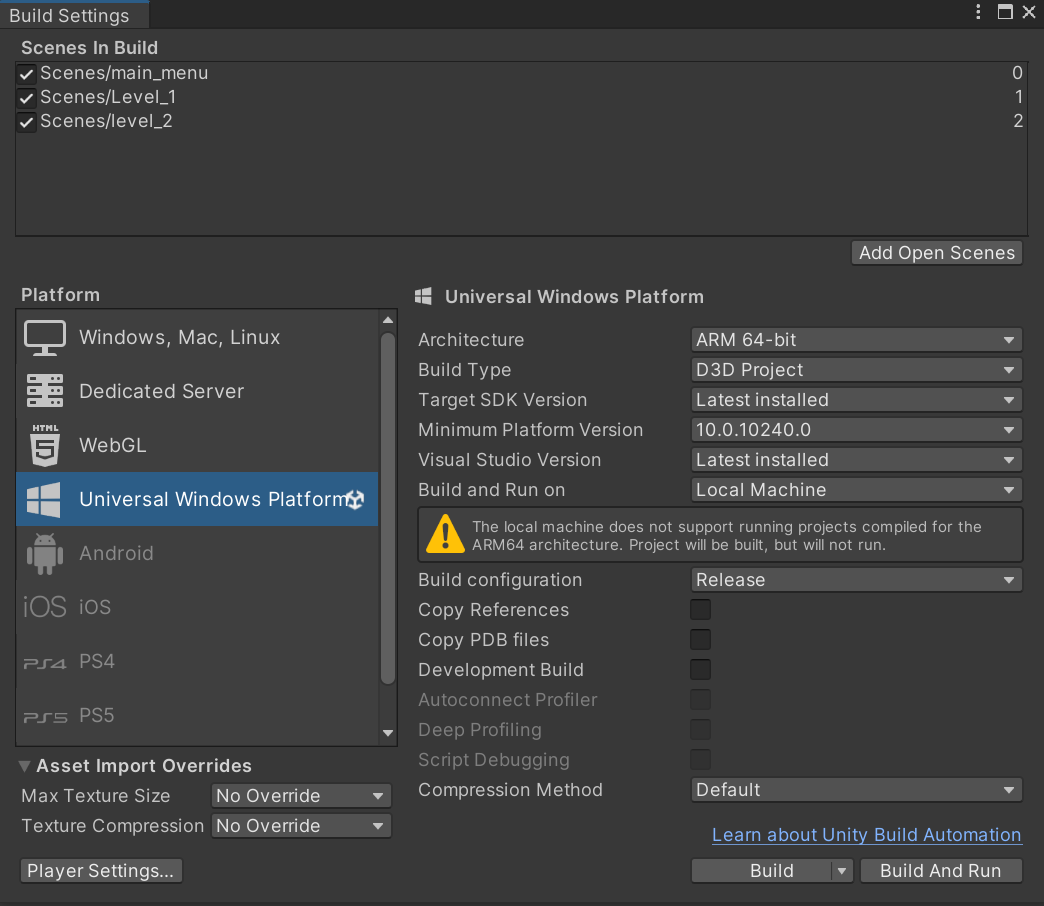
\includegraphics[scale=0.6]{images/build}
    \caption{Build-Einstellungen in Unity}
    \label{fig:build-settings}
\end{figure}

Nach einem erfolgreichen Build erhalten Sie einen Ordner mit den benötigten Dateien für das Deployment. Darin befindet sich unter anderem eine Visual Studio Solution (\textit{VS Solution}), die Informationen zur Struktur des Projekts enthält und Build-Konfigurationen verwaltet. \footnote{Visual Studio Solution, \cite{VS-Solution}}

Der nächste Schritt erfolgt in dieser Visual Studio Solution, in unserem Fall \textit{AARIE.sln}. Nach dem Öffnen der Datei müssen die Konfiguration auf \textit{Release} und die Plattform auf \textit{ARM64} eingestellt werden. Diese zwei Einstellungen sind auf der \textit{Toolbar} zu finden. Außerdem muss die IP-Adresse des AR-fähigen Geräts in den Projekteigenschaften unter Debugging gesetzt werden. Die IP-Adresse der HoloLens 2 kann auf der Brille in den Einstellungen unter Netzwerk gefunden werden. In den Projekteigenschaften ist noch folgende Einstellung zu treffen:

Der Authentication Mode \textit{Universal (Unencrypted Protocol)} wird gewählt, um eine reibungslose Kommunikation zwischen dem Computer und der HoloLens 2 zu ermöglichen, insbesondere während des Deployments der Anwendung. Dieser Modus erlaubt eine unverschlüsselte Kommunikation zwischen den Geräten, was in diesem speziellen Anwendungsszenario aus verschiedenen Gründen vorteilhaft ist. Zum einen vereinfacht die Verwendung eines unverschlüsselten Protokolls die Konfiguration und ermöglicht eine schnellere Einrichtung der Verbindung zwischen dem Entwicklungscomputer und der HoloLens 2. Da dies ein Entwicklungs- und Testumfeld ist, wo Sicherheit weniger prioritär ist als Effizienz und Schnelligkeit, wird diese einfachere Konfiguration bevorzugt. Darüber hinaus minimiert die Verwendung eines unverschlüsselten Protokolls das Risiko von Verbindungsproblemen und -verzögerungen, die bei verschlüsselten Kommunikationsprotokollen auftreten können, insbesondere in lokalen Netzwerken oder Umgebungen, in denen die Infrastruktur möglicherweise nicht optimal konfiguriert ist. In einer Entwicklungs- und Testumgebung, in der die Anwendung iterativ entwickelt und getestet wird, steht die Effizienz im Vordergrund. Die Verwendung eines unverschlüsselten Protokolls erleichtert den Entwicklungsprozess, da sie weniger Overhead und Komplexität mit sich bringt. Es ist jedoch wichtig zu beachten, dass in produktiven Umgebungen, in denen Sicherheit eine höhere Priorität hat, verschlüsselte Kommunikationsprotokolle verwendet werden sollten, um die Vertraulichkeit und Integrität der übertragenen Daten zu gewährleisten. \footnote{Universal Unencrypted Protocol, \cite{VS-Protocol}}

Nachdem alle Einstellungen vorgenommen wurden, kann die

Anwendung auf die HoloLens 2 deployt werden. Dazu muss die Solution mit \textit{Start without Debugging} gestartet werden. Nach einem längeren Ladevorgang wird die Anwendung auf der HoloLens 2 geladen und gestartet.

Falls die Anwendung beendet wird, kann sie auf der HoloLens 2 unter \textit{Start} $\rightarrow$ \textit{Alle Apps} $\rightarrow$ \textit{AARIE} erneut gestartet werden. Falls Änderungen an der Anwendung auf den Computern vorgenommen wurden, muss der gesamte Prozess erneut durchgeführt werden. Es ist wichtig zu beachten, dass die Anwendung nicht automatisch aktualisiert wird.

\subsubsection{Erstmaliges Deployment}
%TODO: MBY ein UML der den Prozess beschreibt?
Beim erstmaligen Deployment auf die HoloLens kann es zu Problemen kommen, die durch die Authentifizierung der HoloLens verursacht werden. In diesem Fall muss der "neue" Computer sich auf der HoloLens erneut authentifizieren. Dazu werden Sie nach dem Starten des Deployments aufgefordert. Auf dem Computer wird ein Authentifizierungscode angezeigt, der auf der HoloLens unter \textit{Einstellungen} $\rightarrow$ \textit{Update \& Sicherheit} $\rightarrow$ \textit{Für Entwickler} $\rightarrow$ \textit{Koppeln} eingegeben wird. Nachdem die Authentifizierung erfolgreich abgeschlossen wurde, kann das Deployment erneut gestartet werden.


\section{Objektdesign} \marginpar{\small\(\rightarrow\) LAMPEL}
Die Bedeutung des Objektdesigns nimmt in der vorliegenden Arbeit einen zentralen Stellenwert ein, wie bereits im Abschnitt \ref{sec:wahlblender} erläutert wurde. Da sämtliche Modelle und Gegenstände eigenständig erstellt werden sollen, ist ein fundiertes Verständnis der grundlegenden Konzepte und Prozesse des Objektdesigns unerlässlich. Im nachfolgenden Abschnitt werden daher alle relevanten Begriffe erläutert, die beim Modellieren auftreten, und die einzelnen Schritte des Modellierungsprozesses werden in möglichst detaillierter Form durchgegangen.

Das Objektdesign umfasst nicht nur die Schaffung von ästhetisch ansprechenden und funktionalen 3D-Modellen, sondern auch die Optimierung dieser Modelle, um ein optimales Benutzererlebnis sicherzustellen. Dies beinhaltet Aspekte wie die Effizienz der Modelle in Bezug auf Rechenleistung und Speicherplatz, die Benutzerfreundlichkeit sowie die visuelle und funktionale Qualität der Modelle.

\subsection{Texturen}
Texturen sind ein wichtiger Bestandteil der Modellierung und verbessern die visuelle Erscheinung von Objekten, um sie realistischer wirken zu lassen. Sie beschreiben die Oberflächenbeschaffenheit eines Objekts, einschließlich Eigenschaften wie Farbe, Rauhigkeit, Reflexionsvermögen, Glanz, Lichtdurchlässigkeit und mehr. In Blender werden Texturen typischerweise als Grafiken oder Muster verwendet, die auf die Oberfläche eines 3D-Modells projiziert werden. Im Projekt wurde viel mit \textit{Bild-Texturen} gearbeitet, um möglichst effiziente, realistische und ästhetisch ansprechende Modelle zu erzeugen.

\subsubsection{Bild-Texturen in der 3D-Modellierung} \label{sec:bildtextures}
Im folgenden Abschnitt wird erläutert, was unter dem Begriff \textbf{Bild-Textur} zu verstehen ist und wie die Umsetzung und Arbeit mit Bild-Texturen im Kontext von Blender funktioniert.

Diese Texturen können als Bilddateien importiert oder innerhalb des Programms selbst erstellt werden.

Die Verwendung von Bild-Texturen ermöglicht es Benutzern, eine Vielzahl von Oberflächeneffekten zu erzeugen, wie beispielsweise Holzmaserungen, Metalltexturen, Stoffmuster und mehr. Durch die Verwendung einer geeigneten Textur kann die visuelle Qualität eines Modells erheblich verbessert werden.

Im Blender-Programm können Bild-Texturen mithilfe des \textit{Shader-Editors} auf das Material des 3D-Objekts angewendet werden. Hierfür wird eine \textit{Image-Texture-Node} erstellt, welche den Farbwert der Textur an das Material übergibt. Es können verschiedene Einstellungen vorgenommen werden, um die Art und Weise der Texturprojektion zu steuern. Zum Beispiel kann die Projektionsart (Box, Flat, Sphere usw.) festgelegt werden, um anzugeben, wie die Textur auf die Oberfläche des Modells angewendet wird. Weitere Einstellungen können die Skalierung der Textur, die Wiederholungsmuster, die Mischmodi und andere Textureigenschaften umfassen. \footnote{Blender \cite{Texturen}}
% https://docs.blender.org/manual/en/latest/render/shader_nodes/textures/image.html

% https://docs.blender.org/manual/en/latest/editors/shader_editor.html
\subsubsection*{Einschub Shader-Editor}
Dieser Editor hat in Blender eine spezielle Funktion. Hier können mithilfe von sogenannten \textit{Nodes} Eigenschaften für Texturen und Materialien vergeben werden. Der Editor wurde im Projekt hauptsächlich für die Anwendung von Bild-Texturen genutzt.

\begin{figure}[H]
    \centering
    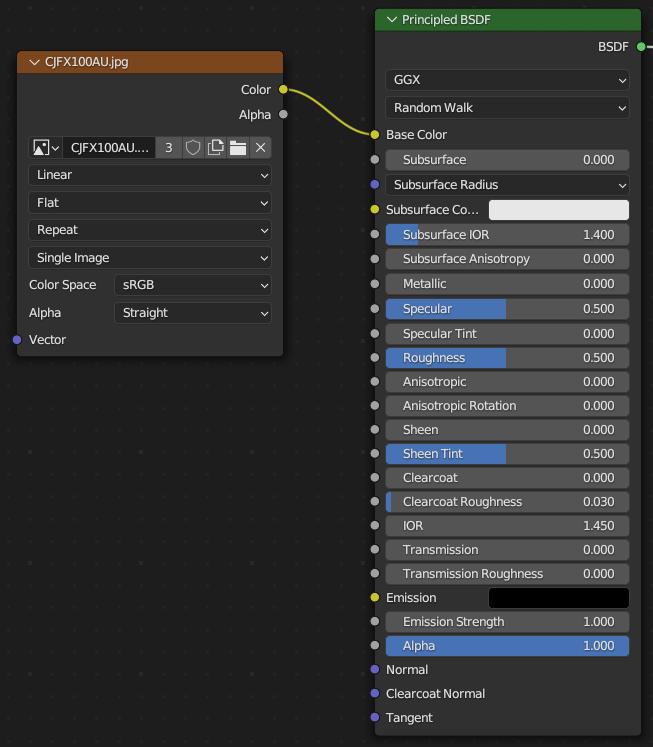
\includegraphics[width=0.6\textwidth]{images/shadereditor.png}
    \caption{Beispielhafte Ansicht auf Bild-Textur-Nodes im Shader-Editor}
    \label{fig:shadereditor}
\end{figure}

In Abbildung \ref{fig:shadereditor} ist zu erkennen, wie die Bild-Textur-Node den Farbwert an das Material weitergibt. Als Beispiel wurde hier der Taschenrechner verwendet, der im Laufe des Kapitels noch näher erläutert wird. Die Abbildung zeigt die verschiedenen Konfigurationsmöglichkeiten, die bereits im Abschnitt \ref{sec:bildtextures} erläutert wurden.

% Die Verwendung von Bild-Texturen in der 3D-Modellierung ist eine wichtige Technik, um realistische und ansprechende Oberflächen zu erstellen, die die visuelle Qualität eines Modells deutlich verbessern können. Durch Anpassung der Textureinstellungen können Benutzer die gewünschten Effekte erzielen und ihre Kreativität bei der Gestaltung von 3D-Modellen ausdrücken.

\subsection{Mesh} \label{sec:mesh}
In der 3D-Grafik bezeichnet ein Mesh eine Sammlung von Eckpunkten, Kanten und Flächen, die die Geometrie eines 3D-Objekts definieren. Es bildet die Grundlage für die Darstellung von Objekten in einer virtuellen Umgebung. Ein Mesh kann aus einer beliebigen Anzahl von Polygonen bestehen, die die äußere Form und Struktur des Objekts definieren.

Die Rolle eines Meshes bei der Modellierung besteht darin, die Form, Oberflächenstruktur und Details eines Objekts zu definieren. Durch die Anordnung und Verbindung der Vertices, Edges und Faces können komplexe geometrische Formen erzeugt werden. Polygone ermöglichen dabei die Darstellung von Objekten mit unterschiedlichen Detailgenauigkeiten. Je mehr Polygone ein Mesh hat, desto detaillierter und realistischer kann das Modell dargestellt werden. Allerdings führt dies auch zu einem höheren Bedarf an Rechenleistung und Speicherplatz.

Meshes werden in verschiedenen Bereichen der 3D-Grafik verwendet, wie zum Beispiel der Modellierung von Objekten, der Animation und der Visualisierung. Sie dienen als Grundlage für die Erstellung von digitalen Szenen.

\subsection{Rolle von Polygonen in einem Modell}
Polygone sind grundlegende Bausteine eines Meshes und spielen eine wichtige Rolle bei der Darstellung von 3D-Modellen. Sie bestehen aus einer Reihe von Eckpunkten (Vertices), Kanten und Flächen, die diese Punkte miteinander verbinden. In einem 3D-Modell definieren Polygone die Form, die Oberflächenstruktur und die Details eines Objekts.
\footnote{CGIFurniture \cite{What are Polygons}}
%https://cgifurniture.com/what-are-polygons-in-3d-modeling/

Durch die Anordnung und Verbindung von Polygonen entstehen komplexe Strukturen, die eine visuelle Darstellung von Objekten ermöglichen. Je mehr Polygone ein Modell hat, desto detaillierter und realistischer kann es dargestellt werden. Allerdings führt dies auch zu einem höheren Bedarf an Rechenleistung und Speicherplatz. Polygone sind somit ein wesentlicher Bestandteil eines Meshes und tragen maßgeblich zur visuellen Qualität und Komplexität eines 3D-Modells bei.

\subsection{Optimierung der einzelnen Modelle}
Der Entwurf von 3D-Objekten mit Blender erfordert ein systematisches Vorgehen, insbesondere im Zusammenhang mit der Optimierung dieser. Im Folgenden werden spezifische Aspekte dieses Prozesses beleuchtet, darunter die Polygonreduktion und die Texturoptimierung.

\subsubsection{Polygonreduktion}
Die Polygonreduktion ist eine Technik, die darauf abzielt, die Anzahl der Polygone in einem 3D-Modell zu reduzieren, um die Belastung der Hardware zu verringern, insbesondere bei Echtzeitanwendungen wie Computerspielen oder Simulationen. Eine effiziente Polygonreduktion ermöglicht eine bessere Leistung und eine schnellere Darstellung der Modelle auf verschiedenen Plattformen. \footnote{All3DP \cite{How to reduce Polygons}}
% https://all3dp.com/2/blender-how-to-reduce-polygons/

In der Computergrafik steht die Anzahl der Polygone eines Modells in direktem Zusammenhang mit dem benötigten Speicherplatz und der Rechenleistung. Je mehr Polygone ein Modell hat, desto mehr Daten müssen verarbeitet und gerendert werden, was zu höheren Anforderungen an die Hardware führt. Durch eine Reduzierung der Polygone können diese Ressourcen effizienter genutzt werden, ohne dass die visuelle Qualität des Modells wesentlich beeinträchtigt wird.

Werkzeuge wie der \textit{Decimate Modifier} in Blender bieten die Möglichkeit, die Anzahl der Polygone automatisch zu reduzieren und gleichzeitig visuelle Artefakte zu minimieren. Artefakte in Bezug auf 3D-Modellierung sind unerwünschte visuelle Effekte oder Fehler, die während des Modellierungs- oder Renderingprozesses auftreten können.

Dennoch ist es ratsam, bereits während des Modellierungsprozesses darauf zu achten, keine unnötigen zusätzlichen Unterteilungen zu erzeugen, um eine optimale Ausgangsbasis für die Polygonreduktion zu schaffen. Eine Möglichkeit hierfür ist die regelmäßige Nutzung der \textit{Merge}-Funktion, welche es ermöglicht, einzelne Punkte anhand ihres Abstandes zu kombinieren und einen einzelnen Punkt daraus zu erstellen. Wenn dieser Vorgang auf das gesamte Modell angewendet wird, verhindert er außerdem ungewollte Kopien von Eckpunkten durch beispielsweise unbeabsichtigte und abgebrochene \textit{Extrusion}.

Die Polygonreduktion ist ein wichtiger Bestandteil der 3D-Modellierung und -Optimierung, da sie dazu beiträgt, die Leistung von Anwendungen zu verbessern und die Benutzererfahrung zu optimieren. Durch eine sorgfältige Anwendung dieser Technik können qualitativ hochwertige 3D-Modelle erstellt werden, die sowohl ästhetisch ansprechend als auch effizient zu verarbeiten sind.

\subsubsection{Texturenoptimierung}
Die Optimierung von Texturen ist ein wesentlicher Bestandteil der Gestaltung von 3D-Modellen für Augmented Reality (AR)-Anwendungen, da sie einen direkten Einfluss auf die Benutzererfahrung haben. Bei der Auswahl geeigneter Texturen muss der Auflösung besondere Aufmerksamkeit geschenkt werden, insbesondere im Hinblick auf die begrenzte Leistungsfähigkeit von AR-Geräten wie der Hololens 2.

Während des Texturierungsprozesses wurde stark auf die Leistung der HoloLens 2 und die Bilder pro Sekunde geachtet, um zu verhindern das zu hochauflösende Texturen, das Benutzererlebnis beeinträchtigen. Wurden Einbußen festgestellt, wurden entsprechende Anpassungen an den Texturen vorgenommen. Dies beinhaltete entweder die Suche nach alternativen Texturen oder die Komprimierung der vorhandenen Texturen, um eine geringere Auflösung zu erreichen.

Die Texturoptimierung ist ein iterativer Prozess, der eine ausgewogene Berücksichtigung der visuellen Qualität und der Leistungsfähigkeit der AR-Plattform erfordert. Durch die gezielte Optimierung von Texturen können AR-Anwendungen erstellt werden, die eine ansprechende visuelle Darstellung bieten und gleichzeitig ein flüssiges und immersives Benutzererlebnis gewährleisten.

\subsection{Export- und Integrationsprozess}
In diesem Abschnitt wird der Export- und Integrationsprozess für 3D-Modelle beschrieben, beginnend mit der Auswahl des geeigneten Dateiformats und der Berücksichtigung des Koordinatensystems.

Der Export- und Integrationsprozess ist ein entscheidender Schritt bei der Übertragung von 3D-Modellen aus der Konstruktions- oder Modellierungssoftware in eine Zielumgebung, sei es eine Spiele-Engine, eine Virtual-Reality-Plattform oder eine AR-Anwendung. Dieser Prozess umfasst mehrere Schritte, um sicherzustellen, dass das Modell korrekt dargestellt und funktional in die Zielumgebung integriert wird.

%quelle buch https://books.google.at/books?hl=de&lr=&id=HKZuaUdmovsC&oi=fnd&pg=PA309&dq=autodesk+fbx+&ots=y8C69-0al2&sig=KONCkBGyC-Z4HTlRw9FgzsA1q6M&redir_esc=y#v=onepage&q=autodesk%20fbx&f=false
\subsubsection{Dateiformat}
Als Dateiformat für den Export von 3D-Modellen in diesem Projekt wurde das von Autodesk entwickelte Filmbox-Format (FBX) gewählt. FBX wurde aufgrund seiner weit verbreiteten Unterstützung und seiner Fähigkeit, umfassende Informationen über geometrische Formen, Materialien, Animationen und andere Szenendaten zu speichern, ausgewählt.

FBX ist ein proprietäres Format, das speziell für den Austausch von 3D-Inhalten zwischen verschiedenen Anwendungen entwickelt wurde. Es bietet eine hierarchische Struktur, die es ermöglicht, komplexe Modelle (zum Beispiel von Blender) zu organisieren und zu übertragen. Diese Struktur umfasst Knoten, die verschiedene Elemente der 3D-Szene repräsentieren, wie Geometrie, Materialien, Animationen, Kameras und Lichtquellen.

Durch die Verwendung von FBX können 3D-Modelle nahtlos zwischen verschiedenen Softwareanwendungen und Plattformen ausgetauscht werden, was die Zusammenarbeit und Integration in Projekten wie diesem, das Unity als Engine verwendet, erleichtert. Die Wahl des FBX-Formats bietet somit eine solide Grundlage für einen effizienten Workflow und eine erfolgreiche Umsetzung des Projekts.

\subsubsection{Koordinatensysteme}
Die Berücksichtigung und korrekte Handhabung von dem Koordinatensystem während des Modellierungsprozesses ist ein entscheidender Aspekt für die nahtlose Integration von 3D-Modellen in verschiedene Anwendungen. In diesem Projekt wurden spezifische Maßnahmen ergriffen, um potenzielle Probleme im Zusammenhang mit Koordinatensystemen zu minimieren.

Während der Modellierung wurden alle Objekte im Koordinatenursprung platziert, um sicherzustellen, dass beim Export der Modelle nach Unity keine Komplikationen hinsichtlich Platzierung und Ausrichtung auftreten. Diese Vorgehensweise trägt dazu bei, mögliche Diskrepanzen zwischen den Koordinatensystemen der Modellierungssoftware und der Zielplattform zu vermeiden, was den Integrationsprozess vereinfacht und beschleunigt.

Darüber hinaus wurden alle Modelle in der gleichen Ausrichtung modelliert, um zusätzliche Anpassungen in Unity zu vermeiden. Diese konsistente Orientierung stellt sicher, dass alle Modelle bereits in einer standardisierten Orientierung vorliegen, was die Notwendigkeit weiterer manueller Eingriffe minimiert und einen reibungsloseren Arbeitsablauf gewährleistet.

Für den Fall, dass Modelle dennoch mit einer falschen Rotation exportiert werden, wurden entsprechende Korrekturen direkt im Unity Inspector vorgenommen. Diese Nachjustierung ermöglicht es, eventuelle Fehler in der Ausrichtung der Modelle schnell und effizient zu beheben, ohne den Modellierungsprozess zu unterbrechen oder zusätzlichen Aufwand zu verursachen.

Insgesamt zeigt die Berücksichtigung von dem ausgewählten Koordinatensystem während des gesamten Workflows einen proaktiven Ansatz bei der Modellierung und Integration von 3D-Objekten. Die Umsetzung dieser Maßnahmen wird die Konsistenz und Effizienz des Projekts verbessern und gleichzeitig mögliche Komplikationen im Zusammenhang mit Koordinatensystemen effektiv vermeiden.

\subsection{Add-Ons und Plugins}
Während der Modellierungsphase wurden verschiedene Add-ons und Plug-ins genutzt, um die Modellierung effizienter zu gestalten und die Funktionalität von Blender zu erweitern.   Im folgenden Abschnitt werden die wichtigsten Add-ons und Plug-ins erläutert, die zur Unterstützung und Verbesserung der Modellierungserfahrung eingesetzt wurden.

\subsubsection{Looptools: Optimierung von Topologie und Oberflächen}
Das Add-on \textit{Looptools} \footnote{Blender \cite{LoopTools}} für Blender stellt eine wichtige Ergänzung für die Flächenmodellierung und Topologieoptimierung dar.  Insbesondere bei der Umwandlung von rechteckigen oder quadratischen Flächen in kreisförmige Flächen erweist sich dieses Werkzeug als äußerst nützlich. Im \textit{Stromverteiler-Modell} müssen beispielsweise die einzelnen runden Steckbuchsen aus der eckigen Basis heraus modelliert werden.

Als Hauptwerkzeug wurde das so genannte \textit{Circle}-Werkzeug verwendet, das speziell zur Lösung des oben genannten Problems entwickelt wurde. Mit dem \textit{Circle}-Werkzeug können rechteckige Flächen unter Berücksichtigung der Topologie und der Anzahl der Polygone nahtlos in kreisförmige Flächen umgewandelt werden.

Das \textit{Circle}-Werkzeug bietet verschiedene Einstellungsmöglichkeiten, um die extrahierte Figur optimal für den jeweiligen Zweck zu konfigurieren. Die wichtigsten Konfigurationspunkte sind

\begin{itemize}
    \item \textbf{Best Fit:} Dieses Werkzeug berechnet einen Kreis mit Hilfe einer nichtlinearen Methode der kleinsten Quadrate. Dadurch wird sichergestellt, dass der berechnete Kreis optimal zu den ausgewählten Eckpunkten passt.
    \item \textbf{Fit Inside:} Mit dieser Option wird der Kreis so berechnet, dass kein Eckpunkt vom Kreismittelpunkt entfernt wird. Dies ist besonders nützlich, wenn die Topologie des umgebenden Mesh erhalten bleiben soll.
\end{itemize}

Zusätzlich ermöglicht das \textit{Circle}-Werkzeug die Anpassung weiterer Konfigurationsparameter wie Radius und Regularität, um die extrahierte Figur feiner abzustimmen und besser an individuelle Anforderungen anzupassen.

Insgesamt trägt das \textit{Looptools} Add-On dazu bei, den Modellierungsprozess effizienter zu gestalten und die Qualität der resultierenden Modelle zu verbessern, indem es eine Reihe präziser und flexibler Werkzeuge für die Topologie- und Flächenoptimierung bereitstellt.

Dieses Add-on wurde konkret bei den folgenden Modellen eingesetzt:
\begin{itemize}
    \item \textbf{Handy-Modell}: Für die Modellierung der einzelnen Kameras sowie der runden Ein- und Ausgänge
    \item \textbf{Stromverteiler-Modell}: Zur Einarbeitung der einzelnen Steckbuchsen wurde bereits zu Beginn erwähnt.
    \item \textbf{USB-Stick-Modell}: Um den Übergang von der Halterung zum eigentlichen USB-Stick zu modellieren.
\end{itemize}

\subsubsection{Images as Planes: Effiziente Integration von Texturen}
Das Add-on \textit{Images as Planes} \footnote{Blender \cite{Images as Planes}} spielt eine entscheidende Rolle in der Modellierungspraxis, insbesondere im Bereich der realistischen Modellierung.

Das Hauptanwendungsgebiet dieses Add-ons in dem Projekt liegt in der Möglichkeit, Vorschaubilder für die Modellierung hinter Objekten zu platzieren, um eine realistischere und präzisere Modellierung zu ermöglichen. Diese Funktion bietet die Möglichkeit, reale Bilder als Referenz in Blender-Szenen zu integrieren und als Hintergrund für die Modellierung zu verwenden. Durch die direkte Integration von Bildern in die Arbeitsumgebung können feine Details und Proportionen besser beurteilt und reproduziert werden, was zu einer verbesserten Qualität der Modelle führt.

Die Verwendung von \textit{Images as Planes} trägt somit wesentlich zur Erhöhung der Genauigkeit und Realitätsnähe der Modellierung bei, indem sie eine effiziente Möglichkeit bietet, reale Referenzen in den Modellierungsprozess zu integrieren. Diese Funktion ist besonders nützlich bei der Modellierung von Objekten, die auf realen Vorbildern basieren, da sie es dem Modellierer ermöglicht, direkt aus Bildern heraus zu arbeiten und so einen höheren Detaillierungsgrad zu erreichen.

Dieses Add-on wurde in allen modellierten Objekten des Projekts eingesetzt, um anhand von Referenzbildern anschaulichere Modelle zu entwerfen.

\subsection{Modi}
In Blender stehen verschiedene Modi \footnote{Blender \cite{Modi}} zur Verfügung, mit denen unterschiedliche Aspekte eines Objekts bearbeitet und manipuliert werden können. Diese verschiedenen Modi in Blender bieten eine umfassende Palette an Werkzeugen und Funktionen, mit denen die Benutzer ihre 3D-Modelle auf vielfältige Weise bearbeiten und verfeinern können.

\subsubsection{Object-Modus}
Der Object-Modus ist der Standardmodus in Blender und steht für alle Arten von Objekten zur Verfügung. In diesem Modus können grundlegende Transformationen wie Positionierung, Rotation und Skalierung sowie Duplizierung und andere Objekteigenschaften bearbeitet werden.

\subsubsection{Edit-Modus}
Der Edit-Modus ist ein spezialisierter Modus zum Bearbeiten der Form eines Objekts. Hier können mithilfe verschiedener Werkzeuge und Kontrollpunkte einzelne Knoten/(Eck-)Punkte, Kanten und Flächen des Objekts bearbeitet werden. Dies ermöglicht detaillierte Manipulationen und Anpassungen an der Geometrie des Objekts, was insbesondere für die Modellierung von entscheidender Bedeutung ist. \footnote{Blender \cite{Vertices}}

\subsubsection{Texture-Paint-Modus}
Der Texture-Paint-Modus ist ein spezieller Modus, der es ermöglicht, Texturen direkt auf das Mesh \footnote{nähere Erklärung siehe Abschnitt \ref{sec:mesh}} eines Objekts zu malen. Dieser Modus ist ausschließlich auf das Bearbeiten von Meshes beschränkt und bietet eine intuitive Möglichkeit, Texturen im 3D-Viewport zu zeichnen und zu bearbeiten. Durch die direkte Malerei auf dem Objekt können komplexe Texturen und Oberflächeneffekte einfach erstellt und angepasst werden. \footnote{Blender \cite{Mesh}}

\subsection{Hierarchie}
In der 3D-Modellierung bezieht sich Hierarchie auf die strukturierte Organisation von Objekten innerhalb einer Szene oder eines Modells. Diese Hierarchie wird oft durch eine Baumstruktur dargestellt, in der übergeordnete Objekte untergeordnete Objekte enthalten können. Die Hierarchie spielt eine entscheidende Rolle bei der Verwaltung und Manipulation von Objekten sowie bei der Definition von Beziehungen zwischen ihnen.

\begin{itemize}
    \item \textbf{Eltern-Kind-Beziehungen:} Übergeordnete Objekte werden oft als Eltern bezeichnet und enthalten untergeordnete Objekte, die als Kinder bezeichnet werden. Diese Beziehung ermöglicht es, Transformationen wie Verschieben, Drehen und Skalieren auf das übergeordnete Objekt anzuwenden, welche dann auf seine untergeordneten Objekte übertragen werden. Diese Technik ist besonders nützlich für komplexe Strukturen wie Roboterglieder oder hierarchische Modelle.
    \item \textbf{Gruppierung:} Objekte können hierarchisch gruppiert werden, um sie logisch zu organisieren und ihre Handhabung zu erleichtern. Durch die Gruppierung ist es möglich, mehrere Objekte gleichzeitig auszuwählen, zu verschieben oder zu bearbeiten, ohne jedes einzelne Objekt separat manipulieren zu müssen.
\end{itemize}
Die Hierarchie ist ein grundlegendes Konzept in der 3D-Modellierung. Sie ermöglicht eine effiziente Organisation und Manipulation von Objekten. Durch die kluge Nutzung von Hierarchien können komplexe Modelle erstellt und verwaltet werden. Dies führt zu einer effizienteren Arbeitsweise und einer verbesserten Qualität der Ergebnisse.

Im Projekt wurde dies beispielsweise verwendet, um im Taschenrechner-Modell die vielen Buttons von der Basisform logisch abzutrennen oder beim Handy-Modell die Basisform von den einzelnen Kameras und der Kameraauflagefläche abzutrennen.

\subsection{Modifier}
\textit{Modifier} sind Werkzeuge oder Operationen, die auf Objekte in der 3D-Modellierung angewendet werden, um ihr Aussehen oder Verhalten zu verändern, ohne die zugrunde liegende Geometrie dauerhaft zu ändern. Sie ermöglichen es den Modellierenden, komplexe Effekte zu erzielen, ohne manuell jeden einzelnen Aspekt des Modells zu bearbeiten. Modifier sind ein wichtiger Bestandteil vieler 3D-Modellierungssoftware und bieten eine Vielzahl von Funktionen zur Verbesserung des Modellierungsprozesses.
Die Verwendung von Modifiern bringt mehrere Vorteile mit sich:

\begin{itemize}
    \item \textbf{Non-destructive Bearbeitung:} Modifier werden auf das Modell angewendet, ohne die ursprüngliche Geometrie zu verändern. Dies ermöglicht es, Änderungen vorzunehmen und bei Bedarf zum ursprünglichen Zustand zurückzukehren. Als gutes Beispiel kann hier der \textit{Subdivision}-Modifier herangezogen werden, welcher das gesamte Modell grundlegend einmal zerteilt, sodass man doppelt soviele Unterteilungen und feinere Details hat, bei bedarf kann man die Zerteilung ausmachen oder noch mehr zerteilen. Wenn man händisch ohne Modifier alles subdividen würde, wäre es nicht möglich/ sehr schwer möglich das rückgängig zu machen

    \item \textbf{Effizienzsteigerung:} Durch die Verwendung von Modifiern können komplexe Effekte und Veränderungen mit weniger manuellem Aufwand erreicht werden. Dies führt zu einem effizienteren Modellierungsprozess und spart Zeit und Ressourcen. Wenn man das ganze Modell abrunden (\textit{Bevel-Modifier}) oder feiner/detailreicher (\textit{Subdivision-Modifier}) gestalten möchte ist es deutlich zeitintensiver alle kanten und flächen einzeln händisch zu bearbeiten.

    \item \textbf{Experimentierfreude:} Da Modifier nicht-destruktiv sind, können sie leicht hinzugefügt, angepasst oder entfernt werden. Dies ermutigt dazu, verschiedene Optionen auszuprobieren und kreativ zu experimentieren, ohne Angst vor irreversiblen Änderungen haben zu müssen.
\end{itemize}

Beispiele für Modifier sind Subdivision Surface, Mirror, Bevel und Array \footnote{nähere Erklärung im Abschnitt \ref{sec:taschenrechner}}. Jeder Modifier hat spezifische Anwendungsfälle und ermöglicht es den Modellierenden, eine Vielzahl von Effekten zu erzielen, von der Glättung von Kanten bis zur Erstellung von komplexen Wiederholungsmustern.

Modifier sind ein wichtiger Bestandteil der 3D-Modellierung. Sie bieten eine flexible und leistungsstarke Möglichkeit, Objekte zu bearbeiten und zu verbessern, ohne die Integrität des Modells zu beeinträchtigen. Die Verwendung von Modifiern kann den Modellierungsprozess rationalisieren und die Kreativität der Modellierenden fördern.

\subsubsection*{Subdivision Surface Modifier}
Dieser Modifier glättet die Oberfläche eines Modells, indem er die Anzahl der Polygonsubdivisionen erhöht. Dadurch entstehen weichere Kanten und eine insgesamt glattere Oberfläche. Der Subdivision Surface Modifier wird oft verwendet, um organische Formen zu erstellen oder die Details eines Modells zu verfeinern. Er kann auch helfen, die Qualität von Meshes zu verbessern, indem er unregelmäßige Geometrien ausgleicht und sie besser für das Rendern und die Animation geeignet macht.

\subsubsection*{Mirror Modifier}
Der Mirror Modifier spiegelt die Geometrie eines Objekts entlang einer oder mehrerer Achsen. Dadurch können symmetrische Modelle erstellt werden, indem nur eine Hälfte modelliert werden muss. Der Modifier erzeugt automatisch die gespiegelte Seite des Objekts, wodurch Zeit und Aufwand gespart werden. Der Mirror Modifier wird häufig bei der Modellierung von symmetrischen Objekten wie Menschen, Fahrzeugen und Gebäuden eingesetzt. Im Projekt wurde er beispielsweise für das Modell des Taschenrechners eingesetzt, um die Basisform gleichmäßig auf beiden Seiten zu formen.

\subsubsection*{Bevel Modifier}
Der Bevel Modifier fügt abgerundete Kanten zu den Ecken eines Objekts hinzu. Er erzeugt eine Fase oder eine abgeschrägte Kante, indem er die Kanten des Modells verändert und ihnen eine gewisse Breite verleiht. Dies hilft, harte Kanten zu glätten und das Aussehen des Modells zu verbessern. Der Bevel Modifier wird oft verwendet, um realistischere und ansprechendere Oberflächen zu erzeugen, insbesondere bei der Modellierung von mechanischen Teilen, Möbeln und Architektur.

% vielleicht sachen dazu wie polygonanzahl oder arbeitsstunden oder sowas idk
\subsection{Modellierung von Gegenständen für das Projekt}
Dieser Abschnitt beschreibt die für das Projekt in Blender modellierten Gegenstände sowie die dabei aufgetretenen Herausforderungen.

Zu Beginn des Projekts musste eine wichtige Entscheidung getroffen werden, nämlich wie viele Objekte modelliert werden sollten. Es war wichtig, eine ausgewogene Anzahl zu wählen, die das Spiel nicht überladen, aber dennoch eine Herausforderung für die Spieler darstellen soll. Nach eingehenden Recherchen und internen Abstimmungen einigte sich das Team auf 11 Gegenstände. Diese sollten alltägliche Gegenstände eines Schülers der HTBLuVA darstellen und den Spielern einen Einblick in den Schulalltag bieten.

\subsubsection{Taschenrechner}  \label{sec:taschenrechner}
Um den Modellierungsprozess am Beispiel des Taschenrechners zu veranschaulichen, werden spezifische Schritte und Überlegungen während des Prozesses erläutert. Der Prozess begann mit der Idee, den Taschenrechner als Teil des Projekts zu integrieren. Anschließend wurde der Modellierungsumfang und die Art des Taschenrechners festgelegt. Dabei diente das Casio FX-991 ESPLUS Modell als Vorlage für das zu erstellende Modell. Als Referenzbild wurde nach kurzer Recherche ein geeignetes Bild mit hoher Auflösung aus dem Internet gefunden und ausgewählt.

\subsubsection*{Ausgangslage}
Im Modellierungsprogramm Blender war das Standardprojekt als Startpunkt geeignet. Es wurde bereits geringfügig angepasst. Die Standardkamera und Lichtquelle, die für das Rendering innerhalb von Blender verwendet werden, wurden entfernt, da sie für das finale Projekt in Unity nicht benötigt werden und unnötige Komplikationen verursachen könnten. Je nach Anforderung des Modells wird eine geeignete Grundform wie beispielsweise ein Würfel, eine Fläche oder ein Zylinder erstellt, um darauf aufbauend mit der eigentlichen Modellierung zu beginnen.

\begin{figure}[H]
    \centering
    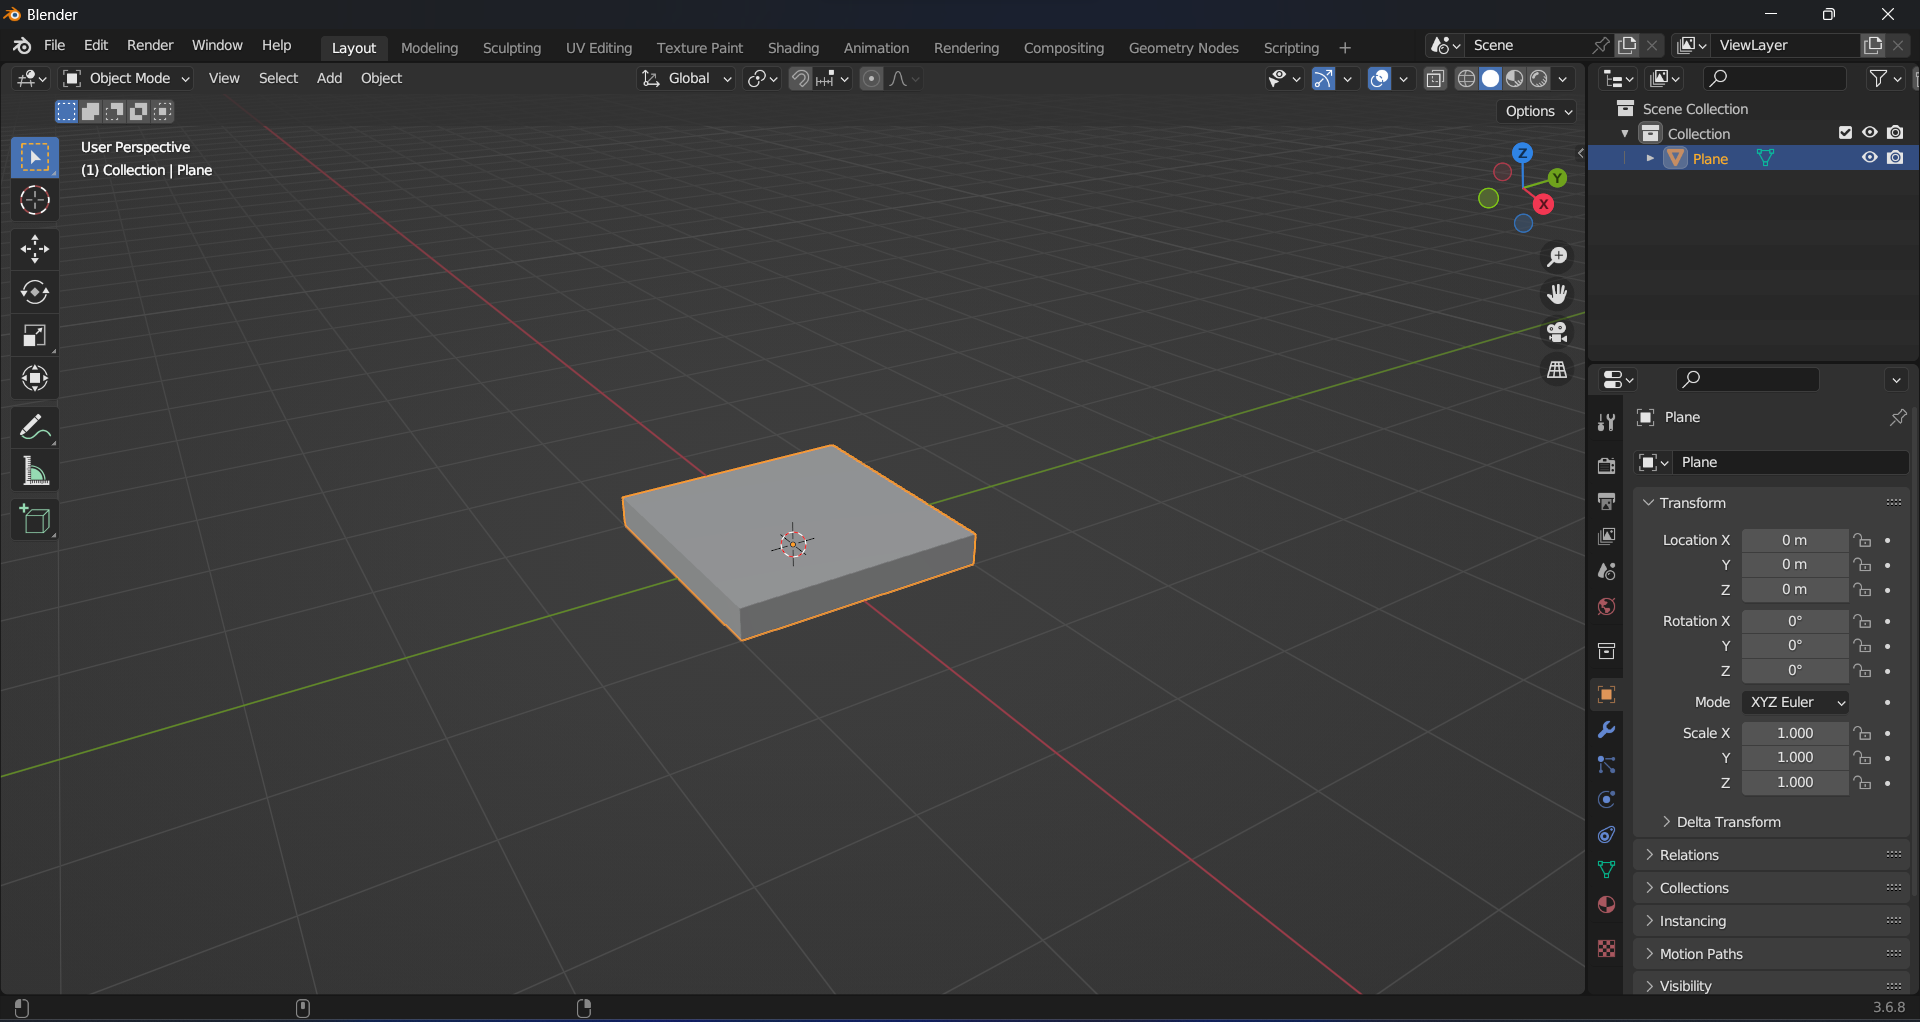
\includegraphics[width=1\textwidth]{images/AusgangslageTaschenrechner.png}
    \caption{Ausgangslage innerhalb von Blender}
    \label{fig:Ausgangslage}
\end{figure}

Durch diesen Prozess der Initiierung wurde die Grundlage für die folgenden Schritte der Modellierung gelegt, die in weiteren Abschnitten detaillierter beschrieben werden.

\subsubsection*{Erste Schritte nach der Erstellung}
Nach Auswahl eines geeigneten Referenzbildes für das Taschenrechnermodell wurde dieses mithilfe des Add-Ons \textit{Images as Planes} in Blender eingefügt. Das Bild dient als Leitfaden für die Modellierung und wurde unterhalb des bereits vorhandenen Objekts platziert. Um eventuelle Unregelmäßigkeiten im Design zu vermeiden, wurde der Mirror Modifier aufgrund der symmetrischen Form des Taschenrechners angewendet. Durch diese Maßnahme werden alle Modellierungsaktionen, die auf der linken Seite durchgeführt werden, automatisch auf die rechte Seite gespiegelt. Dadurch wird die Effizienz und Genauigkeit des Modellierungsprozesses erhöht.

\subsubsection*{Extrahieren als Modellierungswerkzeug}
Extrahieren \footnote{Blender \cite{Extrahieren}} ist ein Werkzeug im Edit-Modus von Blender. Es dient dazu, ausgewählte Punkte zu duplizieren und zu verschieben, während die ursprünglichen Punkte der Bearbeitungslinie erhalten bleiben.
Für die Verwendung des Extrahieren-Werkzeugs ist ein Verständnis der grundlegenden Konzepte des Edit-Modus in Blender sowie eine präzise Auswahl der zu extrahierenden Punkte erforderlich, um die gewünschten Modifikationen am Modell vorzunehmen. Während des Modellierungsprozesses ist es von entscheidender Bedeutung, unbeabsichtigte Extraktionen zu vermeiden, da diese dazu führen können, dass duplizierte Vertices über bereits vorhandenen liegen. Dies kann nicht nur die weitere Bearbeitung des Modells beeinträchtigen, sondern auch zu einer unnötigen Zunahme der Anzahl der Vertices führen.

\subsubsection*{Weiterführung beim Taschenrechnermodell}
Im Anschluss begann die Modellierung durch Extrudieren eines Eckpunkts der Fläche, um grob der Form des Referenzbildes zu folgen.

\begin{figure}[H]
    \centering
    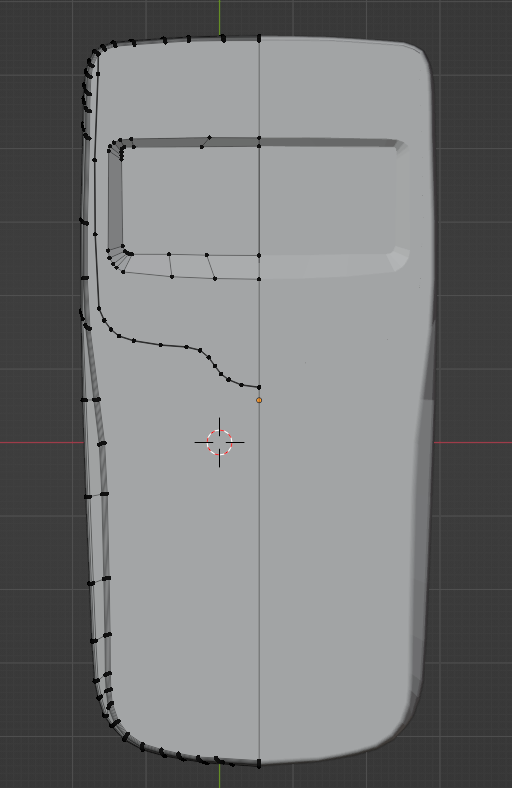
\includegraphics[width=0.4\textwidth]{images/basis.png}
    \caption{Taschenrechner mit Buttons in Blender}
    \label{fig:Basis}
\end{figure}

Nach Abschluss dieser groben Modellierungsschritte entstand das Grundgerüst des Taschenrechnermodells, wie in Abbildung \ref{fig:Basis} dargestellt. Die verschiedenen Eckpunkte (Vertices) werden im Edit-Modus von Blender als schwarze Punkte dargestellt. Durch den Mirror Modifier wird die Bearbeitung auf der linken Seite des Modells automatisch auf die rechte Seite gespiegelt, was eine symmetrische Form gewährleistet. Um dem Modell mehr Tiefe zu verleihen, wurde Extrudieren verwendet, um aus der ebenen Fläche eine dreidimensionale Struktur zu formen.

%quelle für literatur
%https://docs.blender.org/manual/de/dev/grease_pencil/modes/edit/point_menu.html#extrude

Als nächster Schritt steht die Modellierung der Knöpfe und anderer Funktionen des Taschenrechners an, um das Modell weiter zu verfeinern und seinem realen Gegenstück näherzukommen. Dazu wird der \textit{Array}-Modifier verwendet, da dieser es ermöglicht, ein Button-Modell zu entwerfen und dieses dann zu vervielfältigen. Dadurch wird die Modellierungszeit enorm reduziert und die gleichmäßige Platzierung der Buttons verbessert.

%quelle für literatur
%https://docs.blender.org/manual/en/latest/modeling/modifiers/generate/array.html
\subsubsection*{Einschub Array-Modifier}
Der Array-Modifier in Blender ermöglicht die Erstellung einer Reihe von Kopien eines Basisobjekts. Jede Kopie wird dabei auf eine vordefinierte Weise von der vorherigen Kopie versetzt. Der Modifier bietet eine Vielzahl von Optionen zur Anpassung der Positionierung und Ausrichtung der Kopien.
Die grundlegenden Funktionen des Array-Modifiers umfassen die Möglichkeit, Vertices in benachbarten Kopien zusammenzuführen, insbesondere wenn sie nahe beieinander liegen. Dadurch können nahtlose und konsistente Verbindungen zwischen den einzelnen Kopien hergestellt werden.
Eine wichtige Option des Array-Modifiers ist der sogenannte \textit{Fit Type}, der angibt, wie das Objekt dupliziert werden soll. Dies kann entlang einer Kurve, mit einer passenden Länge oder einer festgelegten Anzahl von Kopien erfolgen. Darüber hinaus kann eine relative oder feste Verschiebung entlang der x-, y- oder z-Achse definiert werden, um die Positionierung der Kopien weiter anzupassen.

\subsubsection*{Weiterführung beim Taschenrechnermodell}
\begin{figure}[H]
    \centering
    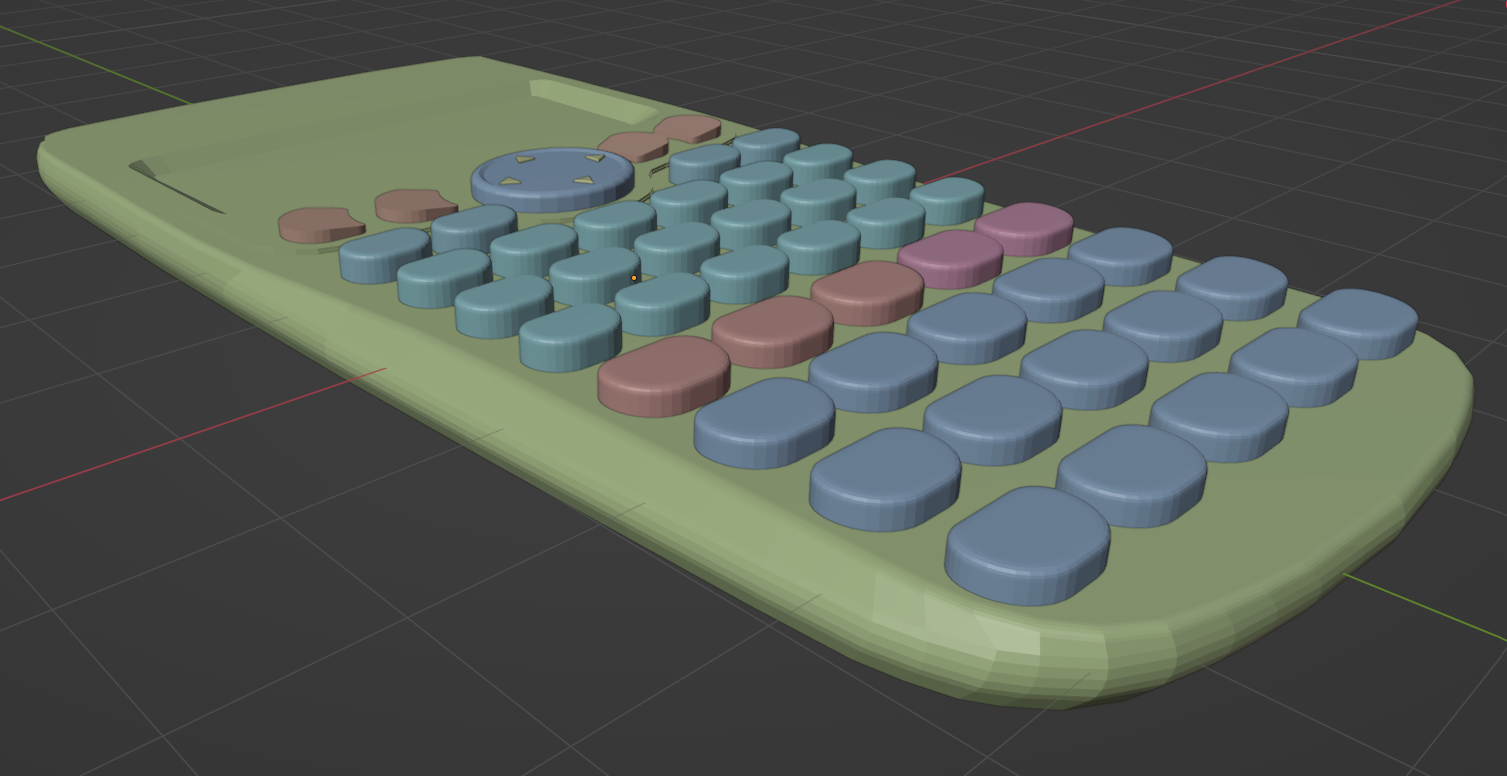
\includegraphics[width=0.8\textwidth]{images/taschenrechnermitbuttons.png}
    \caption{Taschenrechner mit Buttons in Blender}
    \label{fig:tcbuttons}
\end{figure}

Abbildung \ref{fig:tcbuttons} zeigt das Taschenrechnermodell in Blender mit den neu modellierten Buttons. Die dargestellten Farben dienen lediglich als visuelle Hilfestellung im Blender-Editor und stellen keine inhärenten Eigenschaften des Modells dar. Jedes neu erstellte Objekt wird automatisch mit einer zufälligen Farbe versehen, um eine einfachere Unterscheidung innerhalb der Szene zu ermöglichen.

Einige der Buttons im Modell wurden mithilfe des Array-Modifiers vervielfältigt. Dies gilt insbesondere für Buttons, die im Referenzbild die gleiche Größe, Funktion und Farbe aufweisen. Durch diese Technik ist es möglich, wiederkehrende Elemente effizient zu modellieren, indem eine einzelne Vorlage kopiert und entsprechend der gewünschten Anordnung angepasst wird.

Der aktuelle Stand des Modells lässt darauf schließen, dass die Modellierung größtenteils abgeschlossen ist. Der nächste Schritt besteht darin, dem Modell Farben oder Texturen hinzuzufügen, um ein realistischeres Aussehen zu erzielen. Dies kann durch Anwendung von Materialien und Texturen im Renderprozess erreicht werden, um dem Modell visuelle Tiefe und Detailtreue zu verleihen.

Die Fortführung des Modellierungsprozesses umfasst somit die Umsetzung der texturierten Oberfläche sowie mögliche Feinanpassungen, um das Modell weiter zu verbessern und an die Referenzvorlage anzupassen.

\subsubsection*{Hierarchie des fertiggestellten Modells}
In Blender wird die Hierarchie eines Modells als Baumstruktur dargestellt. Dabei ermöglichen verschiedene Unterteilungen und Kategorien eine übersichtliche Organisation. Die Struktur wird in Abbildung
\ref{fig:hierarchie} veranschaulicht. Das weiße Box-Symbol steht für eine Collection (Ordner).

\begin{figure}[H]
    \centering
    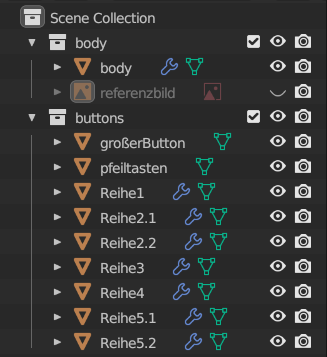
\includegraphics[width=0.5\textwidth]{images/hierarchietaschenrechner.png}
    \caption{Hierarchie des fertigen Taschenrechnermodells}
    \label{fig:hierarchie}
\end{figure}

\begin{itemize}
    \item Die \textbf{Scene Collection} ist die oberste Ebene, die das gesamte Modell enthält.
    \item Die \textbf{Body Collection} enthält das Hauptmodell des Taschenrechners, also die grundlegende Form.
    \item Die \textbf{Buttons Collection} umfasst alle Buttons, die auf dem Taschenrechner abgebildet sind.
    \item Die untergeordnete Struktur mit den orangefarbenen Dreiecken repräsentiert die eigentlichen Objekte innerhalb der jeweiligen Collections.
    \item Das \textbf{Referenzbild} ist ein importiertes Bild, das beispielsweise als Vorlage für das Modellieren verwendet wird.
\end{itemize}

In Abbildung \ref{fig:hierarchie} ist zu erkennen, dass ein Objekt ausgegraut ist. Dies bedeutet in dem Fall, dass das Objekt ausgeblendet wurde, da das Hauptmodell bereits fertiggestellt wurde und das Referenzbild nicht mehr benötigt wird. Das Referenzbild kann jedoch bei Bedarf aktiviert werden, beispielsweise zu Hilfe- oder Veranschaulichungszwecken.

Die hierarchische Darstellung der Elemente erleichtert die Organisation und Bearbeitung des Modells. Eine klare Strukturierung der verschiedenen Komponenten ermöglicht eine effiziente Arbeitsweise und hilft, den Überblick über die einzelnen Teile zu behalten.

\subsubsection*{Textur und Farbe des Taschenrechnermodells}
Für die Texturierung und Farbgebung des Modells diente das Referenzbild zur Orientierung. Das \textit{Eye-Dropper}-Werkzeug in Blender ermöglichte es, Farben gezielt aus dem Referenzbild auszuwählen und auf das entsprechende Modell anzuwenden. Durch Klicken auf einen bestimmten Bereich des Referenzbildes wurde die Farbe erfasst und dann auf den entsprechenden Bereich des Modells übertragen.

% https://docs.blender.org/manual/en/latest/interface/controls/buttons/eyedropper.html
Dieser Prozess wurde für jedes Element des Modells durchgeführt, um eine genaue Anpassung an die Farben und Texturen des Referenzbildes zu erreichen. Die Verwendung des Eye-Dropper-Werkzeugs ermöglichte eine präzise und konsistente Umsetzung der Farbgebung und trug dazu bei, dass das Modell möglichst authentisch und realitätsnah aussieht. Um noch bessere und realitätsnähere Textur zu gewährleisten, wurde ein Vorgang Namens \textit{UV-Mapping} durchgeführt.

%literatur https://docs.blender.org/manual/en/latest/modeling/meshes/editing/uv.html
%literatur https://all3dp.com/2/blender-uv-mapping-simply-explained/
%literatur https://de.wikibooks.org/wiki/Blender_Dokumentation:_UV-Mapping
\subsubsection*{UV-Mapping}
\textit{UV-Mapping} ist ein wichtiger Schritt im Texturierungsprozess von 3D-Modellen. Dabei werden Texturen auf dreidimensionale Objekte projiziert. Die Bezeichnungen \textit{U} und \textit{V} stehen dabei für die beiden Koordinatenachsen im zweidimensionalen Raum. In Blender gibt es dafür einen eigenen Editor mit einer spezifischen Benutzeroberfläche.

Während der Modellierung des Taschenrechnermodells wurde \textit{UV-Mapping} genutzt, um Texturen detailgetreu von einem Referenzbild auf die einzelnen Knöpfe und Tasten des Modells zu übertragen. Dieser Prozess ermöglicht es, die Beschriftungen und andere Details automatisch von der Textur abzuleiten, anstatt sie manuell für jedes Element erstellen zu müssen.

\begin{figure}[H]
    \centering
    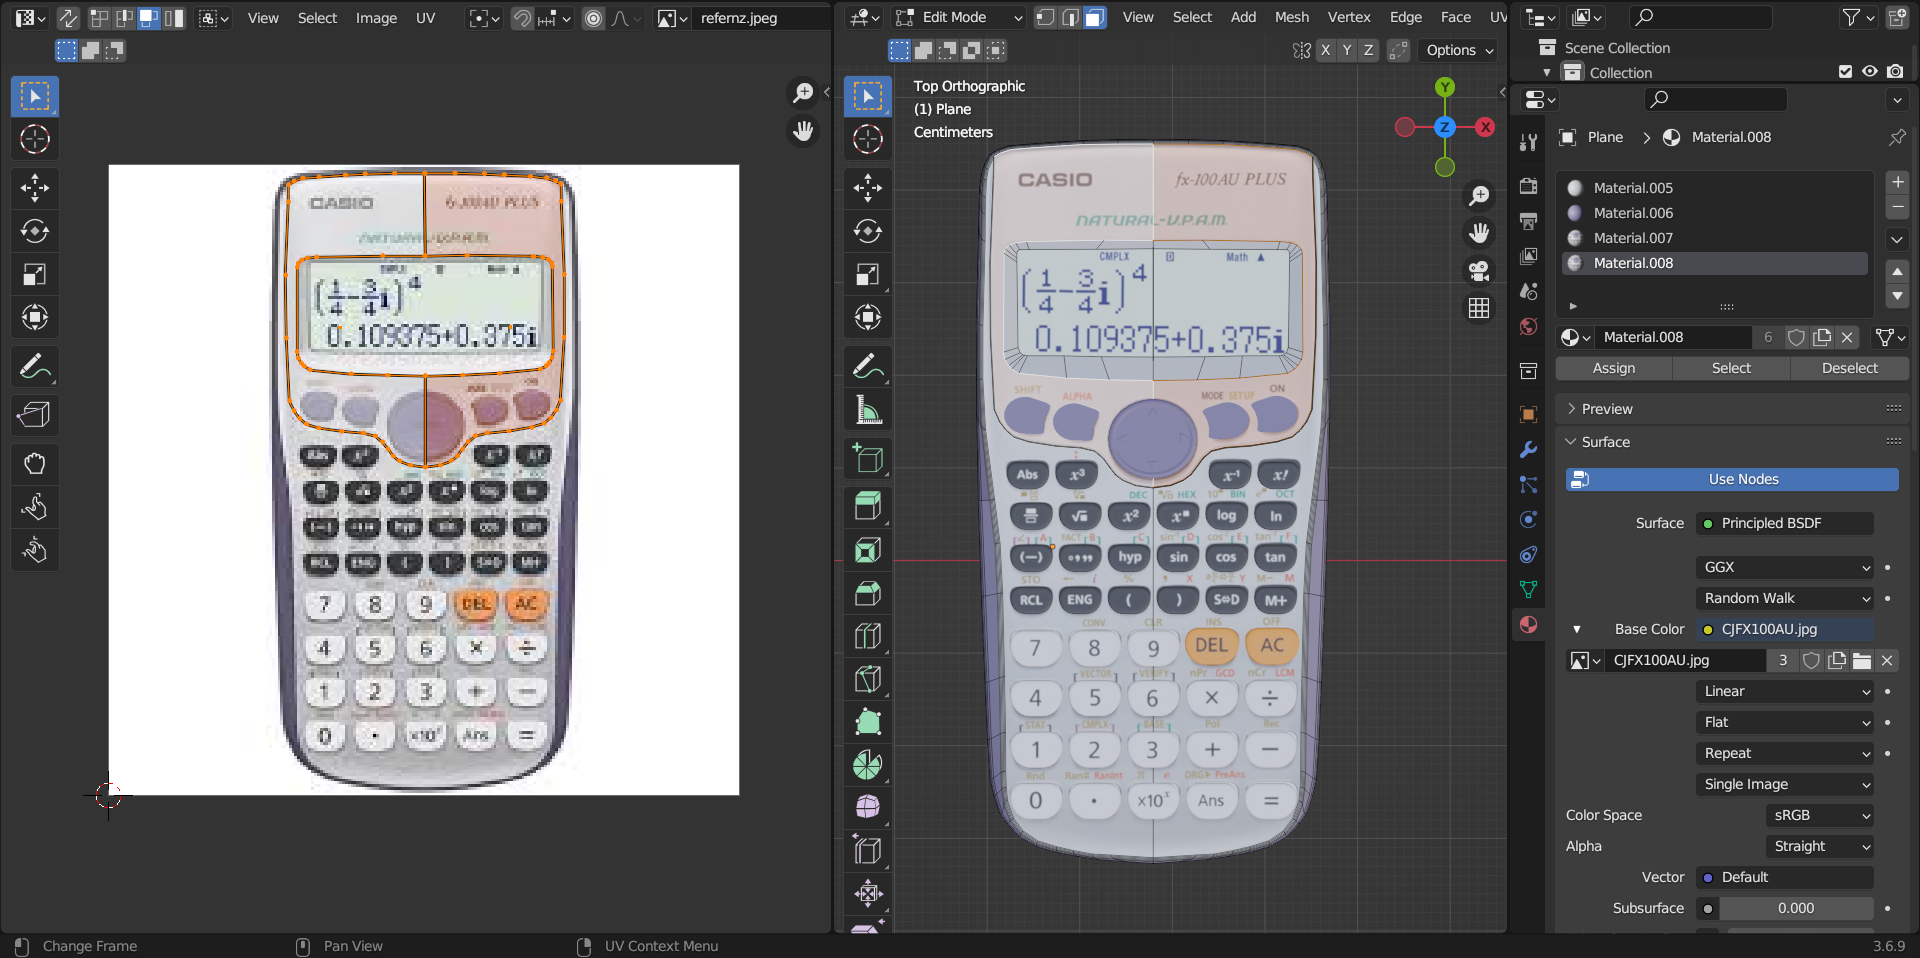
\includegraphics[width=1\textwidth]{images/uvmappingeditor.png}
    \caption{Ansicht des UV-Editing Editors in Blender}
    \label{fig:hierarchie}
\end{figure}

Die Abbildung zeigt den \textit{UV-Editing-Editor} in Blender. Mit diesem Editor können die UV-Maps der 3D-Modelle bearbeitet werden, indem die 3D-Geometrie auf eine zweidimensionale Ebene projiziert wird, um die Positionierung der Texturen zu steuern.

Als Beispiel wurde der obere Teil des Taschenrechners rund um den Bildschirm ausgewählt. Zunächst wird dem Bereich ein neues Material zugewiesen, das die Basisfarbe des Referenzbildes enthält. Anschließend wird das Referenzbild als Texturhintergrund im Editor ausgewählt, um es anzuzeigen.

Der nächste Schritt besteht darin, die ausgewählten Flächen des Modells aufzuteilen, denn die Erstauswahl in Blender legt die einzelnen Flächen übereinander. Dies geschieht durch Auswahl der Flächen im Editor und Anwendung der \textit{UV-Unwrap}-Funktion in Blender.

Nach dem \textit{UV-Unwrappen} werden die Flächen im Editor positioniert, um die Texturen und Beschriftungen korrekt auf das Modell zu projizieren, ohne dass sie abgeschnitten oder verzerrt wirken. Dieser Prozess ist zeitaufwendig, da er für jedes einzelne Element des Modells wiederholt werden muss. Dabei muss auch auf korrekte Skalierungen geachtet werden, um eine einheitliche Darstellung zu gewährleisten.

\textit{UV-Mapping} ist somit ein entscheidender Schritt bei der Erstellung realistischer 3D-Modelle, da es eine präzise Texturierung und Gestaltung ermöglicht.

\subsubsection{Restliche Modelle}
\begin{figure}[H]
    \centering
    \begin{minipage}[b]{0.20\textwidth}
        \centering
        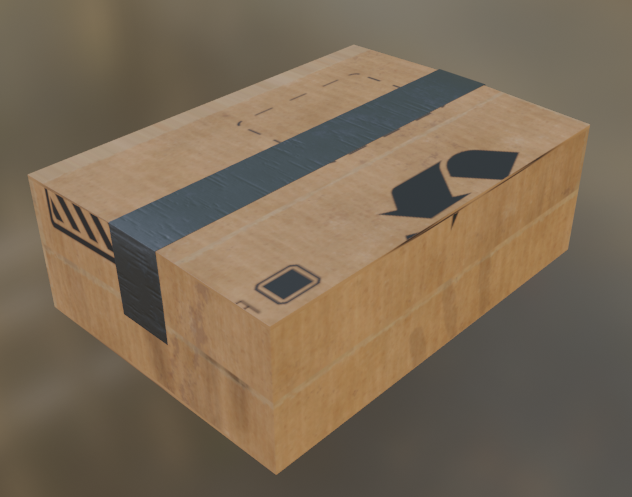
\includegraphics[width=3cm,height=3cm]{images/package.png}
    \end{minipage}
    \hfill
    \begin{minipage}[b]{0.20\textwidth}
        \centering
        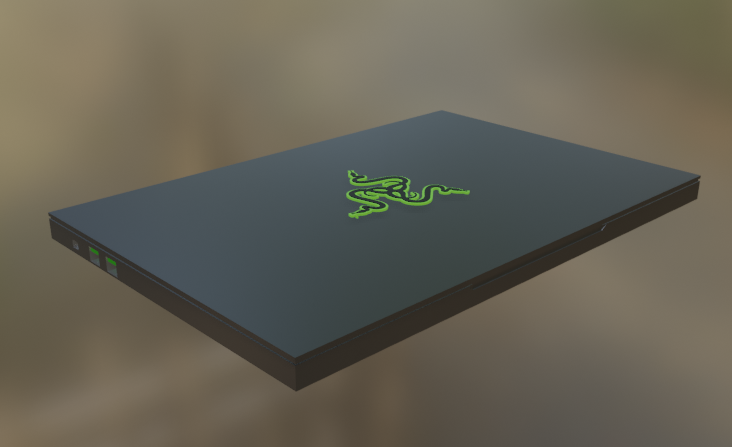
\includegraphics[width=3cm,height=3cm]{images/laptop.png}
    \end{minipage}
    \hfill
    \begin{minipage}[b]{0.20\textwidth}
        \centering
        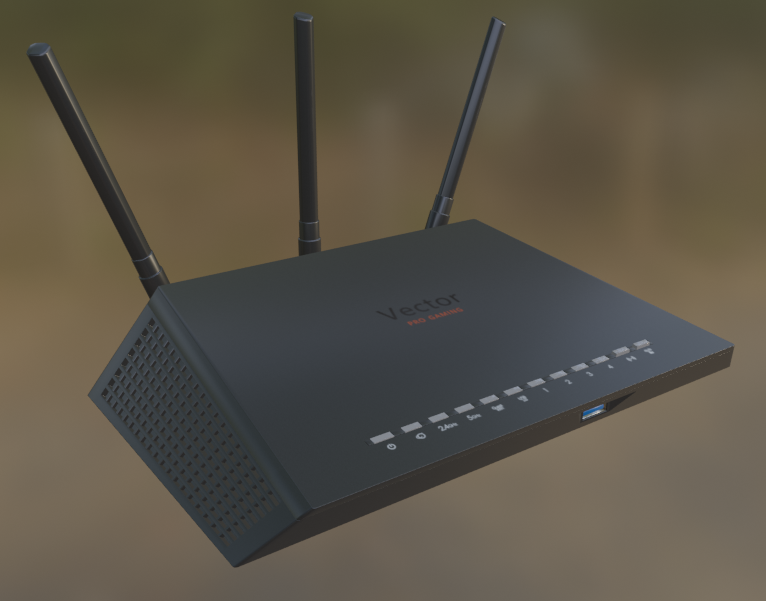
\includegraphics[width=3cm,height=3cm]{images/router.png}
    \end{minipage}
    \hfill
    \begin{minipage}[b]{0.20\textwidth}
        \centering
        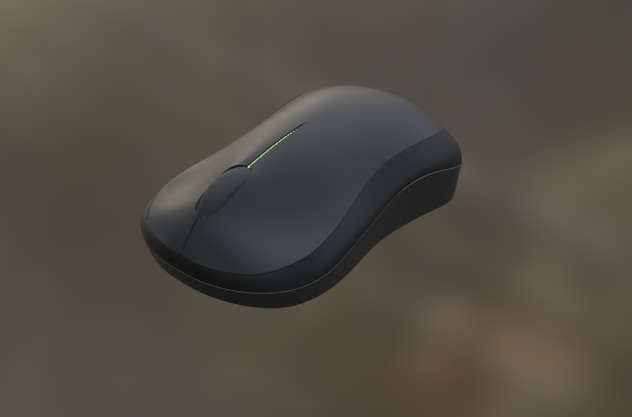
\includegraphics[width=3cm,height=3cm]{images/mouse.png}
    \end{minipage}
\end{figure}

\subsubsection*{Ping-Paket-Modell}
Das Ping-Paket-Modell wurde speziell für didaktische Zwecke auf das erste Anwendungsszenario konzipiert, um den Benutzern das grundlegende Konzept eines Daten-Pings zu veranschaulichen. Es dient dazu, die Übertragung von Daten zwischen zwei Endpunkten, beispielsweise Laptops, zu visualisieren. Das Modell besteht im Wesentlichen aus einem simplen Quader, ergänzt durch Details wie Paketklebeband, um eine realistische Darstellung zu erreichen. Bei der Texturierung wurde ein Amazon-Paket als Referenz verwendet.

\subsubsection*{Laptop-Modell}
Der Laptop stellt einen unverzichtbaren Gegenstand im zweiten Anwendungsszenario dar und ist ein essentielles Werkzeug für Schüler ab der 3. Klasse. Bei der Modellierung wurden zusätzliche Details wie USB-Ports und der Laptopständer berücksichtigt. Um den Aufwand zu minimieren, wurde der Laptop im geschlossenen Zustand modelliert, wodurch die Komplexität von Tastatur und Bildschirm vermieden wurde. Die Referenz für das Modell lieferte ein reales Laptop-Exemplar eines Projektmitglieds.

\subsubsection*{Router-Modell}
Die Modellierung des Routers war eine iterative Aufgabe, die mehrere Versionen erforderte, um ein realistisches und ansprechendes Modell zu erzielen. Das finale Modell repräsentiert einen Gaming-Router mit vielen Anschlüssen und Bedienelementen. Aufgrund der Vielzahl an Details war die Modellierung sehr anspruchsvoll und zeitaufwendig.

\subsubsection*{Maus-Modell}
Die Modellierung der Maus war eine Standardaufgabe, bei der der Mirror Modifier effektiv eingesetzt wurde, um die symmetrische Natur des Objekts zu betonen. Eine einfache Büromaus diente als Referenz für das Modell.


\begin{figure}[H]
    \centering
    \begin{minipage}[b]{0.20\textwidth}
        \centering
        
\includegraphics[width=3cm,height=3cm]{images/notizblock.png}
    \end{minipage}
    \hfill
    \begin{minipage}[b]{0.20\textwidth}
        \centering
        
\includegraphics[width=3cm,height=3cm]{images/stift.png}
    \end{minipage}
    \hfill
    \begin{minipage}[b]{0.20\textwidth}
        \centering
        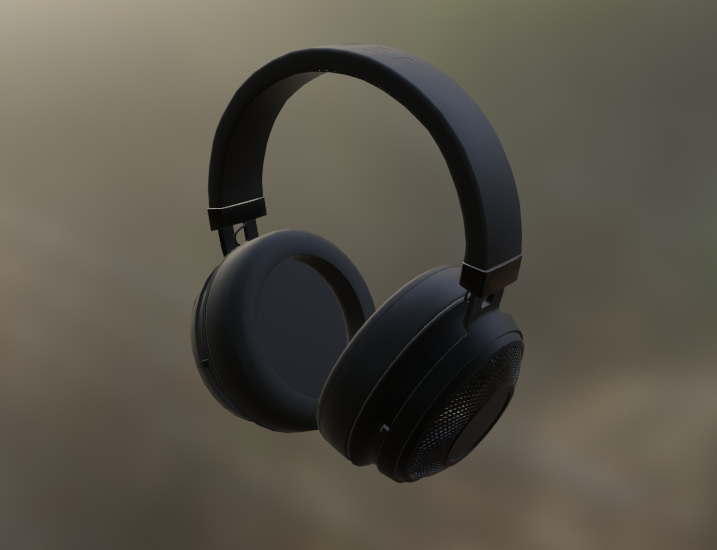
\includegraphics[width=3cm,height=3cm]{images/headphones.png}
    \end{minipage}
    \hfill
    \begin{minipage}[b]{0.20\textwidth}
        \centering
        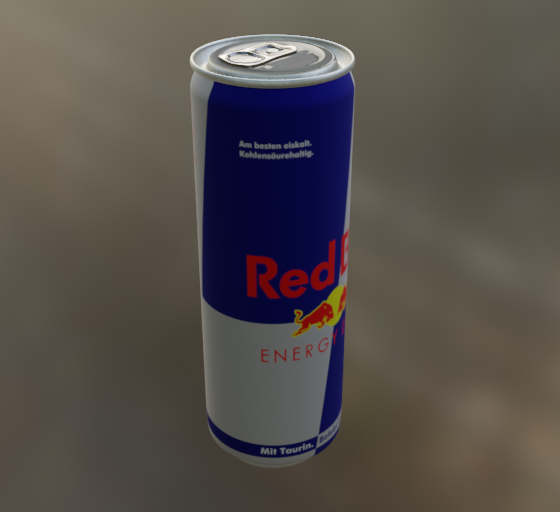
\includegraphics[width=3cm,height=3cm]{images/energy.png}
    \end{minipage}
\end{figure}

\subsubsection*{Notizblock-Modell}
Der Block ist ein wichtiger Gegenstand im schulischen Umfeld bis zur 3. Klasse, wenn noch keine Laptops verwendet werden. Während der Designphase ermöglichte der Array Modifier eine einfache Gestaltung der spiralförmigen Halterung der Blätter.

\subsubsection*{Stift-Modell}
Der Stift wurde einfach modelliert und erhielt eine unkomplizierte Texturierung mit einfachen Farben. Ein Buntstift diente als Referenz für das Modell.

\subsubsection*{Kopfhörer-Modell}
Die Modellierung der Kopfhörer erforderte aufgrund ihrer geschwungenen Form und der texturierten Oberfläche besondere Aufmerksamkeit. Das Modell durchlief zwei Phasen: zunächst eine Annäherung an das Referenzbild eines Gaming-Kopfhörers und dann eine Verfeinerung, einschließlich einer aufwendigen Lederstrukturtextur.

\subsubsection*{Dose-Modell}
Die Modellierung der Dose eines Energydrinks begann mit einem einfachen Zylinder, der dann anhand eines Referenzbildes geformt wurde. Besonderes Augenmerk wurde auf die Textur gelegt, wobei ein bekanntes Produktlabel als Referenz diente.

\newpage
\begin{figure}[H]
    \centering
    \begin{minipage}[b]{0.20\textwidth}
        \centering
        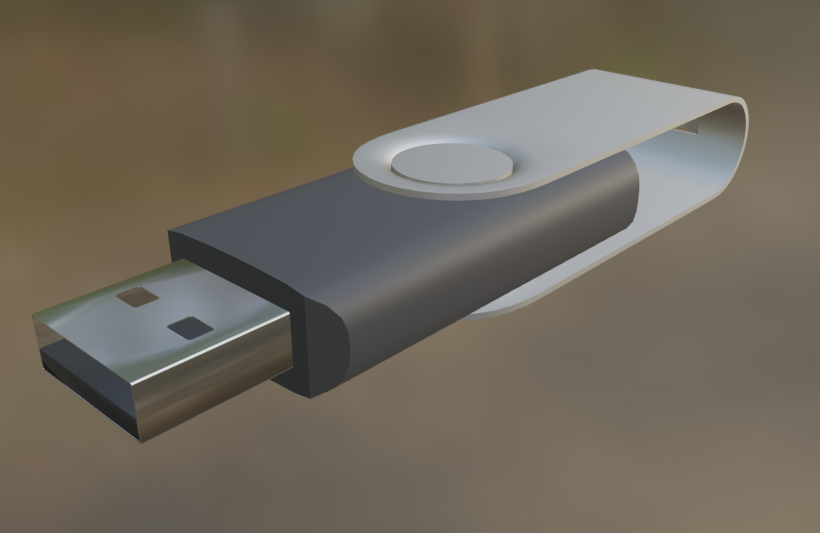
\includegraphics[width=3cm,height=3cm]{images/usb.png}
    \end{minipage}
    \hfill
    \begin{minipage}[b]{0.20\textwidth}
        \centering
        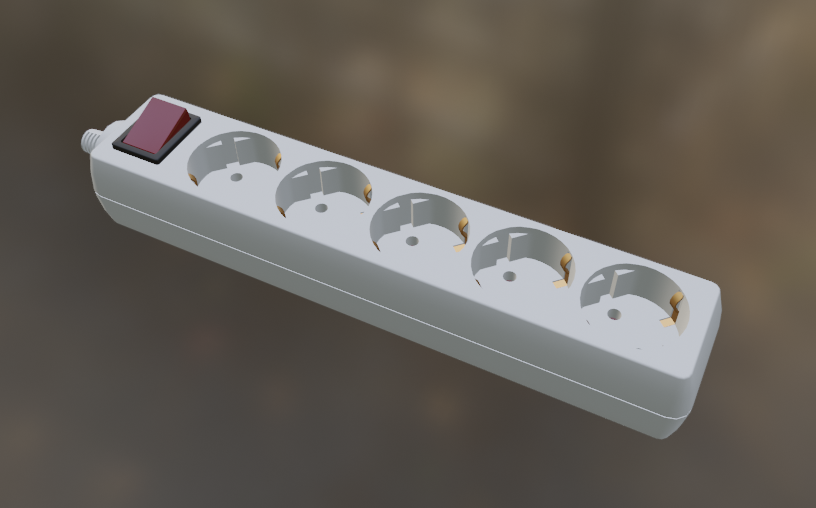
\includegraphics[width=3cm,height=3cm]{images/stromverteiler.png}
    \end{minipage}
    \hfill
    \begin{minipage}[b]{0.20\textwidth}
        \centering
        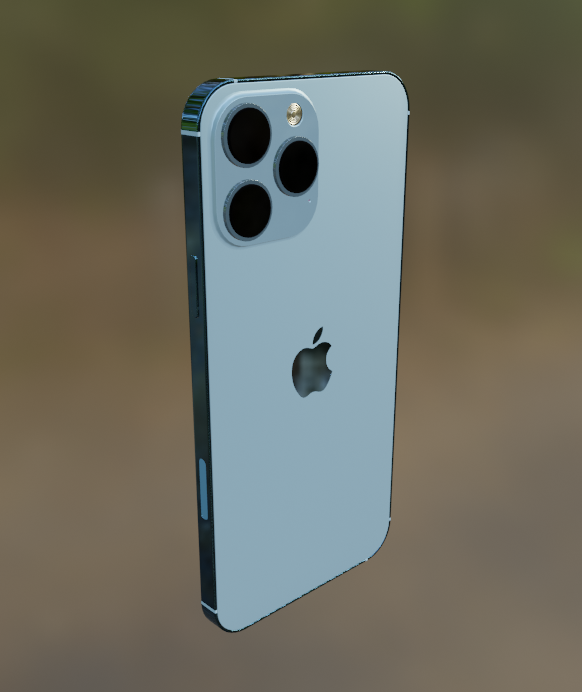
\includegraphics[width=3cm,height=3cm]{images/iphone.png}
    \end{minipage}
\end{figure}

\subsubsection*{USB-Stick-Modell}
Der USB-Stick wurde mit einer integrierten Halterung für zusätzliche Komplexität modelliert. Die Texturierung betonte einen metallischen Effekt, insbesondere für die Halterung und das vordere Teil des USB-Sticks.

\subsubsection*{Stromverteiler-Modell}
Der Stromverteiler wurde mit fünf Steckplätzen und einem Ein/Aus-Schalter modelliert, wobei der Fokus auf einfacher Funktionalität lag. Die Texturierung orientierte sich an einfachen weißen Steckerleisten.

\subsubsection*{Handy-Modell}
Das Handymodell orientierte sich an modernen iPhones von Apple und erforderte aufgrund seiner zahlreichen Details wie Kameras, Tasten und Mikrofoneinlässe eine sorgfältige Modellierung und Texturierung, um einen realistischen Eindruck zu erzeugen.


\section{Hauptmenü}
Im folgenden Abschnitt werden die Entwicklungsphasen beim Entwurf des Menüs erläutert. Es wird erklärt, welche Probleme dabei auftreten und worauf bei der Benutzeroberfläche (UI) und der Benutzererfahrung (UX) geachtet werden muss.
Es wird aufgeteilt in die Konzeption und Planung der Benutzeroberfläche bis hin zur finalen Umsetzung. Die iterative Entwicklung des Menüs durchlief mehrere Phasen, bei denen Entscheidungen zum Design des Layouts, des Farbschemas und der Interaktionselemente getroffen wurden.
Während der Entwicklung wurden regelmäßig Überprüfungen und Anpassungen durchgeführt, um sicherzustellen, dass das Menü den gestellten Anforderungen entspricht und eine optimale Benutzererfahrung bietet. Dabei wurden auch Rückmeldungen und Tests von Nutzern in die Iterationsschleife einbezogen, um mögliche Verbesserungspotenziale zu identifizieren und zu berücksichtigen.
Schließlich wurde das Menü in seiner endgültigen Version implementiert. Dabei wurde besonderes Augenmerk auf Funktionalität, Benutzerfreundlichkeit und Ästhetik gelegt. Durch diesen iterativen Entwicklungsprozess wurde sichergestellt, dass das Menü den Anforderungen entspricht und einen positiven Beitrag zur Gesamterfahrung des Spiels leistet.

\subsection{Erstentwurf}
Ursprünglich war geplant, das UI/UX-System mit einem sogenannten \textbf{Nahmenü} zu realisieren. Dieses folgt dem Nutzer in seiner Nähe und besteht in unserem Fall, aus drei primären Schaltflächen sowie einem Pin-Button. Das Nahmenü ist etwa auf Hüfthöhe des Benutzers positioniert und zeichnet sich durch eine vereinfachte Struktur aus, die eine intuitive Bedienung gewährleistet. Die Gestaltung des Menüs hat zum Ziel, Verwirrung zu vermeiden und dem Nutzer ohne umfassende Vorabinformationen klar zu machen, wie er die Anwendung verwenden kann.

\subsubsection*{Nahmenü}
Innerhalb von Unity bezeichnet der Begriff \textit{Nahmenü} eine vordefinierte Konstruktion, die mit bestimmten Skripten ausgestattet ist, um sicherzustellen, dass das Menü dem Benutzer in alle Richtungen folgt. Es werden von Unity bereitgestellte Skripte verwendet, die es ermöglichen, das Menü dynamisch an die Position des Nutzers anzupassen.\\
\\
Im Erstentwurf wurde das gesamte Menü ausschließlich innerhalb der Unity-Umgebung konstruiert. Dabei wurden sämtliche vorhandenen Schaltflächen und Funktionen aus den nativen Ressourcen von Unity zusammengesetzt. Dieser Ansatz führte zu einer konsistenten visuellen Gestaltung des Menüs. Allerdings waren die Möglichkeiten zur kreativen Gestaltung und Anpassung im Rahmen unseres individuellen Projekts stark begrenzt. Durch die ausschließliche Verwendung der internen Ressourcen von Unity wurden gewisse Einschränkungen hinsichtlich der Flexibilität und Individualisierungsmöglichkeiten des Menüs in Kauf genommen.

Obwohl diese Herangehensweise zu einem homogenen Erscheinungsbild des Menüs führte, war es wichtig, eine Balance zwischen visueller Einheitlichkeit und der Notwendigkeit individueller Anpassungsmöglichkeiten zu finden. Diese Herausforderung verdeutlicht die Bedeutung einer flexiblen und erweiterbaren Architektur für die Benutzeroberfläche, um den Anforderungen und Zielen des Projekts gerecht zu werden.
\begin{figure}[H]
    \centering
    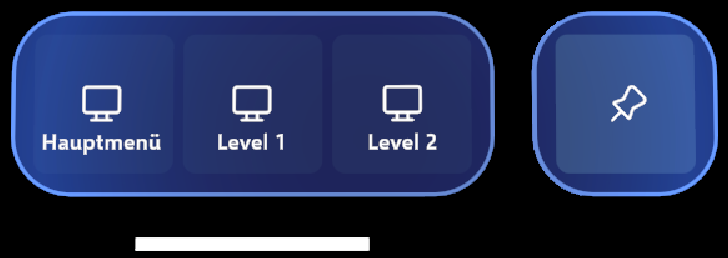
\includegraphics[width=0.8\textwidth]{images/menubarversion1.png}
    \caption{Darstellung des Erstentwurfes im Unity Editor}
    \label{fig:menübar}
\end{figure}

Die Abbildung \ref{fig:menübar} zeigt den ersten Entwurf des Menüs, das eine wichtige Schnittstelle für den Nutzer darstellt, um zwischen verschiedenen Szenarien zu navigieren. Die Struktur des Menüs bleibt unabhängig vom jeweiligen Spiellevel konstant, was zur Simplifizierung und Klarheit beiträgt. Die primären Schaltflächen auf der linken Seite dienen der Initiierung des Ladevorgangs für die verschiedenen Spielszenarien. Hervorzuheben ist der Pin-Button in Kombination mit dem darunterliegenden weißen Balken. Diese beiden Funktionen gemeinsam ermöglichen es dem Benutzer, das Menü an gewünschten Positionen zu verankern und bietet somit Flexibilität bei der Positionierung entsprechend individueller Präferenzen. Ein solcher Einsatz ist von Vorteil, wenn externe Objekte die Nutzbarkeit des Menüs beeinträchtigen könnten, wie zum Beispiel im Szenario des Platznehmens an einem Tisch, wo das Menü ungünstigerweise mit dem Tisch kollidieren könnte und somit die Nutzererfahrung beeinträchtigt werden würde.

\subsubsection{Probleme beim Erstentwurf}
\subsubsection*{Problem 1 - Fehlende Dokumentation}
Das Hauptziel bei dem Konzept des ersten Menüs, bestand darin, ein benutzerfreundliches Menü zu gestalten, das alle erforderlichen Funktionen enthält und dennoch übersichtlich ist. Nach mehreren Iterationen und Tests mit Testpersonen, die nicht mit dem Projekt vertraut waren, stellte sich heraus, dass der ursprüngliche Entwurf erhebliche Mängel bei der Dokumentation und Erklärung der verschiedenen Anwendungsszenarien und ihrer jeweiligen Aufgaben aufweist. Es wurde bemängelt, dass Benutzer lediglich zwischen den einzelnen Leveln wechseln können, ohne klare Informationen darüber zu erhalten, worum es in den einzelnen Leveln geht und welche Aufgaben diese beinhalten.

Diese Feststellung verdeutlicht eine wesentliche Lücke in der Benutzerführung und information innerhalb des Menüsystems. Die unzureichende Dokumentation der Level und ihrer Ziele führt zu einer fehlenden Orientierung für die Benutzer und kann sich negativ auf ihre Erfahrung auswirken. Das Menü sollte nicht nur als Navigationswerkzeug dienen, sondern auch als Informationsquelle, die dem Benutzer eine klare Vorstellung über den Spielverlauf und die zu erreichenden Ziele vermittelt.

Die Identifizierung dieses Problems betont die Wichtigkeit einer umfassenden Benutzerbeobachtung und -evaluation während des Designprozesses. Dadurch wird sichergestellt, dass das entwickelte Benutzeroberflächensystem den Bedürfnissen und Erwartungen der Zielgruppe entspricht. Eine zielgerichtete Überarbeitung des Menüs ist erforderlich, um die fehlende Dokumentation der Anwendungsszenarien und ihrer Aufgaben zu adressieren und somit die Benutzererfahrung zu verbessern.

Bei Testdurchführungen ohne Entwickler aus dem Projektteam kam es wiederholt zu Unklarheiten bei den Benutzern, insbesondere während des ersten Durchlaufs, bezüglich der zugewiesenen Aufgaben. Während der Nutzung der HoloLens-Anwendung gab es vermehrt Anfragen seitens der Benutzer an das Projektteam aufgrund von Unklarheiten. Dies lässt vermuten, dass die Anwesenheit von Entwicklern im Projektteam einen signifikanten Einfluss auf die Benutzererfahrung und Effektivität der HoloLens-Anwendung hat.


\subsubsection*{Problem 2 - Falsche Wahl des Menütyps}
Während des Testprozesses stellte sich heraus, dass das Navigationsmenü oft eine Behinderung darstellte, insbesondere für Entwickler, die Funktionen wiederholt testeten und Anwendungsszenarien neu luden. Das ständige Verschieben des Menüs zur Seite erwies sich als zeitraubend und störte den Arbeitsfluss erheblich. Die ursprüngliche Intention, das Navigationsmenü zur Erleichterung der Interaktion zwischen Benutzer und Spielumgebung einzuführen, erwies sich somit als kontraproduktiv.

Es ist wichtig, die Auswirkungen von Benutzeroberflächenelementen auf den Entwicklungsprozess zu berücksichtigen, um ein reibungsloses Testen und Experimentieren zu gewährleisten. Eine effiziente und produktive Arbeitsweise des Entwicklerteams hängt davon ab. Die Notwendigkeit einer kontinuierlichen Evaluation und Optimierung von UI/UX-Komponenten während des gesamten Entwicklungszyklus wird durch dieses Problem verdeutlicht.

Dieses Problem verdeutlicht, dass der Erstentwurf und die ursprüngliche Konzeption hauptsächlich auf die Innovation und Neuheit des Menüdesigns abzielten, anstatt den Fokus auf die funktionale Nützlichkeit zu legen. Der einfache und kompakte Menütyp erwies sich als unzureichend, um eine umfassende und übersichtliche Dokumentation der Anwendungsszenarien zu integrieren. Folglich war eine Migration zu einem alternativen Menüansatz erforderlich. Diese Beobachtung verdeutlicht die Bedeutung einer ausgewogenen Gestaltung von Benutzeroberflächen in Mixed-Reality-Systemen. Es ist wichtig, dass nicht nur ästhetische Innovationen verfolgt werden, sondern auch die tatsächliche Benutzererfahrung und -effizienz in Betracht gezogen wird. Die Reflexion über diesen Prozess bietet Einsichten in die iterative Entwicklung von Benutzerschnittstellen und die Anpassung an die Anforderungen und Rückmeldungen der Benutzer.

\subsection{Finalversion des Menüs}
Die endgültige Version des Menüs wurde entwickelt, um die Mängel des ursprünglichen Entwurfs anzugehen und idealerweise vollständig zu beheben. Dieses neue Konzept wurde durch eine umfassende Analyse populärer AR/VR-Spiele wie zum Beispiel \textit{Beat Saber} geleitet, um die Gründe für die verbesserte Benutzererfahrung in diesen Kontexten zu untersuchen. Dabei wurden spezifische Merkmale und Designentscheidungen identifiziert, die einen signifikanten Einfluss auf die Zufriedenheit der Anwender haben.

Basierend auf vorangegangenen Recherchen wurde entschieden, das neue Menü in zwei klar definierte Bereiche zu unterteilen. Dies gewährleistet eine deutliche Unterscheidung des Hauptmenüs sowie eine klare Orientierung bezüglich der Navigation. Insbesondere innerhalb der Anwendungsszenarien wurde ein minimalistisches und unaufdringliches Menü implementiert, um den Fokus der Benutzer uneingeschränkt auf die auszuführenden Tätigkeiten zu lenken. Diese Designstrategie hat zum Ziel, die kognitive Belastung der Benutzer zu reduzieren und eine nahtlose Integration der Menüfunktionalitäten in den jeweiligen Nutzungskontext zu ermöglichen.

Das Ergebnis ist ein ansprechendes und benutzerorientiertes Menükonzept, das die Gesamterfahrung des Spiels verbessert und den Erwartungen der Zielgruppe gerecht wird.

\subsubsection{Finalversion Menü - Hauptmenü}
Auf dieser Grundlage wurde das Design des Menüsystems vollständig überarbeitet, wobei der erste Schritt bereits die vollständige Entfernung der Idee des Nahmenüs beinhaltete.

Anstelle des Nahmenüs wurden vorgefertigte Objekte in das Hauptmenü integriert, welche zuvor mit Blender modelliert wurden. Die Entscheidung, vorgefertigte Objekte aus Blender zu importieren, bietet eine breite Palette an Gestaltungsmöglichkeiten und ermöglicht es, das Menü visuell ansprechend und einladend zu gestalten. Außerdem trägt die Integration dieser Objekte dazu bei, das Menü intuitiver und zugänglicher zu machen, da sie dem Benutzer klare Anhaltspunkte und Handlungsmöglichkeiten bieten.

\begin{figure}[H]
    \centering
    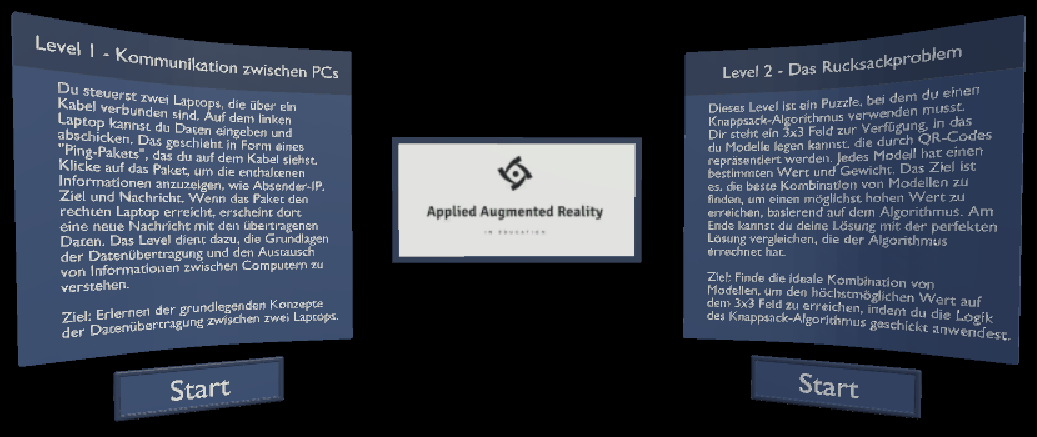
\includegraphics[width=1\textwidth]{images/menuversion2.png}
    \caption{Darstellung des finalen Menüs im Unity Editor}
    \label{fig:menuversion2}
\end{figure}

Die in der Abbildung \ref{fig:menuversion2} dargestellten Objekte bestehen aus zwei separaten Tafeln, die durch unser Diplomarbeitslogo voneinander getrennt sind. Jede Tafel enthält den Titel des Anwendungsszenarios sowie einen vorgefertigten Startbutton.  In Unity wurde ein unsichtbarer, aber dennoch klickbarer Button mit exakt denselben Dimensionen wie das Modell des Startbuttons an der entsprechenden Stelle platziert. Das Skript \textit{SceneChange.cs}, welches für die Szenenwechsel-Funktionalität verantwortlich ist, ist diesem Button angehängt.

\begin{figure}[H]
    \centering
    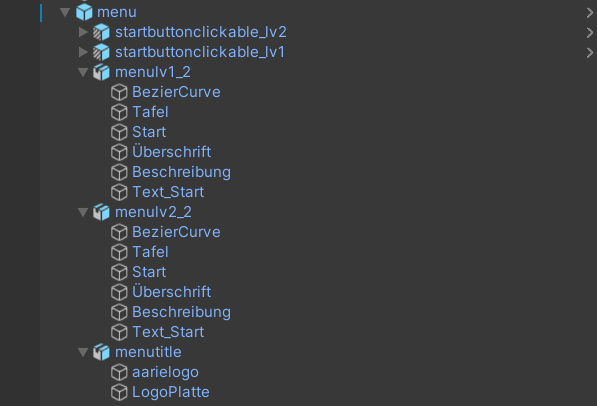
\includegraphics[width=0.8\textwidth]{images/hierarchiemenuunity.png}
    \caption{Darstellung der Hierarchie des finalen Menüs im Unity Editor}
    \label{fig:hierarchiemenuunity}
\end{figure}

In der Abbildung \ref{fig:hierarchiemenuunity} ist die Hierarchie des Hauptmenüs im Unity Editor zu sehen. Dem Prefab \textbf{menu} sind dabei 5 einzelne Objekte zugewiesen. Die Prefabs \textbf{startbuttonclickable\_lv1/2} sind die in Unity erstellten unsichtbaren Buttons, die dafür zuständig sind den vormodellierten Buttons eine Funktion zu geben. Darunter zu sehen sind die 3 verschiedenen Assets, welche aus Blender importiert wurden. Diese bestehen jeweils aus den verschiedenen Einzelteilen, welche in Unity als Gameobjects dargestellt werden. Die \textbf{BezierCurve} ist eine spezielle Art von Kurve welche in Blender für die leichte Wölbung der Tafeln genutzt wurde.

\subsubsection{Finalversion Menü - Anwendungsszenario}
Im Gegensatz zum Erstentwurf, der ein einheitliches Menü für alle Anwendungsszenarien vorsah, weist diese Version eine Differenzierung auf. Die Entscheidung, das Menü innerhalb der einzelnen Szenarien anzupassen, wurde getroffen, um die volle Aufmerksamkeit des Benutzers auf das jeweilige Level und die darin ausgeführten Aktivitäten zu lenken. Aus diesem Grund wurde ebenfalls das Nahmenü aus den Szenarien entfernt und durch ein simples Handmenü ersetzt.

\begin{figure}[H]
    \centering
    
\includegraphics[width=0.8\textwidth]{images/backbutton.png}
    \caption{Darstellung des finalen Menüs im Anwendungsszenario im Unity Editor}
    \label{fig:backbutton}
\end{figure}

Wie in der Abbildung \ref{fig:backbutton} gezeigt, besteht dieses Menü ausschließlich aus einem Zurück-Button, der den Benutzer zum Hauptmenü zurückführt. Das Handmenü wurde so konzipiert, dass es nur dann sichtbar ist, wenn der Benutzer es benötigt oder aktivieren möchte.  Der Zurückbutton wird erst sichtbar, wenn der Benutzer seine linke Hand umdreht und auf die Handfläche schaut.

Diese Funktionalität hat zum Ziel, die Benutzerinteraktion intuitiver und kontextbezogener zu gestalten. Hierfür wird Bewegungserkennung und Blickrichtungserkennung genutzt, um das Handmenü nur dann einzublenden, wenn der Benutzer aktiv nach einem Navigationsmittel sucht. Dadurch wird die visuelle Ablenkung minimiert und die Benutzererfahrung optimiert, indem nur relevante Informationen und Interaktionselemente präsentiert werden, wenn sie benötigt werden.

\subsubsection{Setzen des Menüs}
Beim Erstentwurf gab es keine Probleme beim Wechseln zwischen den Szenen beziehungsweise dem Laden in das Hauptmenü, jedoch muss man in der neuen Version darauf achten das Menü richtig zu setzen. Dafür muss man die Modelle im richtigen Moment und an der richtigen Stelle in der richtige Szene selbstständig instanzieren, deshalb wurde extra für diesen Fall das \textit{MenuSpawn.cs} Skript geschrieben.

\begin{lstlisting}[style=csharp, caption=Menueinstanzierung bei Neuladen., label=code:spawnmenu]
using System.Collections;
using System.Collections.Generic;
using UnityEngine;

public class SpawnPrefab : MonoBehaviour
{
    public GameObject menu;

    void Start()
    {
        SpawnPrefabMenu();
    }

    void SpawnPrefabMenu()
    {
        Vector3 cameraPosition = Camera.main.transform.position;
        Vector3 spawnPosition = new Vector3(cameraPosition.x, cameraPosition.y, cameraPosition.z + 1f);
        Instantiate(menu, spawnPosition, Quaternion.identity);
        menu.SetActive(true);
    }
}
\end{lstlisting}

Beim Start der Anwendung wird die Methode \textit{SpawnPrefabMenu()} ausgeführt. Diese Methode ist für die Positionierung des Menüs verantwortlich. Die im Codeabschnitt \ref{code:spawnmenu} ersichtlichen Positionsvektoren sind einerseits dafür zuständig, die aktuelle Kameraposition zu ermitteln, aber auch eine neue Spawnposition zu setzen, die um 1 auf der z-Achse versetzt ist, so dass das Menü vor dem Benutzer erscheint. Der Funktionsaufruf \textit{Instantiate} ist dafür verantwortlich, dass das Menü an der jeweiligen Spawnposition gesetzt wird. Anschließend wird das zuvor versteckte Menü mit \textit{menu.SetActive(true)} aktiviert, so dass der Benutzer es sehen und mit ihm interagieren kann.

%\subsection{Vergleich der Menüentwürfe} (vielleicht mach ich das noch)
\subsection{Laden der Level}
Um den Buttons eine Funktion zuzuweisen, wird ein Skript benötigt, das aktiviert wird, sobald ein Button gedrückt wird.
Im vorliegenden Fall ist das Skript \textit{SceneChange.cs} für den Wechsel zwischen den verschiedenen Anwendungsszenarien verantwortlich.
Wenn einer der Buttons im Hauptmenü gedrückt wird, wird dieses Skript ausgeführt. Die Spielszene wird im \textit{Unity Inspector}
festgelegt. Der Code greift auf die Variable zu, die den Namen der Szene enthält, wie sie zuvor im Inspector benannt wurde.

\begin{figure}[H]
    \centering
    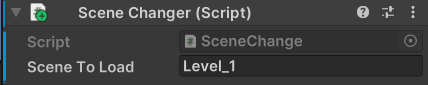
\includegraphics[width=0.6\textwidth]{images/sceneToLoad.png}
    \caption{Darstellung der SceneToLoad Variable, anhand des Level1 Buttons.}
    \label{fig:scenetoload}
\end{figure}

Für den linken Button im Hauptmenü ist beispielsweise die Spielszene \textit{Level1} vorgesehen, während für den rechten
Button die Szene \textit{Level2} zugewiesen ist. Durch diese Konfiguration im Inspector wird die Flexibilität gewährleistet,
Szenen dynamisch anzupassen, ohne dass Änderungen am eigentlichen Skript vorgenommen werden müssen. Dies ermöglicht eine
effiziente Verwaltung und Anpassung der Spielinhalte während des Entwicklungsprozesses.

\begin{lstlisting}[style=csharp, caption=Auf Knopfdruck Szene wechseln., label=code:scenechange]
using UnityEngine;
using UnityEngine.SceneManagement;

public class SceneChanger : MonoBehaviour
{
    public string sceneToLoad;

    public void ChangeScene()
    {
        if(SceneManager.GetActiveScene().name != sceneToLoad)
        {
            PlayerPrefs.DeleteAll();
            SceneManager.LoadScene(sceneToLoad, LoadSceneMode.Single);
        }
    }
}
\end{lstlisting}

Das vorliegende Skript hat eine vergleichsweise einfache Struktur. Die Variable \texttt{public string sceneToLoad} dient als Empfänger für den Namen der zu ladenden Szene, welcher im Unity-Inspector individuell für jede Szene festgelegt werden kann. Um den Szenenwechsel zu initiieren, wird die Methode \texttt{ChangeScene()} aufgerufen. Zunächst wird in dieser Methode geprüft, ob die aktive Szene, die durch \texttt{SceneManager.GetActiveScene()} ermittelt wird, mit der zu ladenden Szene übereinstimmt. Falls dies nicht der Fall ist, werden alle gespeicherten PlayerPrefabs mittels \texttt{PlayerPrefs.DeleteAll()} gelöscht. Dieser Schritt ist von entscheidender Bedeutung, um potenzielle Komplikationen im Zusammenhang mit dem HoloLens-Cache während des Szenenwechsels zu vermeiden.

Nachdem die Prefabs bereinigt wurden, wird die definierte Szene mit der Methode \texttt{SceneManag er.LoadScene()} geladen. Dabei wird die Ladeoption \texttt{LoadSceneMode.Single} verwendet, um sicherzustellen, dass nur die angegebene Szene aktiv geladen wird und keine anderen Szenen im Hintergrund verbleiben. Diese präzise Steuerung des Ladevorgangs zielt darauf ab, die Performance und Stabilität der Anwendung auf der HoloLens-Plattform zu optimieren und potenzielle Konflikte zwischen Szeneninhalten zu vermeiden.

\subsection{UI/UX}
Die Gestaltung der Benutzeroberfläche und die damit verbundene Benutzererfahrung sind wesentliche Aspekte bei der Konzeption und Entwicklung von Software. Eine bewährte Strategie besteht darin, sich an populären und gleichgerichteten Anwendungen zu orientieren, insbesondere im Bereich der Augmented- oder Virtual Reality. Es wird darauf geachtet, komplexe und verwirrende Menüstrukturen zu vermeiden und eine konsistente Farbpalette über die gesamte Benutzeroberfläche hinweg zu verwenden.

Diese Herangehensweise basiert auf der Erkenntnis, dass erfolgreiche Anwendungen in ähnlichen Domänen oft bewährte Designprinzipien und Interaktionsmuster aufweisen, die sich positiv auf die Benutzerakzeptanz und -zufriedenheit auswirken können. Durch die Anpassung an gängige Standards und Trends in der Branche kann das Risiko von Benutzerirritationen und -ablehnungen minimiert werden. Gleichzeitig wird eine vertraute und angenehme Benutzererfahrung gefördert.

Es ist wichtig zu betonen, dass eine solche Inspiration von bestehenden Anwendungen nicht als direkte Kopie verstanden werden sollte, sondern vielmehr als Quelle für Anregungen und bewährte Praktiken, die in einem eigenständigen und angepassten Kontext implementiert werden können. Auf diese Weise kann die Effektivität und Attraktivität der Benutzeroberfläche optimiert werden, um die Bedürfnisse und Erwartungen der Zielgruppe bestmöglich zu erfüllen.



\section{Nachrichtenaustausch Anwendungsscenario} \marginpar{\small(\rightarrow) Schoditsch}
In diesem Szenario wird das IT-Grundprinzip des Nachrichtenaustausches illustriert. Zwei PCs sind in einer realen Umgebung durch ein rotes Kabel miteinander verbunden, wobei auf jedem PC dieselbe Website geöffnet ist. Der Benutzer trägt eine HoloLens 2 und erhält die Aufforderung, das rote Kabel zu betrachten. Nach einem Countdown wird ein Foto der Umgebung aufgenommen und anschließend verarbeitet. Dabei werden Raycasts eingesetzt, um die exakte Position des roten Kabels in der physischen Welt zu bestimmen. Sobald die Position des Kabels erkannt wurde, kann der Benutzer über die Website auf den beiden PCs eine Nachricht senden. Diese Nachricht wird dann in Form eines Pakets für den Hololens 2 Benutzer visualisiert
Der Benutzer hat außerdem die Möglichkeit, auf das Paket zu drücken, um die Informationen wie Absender und Nachricht einzusehen.

\subsection{Aufbau von Nachrichtenaustausch Anwendungsscenario}
In diesem Abschnitt wird detailliert beschrieben, wie die Unity-Szene aufgebaut ist, welche Rollen und Funktionen die einzelnen GameObjects haben und wie sie miteinander interagieren, um die gewünschte Funktionalität der Szene zu erreichen.

\begin{figure}[H]
    \centering
    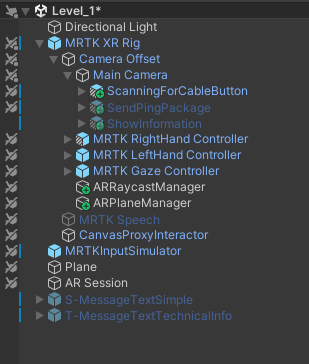
\includegraphics[scale=1]{images/Level1Hierarchy.png}
    \caption{Hierarchie des Nachrichtenaustausch Levels im Unity Editor.}
    \label{fig:level1Hierarchy}
\end{figure}
\begin{itemize}
    \item \textbf{Level-1:} Die Scene in der alle Unity-Objekte enthalten sind.
    \item \textbf{UserInfo:} Gameobject welches den Hololens Benutzer einen Countdown angibt und von welchem aus daraufhin alle anderen Scripts ausgeführt werden.
    \item \textbf{LoadingCircle:} Während gewisse Prozesse von der Maschine durchgeführt werden welche länger brauchen könnten, wird dieses \textit{Gameobjekt} angezeigt um den Benutzer zu informieren, dass das Programm Berechnungen ausführt. Das Objekt beinhaltet ein \textit{Canvas} mit dem \textit{User Interface}.
    \item \textbf{Plane:} Ist ein \textit{GameObject} welches den Code beinhaltet und ausführt. Kann auch zum Debugging genutzt werden, da es die erkannten roten Pixel visuell darstellt.
    \item \textbf{InfoObjectS:} Beinhaltet den Text welcher angezeigt wird sobald auf das erstellte digitale Paket gedrückt wird wird.
    \item \textbf{httpListener:} Verarbeitet die eingehenden http anfragen der Website.
    \item \textbf{CableSearch:} Beinhaltet den Start der Unity-Szene und zeigt den Benutzer Informationen an
    \item \textbf{MainThreadDispatcher: } Da ein Paar Funktionen wie zum Beispiel das Initialisieren eines Objekt nur im HauptThread erlaubt ist um fehler zu vermeiden wird ein \textit{MainThreadDispatcher} gebraucht. Das Skript innerhalb diesen \textit{Gameobjekts} sorgt dann dafür das sobald der Hauptthread verfügbar ist dieser den Prozess durchführt
    \item \textbf{PackageClickable:} Ist ein Objekt welches die Textur des Paketes beinhaltet und zwei Code Skripte beinhaltet. Eines dieser Code Skripte ist ein \textit{BoxCollide: } welcher von Unity zur Verfügung gestellt wird. Sowie ein Button Skript von Mixed Reality Toolkit Contributors
\end{itemize}

\subsection{Kabelerkennung}
Um das Übertragung der Nachricht über das Kabel zu gewährleisten, muss zunächst die Position des Kabels in der umgebenden genau bestimmt werden. Dies geschieht durch die Aufnahme eines Bildes mit der Kamera der Hololens 2. Während dieser Aufnahmeaufgabe ist es wichtig, dass der Benutzer seinen Blick auf das jeweilige Kabel richtet. Nur so ist eine exakte Orientierung des Kabelverlaufs möglich.

\subsection{Start der Szene}
Zu Beginn der Szene wird von den Gameobjekt \textit{CableSearch} welches das Skript \textit{Cable Search} beinhaltet gestartet.
\begin{figure}[H]
    \centering
    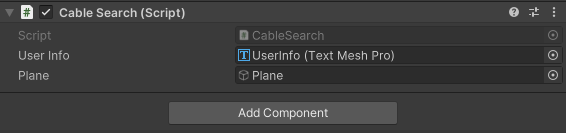
\includegraphics[scale=0.7]{images/CableSearchObjekt.png}
    \caption{\textit{Komponenten} des \textit{CableSeach} \textit{Gameobjekts}}
    \label{fig:CableSearchObjekt}
\end{figure}
Dem Skript wird zuerst ein \textit{Text Mesh Pro} übergeben, dieser Text wird innerhalb von der Unity Szene anzeigt. Sowohl wird ein weiteres \textit{Gameojekt} mit den Namen \textit{Plane} (welches ebenfalls in der Szene existiert) fürs Debuggen (Siehe Kapitel \ref{sec:PlaneDebug}) und ausführen vom weiteren Code übergeben.
\begin{lstlisting}[style=csharp, caption={Start des \textit{CableSearch} Skripts}, label=code:CableSearch]
void Start() {
    userInfo.text = "Schauen Sie auf das Rote Kabel";
    StartCoroutine(DelayedStart());
}

private IEnumerator DelayedStart() {
    yield return new WaitForSeconds(2.0f);
    canStartScript = true;
}
\end{lstlisting}
Beim Start des Skripts wird die Funktion \textit{Start} aufgerufen. Diese modifiziert den Text von \textit{userInfo}, welcher dem Benutzer angezeigt wird. Nach dieser Änderung wird eine \textit{Coroutine}, (siehe Kapitel \ref{sec:Coroutines}) gestartet und an einen neuen Thread namens \textit{DelayedStart} übergeben. Die Funktion \textit{DelayedStart} stellt sicher, dass der Benutzer die Nachricht zwei Sekunden lang lesen kann, bevor sie durch einen Timer ersetzt wird. Dieser Timer wird in der \textit{Update}-Funktion von Unity verarbeitet, um eine zeitgesteuerte Aktualisierung zu gewährleisten.
\begin{lstlisting}[style=csharp, caption={Update des \textit{CableSearch} Skripts}, label=code:Timer]
void Update() {
    /* Ueberprueft, ob das Skript gestartet werden kann und ob das Skript noch schon ausgeführt wurde*/
    if (canStartScript && !objectPlaced) {
        /* Ueberprueft ob noch Zeit uebrig ist */
        if (timeRemaining > 1f) {
            /* Verringert die verbleibende Zeit basierend auf der verstrichenen Zeit seit dem letzten Update */
            timeRemaining -= Time.deltaTime;
            /* Berechnet die verstrichene Zeit in Sekunden */
            int elapsedTime = Mathf.FloorToInt(timeRemaining % 60);
            /* Aktualisiert den Text auf dem Bildschirm mit der verbleibenden Zeit */
            userInfo.text = elapsedTime.ToString();
        }
        else {
            /* Setzt die verbleibende Zeit auf 1 Sekunde, um zu verhindern, dass sie negativ wird */
            timeRemaining = 1f;
            /* Leert den Text auf dem Bildschirm */
            userInfo.text = "";
            /* wird auf true gesetzt um zu verhindern das weiter ueberpueft wird
            objectPlaced = true;
            /* fuert den weiteren code aus */
            startPictureTaking();
        }
    }
}
\end{lstlisting}
Nach Ablauf der Wartezeit von zwei Sekunden wird eine Zeitmessung gestartet. Dabei wird zunächst geprüft, ob die Restzeit \textit{timeRemaining} (die außerhalb der Funktion als Gleitkommazahl von sechs definiert ist), größer als eins ist. Ist diese Bedingung erfüllt, wird die Restzeit durch Abziehen der verstrichenen Zeit zwischen den \textit{Updates} angepasst. Anschließend wird die verbleibende Zeit in Sekunden umgerechnet und dem Benutzer angezeigt.Nach Ablauf der fünf Sekunden Ladezeit wird die verbleibende Zeit auf eins gesetzt, um Fehler zu vermeiden. Danach wird der Text geleert und der boolesche Wert \textit{objectPlaced} auf \textit{true} gesetzt, um sicherzustellen, dass die Update-Funktion nicht weiter ausgeführt wird. Schließlich wird innerhalb der Funktion \textit{startPictureTaking} das nächste Skript gestartet, um den Prozess fortzusetzen.

\subsection{Foto aufnahme und verarbeitung}
Dieses Kapitel beschäftigt sich mit dem aufnehmen und verarbeiten von dem Foto des Roten Kabels
\subsubsection{\label{sec:Photocapture}Photocapture Klasse}
Die \textit{PhotoCapture} Klasse benutzt die \textit{PhotoCapture} API, um ein Foto mit der Kamera des Gerätes zu machen.
Damit dies möglich ist, muss man Unity die Erlaubnis für die \textit{Webcam} und das \textit{Microphone} geben. Dies gibt dann die Erlaubnis das wenn zum Beispiel ein Laptop verwendet wird. Dieser über Unity code Photos/Videos sowie Sprachaufnahmen über die Kamera und Mikrophone aufnehmen kann. Dies trifft dann natürlich auch auf die Hololens 2 zu.
Dies kann unter \textit{Edit $\Rightarrow$ Project Settings $\Rightarrow$ Player $\Rightarrow$ Settings for Universal Windows Platform $Rightarrow$ Publishing Settings $\Rightarrow$ Capabilities} gemacht werden.

Die wichtigsten Funktionen von \textit{PhotoCapture} sind:


\begin{itemize}
    \item \textbf{PhotoCapture.CreateAsync():} Erstellt asynchron eine Instanz eines PhotoCapture Objekts welches benutzt werden kann um ein Photo zu schießen.
    \item \textbf{PhotoCapture.StartPhotoModeAsync(CameraParameter):} Dafür werden die Parameter der Kamera benötigt, die zur \textit{CameraParameter}-Klasse instanziiert werden.
    \item \textbf{PhotoCapture.TakePhotoAsync():} Macht das Foto.
    \item \textbf{PhotoCaptureFrame.UploadImageDataToTexture:} Kopiert das unverarbeitete Foto innerhalb eine variable.
    \item \textbf{PhotoCaptureObject.StopPhotoModeAsync():} Beendet die Instanz des Photocapture und ruft danach die Funktion innerhalb der Klammer auf.
\end{itemize}

\subsubsection{Unity Canvas}
Ein Canvas stellt einen Bereich dar, in dem alle Benutzeroberflächen (kurz UI) enthalten sind. Die Hierarchie von so einen UI besteht aus dem \textit{GameObject} als sogenannten \textit{parent} weleches als \textit{child} die \textit{UI} besitzt. Diese \textit{UI} kann auch als weiteres child ein \textit{Image} besitzten. Das Canvas wird als Rechteck dargestellt, was es erleichtert, die genaue Position des Objekts zu bestimmen.\\
Ein Canvas verfügt auch über verschiedene Rendermodi:
\begin{itemize}

    \item\textbf{Screen Space-Overlay}: Dieser Modus ermöglicht es UI-Elementen, über der Szene auf dem Bildschirm gerendert zu werden. Das bedeutet, dass das UI-Element unabhängig von dem, was in der Szene passiert, über der Szene gerendert wird.

    \item\textbf{Screen Space-Camera}: Dieser Modus funktioniert ähnlich wie \textit{Screen Space-Overlay}, mit dem Unterschied, dass das UI-Element vor der zugewiesenen Kamera platziert wird.

    \item\textbf{World Space}: Dieser Rendermodus wird in diesem Projekt am häufigsten verwendet. In diesem Modus kann der Canvas im Gegensatz zu den anderen Modi verschoben werden, genau wie alle anderen Objekte in der Szene.\protect\footnote{Unity \cite{Canvas}}
\end{itemize}

\subsubsection{Foto der Umgebung aufnehmen}
Das Aufnehmen des Fotos wird mit Hilfe der \textit{PhotoCapture}-Klasse (siehe Kapitel \ref{sec:Photocapture}) aufgenommen wird. Um zu gewährleisten das es funktioniert und mit der Kamera ein qualitativ gutes Foto zum verarbeiten gemacht wird müssen Einstellungen der für die Kameraparameter eingestellt werden.
\begin{lstlisting}[style=csharp, caption={Bild einstellung und aufnahme}, label=code:takingPicture]
public void takingPicture() {
    // ueberprueft, ob bereits ein Bild aufgenommen wird, um zu verhindern, dass die Methode erneut aufgerufen wird
    if (!takingNewPicture) {
        // Aktiviert das LoadingSymbol-Spielobjekt, um anzuzeigen, dass ein Bild aufgenommen wird
        loadingCircle.SetActive(true);
        // Holt sich das Canvas-Objekt innerhalb des LoadingSymbol-Spielobjekts
        loadingCircleCanvas = loadingCircle.GetComponentInChildren<Canvas>();
        // Startet die Ladeanimation im LoadingCircle
        loadingCircleCanvas.GetComponent<LoadingCircle>().StartLoading();
        // Erstellt asynchron eine Fotoaufnahme
        PhotoCapture.CreateAsync(false, delegate (PhotoCapture captureObject) {
            // ueberprueft, ob die Fotoaufnahme erfolgreich erstellt wurde
            if (captureObject != null) {
                // Speichert die Fotoaufnahme in einer Instanzvariablen
                photoCaptureObject = captureObject;
                // Konfiguriert die Kameraparameter fuer die Aufnahme
                CameraParameters cameraParameters = new CameraParameters();
                cameraParameters.hologramOpacity = 0.0f;
                // Setzt die Aufloesung der Kamera
                cameraParameters.cameraResolutionWidth = cameraResolution.width;
                cameraParameters.cameraResolutionHeight = cameraResolution.height;
                // Setzt das Pixelformat fuer die Aufnahme
                cameraParameters.pixelFormat = CapturePixelFormat.BGRA32;
                try {
                    // Startet asynchron den Fotoaufnahmemodus
                    photoCaptureObject.StartPhotoModeAsync(cameraParameters, delegate (PhotoCapture.PhotoCaptureResult result) {
                        // Nimmt ein Foto auf und speichert es im Arbeitsspeicher
                        photoCaptureObject.TakePhotoAsync(onCapturedPhotoToMemory);
                    });
                }
            }
        });
    }
}
\end{lstlisting}
Zunächst wird in diesem Code mit dem Boolean \textit{takingNewPicture} geprüft, ob bereits ein Bild aufgenommen wurde. Daraufhin wird sofort das Lade-Symbol (siehe Kapitel \ref{sec:ladeSymbol}) gestartet und angezeigt. Anschließend wird eine asynchrone Methode \textit{PhotoCapture.CreateAsync()} aufgerufen, um ein \textit{Photo-Capture} zu erstellen. Diese Methode erstellt ein \textit{PhotoCapture-Objekt}, das für die Aufnahme von Fotos verwendet wird. Die Methode akzeptiert den Parameter false, der angibt, dass kein Audio-Capture erstellt werden soll. Wenn die Aufnahme erfolgreich war, wird das PhotoCapture-Objekt gespeichert und die Kameraparameter für die Aufnahme konfiguriert. Anschließend wird der Photo-Capture-Modus mit \textit{StartPhotoModeAsync} gestartet, und wenn dieser erfolgreich gestartet wurde, wird das Photo aufgenommen und mit \textit{TakePhotoAsync} im Speicher abgelegt.

\subsubsection{\label{sec:JobSystem}Unity Job System}
Das Job System von Unity bietet eine effiziente Möglichkeit zur Implementierung von Multithreading in Anwendungen, wodurch die Anwendung in
der Lage ist, alle verfügbaren CPU-Kerne optimal zu nutzen. Im Gegensatz zu einem sequentiellen Durchlauf des Codes durch einen einzigen Thread, dem sogenannten Hauptthread, ermöglicht das Job System die parallele Verarbeitung von Codeabschnitten durch separate Arbeits-Threads. Durch die Nutzung mehrerer Arbeits-Threads können Aufgaben effizienter verteilt und gleichzeitig bearbeitet werden. Dies trägt wesentlich zur Verbesserung der Effizienz und der Gesamtdauer der Ausführung des Programms bei. Eine wichtige Eigenschaft des Job Systems besteht darin, sicherzustellen, dass nur so viele Threads verwendet werden, wie von den verfügbaren CPU-Kernen unterstützt werden.\\
Ein weiteres wichtiges Konzept, das im Job System implementiert ist, ist das sogenannte "Work Stealing". Dabei handelt es sich um eine Planungsstrategie für Threads, bei der ein Thread, der seine aktuellen Aufgaben abgeschlossen hat, zusätzliche Aufgaben von anderen Arbeits-Threads übernimmt und sie in seine eigene Warteschlange einfügt. Dies ermöglicht eine dynamische und effiziente Verteilung von Aufgaben zwischen den Threads und trägt dazu bei, die Last gleichmäßig auf alle verfügbaren Ressourcen zu verteilen. \\
Um das Schreiben von Multithread-Code zu erleichtern, verfügt das Job-System über ein Sicherheitssystem, das sicherstellt, dass potenzielle Wettlaufbedingungen eine sogenannte \textit{race contition} zu vermieden und somit Fehler vermieden werden können. Um sicherzustellen, dass keine Wettlaufbedingungen auftreten können, erhält jeder Thread eine isolierte Kopie der Daten, die er verarbeiten kann.\protect\footnote{Unity \cite{Job System}}


\subsubsection{\label{sec:Vector2}Vector2 Klasse}
Unity bietet dem Benutzer eine umfassende Funktionalität zur Darstellung und Manipulation von 2D-Positionen, -Richtungen und -Geschwindigkeiten innerhalb deren \textit{Engine}. Mit Hilfe der \textit{Vektor2D} klasse von Unity lassen sich Bewegung, Interaktion und Objekte exakt steuern und simulieren. Diese Klasse besitzt die folgenden Parameter:
\begin{itemize}
    \item \textit{x und y: }x Koordinate von einen 2 Dimensionalen Koordinatensystem
    \item \textit{magnitude: }Besitzt die größe des 2D Vektors. Die größe wird des Vektors wird mithilfe von dieser Formel berechnet $\sqrt{x^2 + y^2}$
    \item \textit{normalized: }Normalisierung bedeutet, den Vektor auf eine Länge von 1 zu bringen, während seine Richtung beibehalten wird.
\end{itemize}

\subsubsection{Fotoverarbeitung}
Nachdem ein Foto aufgenommen wurde, erfolgt die Datenverarbeitung mittels einer \textit{Texture2D}-Klasse innerhalb des \textit{Unity-Job-Systems} in paralleler Ausführung. Jeder Thread des Systems ist dafür zuständig, eine festgelegte Anzahl von Pixeln im Bild zu überprüfen, um festzustellen, ob diese die Eigenschaft Rot aufweisen. Die Ergebnisse dieser Überprüfung werden in einem zweidimensionalen Boolean-Array gespeichert, wobei die x- und y-Koordinaten jeweils einer Dimension zugeordnet sind. Jeder Pixel im Array wird entsprechend seines Farbzustands mit dem booleschen Wert \textit{true} gekennzeichnet, falls er rot ist, andernfalls wird ihm der Wert \textit{false} zugewiesen. Dieser Prozess wird durch das \textit{Job-System} ausgeführt, wobei jeder einzelne Job die eine gewisse Anzahl an Pixeln überprüft.

\begin{lstlisting}[style=csharp, caption={Rote Pixel suche}, label=code:PixelJob]
struct PixelJob : IJobParallelFor {
    public NativeArray<Color> pixels;
    public NativeArray<Vector2> redPixelPositions;
    public int textureWidth;
    public int batchSize;

    public void Execute(int batchIndex) {
        int startPixelIndex = batchIndex * batchSize;
        int endPixelIndex = Mathf.Min((batchIndex + 1)
        * batchSize, pixels.Length);

        for (int pixelIndex = startPixelIndex;
        pixelIndex < endPixelIndex; pixelIndex++) {
            int x = pixelIndex % textureWidth;
            int y = pixelIndex / textureWidth;

            if (pixels[pixelIndex].r > 0.7f &&
            pixels[pixelIndex].g < 0.5f && pixels[pixelIndex].b < 0.5f) {
                pixels[pixelIndex] = Color.red;
                redPixelPositions[pixelIndex] = new Vector2Int(x, y);
            }
            else {
                pixels[pixelIndex] = Color.black;
            }
        }
    }
}
\end{lstlisting}
\begin{itemize}
    \item \textbf{NativeArray:} bieten verbesserte Leistung im Vergleich zu standardmäßige Arrays, da diese direkt auf native Speicherbereiche zugreifen können, was besonders wichtig ist, wenn große Datenmengen verarbeitet werden müssen und die Ausführung parallelisiert werden soll.
    \item \textbf{pixels:} pixels ist ein \textit{NativeArray} welcher die aktuell noch unbearbeiteten Pixels beinhaltend.
    \item \textbf{batchSize:} Die \textit{batchSize} beinhaltet die Anzahl von Pixel die jeder \textit{Job} durchgeht und überprüft.
    \item \textbf{texturewidth:} Wird vor dem Aufruf der \textit{Jobs} berechnet um die Koordinaten des roten Pixels herauszufinden.
    \item \textbf{batchIndex:} Nachdem der Prozess unter mehreren \textit{Jobs} aufgeteilt wird und alle \textit{Jobs} von an den selben \textit{NativeArray} \textit{pixels} arbeiten. Bekommt jeder \textit{Job} einen \textit{batchIndex} mit, dieser zeigt an wo die Arbeit dieses \textit{Jobs} innerhalb des \textit{NativeArray} beginnt.
    \item \textbf{startPixelIndex:} nachdem jeder Arbeiter Thread seine eigenen Batches Besitz muss der Index für diese berechnet werde.
    \item \textbf{redPixelPositions:} Wird vor der Initialisierung in der Klasse mit der selben Länge wie Pixels erstellt.
\end{itemize}


\subsubsection{Kabel finden}
Nachdem das Foto verarbeitet wurde wird nach roten Pixel in dem Bild gesucht, um danach die noch fehlende Entfernung des Kabels zu messen. Mit dieser hat man dann die genaue Position des roten Kabels in der Echten Welt errechnet. Um dies zu erreichen wird nach roten Objekten Roten Pixeln im Bild gesucht. Da es aber unsicher ist, ob diese roten Pixel zu einem Kabel gehören oder nicht, wird eine Methode angewendet, um die längste zusammenhängende Reihe von roten Pixeln zu ermitteln. Es kann auch dazu kommen, das rote Pixel nicht erkannt werden ,welche zum roten Kabel gehören. Aus diesem Grund wird ein Toleranzbereich festgelegt. Es wird geschaut ob in einen bestimmten Bereich rote Pixel existieren von welchen aus dann weiter geschaut wird. Dadurch wird eine präzisere Erkennung und Zuordnung von relevanten roten Pixeln im Kontext des zu identifizierenden Kabels ermöglicht. Die methodische Vorgehensweise zur Berechnung gestaltet sich wie folgt:

\begin{lstlisting}[style=csharp, caption={Kabel suche}, label=code:SearchForRedPixels]
List<Vector2> SearchForRedPixels(int startX, int startY) {
        /* Ist die momentane Line an der er Schaut ob sie einen weiteren Punkt findet */
        List<Vector2> currentLine = new List<Vector2>();
        bool hasFound = false;
        /* foundX und foundY sind die momentare x und y positionen des Roten pixels von den man ausgeht */
        int foundX = startX, foundY = startY;
        /* heightY wird verwendet um zu ueberpruefen ob die gepruefte laenge nicht die exestierente uebertrifft */
        int heightY = redPixels.GetLength(1);
        /* withX wird verwendet um zu ueberpruefen ob die gepruefte breite nicht die exestierente uebertrifft */
        int withX = redPixels.GetLength(0);

        do {
            hasFound = false;
            /* Damit die funktion nicht in eine unendlich schleife bei den darueber und darunter ueberpruefen kommt wird die Position von redPixels auf false gesetzt*/
            redPixels[foundX, foundY] = false;
            currentLine.Add(new Vector2(foundX, foundY));
            /* ueberprueft ob 25 pixel "rechts" von den Pixel von den man ausgehen mindestens ein roter vorhanden ist */
            for (int i = 1; i < 25 && foundX + i < withX; i++) {
                if (redPixels[foundX + i, foundY]) {
                    foundX = foundX + i;
                    hasFound = true;
                }
            }

            /* ueberprueft ob 10 pixel "unter" von den Pixel von den man ausgehen mindestens ein roter vorhanden ist */
            for (int i = 1; i < 10 && !hasFound && foundY - i > 0; i++) {
                hasFound = redPixels[foundX, foundY - i];
                if (hasFound) {
                    foundY = foundY - i;
                }
            }

            /* ueberprueft ob 10 pixel "ueber" von den Pixel von den man ausgehen ueberprueft ein roter vorhanden ist */
            for (int i = 1; i < 10 && !hasFound && foundY + i < heightY; i++) {
                hasFound = redPixels[foundX, foundY + i];
                if (hasFound) {
                    foundY = foundY + i;
                }
            }
        } while (hasFound);
        return currentLine;
    }
\end{lstlisting}
Die Funktion beginnt mit der Erstellung einer Liste von Vektoren namens \textit{currentLine}, die dazu dient, die Positionen der gefundenen Pixel zu speichern. Zu Beginn wird festgelegt, dass kein rotes Pixel gefunden wurde (\textit{hasFound = false}). Die x- und y-Positionen des Startpixels werden ebenfalls initialisiert (\textit{foundX = startX, foundY = startY}). Zudem werden Variablen für die Höhe (\textit{heightY}) und Breite (\textit{withX}) des Arrays \textit{redPixels} festgelegt, um sicherzustellen, dass die Überprüfungen nicht außerhalb des gültigen Bereichs liegen. Der Hauptteil der Funktion ist eine Schleife, die so lange ausgeführt wird, bis kein rotes Pixel mehr gefunden wird. Innerhalb dieser Schleife wird zuerst das aktuelle Pixel als bereits überprüft markiert und seiner Position zur Liste \textit{currentLine} hinzugefügt. Anschließend wird nach roten Pixeln in den nächsten 25 Pixeln nach rechts gesucht. Dabei wird überprüft, ob das Pixel in \textit{redPixels} an der Position \textit{(foundX + i, foundY)} den Wert \textit{true} hat, wobei \textit{i} von 1 bis 24 läuft. Wenn ein rotes Pixel gefunden wird, wird dessen Position aktualisiert und die Schleife erneut durchlaufen. Falls kein rotes Pixel in den nächsten 25 Pixeln nach rechts gefunden wird, wird nach unten und dann nach oben gesucht. Dabei wird jeweils überprüft, ob in den nächsten 10 Pixeln in der entsprechenden Richtung ein rotes Pixel vorhanden ist. Wenn eins gefunden wird, wird dessen Position aktualisiert und die Schleife erneut durchlaufen. Diese Schleife setzt sich solange fort, bis kein rotes Pixel mehr gefunden wird (\textit{hasFound = false}). Schließlich wird die Liste \textit{currentLine}, die die Positionen der gefundenen Pixel enthält, zurückgegeben.


\subsection{\label{sec:Coroutines}Coroutines}
\textit{Coroutines} werden immer noch mit den Mainthread ausgeführt, erlaube es den für \textit{Coroutines} verwendeten Code über mehrere Frames aufzuteilen. \textit{Coroutines} weden deswegen hauptsächlich in Methoden verwendet welche eine Abfolge von Ereignissen über zeit darstellt.
\\
Zum Darstellen von \textit{Coroutines} ist dieses kurze Script welches das Objekt an den das angebunden ist in eine Richtung bewegt.
\begin{lstlisting}[style=csharp, caption={Coroutine Beispiel}, label={code:coroutineBsp}]
public class CoroutineExample : MonoBehaviour {
    // Das Zielobjekt, zu dem das Objekt bewegt werden soll
    public Transform target;
    // Die Geschwindigkeit, mit der das Objekt bewegt wird
    public float moveSpeed = 1f;
    // Die Anzahl der Schritte für die Bewegung
    public int numSteps = 10;

    void Start() {
    // Starte die Coroutine für die Bewegung
        StartCoroutine(MoveToTarget());
    }

    IEnumerator MoveToTarget() {
    // Die Startposition des Objekts
        Vector3 startPos = transform.position;
        // Die Zielposition des Objekts
        Vector3 endPos = target.position;
        // Iteriere ueber jeden Schritt der Bewegung
        for (int i = 0; i <= numSteps; i++) {
            // Berechne den Fortschritt der Bewegung (Wert zwischen 0 und 1)
            float t = (float)i / numSteps;
            // Bewege das Objekt entsprechend dem aktuellen Fortschritt
            transform.position = Vector3.Lerp(startPos, endPos, t);
            // Wartet fuer eine bestimmte Zeit, bevor der nächste Schritt ausgefuehrt wird
            yield return new WaitForSeconds(moveSpeed / numSteps);
        }
    }
}
\end{lstlisting}
Wenn dieses Skript zu einem \textit{GameObject} hinzugefügt wird, bewegt sich das Objekt mit der angegebenen Geschwindigkeit. Diese Geschwindigkeit gibt die variable \textit{moveSpeed} an, welches wenn nichts angegeben wird, standardmäßig auf eins gesetzt wird. Es wird auch angegeben in wie vielen Schritten (also Frame-Passagen) der Vorgang stattfinden soll, dies übernimmt die variable \textit{numSteps}. Dann soll auch noch die Position, wo das Objekt am Ende ankommen soll als \textit{Transform} mit dem Namen \textit{target} angegeben werden. Die \textit{Transform} Klasse welche speichert die Position, Rotation und Größe und lässt diese auch bearbeitet. \\
Beim Start des Skripts wird sofort die \textit{Courutine} mit der von Unity zur Verfügung gestellten \textit{StartCoroutine} mit der entsprechenden \textit{IEnumerator} Funktion innerhalb der Klammern aufgerufen. Die Funktion \textit{MoveToTarget} muss mit der Klasse \textit{IEnumerator} geschrieben werden, da wenn es ohne der \textit{IEnumerator} Klasse nicht möglich wäre, die Methode \textit{MoveToTarget} als Coroutine zu verwenden und mit \textit{StartCoroutine} aufzurufen. \textit{Coroutine}-Funktionen müssen eine \textit{IEnumerator}-Rückgabe haben, damit Unity sie als asynchrone Task ausführen kann. Durch die Verwendung von \textit{IEnumerator} können innerhalb von \textit{Coroutine} \textit{yield}-Anweisungen verwendet werden, um zu steuern, wann und wie die Ausführung unterbrochen und fortgesetzt wird. In diesem Beispiel wird \textit{yield return new WaitForSeconds(moveSpeed / numSteps)} verwendet, um zwischen den einzelnen Schritten der Bewegung eine Pause einzulegen, bevor der nächste Schritt im nächsten Frame ausgeführt wird. Dies ermöglicht eine fließende und kontrollierte Bewegung des Objekts. \\
\\
Falls man aus irgendeinen Grund so eine Coroutine beenden will kann man auch \textit{StopCoroutine} oder \textit{StopAllCoroutines} verweden. Als Beispiel wird eine sehr kleine Erweiterung von den Code Abschnitt \ref{code:coroutineBsp}.
\begin{lstlisting}[style=csharp, caption={Coroutine beenden}, label=code:debugRaycast]
public void stopFunctionCoroutine() {
    StopCoroutine(MoveToTarget)
}

public void stopAllCurrentCoroutine() {
    StopAllCoroutines()
}
\end{lstlisting}
\begin{itemize}
    \item StopCoroutine: Sorgt dafür das nur die \textit{IEnumerator} Funktion welche für die \textit{Coroutine} verwendet wurde beendet wird.
    \item StopAllCoroutine: Sorgt dafür das alle Funktion welche für alle laufenden \textit{Coroutine} verwendet wurde beendet werden.
\end{itemize}

\subsection{Lade Symbol}\label{sec:ladeSymbol}
Das Lade Symbol ist eine visuelle Darstellung, die den Benutzer darüber informiert, dass Berechnungen oder Prozesse im Hintergrund ausgeführt werden. In erster Linie wird dieses Symbol während der Kabelsuche verwendet. Diese Animation des Lade Symbols wird durch entsprechenden Programmcode gesteuert, um dem Benutzer eine klare und konsistente Rückmeldung zu geben, dass der Prozess läuft. Im Design der Interaktion spielt das Ladesymbol eine wichtige Rolle, um den Benutzer über den aktuellen Status der Anwendung zu informieren.
\begin{figure}[H]
    \centering
    \begin{minipage}[b]{0.65\textwidth}
        \centering
        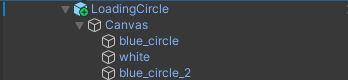
\includegraphics[width=\textwidth]{images/LadeKreisHierachy.png}
        \caption{Hierarchie Lade Kreises im Unity Editor}
    \end{minipage}
    \hfill
    \begin{minipage}[b]{0.3\textwidth}
        \centering
        
\includegraphics[width=\textwidth]{images/LadeKreisBsp.png}
        \caption{Lade Symbol}
        \label{fig:Loading}
    \end{minipage}
\end{figure}
\begin{lstlisting}[style=csharp, caption={Code zum ausführen des lade Symbols}, label=code:LoadingCoroutine]
IEnumerator LoadingCoroutine() {
    while (isRunnig) {
        if (img.fillAmount >= 1f) {
            img.fillAmount = 0f;
        }
        else {
            img.fillAmount += fillSpeed;
        }
        yield return new WaitForSeconds(0.1f);
    }
}
\end{lstlisting}
Um eine Funktion in einem parallelen Thread auszuführen, während der Hauptthread gleichzeitig Berechnungen durchführt, ist es erforderlich, eine Funktion in einen separaten Thread auszulagern. Dies wird in den fall durch die Verwendung von Asynchronität erreicht. Dafür gibt Unity die Funktion Coroutine-Routinen zur Verfügung. Bei der Initiierung dieser Funktion wird die Methode \textit{StartCoroutine(LoadingCoroutine())} aufgerufen. Durch diesen Aufruf wird sichergestellt, dass die Funktion nebenbei und asynchron zum Code davor(main thread) ausgeführt wird. Zum anzeigen von den Lade Symbol wird ein Objekt \textit{img} verwendet, dieses \textit{img} beinhaltet ein Bild eines Weißen Kreises (äußerer Kreis von \textit{Abbildung (\ref{fig:Loading}})) und stellt den Fortschritt während der Berechnung dar.


\subsection{Bewegung des Paketes}
Um das Paket über das Kabel gleiten zu lassen, muss zuerst der Abstand gemessen werden. Sobald diese gemessen wurde, sind alle wichtigen Punkte berechnet, über die das Paket gleiten soll. Dann muss das Objekt, welches das Paket darstellt, initialisiert und am Anfang des Kabels positioniert werden. Danach wird sich das Paket über die Punkte bewegt.
\subsubsection*{Definition eines Rays}
Ein Ray ist ein abstraktes Konzept in der Computergrafik und Physiksimulation, das einen unendlich langen, geraden Strahl repräsentiert. Dieser Strahl wird durch einen Ausgangspunkt definiert, der üblicherweise als \textit{Ursprung} bezeichnet wird. Im Kontext von dreidimensionalen Szenen und Visualisierungen entspricht der Ursprung oft der Position einer \textit{virtuellen Kamera} oder eines \textit{Blickpunkts}. Der Ray erstreckt sich dann in eine bestimmte Richtung, die durch Vektor definiert wird. Diese Richtung kann durch verschiedene Methoden festgelegt werden, abhängig von der Anwendung, in der der Ray verwendet wird. Im Falle der Bildschirmkoordinaten kann die Richtung beispielsweise durch  Blick des Benutzers bestimmt werden. In der Praxis wird der Ray häufig dazu verwendet, um \textit{Kollisionen mit Objekten in einer Szene zu erkennen} oder \textit{um Lichtstrahlen für die Beleuchtungsberechnung zu simulieren}. Durch das Schießen eines Rays in eine Szene und das Überprüfen auf \textit{Kollisionen} mit den vorhandenen Objekten kann festgestellt werden, ob der Ray ein Objekt trifft und wenn ja, an welcher \textit{Stelle} und unter welchem \textit{Winkel}.\\

\subsubsection{\label{sec:ARRaycastHit}ARRaycastHit Klasse}
Die \textit{ARRaycastHit} Klasse in Unity wird verwendet, um die Ergebnisse eines \textit{Raycasts} in Augmented Reality (AR) Anwendungen zu erhalten. Ein Raycast ist eine Technik, bei der ein imaginärer Strahl (Ray) von einem Startpunkt aus in eine bestimmte Richtung gesendet wird, um festzustellen, ob er auf eine Oberfläche auftrifft, und, wenn dies der Fall ist, Informationen über den Auftreffpunkt zurückzugeben. Diese Informationen werden dann von der \textit{ARRaycastHit}-Klasse aufgefangen und zur Verfügung gestellt.Die \textit{ARRaycastHit}-Klasse enthält mehrere Methoden, die es ermöglichen, auf die Details des Treffpunkts zuzugreifen und entsprechende Aktionen in einer AR-Anwendung auszuführen. Dazu gehören Informationen wie die Position des Trefferpunktes, die Entfernung zum Startpunkt des Strahls. Durch die Verwendung der \textit{ARRaycastHit}-Klasse ist es möglich, präzise Interaktionen in AR-Szenen zu implementieren, wie z.B. das Platzieren virtueller Objekte auf realen Oberflächen. Darüber hinaus ermöglicht die \textit{ARRaycastHit}-Klasse das Hinzufügen von physikalischen Eigenschaften in AR-Anwendungen, wodurch z. B. Kollisionen integriert werden können.
Diese Klasse besitzt die folgenden Parameter:
\begin{itemize}
    \item \textit{hit: } \textit{hit} ist eine \textit{XRRaycastHit}-Klasse welche die unverarbeiteten Daten von den \textit{hit} beinhaltet.
    \item \textit{distance: } Enthält die Entfernung vom Ursprung des Strahls bis zu dem Punkt, an dem er getroffen wurde.
    \item \textit{hitType: } Trefferart, die angibt, ob der Strahl einen Punkt (Feature Point) oder ein Objekt (Trackable) getroffen hat.
\end{itemize}

\subsubsection{Entfernung messen}
Da man noch die z-Achse, also die Tiefe, ermitteln muss, um das visuelle Paket angemessen auf dem (physischen) zu platzieren und bewegen zu können, werden
im späteren Verlauf RayCasts\protect\footnote{Unity \cite{Raycast}} verwendet. Aufgrund der Ressourcenintensität, die mit dem Versenden eines Raycasts
für jede Position verbunden wäre, um die z-Achse für jede x/y Koordinate zu erhalten, ist eine Optimierung notwendig.
Zur Verbesserung der Effizienz werden die wichtigsten Positionen berechnet. Diese wichtigen Punkte sind der
Anfangspunkt des Kabels (am ersten PC), der Mittelpunkt des Kabels, der Endpunkt des Kabels (am zweiten PC), sowie zehn andere Punkte welche gleichmäßig über das gesamte Kabel verteilt sind. Diese Punkte werden in einer globalen \textit{List<Vector3>} Variable namens \textit{redPixelCoordinates} gespeichert um auf alle 3 Koordinaten (x/y/z) zugreifen zu können. Diese Liste wird durch Iterieren und für jeden Punkt wird ein Raycast ausgeführt.
\begin{lstlisting}[style=csharp, caption={Iteration durch die Liste der Raycastpunkte}, label=code:]
foreach (Vector2 redPixle in redPixelCoordinates) {
    positionVirtualObject(redPixle, targetTexture)
}
\end{lstlisting}
\begin{itemize}
    \item \textit{positionVirtualObject} ist die Funktion welche die folgenden Berechnungen für Raycasts errechnet und den Raycast ausführt. \\
\end{itemize}
Um Raycasts erfolgreich zu nutzen, greift Unity auf Bildschirmkoordinaten zurück. Jedoch liegen uns momentan nur die Koordinaten vor, die der Skalierung des Bildes entsprechen. Daher müssen diese in ein Format umgerechnet werden, das es ermöglicht, die Raycasts an die richtigen Positionen zu senden. Diese Umrechnung erfolgt im Code wie folgt:
\begin{lstlisting}[style=csharp, caption={Koordinaten Umrechnung}, label=code:Coordinates calculations]
Vector2 screenCoordinates = new Vector2(
    redPixel.x * Camera.main.pixelWidth / image.width,
    redPixel.y * Camera.main.pixelHeight / image.height
);
\end{lstlisting}

\begin{itemize}
    \item \textbf{redPixel.x} und \textbf{redPixel.y} sind die Positionen welche in \textit{screenCoordinates} umgerechnet werden soll.
    \item \textbf{Camera.main.pixelWidth} und \textbf{Camera.main.pixelHeight} sind die Breite und Höhe des Bildschirms, auf dem die Kameraansicht dargestellt wird.
    \item \textbf{image.width} und \textbf{image.height} sind die gesamte Breite und Höhe des verarbeiteten Bildes vom roten Kabel in Pixels.
\end{itemize}
Sobalt dann die \textit{screenCoordinates} berechnet wurden, wird der Raycast auf die Position im Bildschirm aufgerufen werden. Dafür ist dieser Code teil von \textit{positionVirtualObject} zuständig:
\begin{lstlisting}[style=csharp, caption={Raycast schießen}, label=code:createRaycast]
List<ARRaycastHit> hits = new List<ARRaycastHit>();
if (raycastManager.Raycast(screenCoordinates, hits, TrackableType.Planes)) {
    for (int i = 0; i < hits.Count; i++) {
        if (hits[i].hitType != TrackableType.PlaneWithinInfinity) {
            if (hits[i] != null) {
                cablePositinos.Add(new Vector3(hits[i].pose.position.x, hits[i].pose.position.y + 0.05f, hits[i].pose.position.z));
                break;
            }
        }
    }
}
\end{lstlisting}
Es wird eine Liste von ARRaycastHit Objekten erstellt, die den Namen \textit{hits} trägt. In dieser Liste werden nach dem Ausführen einer AR-Raycast-Operation die Treffer gespeichert. Die Funktion Raycast erhält die \textit{screenCoordinates}, die \textit{hits}-Liste sowie die zu suchenden TrackableType.Planes.
Wenn die Funktion mindestens einen Treffer erhält, werden alle Treffer überprüft. Diese Treffer werden dann daraufhin überprüft, ob ihr Typ nicht \textit{TrackableType.PlaneWithinInfinity} ist, um sicherzustellen, dass der Raycast nicht ins Unendliche geht. Wenn ein Objekt getroffen wurde, wird geprüft, ob es Werte besitzt. Wenn alle diese Voraussetzungen erfüllt sind, wird es mit einer um 5 cm erhöhten Höhe (damit das Paket nicht innerhalb von Kabel gleitet sondern leicht darüber) zu \textit{cablePositions} hinzugefügt. \textit{cablePositions} ist die Position, die das Paket später durchqueren wird.

\subsubsection{Erstellung und Positionierung des Paketes}
Nach der Bestimmung der kritischen Positionen mittels Raycast hat der Benutzer die Möglichkeit, über die Website eine Nachricht zu übermitteln. Die Übermittlung dieser Nachricht löst ein entsprechendes Ereignis aus, das zur Initialisierung und zum Absenden des Datenpakets führt.\\
Bei der \textit{Start} Funktion welche von Unity zur Verfügung gestellt  wird. Führt diese Zeile aus:
\begin{lstlisting}[style=csharp, caption={Binden an der Methode}, label=code:]
EventManager.OnMessageReceived += editAndSendPackage;
\end{lstlisting}
Diese Zeile sorgt dafür das beim Start der Unity \textit{Scene} \textit{editAndSendPackage} an dem Event \textit{OnMessageReceived} gebunden wird. Das Bedeutet das wenn das Event \textit{OnMessageReceived} erhalten wird, wird die Funktion \textit{editAndSendPackage} ausgelöst.
Die Funktion \textit{editAndSendPackage} initialisiert das visuelle Paket am Anfang des Kabels falls es noch nicht erstellt wurde.
\begin{lstlisting}[style=csharp, caption={Initialisierung und Bearbeitung des Paketes}, label=code:editAndSendPackage]
public void editAndSendPackage(string username, string message) {
    if (isAtEnd) {
        isAtEnd = false;
        moveToCounter = 1;
        moveFromCounter = 0;
    }
    MainThreadDispatcher.Instance().Enqueue(() => {
        if (isObjectInstantiated == false) {
            instantiatedObject = Instantiate(virtualObject, cablePositinos[0], Quaternion.identity);
            isObjectInstantiated = true;
        }
        else {
            Destroy(instantiatedObject);
            instantiatedObject = Instantiate(virtualObject, cablePositinos[0], Quaternion.identity);
        }
        shouldMove = !shouldMove;
        EditTextOfInformationObject editTextOfInformationObject = new EditTextOfInformationObject(infoTextS);
        editTextOfInformationObject.GetTextMeshProFromChild();
        editTextOfInformationObject.EditText(username, message);
        EventManager.SendMsg(username, message);
    });
}
\end{lstlisting}
Im Rahmen der Methode wird zunächst geprüft, ob ein Paket erstellt wurde und ob es sich bereits am Ende des vorgesehenen Weges befindet. Sollte dies der Fall sein, wird der Zähler für die Bewegung des Paket zurückgesetzt. Aufgrund der Tatsache, dass der \textit{EventManager}, der die Funktion aufruft, nicht im Hauptthread läuft und die Initialisierung des Paket sowie die Funktion \textit{EventManager.SendMsg} nur im Hauptthread ausgeführt werden darf, ist die Verwendung des \textit{MainThreadDispatcher} erforderlich. Dieser stellt sicher, dass dieser Codeabschnitt nicht von einem Nebenthread, sondern vom Hauptthread ausgeführt wird. Dies ist notwendig, um sicherzustellen, dass die Unity-Szene synchronisiert ist, wie von Unity vorgegeben. Innerhalb des \textit{MainThreadDispatcher} wird, wenn das Objekt noch nicht erstellt wurde, dieses am Anfang des Kabels erstellt. Wenn das Paket jedoch bereits erstellt wurde, wird es zerstört und wieder auf die Startposition zurückgesetzt. Die Klasse \textit{EditTextOfInformationObject} ist dafür verantwortlich, das \textit{TextMeshPro} des Gameobjects zu verwenden, um die korrekten Daten im Text anzuzeigen.


\subsubsection{Bewegung des Paketes}
Die Bewegung des Paketes läuft so ab, dass das Paket nacheinander die Punkte durchläuft, welche davor berechnet wurden. Die Bewegung zwischen diesen Positionen wird innerhalb von Unity übver die Funktion \textit{Update} ausgeführt. Diese Funktion wird bei jeden Frame aufgerufen, um eine kontinuierliche Aktualisierung der Position des Pakets zu gewährleisten und somit eine nahtlose Bewegung darzustellen zu erzielen.
\begin{lstlisting}[style=csharp, caption={Update Funktion}, label=code:Update]
void Update() {
    if (shouldMove) {
        if (moveToCounter < cablePositinos.Count) {
            instantiatedObject.transform.Translate((cablePositinos[moveToCounter] - cablePositinos[moveFromCounter]) * 0.0075f);
            if (Vector3.Distance(instantiatedObject.transform.position, cablePositinos[moveToCounter]) < 0.00375f) {
                instantiatedObject.transform.position = cablePositinos[moveToCounter];
                moveToCounter++;
                moveFromCounter++;
                if (Vector3.Distance(instantiatedObject.transform.position, cablePositinos[cablePositinos.Count - 1]) < 0.00375f) {
                    isAtEnd = true;
                }
            }
        }
        else {
            shouldMove = false;
        }
    }
}
\end{lstlisting}
Dieses Skript beinhaltet drei Globale Variablen welche von mehreren Funktionen gebraucht werden
\begin{itemize}
    \item \textit{shouldmove} is ein Boolischer Wert (welcher wahr oder falsch sein kann.) Dieser wird verwendet um zu überprüfen ,ob das Objekt initialisiert wurde und sich bewegen sollte.
    \item \textit{moveFromCounter} ist ein Integer Wert, welcher mit zählt, wie oft das Paket schon von einer Position aus weg bewegt hat. Dieser Zähler wird als Index für die Liste \textit{cablePositions} verwendet um die momentane Position des Paketes zu finden.
    \item \textit{moveToCounter} ist genauso wie \textit{moveFromCounter} ein Integer, welcher ebenfalls als Index für die Liste \textit{cablePositions} benutzt wird um die Position zu finden wo das Paket als nächstes hin soll.
\end{itemize}
Nachdem geprüft wurde, ob sich das Objekt bewegen soll, wird weiterhin überprüft, ob die Nachricht bereits am Ende angekommen ist. Dies wird durch den Vergleich zwischen der Variable \textit{moveToCounter} und der Anzahl der Positionen in \textit{cablePositions} festgestellt. Diese Überprüfung ist erforderlich, da der Index einer Liste bei null beginnt, und eine Fortsetzung ohne diese Kontrolle zu einer möglichen Null-Exception führen würde. Solange \textit{moveToCounter} kleiner ist als die Anzahl der Positionen, wird die Bewegung mittels \textit{instantiatedObject.transform.Translate} ausgeführt. Die Bewegung selbst wird durch die Differenz der nächsten Position, zu der das Objekt bewegt werden soll, und der aktuellen Position, von der das Paket sich weg bewegt, definiert. Diese Translation wird mit einem Faktor multipliziert, in diesem Fall mit \textit{0.0075f}, um die Geschwindigkeit des Objekts anzupassen. Die Bewegung erfolgt mit einer Geschwindigkeit von 0.0075 Metern pro Frame(, da die Einheiten direkt in Metern angegeben sind). Nach jeder Bewegung wird überprüft, ob das Paket bereits den Endpunkt erreicht hat. Dieser Überprüfungsbereich umfasst die Hälfte der Geschwindigkeit, mit der sich das Objekt bewegt. Diese Wahl erfolgt, damit das Objekt nicht versehentlich über den Endpunkt hinausgeht, da es sich mit einer festen Geschwindigkeit von 0.0075 bewegt und somit mindestens um die Hälfte, also 0.00375, überprüft werden muss. Sobald sich das Objekt innerhalb dieses Bereichs befindet, wird seine Position festgelegt, um zu verhindern, dass das Paket über das Ziel hinausläuft. Anschließend wird der Bewegungszähler erhöht, und falls dies nicht der letzte Durchlauf war, wird der Vorgang wiederholt.


\subsection{Anzeigen von Informationen der Nachricht}
Der Benutzer kann Mithilfe der Website welche auf beiden Laptops (links und rechts) offen ist eine Nachricht innerhalb des Paketes senden. Diese Informationen werden dann angezeigt wenn der Benutzer auf das virtuelle Paket klickt.
%TODO Foto Informationen anzeigen
Dies wird mithilfe des Gameobjekt \textit{InfoObject} gemacht welches Voreinstellungen für den Hintergrund und Text besitzt falls es zu Fehlern kommt. \\
Um den Text des Objekts zu ändern muss auf das \textit{Text Mesh Pro} Gameobjekt welches ein unter Objekt des \textit{InfoObject} zugegriffen werden. Dies passiert durch diesen code
\begin{lstlisting}[style=csharp, caption={Kind vom Gameobjekt bekommen}, label=code:]
public class EditTextOfInformationObject : MonoBehaviour
{
    // Referenz auf das Elternspielobjekt, von dem aus das Kindspielobjekt gefunden werden soll
    public GameObject parentGameObject;
    // Referenz auf das TextMeshPro-Objekt, das bearbeitet werden soll
    TextMeshPro textMeshPro;

    // Methode zum Abrufen des TextMeshPro-Objekts vom Kindspielobjekt
    public void GetTextMeshProFromChild() {
        // Ueberpruefen, ob das Elternspielobjekt vorhanden ist
        if (parentGameObject != null)
        {
            // Das Kindspielobjekt mit dem Namen "InformationTextS" im Elternspielobjekt finden
            GameObject childGameObject = parentGameObject.transform.Find("InformationTextS").gameObject;
            // Ueberpruefen, ob das Kindspielobjekt gefunden wurde
            if (childGameObject != null) {
                // Das TextMeshPro-Komponente vom Kindspielobjekt abrufen
                TextMeshPro tmp = childGameObject.GetComponent<TextMeshPro>();
                // Ueberpruefen, ob das TextMeshPro-Komponente vorhanden ist
                if (tmp != null) {
                    // Das TextMeshPro-Objekt der Klasse zuweisen
                    textMeshPro = tmp;
                }
            }
        }
    }
}
\end{lstlisting}
Dieser Code definiert eine Funktion \textit{EditTextOfInformationObject}, die ein TextMeshPro-Objekt aus einem bestimmten untergeordnetes Objekt des übergeordneten \textit{InfoObject} objekt. Die Methode \textit{GetTextMeshProFromChild} sucht nach einem spezifischen untergeortneten objekt namens \textit{InformationTextS} welches den Text besitzt welcher angezeigt werden soll. Dieses versucht dann, das TextMeshPro-Objekt aus diesem Kindspielobjekt zu erhalten. Dadurch ermöglicht es den Zugriff und die Bearbeitung des Textes.
\begin{lstlisting}[style=csharp, caption={Kind vom Gameobjekt bekommen}, label=code:]
public void EditText(string username, string message) {
        if (textMeshPro != null && username != null && message != null) {
            textMeshPro.text = "Absender: " + username + "\n\nNachricht: " + message;
        }
    }
\end{lstlisting}
Dieser Code definiert eine Methode namens \textit{EditText}, die verwendet wird, um den Text eines \textit{TextMeshPro}-Objekts zu ändern. Die Methode akzeptiert zwei Parameter \textit{username} und \textit{message}, die den Absender und den Nachrichtentext repräsentieren welcher von dem Nutzer davor gesendet wurde. Die Methode überprüft zunächst, ob das \textit{textMeshPro}-Objekt nicht null ist und ob sowohl \textit{username} als auch \textit{message} nicht null sind. Wenn diese Bedingungen erfüllt sind, wird der Text des \textit{textMeshPro}-Objekts aktualisiert.

\subsection{Debugging Optionen}
Während der Entwicklung dieses Projekts wurden spezifische Funktionen implementiert, um Fehler und Bugs im Code zu identifizieren. Zu diesem Zweck wurden zwei Funktionen mit den Bezeichnungen \textit{debugRaycast} und \textit{DebugCameraResolution} entwickelt. Darüber hinaus wurde ein \textit{Plane} \textit{Gameobjekt} namens \textit{PixleDebug} erstellt, das als Hilfsmittel dient, um Fehler im Code zu diagnostizieren und zu beheben. Diese zusätzlichen Implementierungen tragen wesentlich dazu bei, die Fehlerfreiheit des entwickelten Systems zu verbessern, indem sie eine strukturierte und systematische Fehlerbehandlung ermöglichen.

\subsubsection{\label{sec:PlaneDebug}Anzeigen der Kabelerkennung}
Das \textit{GameObject} mit dem Namen \textit{PixleDebug} dient als Hilfsmittel zur Visualisierung der Erkennung roter Pixel. Diese Einrichtung ermöglicht die Darstellung aller identifizierten roten Pixel als 2D-Textur auf dem \textit{GameObject}, wodurch die vom Skript erkannten roten Pixel sichtbar werden. Die Steuerung der Aktivierung bzw. Deaktivierung der Objektdarstellung kann über das Skript \textit{Deactivate Object} erfolgen. Diese Prozedur bietet eine effektive Methode zur Überprüfung der Pixelerkennung in der Umgebung.
\\
\\
Foto einfügen
\\
\\

\subsubsection{Debug Funktion von Raycasts}
Um während dem programmieren des Prozesses von Raycasts sicherzustellen, dass in der Funktion \textit{positionVirtualObject} die korrekte Position getroffen, wurde kann man die Funktion \textit{debugRaycast} verwenden. Diese Funktion dient der Visualisierung von dem getroffenen Punkte des Raycasts. Zur Ausführung dieser Funktion muss das \textit{hit-Objekt} des Raycasts übergeben werden. Dies gewährleistet eine präzise Überprüfung und gegebenenfalls Anpassung der Raycast-Positionen für eine genauere Abbildung der realen Umgebung. Die Verwendung der \textit{debugRaycast}-Funktion ermöglicht somit eine verbesserte Qualität und Zuverlässigkeit in Anwendungen, die auf Raycasting basieren.
\begin{lstlisting}[style=csharp, caption={Debug Funktion von Raycasts}, label=code:debugRaycast]
void debugRaycast(ARRaycastHit hit) {
    Debug.Log("Ray hit position: " + hit.pose.position);
    GameObject instantiatedObject = Instantiate(virtualObject, hit.pose.position, Quaternion.identity);
}
\end{lstlisting}
\subsubsection{Debug Funktion von der Kamera Benutzung}
Diese Funktion kann verwendet werden, um sicherzustellen, dass die Anwendung ordnungsgemäß auf die Kamera zugreift und eine korrekte Bildauflösung erhält.
\begin{lstlisting}[style=csharp, caption={Debug Funktion von der Kamera Benutzung}, label=code:debugRaycast]
void DebugCameraReselution() {
    /* Ueberpruefen, ob Kamerageraete verfuegbar sind */
    if (WebCamTexture.devices.Length > 0) {
        /* Das erste Kamerageraet auswaehlen
        WebCamDevice frontCamera = WebCamTexture.devices[0];

        /* Eine WebCamTexture mit dem ausgewaehlten Kamerageraet erstellen */
        WebCamTexture webcamTexture = new WebCamTexture(frontCamera.name);

        /* Die Textur abspielen, um sicherzustellen, dass die Kamera ordnungsgemaeß initialisiert wird */
        webcamTexture.Play();

        /* Ueberpruefen, ob die Kamera eine gueltige Aufloesung zurueckgibt */
        if (webcamTexture.width > 0 && webcamTexture.height > 0) {
            /* Aufloesung protokollieren */
            Debug.Log("Selected Resolution: " + webcamTexture.width + "x" + webcamTexture.height);
        }
        else {
            /* Fehlermeldung ausgeben, wenn die Kamera keine gueltige Aufloesung zurueckgibt */
            Debug.LogError("Failed to get a valid camera resolution.");
        }
    }
    else {
        /* Fehlermeldung ausgeben, wenn keine Kamerageraete gefunden  werden*/
        Debug.LogError("No camera devices found.");
    }
}
\end{lstlisting}
Durch den bereitgestellten Code wird überprüft, ob die Kamera eine gültige Auflösung liefert. Zunächst wird geprüft, ob überhaupt ein Kameragerät verfügbar ist. Wenn ja, wird das erste Kameragerät ausgewählt und eine Textur mit diesem Gerät erstellt. Anschließend wird die Textur abgespielt, um sicherzustellen, dass die Kamera ordnungsgemäß initialisiert wird. Wenn die Kamera eine gültige Auflösung zurückgibt, wird die Auflösung protokolliert. Andernfalls wird eine Fehlermeldung ausgegeben. Falls keine Kamerageräte gefunden werden, wird ebenfalls eine entsprechende Fehlermeldung ausgegeben.

\subsection{Andere Versuche / Probleme bei der Programmierung}
In diesem Kapitel werden neben den Prototypen und den festgestellten Problemen während der inkrementellen Entwicklung dieses Teilbereichs auch weitere Versuche und Ansätze innerhalb des Projekts behandelt.

\subsubsection{Kabel Erkennung Version 1}
In der ersten Version zur Erkennung des roten Kabels, wurde das mit der Hololens aufgenommene Foto, mit den HauptThread durch jeden Pixel der Textur iteriert und überprüft, ob es hauptsächlich rot ist. Wenn die Rotkomponente des Pixels über einem bestimmten Schwellenwert liegt und die Grün- und Blaukomponenten unterhalb eines bestimmten Schwellenwerts liegen, wird das Pixel auf Rot gesetzt. Andernfalls wird das Pixel auf Schwarz gesetzt.\\
\begin{lstlisting}[style=csharp, caption={Erste Version der Kabel Erkennung}, label=code:debugRaycast]
void editTextureV2(Texture2D textureToEdit) {
    int textureWidth = textureToEdit.width;
            List<int> yCoordinates = new List<int>();
            List<int> xCoordinates = new List<int>();
            for (int y = 0; y < textureToEdit.height; y++) {
                for (int x = 0; x < textureWidth; x++) {
                    int index = y * textureWidth + x;
                    //  ueberprueft ob der gepruefte Pixel rot ist
                    if (pixels[index].r > 0.55f && pixels[index].g < 0.5f && pixels[index].b < 0.5f) {
                        yCoordinates.Add(y);
                        xCoordinates.Add(x);
                    }
                }
            }
    int averageX = getCenterCoordinate(xCoordinates);
    int averageY = getCenterCoordinate(yCoordinates);
    /* Fuegt den kleinsten X und den durchschnittlichen Y Punkt als Start Punkt zu redPixelCoordinates hinzu */
    redPixelCoordinates.Add(getSideCoordinate(xCoordinates,true, averageY));
    /* Fuegt den durchschnittlichen X und den durchschnittlichen Y Punkt als Mittelpunkt Punkt zu redPixelCoordinates hinzu */
    redPixelCoordinates.Add(new Vector2(averageX, averageY));
    /* Fuegt den höchsten X und den durchschnittlichen Y Punkt als Mittelpunkt Punkt zu redPixelCoordinates hinzu */
    redPixelCoordinates.Add(getSideCoordinate(xCoordinates, false, averageY));
}
\end{lstlisting}
Darüber hinaus erfolgt die Speicherung der X- und Y-Koordinaten der roten Pixel. Anschließend wird der Durchschnitt der X- und Y-Koordinaten dieser roten Pixel berechnet. Daraufhin werden drei Gesamtpositionen verwendet, über denen sich das Objekt bewegt. Die erste Position ist diejenige mit der geringsten X-Koordinate und der durchschnittlichen Y-Koordinate aller Y-Koordinaten, die einen roten Pixel aufweisen. Die zweite Position ist der Mittelpunkt zwischen dem Durchschnitt der X-Koordinaten und dem Durchschnitt der Y-Koordinaten. Die dritte Position ist der Endpunkt mit der höchsten X-Koordinate und dem durchschnittlichen Y-Wert. Diese Informationen werden in einer zweidimensionalen Vektorliste (redPixelCoordinates) gespeichert.\\
Nachteile an diesen Vorgange sind das diese Funktion mit nur einem Thread durchgeführt wird, das ist nicht besonders effizient und bedeutet längere Ladezeiten. Dazu werden nur drei Positionen genommen welche nicht sehr genau sind, das bedeutet dann dass, das Paket somit nicht wirklich gut über das Kabel bewegt.



\subsection{Starten und Nutzen der Webseite} \marginpar{\small\(\rightarrow\) HAYLAZ}
Dieser Abschnitt beschreibt den Prozess des Starts und der Nutzung der Webseite gemäß dem Anwendungsfall \ref{sec:jonasSzenario}. Die Webseite spielt eine zentrale Rolle im ersten Anwendungsszenario, dem Nachrichtenaustausch. Ziel ist es, dass zwei Geräte miteinander kommunizieren können. Für eine optimale Benutzererfahrung bedarf es daher einer intuitiven Benutzeroberfläche. Die Entscheidung, ein Web-Interface zu verwenden, basiert auf diesen zwei Faktoren:

\begin{itemize}
    \item \textbf{Breiter Geräte-Support:} Web-Interfaces sind auf einer Vielzahl von Geräten nutzbar, darunter Desktop-Computer und Laptops. Diese Vielseitigkeit gewährleistet eine breite Verfügbarkeit und Nutzbarkeit für Benutzer unabhängig von ihrem verwendeten Gerät, Betriebssystem oder der Rechenleistung.

    \item \textbf{Einfache Umsetzung:} Die Entwicklung eines Web-Interfaces gestaltet sich im Vergleich zu anderen Plattformen als verhältnismäßig unkompliziert. Dies liegt daran, dass Webtechnologien weit verbreitet, gut dokumentiert und leicht zugänglich sind.
\end{itemize}

Die gesamte Anwendung ist bewusst einfach und minimalistisch gehalten. Folglich befindet sich der gesamte Code der Webseite in einer einzigen Datei, \textit{Level1-FrontEnd/index.html}. Im Folgenden wird erläutert, wie diese Datei ausgeführt wird, um die Webseite im lokalen Netzwerk bereitzustellen.

\subsubsection{Webseite starten}

Um die Webseite zu starten, wird ein lokaler Web-Server benötigt. Ein beliebter und einfacher Weg, dies zu erreichen, ist die Verwendung des Node.js basierten HTTP-Daemons namens \textit{http-server}. Dieser HTTP-Server ist leichtgewichtig, einfach einzurichten und erfordert keine komplizierte Konfiguration. Durch die Verwendung von \textit{http-server} kann die Webseite schnell lokal gehostet werden, was besonders praktisch ist, wenn sie während der Entwicklung getestet werden muss.\footnote{http-server \cite{http-server}}

Eine der einfachsten Möglichkeiten, den \textit{http-server} zu installieren, ist die Verwendung des Node Package Managers (npm). npm ist ein leistungsfähiges Werkzeug, das es Entwicklern ermöglicht, JavaScript-Pakete einfach zu installieren, zu verwalten und zu aktualisieren. Es ist integraler Bestandteil der Node.js-Umgebung und bietet Zugang zu einer Vielzahl von Paketen und Bibliotheken, die von der Community entwickelt wurden. Durch die Installation des \textit{http-server}-Pakets über npm können Entwickler schnell einen lokalen Web-Server einrichten, ohne sich um die Einzelheiten der Serverkonfiguration kümmern zu müssen.

Um den HTTP-Server mithilfe von npm auf einem Windows-Gerät zu installieren, muss ein Befehl in der Eingabeaufforderung (cmd) ausgeführt werden. Dieser Befehl ermöglicht die Installation des Servers auf dem Gerät und lautet wie folgt: \textit{npm install http-server -g}. Durch die Ausführung dieses Befehls wird der http-server global auf dem Windows-Gerät installiert, was bedeutet, dass er von überall im System aus aufgerufen werden kann.

Nach der Installation des Servers kann die Webseite im Ordner, in dem sich die \texttt{index.html}-Datei befindet (standardmäßig im \textit{Level1-FrontEnd} Ordner), mit dem Befehl \textit{http-server} und den Flags \textit{-c -1 --cors} gestartet werden.

Die Flags haben folgende Bedeutungen:

Der Flag \textit{-c} legt die Cache-Zeit der Webseite fest; Durch Kombination mit -1 wird das Caching deaktiviert. Die Option \textit{--cors} aktiviert CORS (Cross-Origin Resource Sharing) auf dem HTTP-Server. Weitere
Informationen zu CORS finden Sie im Abschnitt \ref{sec:cors}.

Der vollständige Befehl lautet dann: \textit{http-server -c-1 --cors index.html}.

In dem gegebenen Befehl wird index.html als Argument übergeben. Dies bedeutet, dass der http-server darauf eingestellt ist, die Datei \textit{index.html} zu bedienen, wenn die Wurzel-URL des Servers aufgerufen wird. Der Server wird den Inhalt dieser Datei dem Client zurückgeben, der die Anfrage gestellt hat. Wie bereits erwähnt ist der gesamte Inhalt der Webseite in dieser Datei enthalten.

Der Server wird standardmäßig auf dem Port 8080 gestartet. Falls ein anderer Port gewünscht ist, kann dieser mit dem Flag \textit{-p} und der gewünschten Portnummer geändert werden.

Nach dem Starten des Webservers kann die Webseite in einem beliebigen Browser über die IP-Adresse des Geräts oder über \textit{localhost} aufgerufen werden. Die IP-Adresse des Geräts kann mit dem Befehl \textit{ipconfig} in der \textit{Eingabeaufforderung (cmd)} abgefragt werden.

Nach dem erfolgreichen Starten der Webseite muss zunächst die IP-Adresse der HoloLens auf der Webseite eingegeben werden. Dies geschieht über den Button in der oberen linken Ecke der Webseite, wie auf der Abbildung \ref{fig:webbut} erkennbar. Die IP-Adresse wird in das Eingabefeld eingetragen und mit dem Button \textit{Verbinden} bestätigt. Erst nachdem die IP-Adresse der AR-Brille eingetragen wurde, können Nachrichten gesendet werden.

\begin{figure}[H]
    \centering
    \begin{subfigure}[b]{0.7\textwidth}
        \centering
        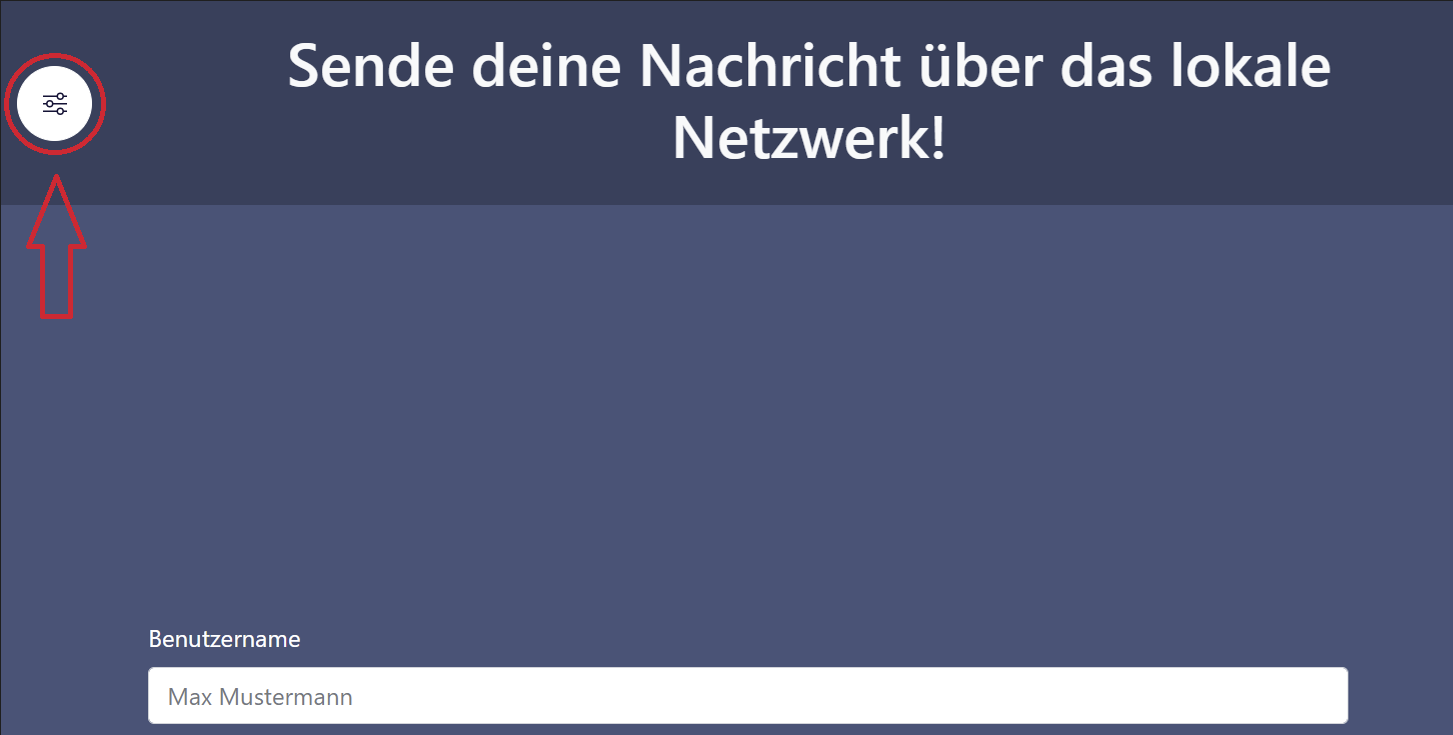
\includegraphics[width=\textwidth]{images/WebButton.png}
        \caption{Position des Buttons}
        \label{fig:webbut}
    \end{subfigure}
    \hfill
    \begin{subfigure}[b]{0.4\textwidth}
        \centering
        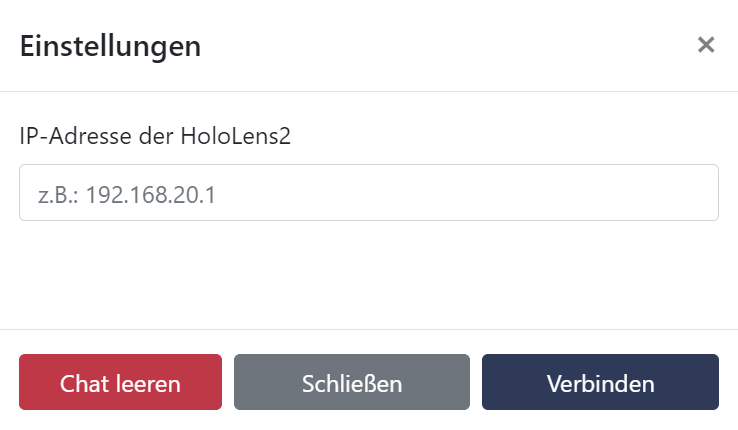
\includegraphics[width=\textwidth]{images/WebseiteSettings.png}
        \caption{Fenster der Webseite Einstellungen}
        \label{fig:websettings}
    \end{subfigure}
\end{figure}

Da die Webseite in einem Szenario mit zwei Geräten verwendet wird, muss eingestellt werden, auf welcher Seite des Kabels
sich das aktuelle Gerät befindet. Dies ist erforderlich, um die Nachrichten richtig in der virtuellen Umgebung zu simulieren. Dazu wählen Sie in der Combobox, siehe Abb. \ref{fig:websettings}, entweder \textit{Rechtes Gerät} oder \textit{Linkes Gerät}, abhängig von der Position des Trägers der Brille.

Nach der erfolgreichen Konfiguration der Webseite können nun Nachrichten versendet werden.

\subsubsection{\label{sec:cors}CORS}
CORS, oder Cross-Origin Resource Sharing, ist ein Sicherheitsmechanismus, der in modernen Webbrowsern implementiert ist. Seine Hauptaufgabe besteht darin, die Interaktionen zwischen verschiedenen Domains zu regulieren. In der Standardeinstellung erlauben Webbrowser aus Sicherheitsgründen nur Anfragen an Ressourcen, die sich auf derselben Domain befinden, von der die Anfrage stammt. Dies wird als Same-Origin-Policy bezeichnet.

CORS erweitert diese Grundfunktionalität, indem es den Zugriff auf Ressourcen von anderen Domains ermöglicht, vorausgesetzt, der Server, auf dem sich die Ressourcen befinden, erlaubt dies explizit. Dies ermöglicht eine sicherere und kontrolliertere Interaktion zwischen verschiedenen Domains. %TODO: QUELLEN

In unserem speziellen Fall, da unsere Kommunikation ausschließlich im lokalen Netzwerk stattfindet, ist es nicht unbedingt notwendig, strenge Sicherheitsmaßnahmen zu ergreifen. Dennoch ist es wichtig, dass wir bestimmte Header in allen Antworten einfügen, die von der Brille zurückgeschickt werden. Alle Anfragen werden im \textit{RequestManager.cs} Skript abgearbeitet. Genauere Infos sind im Abschnitt \ref{sec:webBackend} zu finden.

Diese Header welche einzubauen sind lauten:

\begin{lstlisting}[style=csharp label=code:CORS anfragen]
context.Response.Headers.Add("Access-Control-Allow-Origin", "*");
context.Response.Headers.Add("Access-Control-Allow-Methods", "GET, POST, OPTIONS");
context.Response.Headers.Add("Access-Control-Allow-Headers", "Content-Type");
\end{lstlisting}

\begin{itemize}
\item \textbf{``Access-Control-Allow-Origin``, "*"}: Dieser Header gibt an, von welchen Ursprüngen aus die Ressource zugänglich ist. Durch das Einstellen von "*" wird allen Ursprüngen erlaubt, auf die Ressource zuzugreifen, was als "Wildcard" für alle Ursprünge fungiert.
\item \textbf{``Access-Control-Allow-Methods``, "GET, POST, OPTIONS"}: Dieser Header gibt an, welche HTTP-Methoden für Cross-Origin-Anfragen erlaubt sind. Da wir nur GET, POST und OPTIONS-Anfragen an den Server senden, sind auch nur diese erlaubt, was bedeutet, dass Anfragen mit diesen Methoden von anderen Ursprüngen aus zugelassen werden.
\item \textbf{``Access-Control-Allow-Headers``, "Content-Type"}: Dieser Header gibt an, welche zusätzlichen Header in einer Anfrage aus einem anderen Ursprung erlaubt sind. In diesem Fall ist es nur der Header "Content-Type", was bedeutet, dass Anfragen von anderen Ursprüngen nur diesen spezifischen Header enthalten dürfen.
\end{itemize}

Durch das Hinzufügen dieser drei Zeilen zu unserer HTTP-Antwort fügen wir CORS-Header hinzu, die Cross-Origin-Anfragen für Ressourcen von unserem Server ermöglichen. Sie definieren auch genau, welche HTTP-Methoden und Header in diesen Anfragen erlaubt sind.

Falls beim Senden der Anfragen ein CORS-Fehler auftritt, liegt das vermutlich an der Konfiguration des Servers. Das Problem kann in Ausnahmefällen (zum Beispiel bei kleineren Testläufen) auf folgende Art und Weise umgangen werden:

\begin{itemize}
\item \textbf{Deaktivieren im Browser:} Die Deaktivierung von CORS im Browser würde das Problem beheben, birgt jedoch gewisse Risiken. CORS schützt den Benutzer vor schädlichen Webseiten, daher wird davon abgeraten. Die Deaktivierung erfolgt je nach Browser und ist nicht einfach zu finden. Stattdessen sollten die nachfolgende Lösung in Betracht gezogen werden.
\item \textbf{Verwendung von Plugins:} Es gibt Plugins, die CORS-Header von der Clientseite hinzufügen. Wir haben das Plugin \textit{moesif-origin-cors-change} getestet, das nur für den Chrome-Browser von Google verfügbar ist. Nach der Installation kann das Plugin bei Bedarf aktiviert/deaktiviert werden.
\end{itemize}

Es ist wichtig zu beachten, dass beide Lösungsvorschläge gewisse Sicherheitsrisiken bergen und nur im lokalen Netzwerk getestet wurden. Sie sind höchstens für erste Prototypen akzeptabel, wenn überhaupt. Nach der Verwendung unseres Programms sollten beide Konfigurationen wieder rückgängig gemacht werden.

\subsubsection{Bedienung der Webseite}
TODO: Bedienung und korrekte Simulation beschreiben.

% Keine Ahnung was Jonas hier macht aber ich füg mal mein Stuff ein hehe
\subsection{Frontend der Webseite} \marginpar{\small\(\rightarrow\) LAMPEL}
In diesem Abschnitt wird die Struktur und Entwicklung eines Frontends der Webseite zum Ping Anwendungsszenario erläutert. Besonderes Augenmerk wurde auf die zugrundeliegenden Entscheidungen bezüglich der Programmiersprachen sowie des Designprozesses gelegt.

Nach mehreren Entwicklungszyklen im ersten Anwendungsszenario wurde entschieden, eine Webseite in das Projekt zu integrieren. Die Funktionalität der Webseite sollte nahtlos in das Szenario integriert werden. Hierzu können Nachrichten und Absender direkt auf der Webseite eingetragen werden, um sie anschließend in die HoloLens-Applikation zu übertragen.

% https://www.webdesign-journal.de/website-konzept/
% https://textstrategin.de/2022/03/27/aufbau-einer-website-inhalte-und-struktur-richtig-planen-und-erstellen/
% https://link.springer.com/chapter/10.1007/978-3-658-02867-1_3
% https://de.ryte.com/magazine/10-tipps-website-konzept#Visuelles%20Website-Konzept
\subsubsection{Designprozess}
Beim Entwurf einer Webseite ist es essentiell, vor der eigentlichen Umsetzung die Farbpalette und das generelle Aussehen der Seite zu konzipieren. \footnote{Eins von den 4 idk \cite{.}} Da der Fokus auf der Anwendung auf der HoloLens liegt, wurde bewusst darauf geachtet, der Webseite nicht zu viel Aufmerksamkeit zu schenken. Sie sollte lediglich die grundlegenden Funktionen erfüllen, ohne dabei komplex zu sein. Aus diesem Grund ist die Webseite simpel gestaltet und verfügt über wenige Eingabefelder und wenig Text.

\subsubsection*{Webseitenprototyp}
Der Prototyp der Webseite, wie in Abbildung \ref{fig:protfrontend} dargestellt, gibt einen Überblick über das Frontend-Design. Das Zahnrad links oben öffnet ein Fenster, in dem die IP-Adresse der HoloLens eingegeben werden kann, um Nachrichten korrekt zu versenden. Auf der Hauptseite gibt es Eingabefelder für Benutzername und Nachricht. Der zeitlich sortierte Nachrichtenverlauf wird am rechten Rand angezeigt.

\begin{figure}[H]
\centering
\fbox{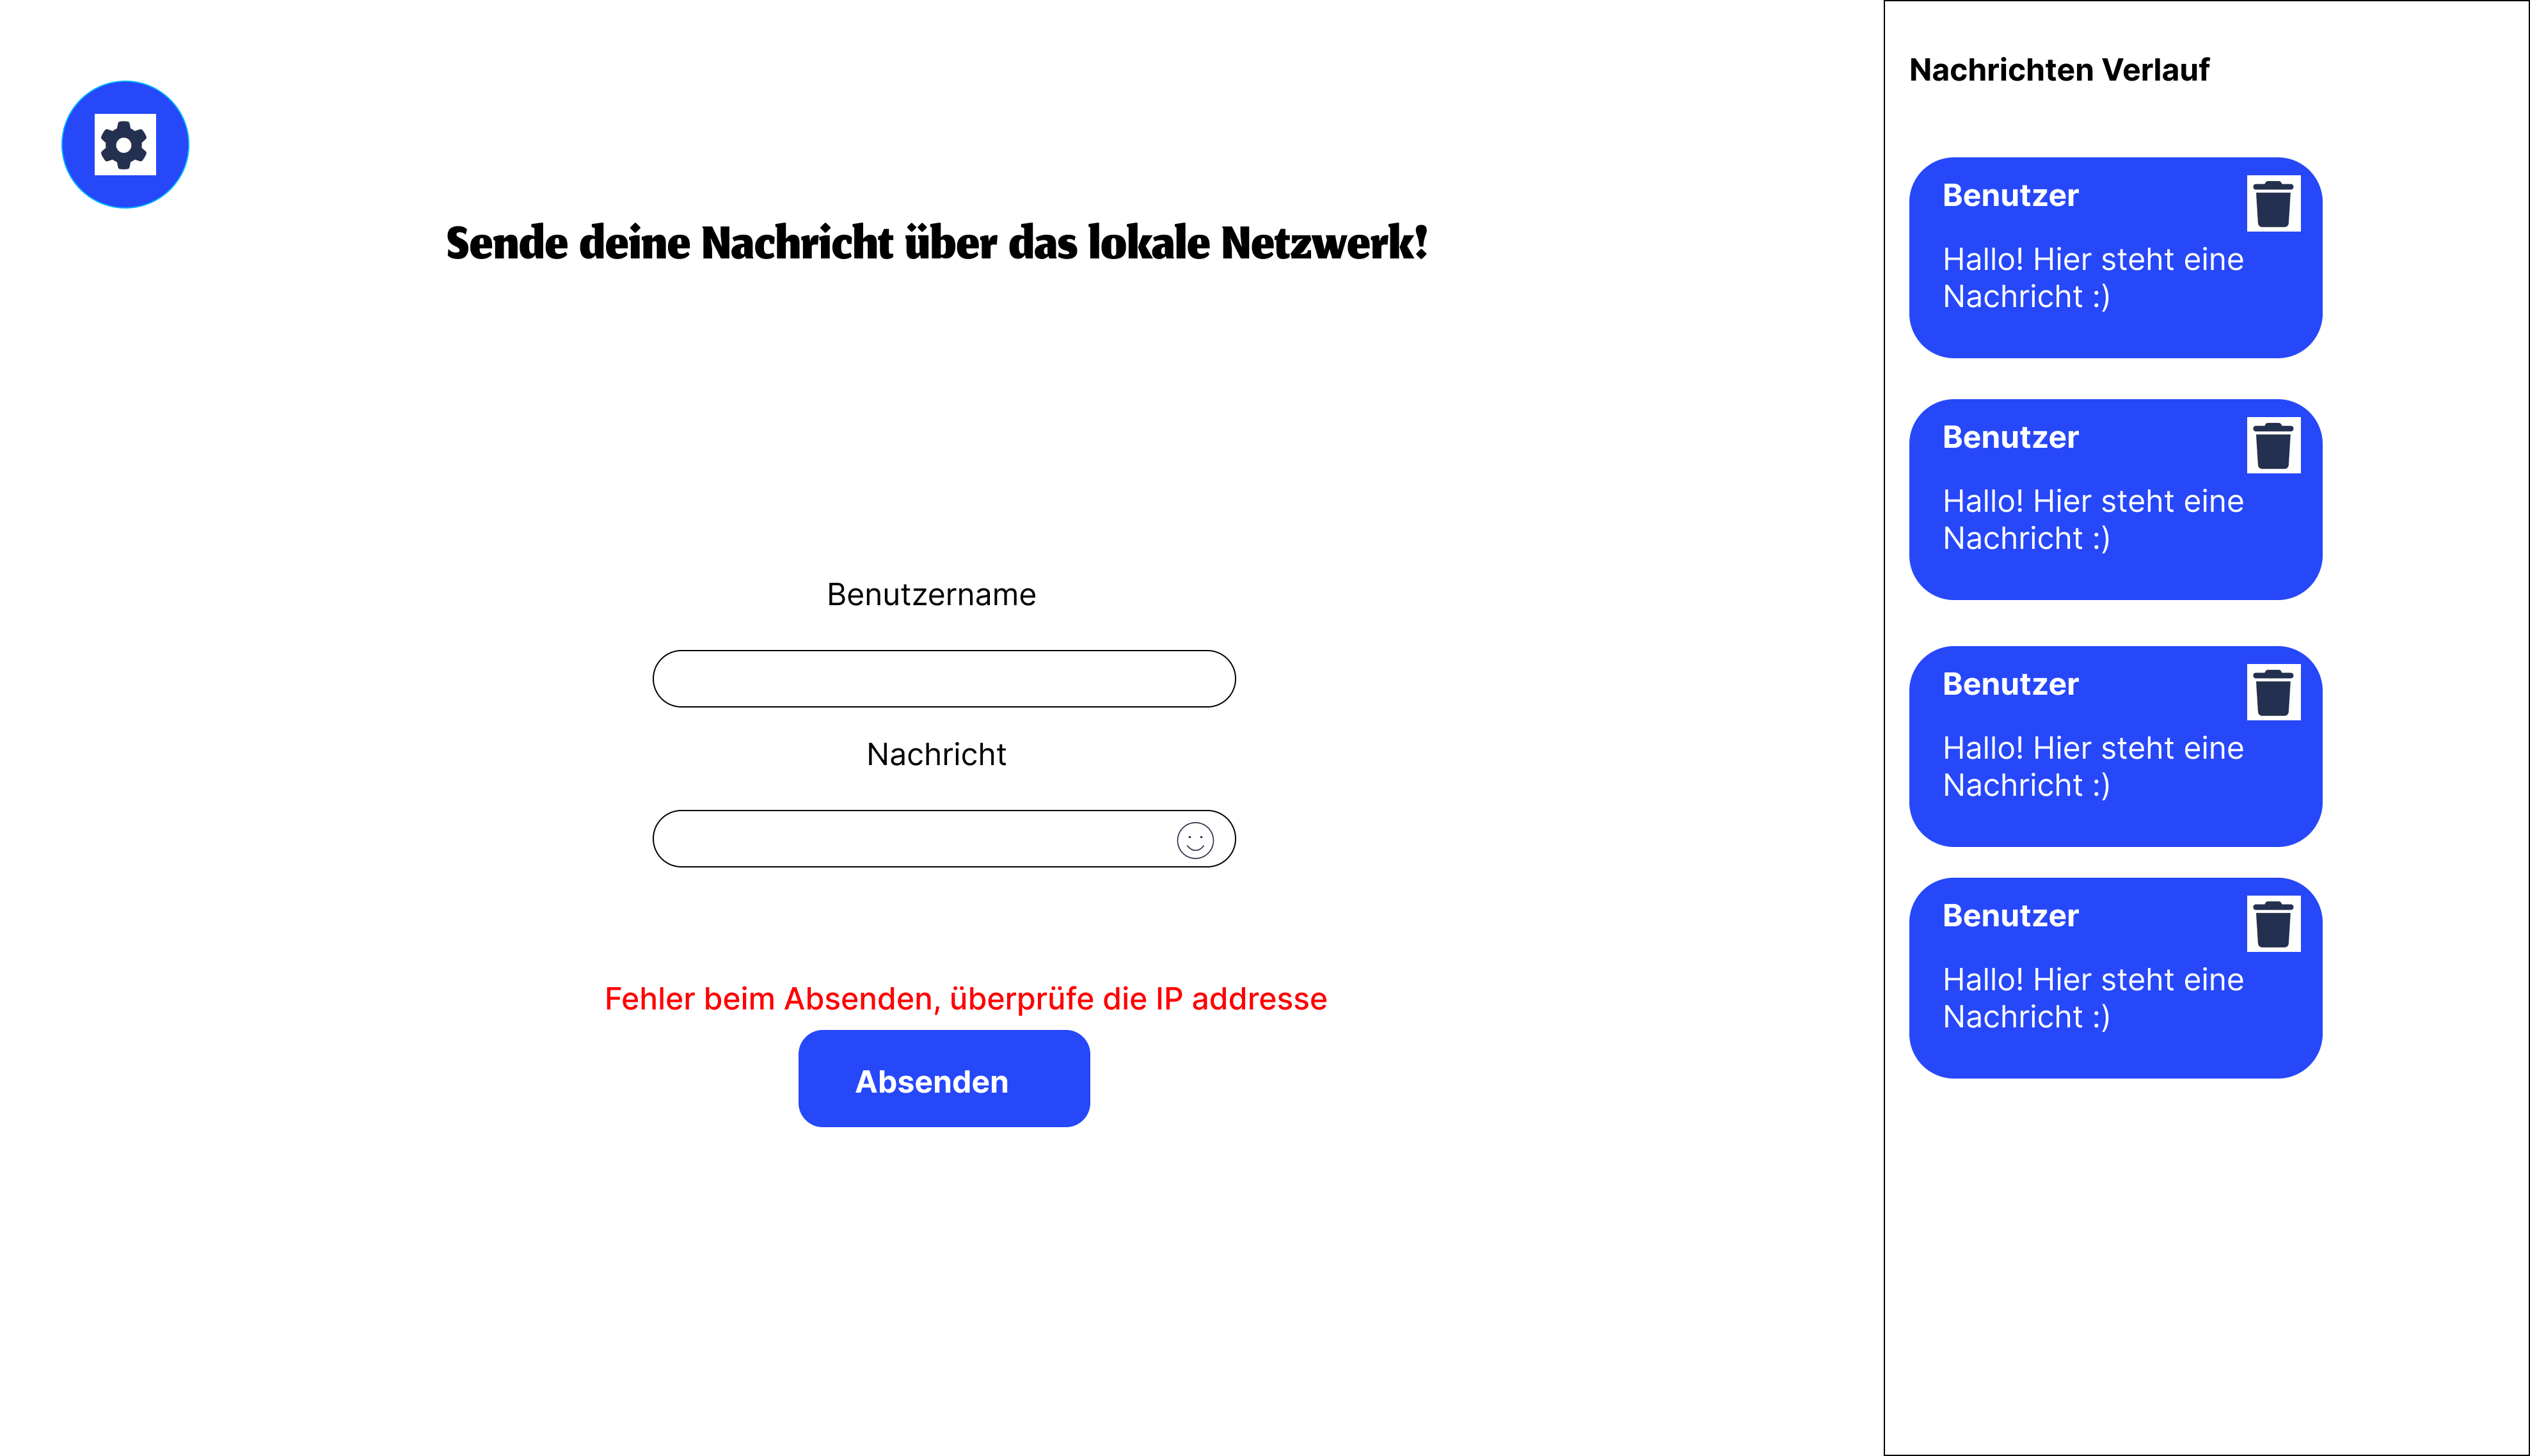
\includegraphics[width=1\textwidth]{images/prototypefrontend.png}}
\caption{Darstellung der Webseitenansicht aus Benutzersicht (Mockup)}
\label{fig:protfrontend}
\end{figure}

\subsubsection*{Ausprogrammierte Webseite}
Die endgültige Version der Webseite, wie in Abbildung \ref{fig:frontend} gezeigt, enthält alle gewünschten Funktionen. Die Farbpalette orientiert sich stark am Hauptmenü und den Standardfarben der HoloLens. Es werden verschiedene Blautöne verwendet, um eine konsistente und benutzerfreundliche Benutzererfahrung zu gewährleisten.

\begin{figure}[H]
\centering
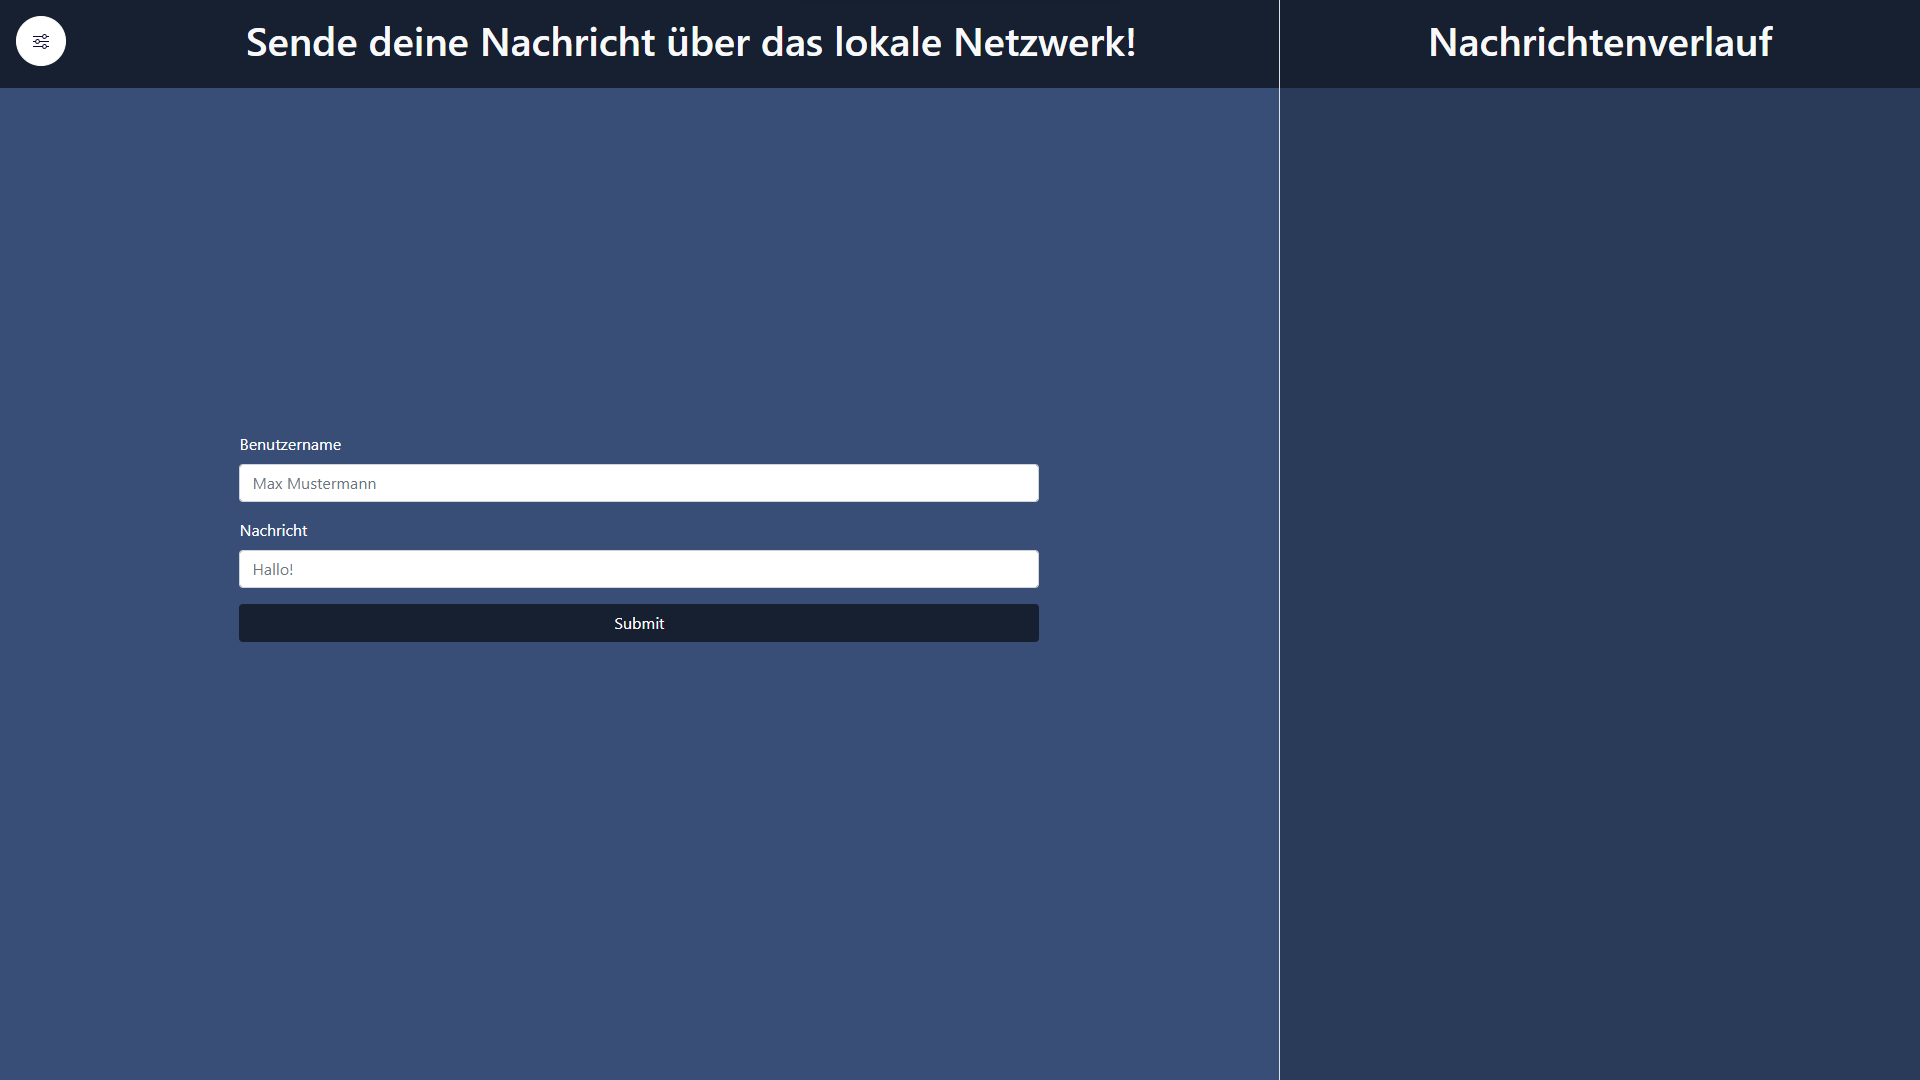
\includegraphics[width=1\textwidth]{images/frontend.png}
\caption{Darstellung der fertigen Webseitenansicht aus Benutzersicht}
\label{fig:frontend}
\end{figure}

Die Umsetzung des Designs hat zum Ziel, Verwirrungen zu vermeiden und eine nahtlose Integration der Webseite in das Gesamtsystem zu gewährleisten.

\subsubsection{Verwendete Programmiersprachen}
Für die Entwicklung der Webseite wurden hauptsächlich die Programmiersprachen \textit{HTML}, \textit{CSS} und \textit{JavaScript} verwendet. Zur Verbesserung des Designs und der Benutzererfahrung wurde außerdem das \textit{Framework Bootstrap} eingesetzt.

\subsubsection*{HTML (Hypertext Markup Language)}
HTML ist die grundlegende Struktursprache des World Wide Web. Es ermöglicht die Erstellung von Webseiten durch die Verwendung von Strukturelementen (Tags) für Überschriften, Absätze, Listen, Links und vieles mehr. Browser können HTML-Inhalte dem Standard entsprechend für den Anwender darstellen.
\footnote{Mozilla Developer Network \cite{HTML}}

\subsubsection*{CSS (Cascading Style Sheets)}
CSS ist eine Stylesheet-Sprache, die verwendet wird, um das Aussehen und die Formatierung von HTML-Dokumenten zu steuern. Es ermöglicht die Definition von Farben, Schriftarten, Layouts und anderen visuellen Eigenschaften einer Webseite. \footnote{Mozilla Developer Network \cite{CSS}}

CSS funktioniert durch das Zuweisen von Regeln und Stilen zu HTML-Elementen. Diese Regeln können in einer externen CSS-Datei definiert oder direkt im HTML-Dokument eingebettet werden.

\subsubsection*{JavaScript}
JavaScript ist eine dynamische Programmiersprache, die hauptsächlich für die clientseitige Entwicklung von Webanwendungen verwendet wird. Sie ermöglicht die Interaktion mit dem Benutzer, das Ändern von Inhalten in Echtzeit und die Steuerung des Verhaltens einer Webseite. \footnote{Mozilla Developer Network \cite{Javascript}}

JavaScript verbessert die Funktionalität einer Webseite, indem es auf Benutzerinteraktionen reagiert, Formulare validiert, Animationen erstellt und vieles mehr.

\subsubsection*{Integration von Bootstrap}
Bootstrap ist ein Open-Source-Framework für die Frontend-Entwicklung von Webseiten und Webanwendungen. Es bietet vorgefertigte HTML- und CSS-Vorlagen für Typografie, Formulare, Buttons, Navigation und andere UI-Komponenten. \footnote{Bootstrap Dokumentation \cite{Bootstrap}}

Bootstrap erleichtert die Erstellung responsiver und ästhetisch ansprechender Webseiten, indem es eine Reihe von vorgefertigten Designelementen und Layoutoptionen bereitstellt.

Die Integration von Bootstrap in eine HTML-Datei erfolgt durch das Einbinden der Bootstrap-Bibliotheksdateien in den \texttt{<head>}-Bereich des HTML-Dokuments. Dies kann entweder über ein CDN (Content Delivery Network) oder durch das Herunterladen und Einbinden der lokalen Bootstrap-Dateien erfolgen. \footnote{Bootstrap Dokumentation \cite{CDN-Links}}

Anschließend können Bootstrap-Komponenten und -Klassen innerhalb der HTML-Datei verwendet werden, um das Design und die Funktionalität der Webseite zu verbessern.

\subsubsection{Funktionen der Webseite}
Die Eingabefelder des Frontends brauchen Javascript Funktionen, um die gewünschten Tätigkeiten durchzuführen und so zu funktionieren wie eigentlich geplant.
\begin{lstlisting}[language=JavaScript, caption={Javascript | Ueberpruefung, ob die Eingabe eine Zahl oder . ist}]
function isNumberKey(evt) {
var charCode = (evt.which) ? evt.which : evt.keyCode;
if (charCode != 46 && charCode > 31 && (charCode < 48 || charCode > 57)) {
return false;
}
return true;
}
\end{lstlisting}
Die Funktion überprüft, ob die gedrückte Taste eine Zahlentaste ist. Sie wird auf der Webseite zur Überprüfung der Eingabe von der IP-Adresse genutzt, um sicherzustellen, dass nur Zahlen eingegeben werden können.

Die Funktion nimmt ein Event-Objekt als Parameter entgegen, das Informationen über das Tastaturereignis enthält. Der charCode wird aus dem Event-Objekt extrahiert, der den Unicode-Wert der gedrückten Taste darstellt. Die Funktion überprüft, ob die gedrückte Taste eine Zahl ist (der Unicode-Wert liegt im Bereich von 48 bis 57) oder der Punkt ist (der Unicode-Wert ist 46). Falls die gedrückte Taste im Bereich von 48 bis 57 liegt oder der Punkt ist, gibt die Funktion true zurück, was bedeutet, dass die Eingabe akzeptiert wird. Andernfalls gibt die Funktion false zurück, was bedeutet, dass die Eingabe nicht akzeptiert wird.

\begin{lstlisting}[language=JavaScript, caption={Javascript | Validierung und Senden der Message}, label=code:validatesend]
async function validateAndSendMessage() {
var username = document.getElementById("username").value.trim();
var message = document.getElementById("message").value.trim();

if (username !== '' && message !== '') {
const messageSent = await sendMessage(username, message);

if (!messageSent) {
alert("Message could not be sent.");
}
} else {
alert("Please fill in both fields!");
}
}
\end{lstlisting}
Die Funktion \texttt{validateAndSendMessage()} in dem Codeabschnitt \ref{code:validatesend} validiert die Eingaben in den Feldern für Benutzername und Nachricht und sendet die Nachricht nur ab, wenn beide Felder ausgefüllt sind.

Zunächst ruft die Funktion die Werte der Formularfelder für Benutzername und Nachricht ab und entfernt führende und abschließende Leerzeichen mit der trim()-Methode. Anschließend überprüft sie, ob sowohl der Benutzername als auch die Nachricht nicht leer sind. Wenn beide Felder nicht leer sind, wird die Funktion sendMessage(username, message) aufgerufen, um die Nachricht zu senden. Wenn die Nachricht erfolgreich gesendet wurde, wird nichts weiter unternommen. Andernfalls wird eine Warnmeldung angezeigt, dass die Nachricht nicht gesendet werden konnte. Sollte eines der Felder leer sein, wird dem Benutzer eine Warnmeldung angezeigt, die ihn darauf hinweist, beide Felder auszufüllen.

\subsection{Backend der Webseite} \marginpar{\small\(\rightarrow\) HAYLAZ}

Im vorherigen Abschnitt (\ref{sec:FrontendWebseite}) wurde der Designprozess der Webseite erläutert. Im Folgenden wird dieses Thema durch eine Beschreibung des Backend-Bereichs erweitert.

Die Webseite fungiert als Schnittstelle für die Kommunikation zwischen den beiden Laptops, die für das Szenario benötigt werden. Diese Kommunikation erfolgt über die Hololens, die gewissermaßen als "Mittelsmann" fungiert und die Datenübertragung ermöglicht.
\subsubsection{Protokoll zur Datenübertragung}

\begin{figure}[H]
    \centering
    \begin{minipage}[b]{0.45\textwidth}
        \centering
        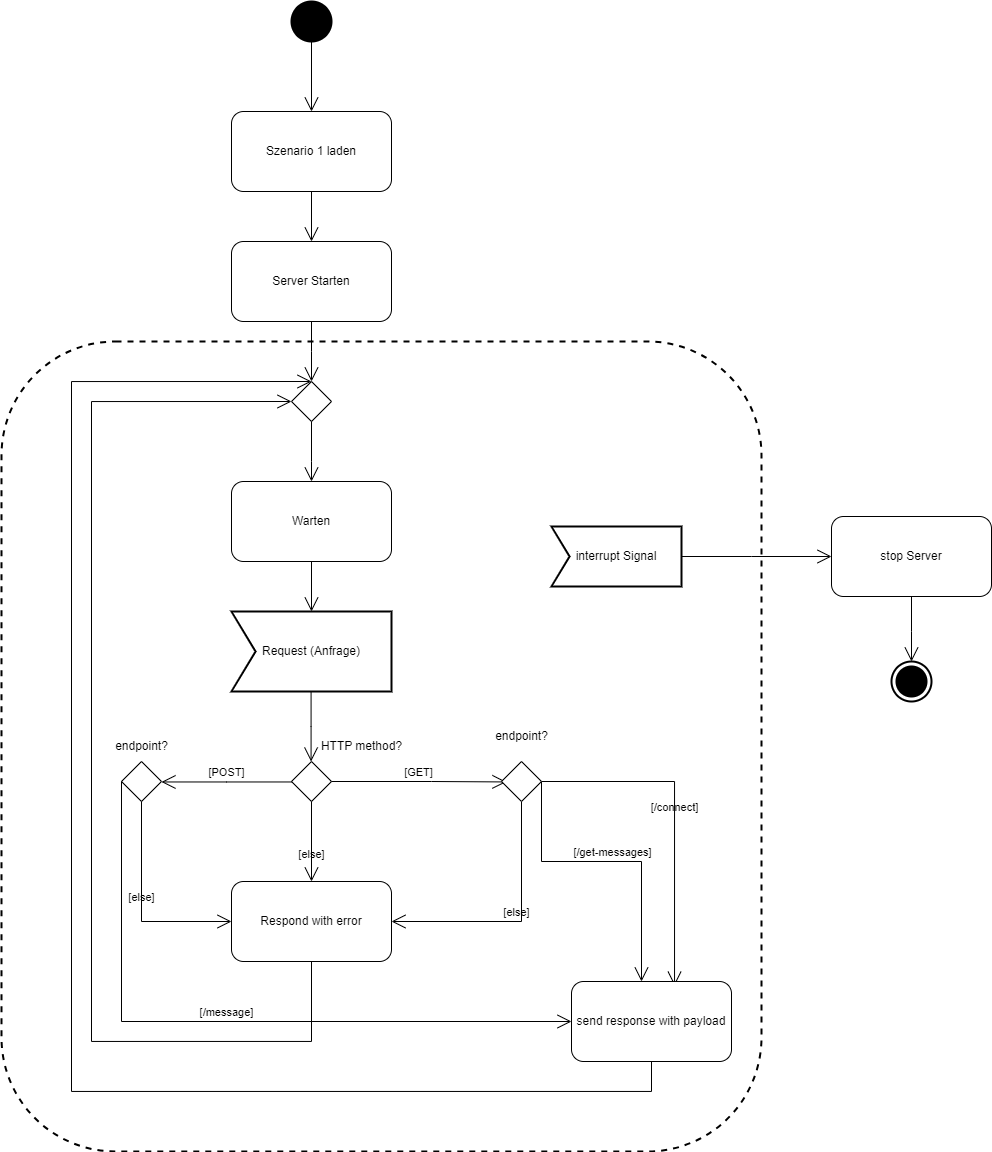
\includegraphics[scale=0.5]{images/serverStart.png}
        \caption{Aktivitätsdiagramm des Servers}
        \label{fig:protokoll}
    \end{minipage}
    \hfill
    \begin{minipage}[b]{0.45\textwidth}
        \centering
        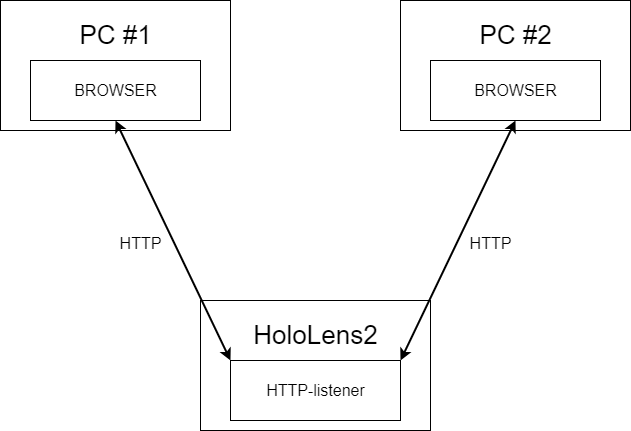
\includegraphics[scale=0.4]{images/laptopAufbau.png}
        \caption{Kommunikationsstruktur}
        \label{fig:struktur}
    \end{minipage}
\end{figure}

In Abbildung \ref{fig:protokoll} ist der Ablauf aller möglichen Szenarien dargestellt, wie eine solche Datenübertragung zustande kommen kann. Im Folgenden werden die einzelnen Schritte und ihre Funktionen beschrieben:

\begin{itemize}
\item \textbf{Start des Servers:} Auf der Hololens befindet sich ein Game-Objekt namens \textit{httpListener} mit einem Skript namens \textit{RequestManager.cs}. Beim Laden des ersten Szenarios wird ein HTTP-Listener in einem eigenen Thread gestartet. Erst wenn dieser läuft, kann auf Anfragen der Webseite reagiert werden. Eine ausführlichere Beschreibung der Funktionalität des Servers findet sich im Abschnitt \ref{sec:server}.
\item \textbf{Verbindungsaufbau:} Bevor ein Nachrichtenpaket gesendet werden kann, muss die IP-Adresse der Hololens registriert werden. Obwohl die Verbindungstestfunktion nicht zwingend erforderlich ist, um Nachrichten an diese IP zu senden, kann ein visuelles Feedback dem Benutzer anzeigen, ob die eingegebene IP-Adresse gültig ist und ob der Server erreichbar ist. Dies trägt zur Benutzerfreundlichkeit bei, indem es dem Benutzer ermöglicht, leichter zu erkennen, ob alles ordnungsgemäß funktioniert oder ob möglicherweise Probleme auftreten.
\item \textbf{Empfangen von Nachrichten:} Auf der Hololens wird eine Liste aktueller Nachrichten geführt. Beide Laptops rufen alle fünf Sekunden mit einem \textit{HTTP GET-Request} an den Endpunkt \textit{/get-messages} diese Liste ab. Dies ermöglicht eine kontinuierliche Aktualisierung des Nachrichtenverlaufs (\ref{sec:frontend}, \ref{fig:frontendImg}) und zeigt dem Benutzer stets die neuesten Nachrichten an.
\item \textbf{Versenden von Nachrichten:} Um eine Nachricht von einem Laptop auf den anderen zu senden, muss ein \textit{http post request} an den Endpoint \textit{/message} mit dem Benutzernamen und der Nachricht als Payload gesendet werden.
\end{itemize}

Es mag so aussehen, als ob das Senden von Requests für den Benutzer möglicherweise als unmöglich erscheint, aber im Abschnitt \ref{sec:Frontend} wird gezeigt, dass dies alles durch eine benutzerfreundliche Benutzeroberfläche (UI) erreicht wird.

Es ist festzuhalten, dass die beiden Laptops niemals direkt miteinander kommunizieren, sondern alle Nachrichten über den Server, die Hololens, laufen.

\subsubsection{\label{sec:server}Bearbeitung von Anfragen}
Die Bearbeitung von Anfragen erfolgt im Skript \textit{RequestManager.cs}. Der Listener wird in einem eigenen Thread
gestartet, da das Warten auf Nachrichten den Thread, auf dem der Listener läuft, blockiert. Nach dem Erhalt einer Anfrage
wird ein neues \textit{HttpListenerContext}-Objekt erstellt, und die Verarbeitung der Anfrage erfolgt in dem Thread, der
diesen Kontext bearbeitet. Wenn eine HTTP-Anfrage empfangen wird, ist der erste Schritt, zu überprüfen, um welche Art von
Anfrage es sich handelt. Ein POST und ein GET werden unterschiedlich verarbeitet. Bei Verwendung einer anderen HTTP-Methode
wird ein \textit{Method Not Allowed} Fehler zurückgesendet. Bei der Wahl des Endpunkts passiert dasselbe; jede nicht
unterstützte Anfrage auf einen Endpunkt wird mit einem \textit{Not Found} Fehler beantwortet.

Es werden in unserem Fall nur drei Endpunkte unterstützt:

\begin{itemize}
\item \textbf{Testen der Verbindung auf /connect}
\item \textbf{Empfangen von Nachrichten auf /get-messages}
\item \textbf{Senden einer Nachricht auf /message}
\end{itemize}

Um erfolgreich eine Anfrage an den Server zu senden, muss sie an die folgende Adresse
gehen: \texttt{http://{IP-Adresse der Hololens}:{Port}/{Endpoint}}. Die IP-Adresse der Hololens wird manuell auf der
Webseite eingegeben. Der Listener läuft standardmäßig auf dem Port 9090.

(Die erlaubten Endpunkte sind wie oben aufgeführt fallbasiert gelistet.)

\section{Knapsack Problem Szenario} \marginpar{\small\(\rightarrow\) SKREPEK}
Im zweiten Anwendungsszenario dieser Applikation liegt der Fokus auf dem bekannten Problem des Knapsack-Problems. Ziel
dieses Szenarios ist es, dieses Informatikproblem mithilfe von Augmented Reality (AR) visuell und spielerisch darzustellen.
Das Knapsack-Problem ist ein klassisches Problem der Informatik, das nicht nur an der Höheren Technischen Lehranstalt (HTL)
vermittelt wird, sondern auch von Schülern eigenständig programmiert werden soll. Dieser Ansatz dient dazu, den Anwendern
einen Einblick in die Informatik zu geben und möglicherweise Interessen für den Bereich zu wecken.

Das Unity-Anwendungsszenario für die HoloLens 2 bietet insgesamt eine interaktive und visuelle Erfahrung, bei der der
Benutzer nicht nur das Knapsack-Problem verstehen, sondern auch praktisch anwenden kann. Die Integration von AR ermöglicht
es dem Benutzer, das Problem in einer realen Umgebung zu erleben und die Optimierungsmöglichkeiten direkt zu visualisieren
und zu manipulieren. Diese immersive Herangehensweise kann dazu beitragen, das Verständnis des Knapsack-Problems zu vertiefen
und das Interesse an der Informatik zu fördern.

In diesem Abschnitt werden alle \textit{GameObjects}, \textit{Komponenten}, \textit{Scripts} und \textit{Klassen} genauer
erklärt, die in der Unity-Szene des Knapsack-Problems verwendet werden, um dieses zu realisieren.

\subsection{Knapsack-Problem Szenrio Hirarchie} \marginpar{\small\(\rightarrow\) SKREPEK}
Für einen sicheren und funktionalen Ablauf ist der Aufbau beziehungsweise die Hirarchie der Unity Szene von großer Bedeutung.
In diesem Abschnitt wird anhand der Abbildung \ref{fig:level2_hierarchy} verdeutlich wie die Unity Szene für die Implementierung
des zweiten Anwendungsszenarios für das Knapsack-Problem aufgebaut ist und es wird zusätzlich kurz darauf eingegangen
für was welches Objekt steht und welche Aufgabe dieses trägt.
\\
\begin{figure}[H]
    \centering
    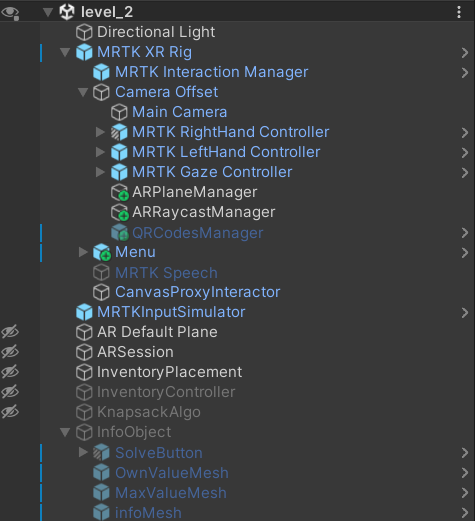
\includegraphics[scale=0.8]{images/Level2Hirarchy}
    \caption{Knapsack-Problem Szenario Hirarchie im Unity Editor.}
    \label{fig:level2_hierarchy}
\end{figure}
In dieser Abbildung ist die Hirarchie un der Inhalts des Knapsack-Problem Szenarios zu sehen. Anhand desen ist zu erkennen,
dass diese Unity Szene aus vielen wichtigen Komponenten besteht, die alle zusammenspielen, m das gewünschte Ergebnis
zu erzielen. Darunter sind folgende Objekte:
\begin{itemize}
    \item \textbf{level-2:} Ist die Unity Szene selbst, in der alle Game-Objekte enthalten sind.
    \item \textbf{MRTK XR Rig:} Grundbaustein für das Entwickeln einer XR-Applikation. Enthält wichtig Komponenten
    wie Controller für das tracken der Hände, für den User Gaze, etc.
    \item \textbf{UserInfo:} Text Objekt, dass in der \textit{main camera } liegt, damit dieses ständig im Sichtfeld des
    Benutzers liegt.
    \item \textbf{Managers:} Die drei Manager \textit{ARPlaneManager}, \textit{ARRaycastManager} und \textit{QRCodesManager}
    sind wichtiger Bestandteil um ARPlanes zu scannen, Raycasting durchzuführen und QRCodes zu erkennen.
    \item \textbf{HandMenu:} Knopf um in das Hauptmenu-Szenario zurück zu gelangen.
    \item \textbf{AR Default Plane:} Ist das Grund-Objekt für das markieren von erkannten ARPlanes.
    \item \textbf{ARSession:} Ist die Hauptkomponente, die die AR-Funktionalitäten steuert und koordiniert.
    \item \textbf{InventoryPlacementController:} Game Objekt, welches das platzieren des Inventar-Objekts handhabt.
    \item \textbf{InventoryController:} Game Objekt, welches das erkennen von neuen Objekten innerhalb des Inventar-Objekts handhabt.
    \item \textbf{KnapsackSolver:} Game Objekt, welches den Knapsack Algorithmus implementiert und das eigene Inventar berechnet.
    \item \textbf{bestSolutionPrefab:} Prefab, welches die perfekte Lösung wiederspiegelt.
    \item \textbf{InfoObject:} Dient der visualisierung von berechneten Werten und Fehlermeldungen.
\end{itemize}

In der Abbildung ist ausßredem zu sehen, dass ein Paar Game Objekte ausgegraut und nicht ausgegraut sind und, dass neben ein paar Game Objekten ein durchgestrichenes Auge zu sehen ist.
Wenn ein Game Objekt im Unity Editor ausgegraut ist bedeutet das, dass dieses GameObjekt und somit alle angehängiten Scripts von diesem Game Objekt deaktiviert sind.
Das bedeutet, dass dieses Game Objekt samt allen Scripts zu Szenenbeginn nicht aufgerufen und somit auch nicht ausgeführt werden. Nicht ausgegraute Game Objekte widerum sind
daher genau das Gegenteil. Das beudetet, dass das Game Objekt selbst samt allen angehängiten Scripts alle aktiviert sind und somit zu Szenenbeginn aufgerufen und ausgeführt werden.

Wenn neben einem Game Objekt das durchgestrichene Auge zu sehen ist bedeutet das nur, dass dieses Game Objekt im Unity Editor nicht zu sehen ist. Andererseits, wenn kein Zeichen
neben dem Game Objekt zu sehen ist, ist dieses Objekt im Unity Editor sichtbar. Dies dient dazu, dass falls in der Unity Szene viele Game Objekte vorhanden sind, dass man
diejenige ausblendet die nicht im Editor sichtbar sein müssen wie zum Beispiel Tesh Meshes oder Lables.

\subsection{Nutzung von QR-Codes} \marginpar{\small\(\rightarrow\) HAYLAZ}
Im vorherigen Abschnitt wurde bereits erwähnt, dass QR-Codes in diesem Level verwendet werden, um verschiedene Elemente zu repräsentieren. Diese QR-Codes spielen eine entscheidende Rolle, indem sie dazu dienen, vielfältige Informationen zu den einzelnen Gegenständen, die für das Knapsack-Inventar benötigt werden, zu speichern und sie anschließend in einer virtuellen Umgebung abzubilden. Im folgenden Abschnitt möchten wir näher darauf eingehen, wie genau diese QR-Codes generiert werden und welchen Zweck sie innerhalb der Augmented Reality (AR)-Applikation erfüllen. Dabei wird insbesondere betrachtet, wie die Codes generiert werden und auf welche Weise sie innerhalb der Anwendung zur Interaktion mit den realen Objekten verwendet werden.

\subsubsection{Struktur und Inhalt eines QR-Codes}
Die Informationen, die in einem QR-Code gespeichert werden können, sind begrenzt. In unserem Anwendungsfall wird lediglich
eine einzelne Zahl im Bereich von 1 bis 11 abgespeichert. Diese Zahlen repräsentieren die 11 verschiedenen Modelle, die
wir unterscheiden möchten. Da nur eine Zahl gespeichert wird, genügt ein QR-Code der Größe 21x21 Module (Version 1). Die
geringe Anzahl von Modulen ermöglicht eine schnellere Erkennung, auch über größere Distanzen.
%TODO: Quellen


TODO: Testen und Grafik erstellen um zu zeigen das es eine Rolle spielt welche version wir verwenden + wie groß die sind

Die zugehörigen Zahlen werden in der Software, genauer gesagt in der Klasse \textit{QRItem.cs}, mit Informationen verknüpft. Im folgenden Codeausschnitt wird dies verdeutlicht:

\begin{lstlisting}[style=csharp, caption={}, label=code:update]
public class QRItem
{
    public struct QRData
    {
        public int id;
        public string name;
        public Vector3 position;
        public int weight;
        public int value;
    }

    public QRData qrData;

    public Dictionary<int, QRData> items = new Dictionary<int, QRData>()
    {
        {1, new QRData { id = 1, name = "Laptop", weight = 70, value = 100 }},
        {2, new QRData { id = 2, name = "Router", weight = 25, value = 50 }},
        {3, new QRData { id = 3, name = "Maus", weight = 20, value = 30 }},
        // ...
        {11, new QRData { id = 11, name = "Handy", weight = 30, value = 100 }}
    };

    public QRItem(int id)
    {
        items.TryGetValue(id, out qrData);
    }
}
\end{lstlisting}

In dieser Klasse wird ein Dictionary verwendet, das den Gegenständen die folgenden Informationen zuordnet:

\begin{itemize}
    \item \textbf{Id:} Die numerische Kennung im QR-Code.
    \item \textbf{Name:} Die Bezeichnung des Gegenstandes, das dieser QR-Code repräsentiert.
    \item \textbf{Position:} Die Position des Gegenstandes in der virtuellen Umgebung.
    \item \textbf{Weight:} Das Gewicht des Gegenstandes.
    \item \textbf{Value:} Der Wert des Gegenstandes.
\end{itemize}

Diese Informationen spielen eine wesentliche Rolle in der weiteren Anwendung des Knapsack-Algorithmus.

\subsubsection{QR-Code-Tracking}
Das Tracking der QR-Codes erfolgt mithilfe des \textit{QRCodeManager.cs} Skripts. Dieses Klasse ist ein Singleton, das
die Erkennung und Verfolgung der QR-Codes steuert.
%TODO: Quelle: Singelton

Nach der Erkennung eines QR-Codes erfolgen eine Reihe von Schritten, um diese Informationen zu speichern, verarbeiten
und zuletzt darzustellen.
Hier eine kurze Übersicht:

\begin{figure}[H]
\centering
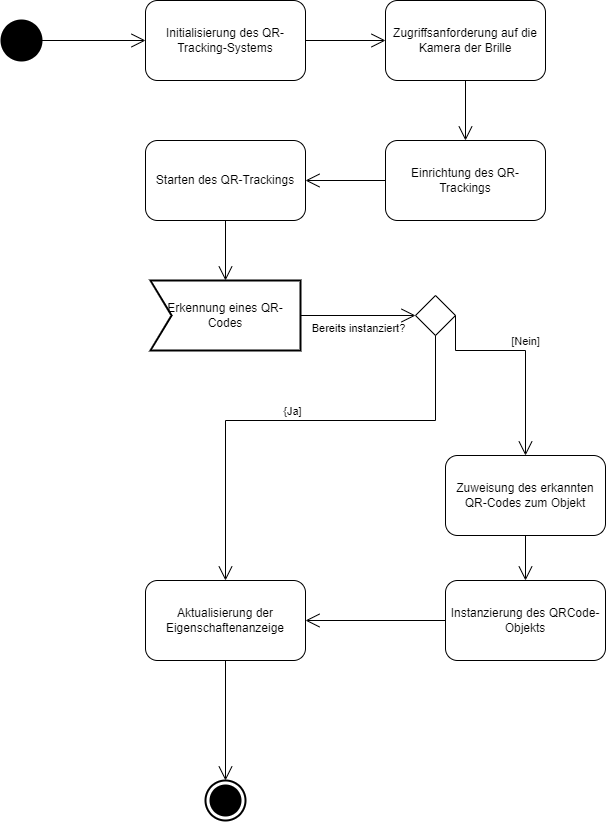
\includegraphics[scale=0.5, angle=0]{images/QRAblauf}
\caption{Ablaufdiagramm des QR-Code-Trackings.}
\label{fig:qrtracking}
\end{figure}

\begin{itemize}

\item \textbf{Initialisierung des QR-Tracking-Systems:}
Um das QR-Tracking-System zu aktivieren, wird die erforderliche Komponente gestartet, um die Erkennung von QR-Codes zu ermöglichen. Diese Komponente ist das QRCodeManager-Game-Objekt, das weitere Game-Objekte instanziiert, wie beispielsweise den \textit{QRCodesVisualizer}, der für die Visualisierung benötigt wird (siehe Abschnitt \ref{sec:qrvisualizer}). Dabei werden Tracking-Algorithmen gestartet, die für die Lokalisierung und Identifizierung von QR-Codes in der Umgebung benötigt werden. Diese Initialisierung erfolgt zu Beginn der Anwendungsaktivität.

\item \textbf{Zugriffsanforderung auf die Kamera der Brille:}
%TODO: Hier ein Bild von "Camera acess needed" einfügen
Für das QR-Tracking wird der Zugriff auf die Kamera der Augmented-Reality-Brille benötigt. Eine Zugriffsanfrage wird
gestellt, um die notwendigen Berechtigungen zu erhalten. Dieser Schritt ist entscheidend, um visuelle Daten von der Kamera
zu erhalten und QR-Codes in der physischen Umgebung zu erkennen.

\item \textbf{Einrichtung des QR-Trackings:}
Die Einrichtung des QR-Trackings umfasst die Konfiguration von Parametern und Einstellungen, die für die korrekte
Funktion des Tracking-Systems erforderlich sind.Dazu gehören Kalibrierungsschritte, die Anpassung an die Umgebung und die
Festlegung von Erkennungsbereichen. Eine ordnungsgemäße Einrichtung gewährleistet eine zuverlässige und präzise Erkennung von QR-Codes.

\item \textbf{Starten des QR-Trackings:}
Das System sucht aktiv nach QR-Codes in der Umgebung, um sie zu erkennen. Die Kamera erfasst kontinuierlich visuelle
Daten, welche von den Tracking-Algorithmen analysiert werden, um QR-Codes zu identifizieren. Das Starten des Trackings
markiert den Beginn des fortlaufenden Erkennungsprozesses.

\item \textbf{Erkennung eines QR-Codes (Event):}
Sobald die Kamera einen QR-Code erfasst, wird dieser automatisch erkannt. Dieses Ereignis signalisiert die erfolgreiche Erkennung eines QR-Codes und liefert Informationen über den erkannten QR-Code, wie seine Daten und Position. Eine detaillierte Beschreibung des genauen Ablaufs der Erkennung und Positionsbestimmung ist im Abschnitt \ref{sec:QRPositionsbestimmung} zu finden.

\item \textbf{Zuweisung des erkannten QR-Codes zum Objekt:}
Nach der Erkennung wird überprüft, ob der erkannte QR-Code bereits in der Anwendung registriert ist. Falls dies der Fall
ist, wird der erkannte QR-Code einem entsprechenden Objekt in der virtuellen Umgebung zugeordnet.

\item \textbf{Instanzierung des QRCode-Objekts:}
Nach dem Scannen eines QR-Codes wird ein QR-Code-Prefab erzeugt und in der Szene platziert.

Dieses Objekt dient als Repräsentation des gescannten QR-Codes und wird als QR-Objekt bezeichnet. Es enthält visuelle
Darstellungen, Interaktionsmöglichkeiten und weitere relevante Informationen über den zugehörigen QR-Code. Die Instanziierung
ermöglicht eine nahtlose Integration des gescannten QR-Codes in die virtuelle Umgebung. Weitere Informationen zur Visualisierung
von QR-Codes finden Sie in Abschnitt \ref{sec:qr_visualization}.

\item \textbf{Aktualisierung der Eigenschaftenanzeige:}
Die Aktualisierung der Eigenschaftsanzeige dient dazu, visuelle und informative Darstellungen des erkannten QR-Codes zu
aktualisieren. Hierbei werden die Position, Größe, visuelle Darstellung und zugehörige Informationen des QR-Codes aktualisiert.
Durch die Aktualisierung wird sichergestellt, dass die Benutzer stets die neuesten Informationen über das durch den QR-Code
repräsentierte Objekt erhalten.

\end{itemize}

\subsubsection{Interaktion mit QR-Codes}
\begin{figure}[H]
\centering
\includegraphics[scale=0.04, angle=0]{images/bauklotz}
\caption{Bauklötze mit QR-Codes}
\label{fig:bauklotz}
\end{figure}

Durch die Verwendung der HoloLens können wir dem Benutzer eine visuelle Darstellung einer virtuellen Welt bieten. Um eine
Verbindung zwischen der realen und der virtuellen Welt herzustellen, nutzen wir QR-Codes.  Diese dienen in der realen Welt als Repräsentationen jener Objekte, die wir in der virtuellen Welt darstellen möchten.

Wie in \ref{fig:bauklotz} zu sehen ist, sind die Bauklötze mit QR-Codes versehen. Diese Bauklötze repräsentieren die Gegenstände,
die der Benutzer in sein Inventar aufnehmen kann. Wenn der Benutzer einen Bauklotz aufhebt und ihn der HoloLens nähert, wird
der QR-Code gescannt. Dadurch werden Informationen wie das zugehörige 3D-Modell, der Wert, das Gewicht und der Name des
Gegenstands angezeigt. Auf diese Weise können wir eine nahtlose Verbindung zwischen der realen und der virtuellen Welt
herstellen.

Dem Benutzer wird die Möglichkeit geboten, die Bauklötze physisch zu berühren, aufzuheben und zu fühlen. Diese sensorische
Erfahrung trägt dazu bei, die Immersion des Benutzers zu verbessern und ihm ein besseres Verständnis der virtuellen Welt
zu ermöglichen. Dazu muss laufend die Position der Bauklötze und somit auch der QR-Codes getrackt werden, wie im Abschnitt
\ref{sec:qrpos} beschrieben.



\subsubsection{\label{sec:qrpos}Positionsbestimmung von QR-Codes}
Um die räumliche Position eines QR-Codes exakt zu bestimmen, ist ein spezieller Prozess notwendig. Dieser Schritt ist entscheidend, um physische QR-Codes in der virtuellen Realität darstellen und mit ihnen interagieren zu können. Die Positionierung der QR-Codes erfolgt mit Hilfe einer Klasse namens \textit{QRWatcher}, die im SDK-Plugin \textit{Microsoft.MixedReality.QR} enthalten ist.

Die \textit{QRWatcher}-Klasse ermöglicht die Erkennung und Verfolgung von QR-Codes in der physischen Umgebung. Sie stellt eine Vielzahl von Funktionen und Ereignissen zur Verfügung, die für die Weiterverarbeitung von QR-Codes notwendig sind. Die Verarbeitung erfolgt in den folgenden Schritten:

\begin{itemize}
\item \textbf{Kamera-Feed abrufen:} Nach der Initialisierung der \textit{QRWatcher}-Klasse und dem Start des Trackings wird zunächst der Kamerafeed der HoloLens abgerufen.
\item \textbf{Bildverarbeitung:} Der Kamerafeed wird mit den Algorithmen und Methoden der \textit{QRWatcher}-Klasse verarbeitet, um QR-Codes zu identifizieren.
\item \textbf{Erkennung eines QR-Codes:} Sobald ein QR-Code erkannt wird, wird ein Ereignis ausgelöst. Dieses Ereignis enthält Informationen über den erkannten QR-Code, wie dessen Daten und Position, und kann von anderen Klassen subskribiert werden.
\item \textbf{Übersetzung der Positionen:} Die Positionen der erkannten QR-Codes werden in die Weltkoordinaten der HoloLens übersetzt, um sie in der virtuellen Welt zu verankern. Dazu wird ein \textit{Spatial Graph Node}(\ref{sec:SGN}) erstellt und die Position des QR-Codes an diesen gebunden.
\textbf{Zuordnung des QR-Codes:} Nach der Erkennung wird überprüft, ob der erkannte QR-Code bereits in der Anwendung registriert ist. Falls ja, werden die Positionsinformationen des QR-Codes aktualisiert, um mögliche Bewegungen in der physischen Umgebung zu berücksichtigen. Anschließend wird ein neuer \textit{Spatial Graph Node} an dieser aktualisierten Position platziert. Dadurch wird sichergestellt, dass das virtuelle Objekt weiterhin korrekt mit dem QR-Code verbunden ist und an der aktuellen Position in der virtuellen Umgebung angezeigt wird.
\end{itemize}

Nach Abschluss dieser Schritte sind die Positionen der vorhandenen QR-Codes bestimmt und können im nächsten Schritt in der virtuellen Welt dargestellt werden.

\subsubsection{Visualisierung von QR-Codes}
Nachdem die genaue Platzierung der QR-Codes bestimmt wurde, muss ihre Visualisierung in der virtuellen Welt umgesetzt werden. Hierfür nutzen wir die Funktionalität von Unity Prefabs, die die Erstellung visueller Repräsentationen der QR-Codes und ihre nahtlose Integration in die virtuelle Umgebung ermöglichen.

Die Klasse \textit{QRWatcher} kann drei Events auslösen: das Erkennen eines neuen QR-Codes, das Erkennen eines bereits bekannten QR-Codes und das Löschen eines QR-Codes.

Die \textit{Visualizer}-Klasse reagiert auf alle diese Events. Beim erstmaligen Erkennen eines QR-Codes wird ein QR-Prefab initialisiert. Bei erneutem Erkennen werden die Positionsdaten aktualisiert, und beim Entfernen wird entsprechend der QR-Code-Prefab aus der Szene entfernt.

Jedes Prefab enthält alle relevanten Informationen für die Darstellung des QR-Codes, einschließlich des 3D-Modells, des Namens, des Werts und anderer Daten, die für Interaktionen innerhalb der virtuellen Umgebung erforderlich sind. Um die Funktionalität des QR-Codes sicherzustellen, wird dem Prefab das Skript \textit{QRCodes.cs} zugewiesen, das die visuelle Darstellung und alle damit verbundenen Interaktionen steuert.

\begin{figure}[H]
\centering
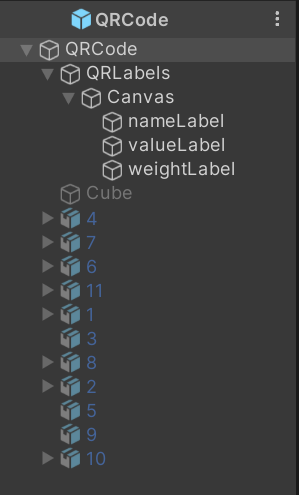
\includegraphics[scale=0.04, angle=0]{images/qrprefab}
\caption{Hierarchie des QR-Code Prefabs}
\label{fig:qrprefab}
\end{figure}


In diesem Abschnitt werden die Eigenschaften eines einzelnen QR-Codes erläutert. Wie zu erkennen ist, verfügt dieses Prefab über nur wenige Eigenschaften, nämlich:
\begin{itemize}
\item \textbf{Canvas:} Der Canvas enthält drei Labels: "Name", ``Gewicht`` und "Wert", welche die für den Benutzer relevanten Eigenschaften eines Gegenstandes anzeigen.
\item \textbf{GameObjects von 1 bis 11:} Diese GameObjects repräsentieren die 3D-Modelle, die der QR-Code darstellen soll. Weitere Details zu den 3D-Modellen sind im Abschnitt \ref{sec:3dModelleDustin} zu finden. Jedes Prefab enthält die Modelle aller möglichen Items, die angezeigt werden können. Die Nummerierung erleichtert die Iteration durch diese Modelle in der Szene, da die QR-Codes eine eindeutige ID haben und mit einem numerischen Namen leichter darauf zugegriffen werden kann.
\end{itemize}

\begin{lstlisting}[style=csharp, caption={Instanzierung eines QR-Prefabs}, label=code:QR-Prefab instanzierung]
void Start()
{
    //... weiterer Code

    // Die physikalische Größe des QR-Codes wird abgerufen; Wird für Berechnungen in der UpdatePropertiesDisplay() Funktion benötigt
    PhysicalSize = qrCode.PhysicalSideLength;

    try
    {
        // (1) Ein neues QRItem wird erstellt und mit den Daten des gescannten QR-Codes initialisiert
        item = new QRItem(int.Parse(qrCode.Data));

        // (2) Das entsprechende 3D-Modell wird anhand der ID des QR-Items gefunden
        model = gameObject.transform.Find(item.qrData.id.ToString()).gameObject;

        // (2) Falls ein 3d-Modell gefunden wurde wird sie in der AR-Umgebung sichtbar gesetzt
        model.SetActive(model != null);
    }
    catch (System.Exception e)
    {
        // Fehlerbehandlung, falls das Parsing der QR-Code-Daten fehlschlägt
        Debug.LogError("Error parsing QR Code data: " + e.Message);
    }

    // (3)Labels werden mit den entsprechenden Werten befüllt
    setLabels();
}
\end{lstlisting}

Nach der Instanzierung eines QR-Prefabs wird der folgende Codeabschnitt (\ref{code:QR-Prefab instanzierung}) ausgeführt. Das Skript \textit{QRCode.cs}, in dem sich dieser Abschnitt befindet, erhält bei der Instanzierung lediglich den Inhalt des gescannten QR-Codes übermittelt, nämlich die ID. \textit{(1)} Anhand dieser ID werden aus einer Liste möglicher Objekte die weiteren erforderlichen Informationen entnommen und innerhalb der Klasse gespeichert. \textit{(2)} Zudem wird das entsprechende 3D-Modell in die Szene eingefügt. \textit{(3)} Zuletzt werden die Labels mit den richtigen Werten (Name, Gewicht, Wert) befüllt, \ref{code:labels} ist der genauere Codeabschnitt. Diese Aktionen werden bei jeder Instanzierung nur einmal ausgeführt. Im Gegensatz dazu wird die folgende Funktion (\ref{code:Aktualisieren der Position}) bei jeder Frame aktuallisierung der Brille ausgeführt und befindet sich daher in der \textit{Update()} Funktion. Weitere Informationen zu den Lebeszyklusmethoden befinden sich in diesem abschnitt: \ref{sec:Shrek is leben}

\begin{lstlisting}[style=csharp, caption={Setzen der Labels}, label=code:labels]
private void setLabels()
{
    //Das GameObject mit den Labels wird gespeichert
    labels = gameObject.transform.Find("QRLabels").gameObject;

    try
    {
        //Der Canvas indem sich die Labels befinden wird gespeichert
        Transform canvas = labels.transform.Find("Canvas");

        //Die Text-Komponenten indem sich der anzuzeigende Text befindet wird geseichert
        TextMeshProUGUI nameLabel = canvas.Find("nameLabel").gameObject.GetComponent<TextMeshProUGUI>();
        TextMeshProUGUI valueLabel = canvas.Find("valueLabel").gameObject.GetComponent<TextMeshProUGUI>();
        TextMeshProUGUI weightLabel = canvas.Find("weightLabel").gameObject.GetComponent<TextMeshProUGUI>();

        // Die Texte der Labels werden mit den entsprechenden Daten des QR-Items aktualisiert
        nameLabel.text = "Name: " + item.qrData.name;
        valueLabel.text = "Wert: " + item.qrData.value.ToString();
        weightLabel.text = "Gewicht: " + item.qrData.weight.ToString();

        // Die Farben der Labels werden gesetzt
        nameLabel.color = Color.white;
        valueLabel.color = Color.yellow;
        weightLabel.color = Color.cyan;

    }
    catch (System.Exception e)
    {
        // Fehlerbehandlung, falls beim abfragen der Modelle etwas schiefläuft
        Debug.LogError("Error setting labels: " + e.Message);
    }
}
\end{lstlisting}

Dieser Code ist dafür verantwortlich, die Textlabels im Canvas entsprechend mit den Daten des gescannten QR-Codes zu aktualisieren. Zuerst wird das GameObject "QRLabels" gefunden, das die Labels enthält. Dann werden die Textkomponenten innerhalb des Canvas-GameObjects gesucht und mit den entsprechenden Daten aktualisiert. Dieser Prozess wird jedes Mal durchgeführt, wenn ein neuer QR-Code gescannt und instanziiert wird.


\begin{lstlisting}[style=csharp, caption={Aktualisieren der Position}, label=code:Aktualisieren der Position]
void UpdatePropertiesDisplay()
{
    if (qrCode != null && lastTimeStamp != qrCode.SystemRelativeLastDetectedTime.Ticks)
    {
        PhysicalSize = qrCode.PhysicalSideLength;

        item.qrData.position = new Vector3(PhysicalSize / 2.0f, PhysicalSize / 2.0f, 0.0f);

        labels.transform.localPosition = new Vector3(item.qrData.position.x + 0.05f, item.qrData.position.y, item.qrData.position.z);

        labels.transform.localScale = new Vector3(PhysicalSize * 0.02f, PhysicalSize * 0.02f, 0.005f);

        model.transform.localPosition = item.qrData.position;

        lastTimeStamp = qrCode.SystemRelativeLastDetectedTime.Ticks;
    }
}
\end{lstlisting}
Die Funktionsweise der Positionsbestimmung ist im Abschnitt (\ref{sec:qrpos}) beschrieben. Im Codeabschnitt \ref{code:Aktualisieren der Position} werden die bereitgestellten Positionsdaten verwendet, um die Position der Modelle zu aktualisieren. Hier ist eine schrittweise Erläuterung dessen, was innerhalb der Funktion passiert:
\begin{itemize}
\item Zunächst wird überprüft, ob der QR-Code nicht null ist und ob sich die Zeitmarke des letzten erkannten QR-Codes seit dem letzten Mal geändert hat. Diese Überprüfung stellt sicher, dass die Aktualisierung der Anzeige nur erfolgt, wenn sich tatsächlich etwas geändert hat, was zur Effizienz und Leistung der Anwendung beiträgt.
\item Die Position des QR-Codes (\textit{item.qrData.position}) wird so festgelegt, dass er sich in seinem lokalen Koordinatensystem zentriert. Dazu wird die Position auf \textit{(PhysicalSize / 2.0f, PhysicalSize / 2.0f, 0.0f)} gesetzt, wobei \textit{PhysicalSize} die Größe des QR-Codes ist. Diese Festlegung ermöglicht es, dass der QR-Code unabhängig von seiner Größe korrekt positioniert wird.
\item Die Position der labels wird relativ zur Position des QR-Codes eingestellt, mit einem Offset von 0.05f nach rechts, aber auf derselben Höhe (y-Koordinate) und Tiefe (z-Koordinate). Die Skalierung der labels wird auf \textit{(PhysicalSize * 0.02f, PhysicalSize * 0.02f, 0.005f)} gesetzt. Dies bedeutet, dass die Größe der Labels entsprechend der Größe des QR-Codes angepasst wird.
\item Die Position des 3D-Modells, das mit dem QR-Code verbunden ist wird auf die Position des QR-Codes gesetzt. Schließlich wird \textit{lastTimeStamp} auf die aktuelle Zeitmarke des QR-Codes gesetzt, um festzuhalten, wann der QR-Code zuletzt erkannt wurde.

\end{itemize}

\begin{figure}[H]
\centering
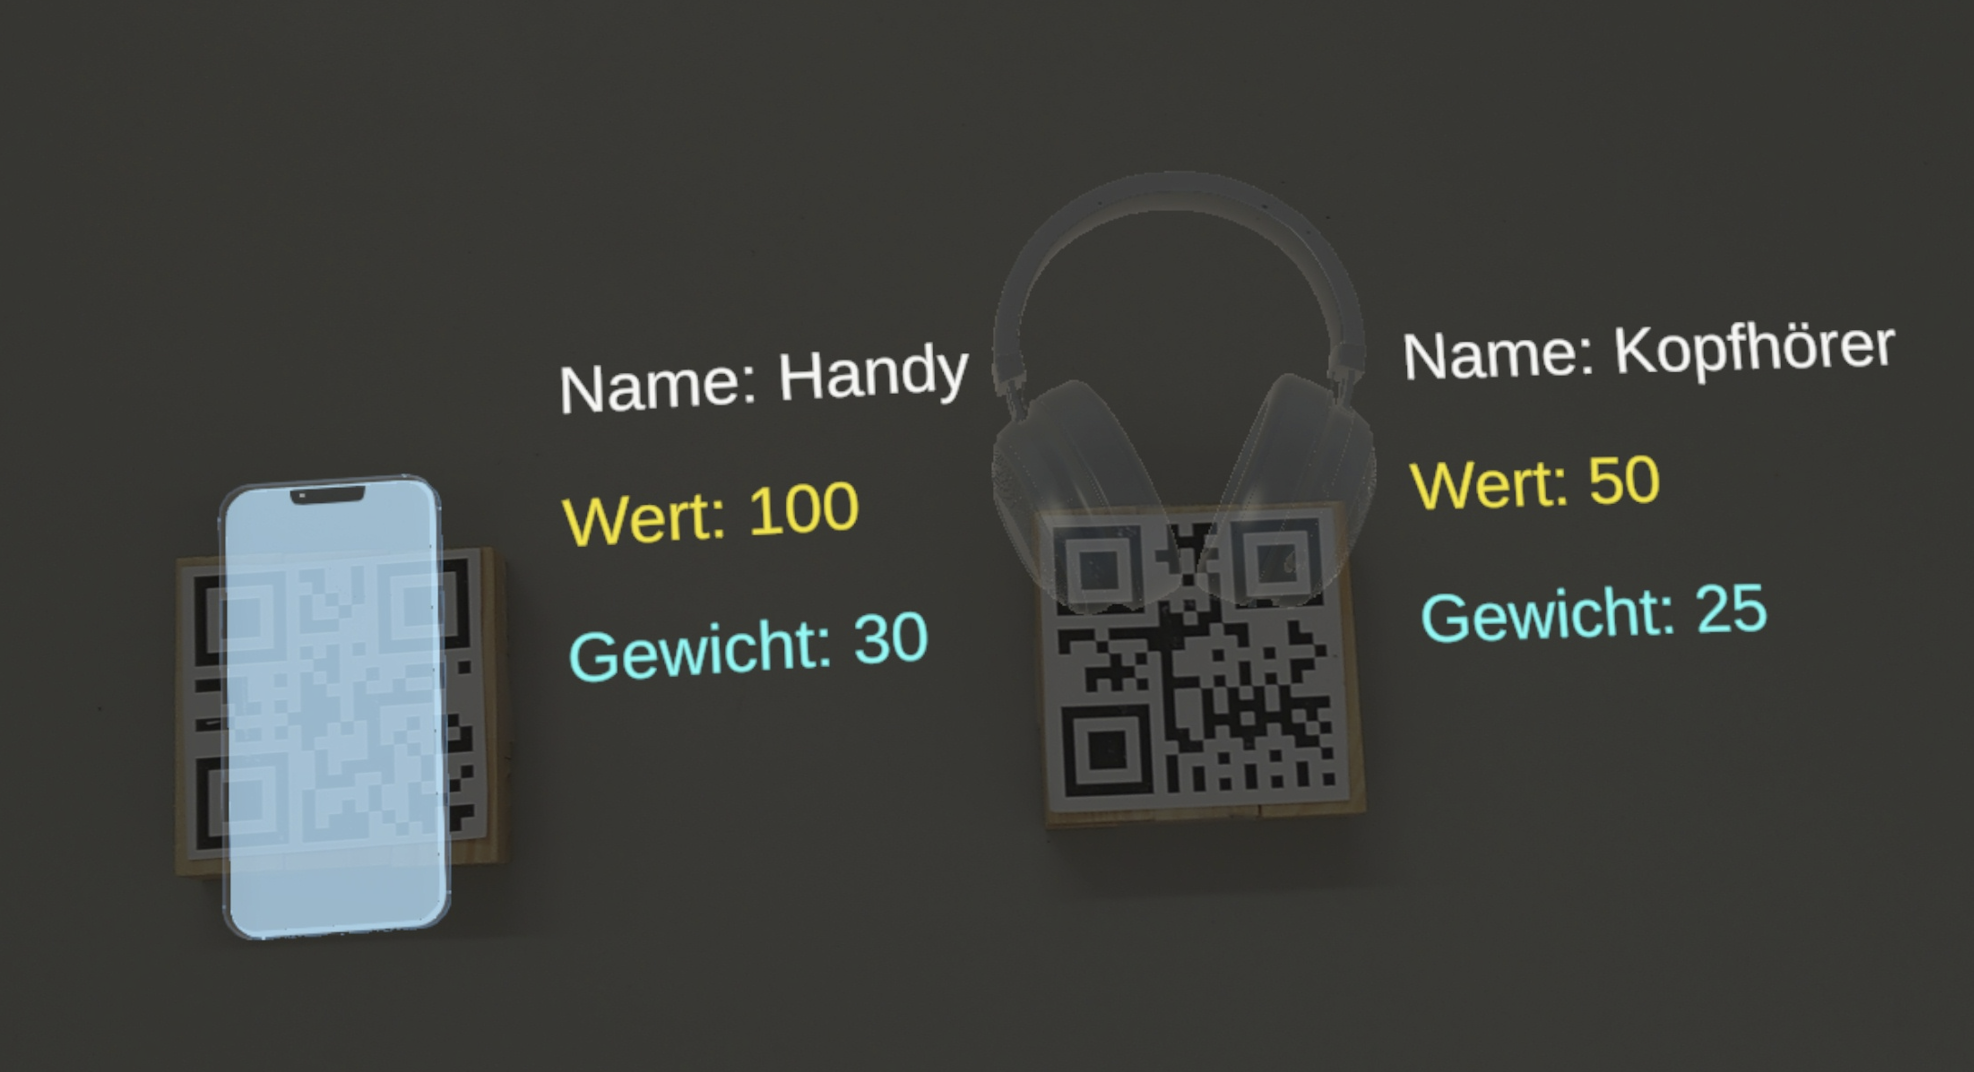
\includegraphics[scale=0.5, angle=0]{images/scanned}
\caption{Visualisierte QR-Codes}
\label{fig:visqr}
\end{figure}

\subsubsection{\label{sec:SGN} Spatial Graph Node}
Ein weiteres wichtiges Konzept, das bei der Übersetzung der Koordinaten verwendet wird, sind sogenannte ``Spatial Graph Nodes``. Diese werden durch das OpenXR-Plugin von Microsoft bereitgestellt und dienen in unserem Fall dazu, die Tracking-Informationen des QR-Codes in der virtuellen Umgebung abzubilden.

Dieses Skript ist mit dem QR-Code-Objekt verbunden und wandelt die Koordinaten des realen QR-Codes in das Unity-Koordinatensystem um. Darüber hinaus platziert das Skript den virtuellen QR-Code im Szenenaufbau genau an derselben Stelle wie den realen QR-Code. Diese Verwendung von Spatial Graph Nodes ermöglicht eine präzise Zuordnung von physischen und virtuellen Objekten in der Mixed-Reality-Umgebung.
%TODO: Quellen


\subsubsection{Zugriff auf QR-Codes bereitstellen}
Wie bereits im Abschnitt \ref{sec:KnapSackProblem} erwähnt, benötigen andere Klassen in der Anwendung Zugriff auf die aktuell erkannten QR-Codes in der Szene, um entsprechend reagieren zu können. Dies ist beispielsweise für die Abfrage erforderlich, ob und welche QR-Codes sich im Inventar befinden. Die Bereitstellung dieser Option war eine Herausforderung.
Um keine Performance-Einbußen auf der Hololens zu verursachen, läuft der Prozess des QR-Code-Trackings auf
mehreren Threads. Die aktuell erkannten QR-Codes werden in einem SortedDictionary gespeichert, welches von anderen Teilen
der Anwendung abgefragt werden kann. Da auf dieses Objekt von mehreren Threads zugegriffen wird, muss es mit einem
\textit{lock} geschützt werden, um Inkonsistenzen zu vermeiden. Hierbei handelt es sich um eine Sperre, die verhindert,
dass mehrere Threads gleichzeitig auf das gleiche Objekt zugreifen. Auf diese Weise wird sichergestellt, dass die Daten
nicht inkonsistent werden und dass die Anwendung stabil und zuverlässig bleibt. Da dadurch bestimten Threads Zugriff verweigert wird (um die Daten zu schützen), kann es zu Verzögerungen kommen, bis die Daten verfügbar sind. Jedoch ist dieser
Nachteil in unserem Anwendungsfall nicht von großer Bedeutung, da wir selten zur gleichen Zeit auf die Daten zugreifen und
dadurch die Verzögerung nicht bemerkbar ist.

\subsection{Platzieren des Inventar Prefabs}\marginpar{\small\(\rightarrow\) {\tiny SKREPEK}}
Eine präzise Interaktion zwischen der realen Welt und der augmentierten Realität erfordert ein tiefgreifendes Verständnis
der Umgebung und eine akkurate Erfassung ihrer Eigenschaften. Um sicherzustellen, dass virtuelle Objekte nahtlos in die
physische Umgebung integriert werden können, ist der Zugriff auf die Kamera unerlässlich. Die Kamera erfasst präzise die
Details der Umgebung, um relevante Ebenen zu identifizieren. Diese sind wichtig für eine präzise Platzierung von virtuellen
Objekten und eine realistische Interaktion zwischen der realen und der augmentierten Welt.

Dieser Abschnitt beschäftigt sich mit der Verwendung des Unity Game Objekts \textit{Inventory Placement Controller} und
dessen angehängter Skript-Komponente. Die \textit{InventoryPlacementController} Klasse bildet die Grundlage für die korrekte
Platzierung des Inventar-Prefabs und gewährleistet einen reibungslosen Ablauf des Anwendungsszenarios des Knapsack-Problems.
Es wird erläutert, wie das Inventar-Prefab strukturiert ist, welche Rolle der User Gaze spielt und wie sie implementiert
wird. Außerdem wird die Logik zur Platzierung des Inventar-Prefabs ausführlich beschrieben.

\subsubsection{Aufbau und Hirarchie des Inventar-Prefabs}
Die Gestaltung und Struktur des Prefabs sind von grundlegender Bedeutung, da dieses Objekt die Basis für die Interaktion
zwischen Benutzer und dem virtuellen Objekt bildet. Eine sorgfältige Ausarbeitung dieses Prefabs trägt wesentlich zur
Gesamterfahrung des Benutzers bei. Es erleichtert dem Benutzer, den Überblick zu behalten, verbessert die Navigation und
fördert eine reibungslose Interaktion. Das Prefab beinhaltet nicht nur ein einfaches Raster zur Darstellung des Inventars,
sondern auch zusätzliche 3D-Modelle, die das Gesamtbild vervollständigen.

\begin{figure}[H]
    \centering
    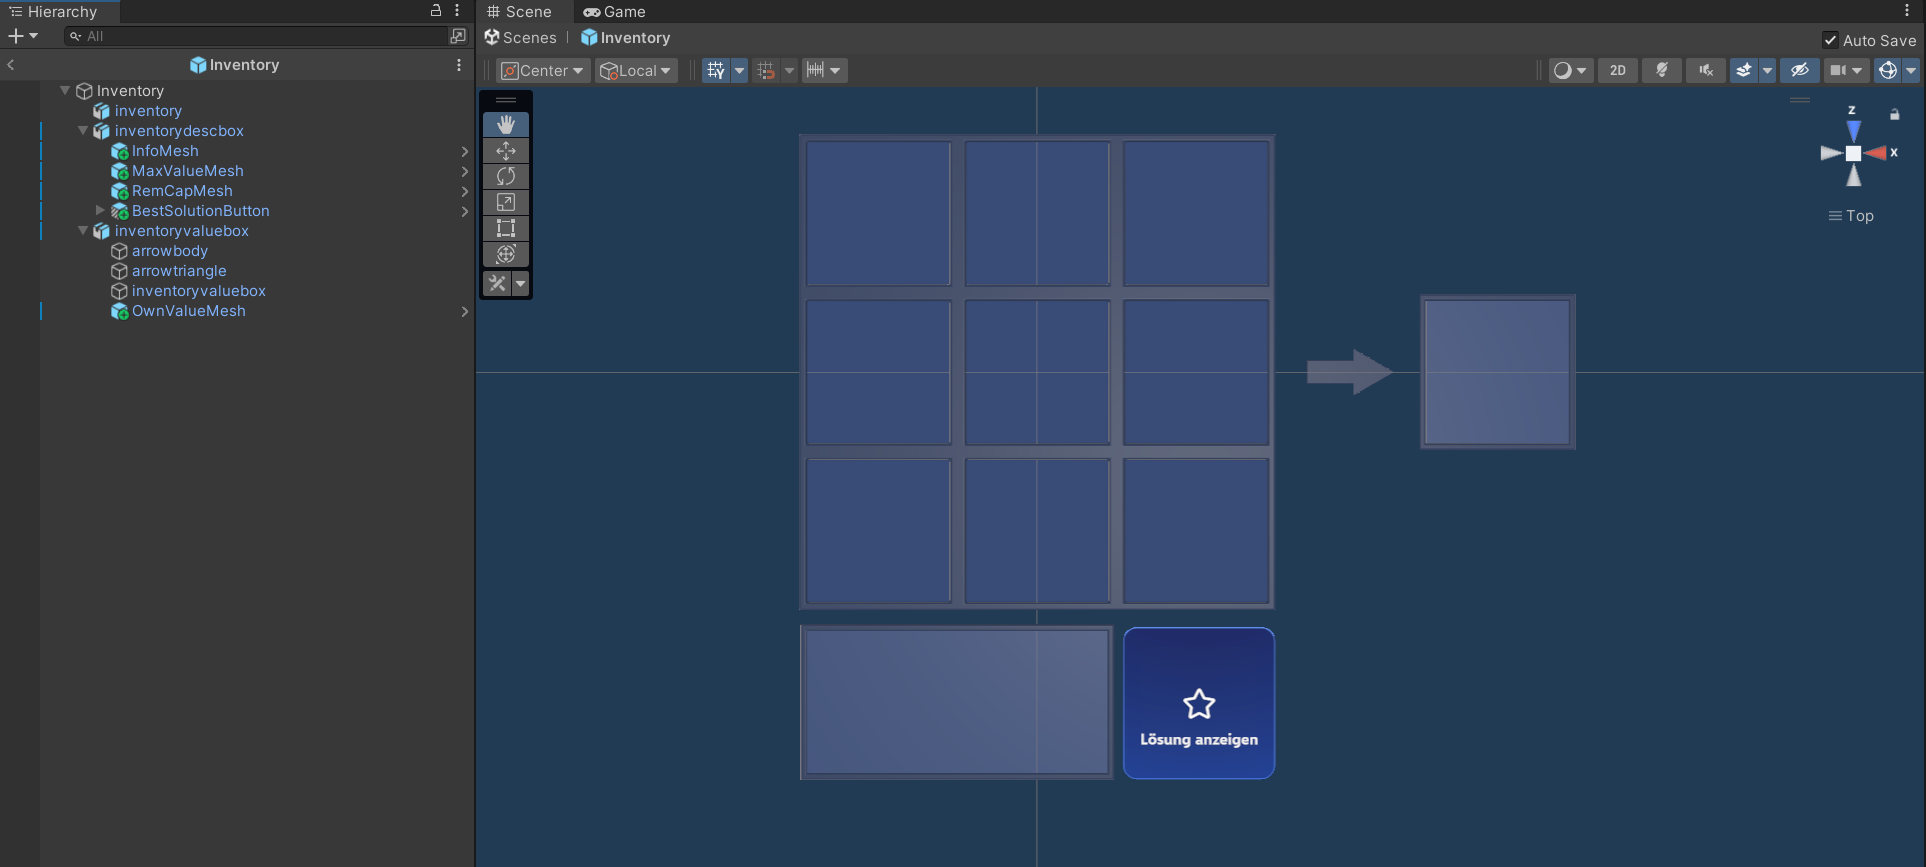
\includegraphics[scale=0.3]{images/invPrefabUnity}
    \caption{Aufbau des Inventar-Prefabs im Unity Editor}
    \label{fig:invPrefab_UNITY}
\end{figure}

Die Abbildung \ref{fig:invPrefab_UNITY} veranschaulicht das gesamte Prefab im Unity Editor und bietet gleichzeitig Einblicke
in die Hierarchie. Es wird deutlich, dass das Prefab aus drei Hauptmodellen besteht, wobei jedes dieser Hauptmodelle weitere
Unterobjekte enthält. Diese drei Hauptmodelle sind:
\begin{enumerate}
    \item \textbf{inventory}: Dieses 3x3-Raster bildet die Hauptkomponente des Prefabs, mit dem der Benutzer interagiert, um
    Gegenstände zu platzieren und zu organisieren.

    \item \textbf{inventorydescbox}: Das Feld unterhalb des Inventar-Rasters gibt dem Benutzer während des Spielverlaufs Feedback.
    Es enthält Warnungen, ob ein Gegenstand zu schwer ist, welcher maximale Wert erreicht werden kann und wie viel Kapazität
    im Inventar noch frei ist. Dem Objekt sind drei \textit{TextMesh}-Elemente untergeordnet. Diese Elemente dienen dazu,
    dem Benutzer das genannte Feedback visuell anzeigen zu können.

    \item \textbf{bestSolutionButton}: Der Knopf neben der \textit{inventorydescbox} ermöglicht dem Benutzer, auf Knopfdruck
    eine perfekte Lösung für das Inventar zu visualisieren. Dadurch kann der Benutzer eine konkrete Vorstellung davon erhalten,
    wie eine solche Lösung aussehen könnte und wie diese im Vergleich zur eigenen Lösung ist. Dies erleichtert die Erkundung
    einer perfekten Anordnung von Gegenständen im Inventar, um gegebenenfalls Anpassungen am eigenen Inventar vorzunehmen.

    \item \textbf{inventoryvaluebox}: Der Pfeil und die Box auf der rechten Seite des Inventars zeigen dem Benutzer an, welchen
    Wert er im Vergleich zum maximal erreichbaren Wert erreicht hat. Diese Information wird durch das Element \textit{TextMesh}
    unterhalb visualisiert. Diese Anzeige ist von großer Bedeutung, da sie dem Benutzer signalisiert, wie effektiv die
    zusammengestellte Lösung ist. Durch die klare Darstellung des aktuellen Werteverhältnisses erhält der Benutzer unmittelbares
    Feedback über die Qualität seiner aktuellen Lösung.
\end{enumerate}

Die Struktur und das Design des Prefabs sind nicht nur ästhetisch ansprechend, sondern auch funktional und im Einklang
mit der übrigen UI/UX der Anwendung. Sie ermöglicht eine effiziente und benutzerfreundliche Interaktion. Die Anordnung
der einzelnen Elemente ist gut durchdacht und bietet dem Benutzer eine klare Orientierung, was die Benutzererfahrung
insgesamt verbessert.

\subsubsection{User Gaze in AR-Anwendungen}
In Augmented-Reality-Anwendungen spielt der \textit{User-Gaze} eine zentrale Rolle, da er die Interaktion zwischen Benutzer
und virtueller Umgebung ermöglicht. Er erfasst und interpretiert dabei die Blickrichtung und -position des Benutzers,
was dessen Aufmerksamkeit in der realen Welt widerspiegelt. Der Gaze ist somit entscheidend, um zu bestimmen, worauf der
Benutzer fokussiert und wie er mit virtuellen Objekten interagiert.

Durch die Verfolgung des User Gazes können in AR-Anwendungen verschiedene Interaktionen ausgelöst werden. Beispielsweise
kann der Benutzer durch einfaches Anschauen eines virtuellen Objekts weitere Informationen anzeigen lassen oder eine
Aktion auslösen. Diese intuitive Form der Interaktion ohne physische Eingabegeräte trägt wesentlich zur Benutzerfreundlichkeit
bei.

Eine präzise Erfassung und Interpretation des Benutzerblicks ist entscheidend für die Realisierung einer nahtlosen und
immersiven AR-Erfahrung. Durch die präzise Verfolgung der Blickrichtung des Benutzers können AR-Anwendungen schnell und
intuitiv auf Benutzeraktionen reagieren. Dadurch wird eine beeindruckende und immersive Interaktion zwischen dem Benutzer
und der virtuellen Umgebung ermöglicht.

\subsubsection{Der Inventory Placement Controller}
Das Unity Game Objekt \textit{Inventory Placement Controller} fungiert als grundlegender Baustein und Ausgangspunkt für
das Anwendungsszenario des Knapsack-Problems. Dieses Objekt übernimmt die Aufgabe dem Benutzer bei Szenenstart Anweisungen
zu vermitteln und das Inventar-Prefab präzise zu platzieren und zu visualisieren. Mit der \textit{InventoryPlacementController.cs}
Skript-Komponente ausgestattet, implementiert dieses Objekt die \textit{InventoryPlacementController} Klasse, welche die
Logik für die Bestimmung des Platzierungsstandorts anhand des Benutzer-Gazes und den weiteren Verlauf dieses Anwendungsszenarios
steuert.

\begin{figure}[H]
    \centering
    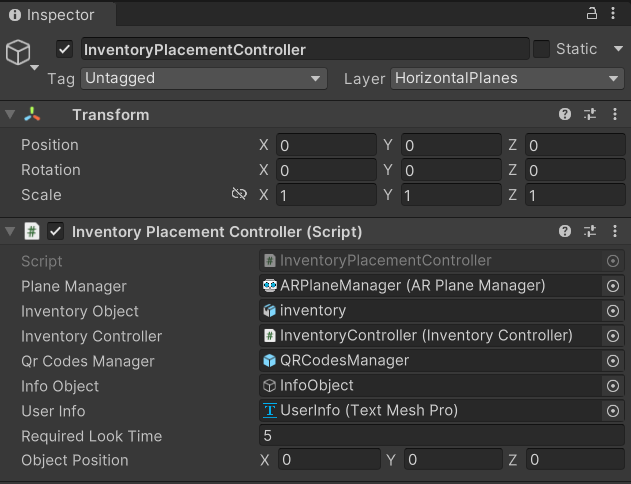
\includegraphics[scale=0.8]{images/invPlace_Editor}
    \caption{Das inventoryPlacementController-Objekt im Unity Editor}
    \label{fig:inventoryPlacementController_Editor}
\end{figure}

Abbildung \ref{fig:inventoryPlacementController_Editor} zeigt das Game Objekt im Unity Inspektor. Ebenfalls zu sehen ist
die angehängte Skript-Komponente, die dem Inventory Placement Controller Game Objekt zugeordnet ist. Innerhalb dieser
Komponente sind die öffentlichen Klassenvariablen des Skripts aufgeführt, die direkt im Inspektor übergeben und manipuliert
werden können. Diese Variablen spielen eine wichtige Rolle bei der Konfiguration und Steuerung des Inventory Placement
Controllers. Zu den relevanten Variablen und ihrer Bedeutung gehören:

\begin{itemize}
    \item \textbf{Inventory Object}: Referenz auf das Inventar Modell aus dem Prefab Ordner, welches platziert werden soll.

    \item \textbf{Inventory Controller}: Verweis auf das Inventory Controller Skript.

    \item \textbf{QR Codes Manager}: Ein Verweis auf das QRCodesManager Game Objekt aus der Szene.

    \item \textbf{User Info}: Referenz auf das in der \texttt{main camera} liegende \textit{TextMesh}.

    \item \textbf{Required Look Time}: Diese Variable definiert die vorgeschriebene Zeit, die der Benutzer auf eine
    Fläche blicken muss, um das Inventar darauf zu platzieren.

    \item \textbf{Object Position}: Variable, in der die Platzier-Position des Inventars gespeichert wird, um später
    darauf zugreifen zu können.
\end{itemize}

Die korrekte Übergabe und Konfiguration dieser Objekte und Werte an das Unity Game Objekt sind entscheidend für die
gewünschte und korrekte Funktionsweise des Platzierungsvorgangs des Inventar-Prefabs. Durch die Anpassung der Variablen
und ihrer Werte kann die Platzierungsdynamik präzise gesteuert werden, um eine reibungslose Benutzererfahrung zu gewährleisten.

\subsubsection{Implementierung des User Gazes}
Im Falle des Knapsack-Anwendungsszenarios wird der Gaze des Benutzers genutzt, um festzustellen, ob dieser auf eine durch
den \textit{AR Plane Manager} erfasste Ebene (\textit{AR-Plane}) gerichtet ist. Diese Feststellung ist von großer Bedeutung,
um zu bestimmen, ob der Benutzer auf eine geeignete Fläche blickt, auf der das Inventar-Prefab platziert werden kann.
Die Klasse \textit{InventoryPlacementController} verwendet zwei Funktionen, um den Blick des Benutzers auf ein \textit{ARPlane}
zu erkennen und, um dieses \textit{ARPlane} zu ermitteln und zurückzugeben. In diesem Abschnitt wird die Funktion, welche
den Blick-Status ermittelt, anhand des Source-Codes erklärt.
\begin{lstlisting}[caption={Funktion zur Überprüfung des User Gazes}, label=code:isPOP]
private bool IsPointerOverPlane() {
    Ray ray = Camera.main.ScreenPointToRay(Input.mousePosition);
    RaycastHit hit;
    if (Physics.Raycast(ray, out hit)) {
        ARPlane plane = hit.collider.GetComponent<ARPlane>();
        return (plane != null);
    }
    return false;
}
\end{lstlisting}
Um den Status des User Gazes zu überprüfen und damit festzustellen, ob der Benutzer auf ein AR-Plane blickt, wird ein
Strahl aus der Hauptkamera (\texttt{Camera.main}) in Richtung der aktuellen \textit{Blickrichtung} und \textit{Position}
des Benutzers geschossen. Wenn dieser Strahl mit einem virtuellen Objekt in der Szene kollidiert, wird überprüft, ob es
sich bei dieser Kollision um ein AR-Plane handelt.

Diese Überprüfung erfolgt über den Zugriff auf die Kollisionskomponente (\texttt{collider}) des getroffenen Objekts
(\texttt{hit}), um auf die spezifische Komponente AR-Plane zuzugreifen. Wenn das getroffene Objekt als AR-Plane identifiziert
werden kann, gibt die Funktion \texttt{true} zurück, woraus geschlossen werden kann, dass der Benutzer seinen Blick auf
ein AR-Plane gerichtet hat. Ansonsten gibt diese Funktion \texttt{false} zurück, was das Gegenteil bedeutet.

\subsubsection{Platzierungskontrolle und ARPlane-Überwachung}
Da der Benutzer während des Platzierungsvorgangs möglicherweise seine Blickrichtung ändert, ist es wichtig, die kontinuierlich
zu überprüfen, oder ob ein neues AR-Plane im Fokus des Benutzers liegt. Diese fortlaufende Überprüfung ist entscheidend,
um sicherzustellen, dass bei einer Änderung des Blicks das neue im Fokus liegende AR-Plane ausgewählt wird und der Vorgang
reibungslos fortgesetzt werden kann. Um diese Funktionalität zu realisieren, wird die Funktion \texttt{Update()} verwendet.

Diese Funktion ist von entscheidender Bedeutung, da sie sicherstellt, dass der aktuelle Stand des User Gazes kontinuierlich
überprüft wird. Dadurch wird gewährleistet, dass das Inventar-Prefab präzise platziert werden kann, selbst wenn sich die
Blickrichtung des Benutzers ändert. Um die Logik, die diesem Prozess zugrunde liegt, zu veranschaulichen, wird im Folgenden
der Source-Code erklärt.
\begin{lstlisting}[caption={Funktion um Usergaze zu verwenden}, label=code:isPOP]
void Update() {
    if (!objectPlaced && canStartScript) {
        if (IsPointerOverPlane()) {
            ARPlane currentPlane = GetCurrentPlaneUnderGaze();
            if (currentPlane != null) {
                if (selectedDeskPlane == null || selectedDeskPlane != currentPlane) {
                    selectedDeskPlane = currentPlane;
                    lookStartTime = Time.time;
                }
                float timeLookedAtPlane = Time.time - lookStartTime;
                userInfo.text = ((int)requiredLookTime - (int)timeLookedAtPlane).ToString();
                if (timeLookedAtPlane >= requiredLookTime) {
                    PlaceObjectOnDesk(selectedDeskPlane);
                    objectPlaced = true;
                    userInfo.text = "";
                }
            } else {
                selectedDeskPlane = null;
                userInfo.text = "Schauen Sie auf einen Tisch";
            }
        } else {
            selectedDeskPlane = null;
            userInfo.text = "Schauen Sie auf einen Tisch";
        }
    }
}
\end{lstlisting}\\
Generell lässt sich die Funktionsweise dieses Codes in neun Phasen unterteilen, um das Inventar-Prefab entgültig zu platzieren. Diese Phasen sind:

\begin{enumerate}
    \item \textbf{Platzierungsstatus und Skript-Startbedingung}: Zunächst wird überprüft, ob das Prefab für das Inventar
    noch nicht platziert wurde (\texttt{objectPlaced}) und, ob das Skript gestartet werden kann (\texttt{canStartScript}).
    Dies gewährleistet, dass die Platzierung nur erfolgt, wenn beide Bedingungen erfüllt sind.

    \item \textbf{Bestimmung des User Gazes über einem AR-Plane}: Anschließend wird geprüft, ob sich der User Gaze über einem
    AR-Plane befindet. Hierfür wird die Funktion \texttt{IsPointerOverPlane()} aufgerufen, welche feststellt, ob sich der
    Benutzergaze über einem AR-Plane befindet.

    \item \textbf{Identifikation des aktuellen ARPlane}: Wenn bestätigt wird, dass sich der User Gaze über einem AR-Plane
    befindet, wird das aktuelle AR-Plane identifiziert. Hierfür wird die Funktion \texttt{GetCurrentPlaneUnderGaze()} aufgerufen,
    welche das AR-Plane bestimmt, auf den der Benutzergaze gerichtet ist.

    \item \textbf{AR-Plane aktualisieren und Timer starten}: Nach Identifikation des AR-Planes wird überprüft, ob es sich um
    ein anderes AR-Plane als dieses handelt, auf welches der Benutzer zuletzt geschaut hat. Falls dies der Fall ist, wird
    die Variable \texttt{selectedDeskPlane} aktualisiert und die Startzeit des Blicks auf dem neuen AR-Plane wird gespeichert.

    \item \textbf{Messung der Blickdauer und Anzeige der Zeit}: Es wird die Dauer gemessen, die der Benutzer bereits auf das
    aktuelle AR-Plane blickt. Hierfür wird die Zeitdifferenz seit dem Start des Blicks auf dieses AR-Plane berechnet.
    Zusätzlich wird dem Benutzer mittels des TextMeshes \texttt{userInfo} in Form eines \textit{Countdowns} angezeigt, wie
    lange er noch auf dieses ARPlane blicken muss.

    \item \textbf{Erforderte Blickdauer erreicht}: Es wird überprüft, ob die gemessene Zeit die erforderliche Zeit
    überschreitet, die der Benutzer benötigt, um das Inventar-Prefab auf dem AR-Plane zu platzieren.

    \item \textbf{Platzierung des Inventar Prefabs}: Nachdem die erforderliche Blickdauer erreicht wurde, wird die Funktion
    \texttt{PlaceObjectOnDesk()} (siehe Codeabschnitt \ref{code:placeObject}) aufgerufen, um das Inventar-Prefab auf dem
    ausgewählten AR-Plane zu platzieren. (siehe Abschnitt \ref{sec:platzierungsablauf})

    \item \textbf{Platzierungsstatus}: Nachdem das Objekt erfolgreich platziert wurde, wird die Variable \texttt{objectPlaced}
    auf true gesetzt, um anzuzeigen, dass das Objekt platziert wurde.

    \item \textbf{Benachrichtigung bei fehlendem AR-Plane}: Wenn sich der User Gaze nicht über einem AR-Plane befindet oder
    kein AR-Plane erkannt wird, wird die Benutzeroberfläche entsprechend aktualisiert. Der Benutzer wird darüber informiert,
    dass er auf ein AR-Plane blicken muss, um das Inventar-Prefab erfolgreich zu platzieren.
\end{enumerate}

\subsubsection{Platzierung des Prefabs}
Die Platzierung des Inventar-Prefabs markiert den Abschluss des Skripts \textit{Inventory Placement Controllers}. Die
Funktion \texttt{PlaceObjectOnDesk()} platziert das Prefab auf dem ARPlane, auf welches der Benutzer blickt und aktiviert
bzw. deaktiviert weitere Game Objekte sowie Skripte, um einen nahtlosen Fortlauf der Anwendung zu gewährleisten.
\begin{lstlisting}[caption={Funktion zum Platzieren des Inventarobjekts}, label=code:placeObject]
    private void PlaceObjectOnDesk(ARPlane deskPlane) {
    qrCodesManager.SetActive(true);
    objectPosition = deskPlane.center + Vector3.up * heightOffset;
    wholeInventory.transform.position = objectPosition;
    wholeInventory.transform.rotation = Quaternion.Euler(0, 180f, 0);
    wholeInventory.SetActive(true);
    GameObject inventory = wholeInventory.transform.Find("inventory").gameObject;
    inventoryController.SetInventoryObject(inventory);
    inventoryController.gameObject.SetActive(true);
    gameObject.SetActive(false);
}
\end{lstlisting}

Die Platzierung des Inventar-Prefabs erfolgt in vier Hauptschritten, die den Ablauf des Platzierungsprozesses steuern
und die Kontinuität des AR-Anwendungsszenarios sicherstellen.

\begin{enumerate}
    \item \textbf{Aktivierung des QRCodesManagers:} Der QRCodesManager wird aktiviert, um sicherzustellen, dass QR-Codes
    nach Abschluss dieses Skripts erfolgreich erfasst werden können.

    \item \textbf{Berechnung der Position und Rotation:} Die Position des Inventar-Prefabs auf dem AR-Plane wird berechnet,
    um sicherzustellen, dass es an der richtigen Stelle platziert wird. Die Rotation des Objekts wird angepasst, um eine
    korrekte Ausrichtung zu gewährleisten. Schließlich wird das Objekt aktiviert, um es für den Benutzer sichtbar zu machen.

    \item \textbf{Extraktion und Übergabe des Inventar-Objekts:} Das Inventar-Objekt wird aus dem Prefab extrahiert und an
    den \textit{Inventory Controller} übergeben. Dadurch wird eine nahtlose Fortsetzung der Interaktion mit dem Inventar ermöglicht.

    \item \textbf{Deaktivierung des Objekts:} Abschließend wird das eigene Game-Objekt deaktiviert, um das Ende des
    Platzierungsvorgangs des Inventar-Prefabs zu markieren. Dadurch wird dem Benutzer signalisiert, dass der Platzierungsvorgang
    abgeschlossen ist und eine klare Abgrenzung erleichtert.
\end{enumerate}

Diese Schritte sind essenziell für einen reibungslosen Ablauf des Platzierungsprozesses des Inventar-Prefabs und tragen
zu einer effizienten und benutzerfreundlichen Interaktion innerhalb des AR-Anwendungsszenarios bei.

\subsubsection{Visualisierung des Platzierungsablaufs}\label{sec:platzierungsablauf}
Um den Prozess des Platzierens des Inventar-Prefabs aus der Perspektive des Benutzers besser zu veranschaulichen, werden
in den folgenden drei Abbildungen \ref{fig:eins}, \ref{fig:zwei} und \ref{fig:drei} die Schritte dieses Vorgangs dargestellt.
Dabei illustriert die letzte Abbildung \ref{fig:drei} den Endzustand mit dem platzierten Inventar sowie einer darauf
folgenden Anweisung für den Benutzer.

Diese visuelle Darstellung bietet eine ergänzende Perspektive auf den Ablauf des Platzierens und ermöglicht es, die
einzelnen Schritte des Prozesses besser zu verstehen und den Abschluss des Platzierungsvorgangs nachzuvollziehen.

\begin{figure}[H]
    \centering
    \begin{minipage}[b]{0.30\textwidth}
        \centering
        
\includegraphics[width=\textwidth]{images/schritteins.png}
        \label{fig:eins}
    \end{minipage}
    \hfill
    \begin{minipage}[b]{0.30\textwidth}
        \centering
        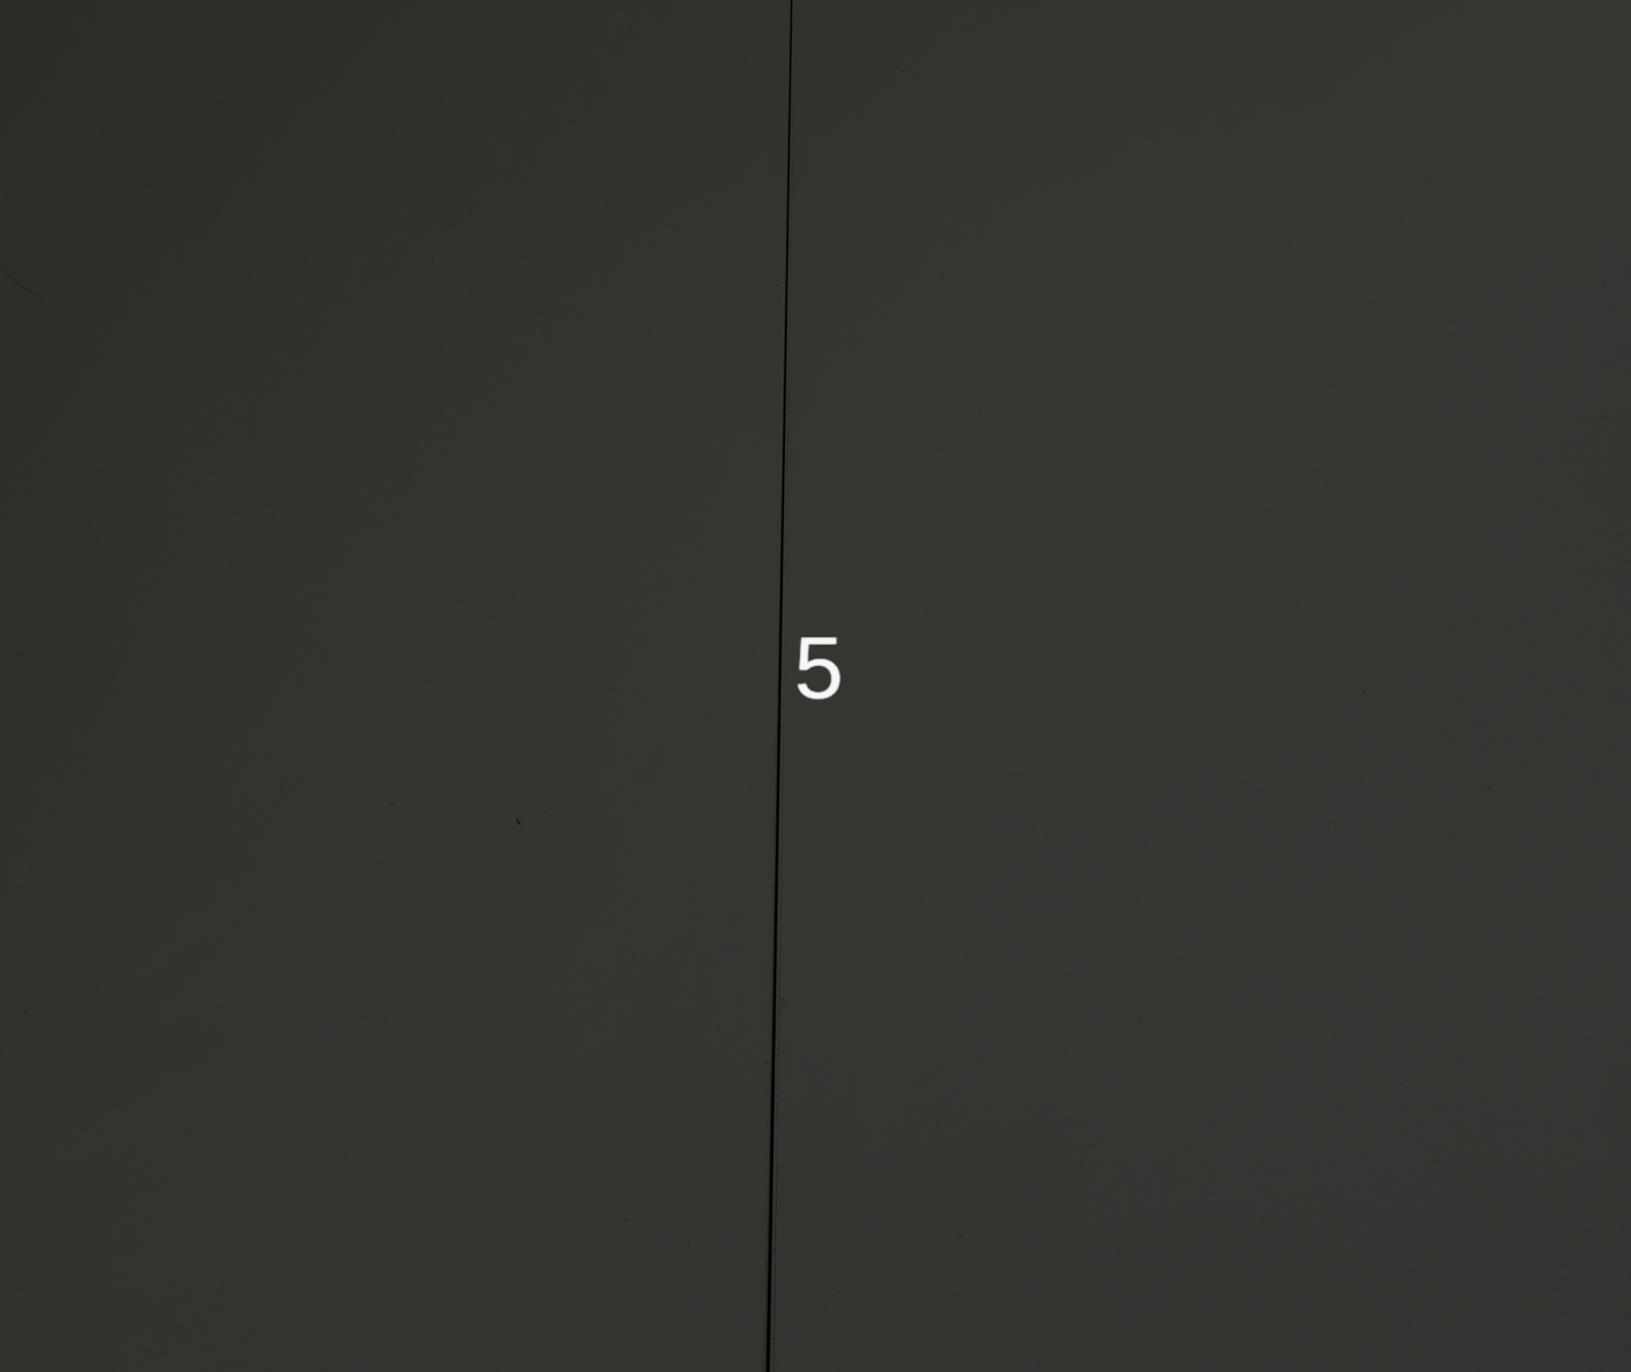
\includegraphics[width=\textwidth]{images/schrittzwei.png}
        \label{fig:zwei}
        \end{minipage}
    \hfill
    \begin{minipage}[b]{0.30\textwidth}
        \centering
        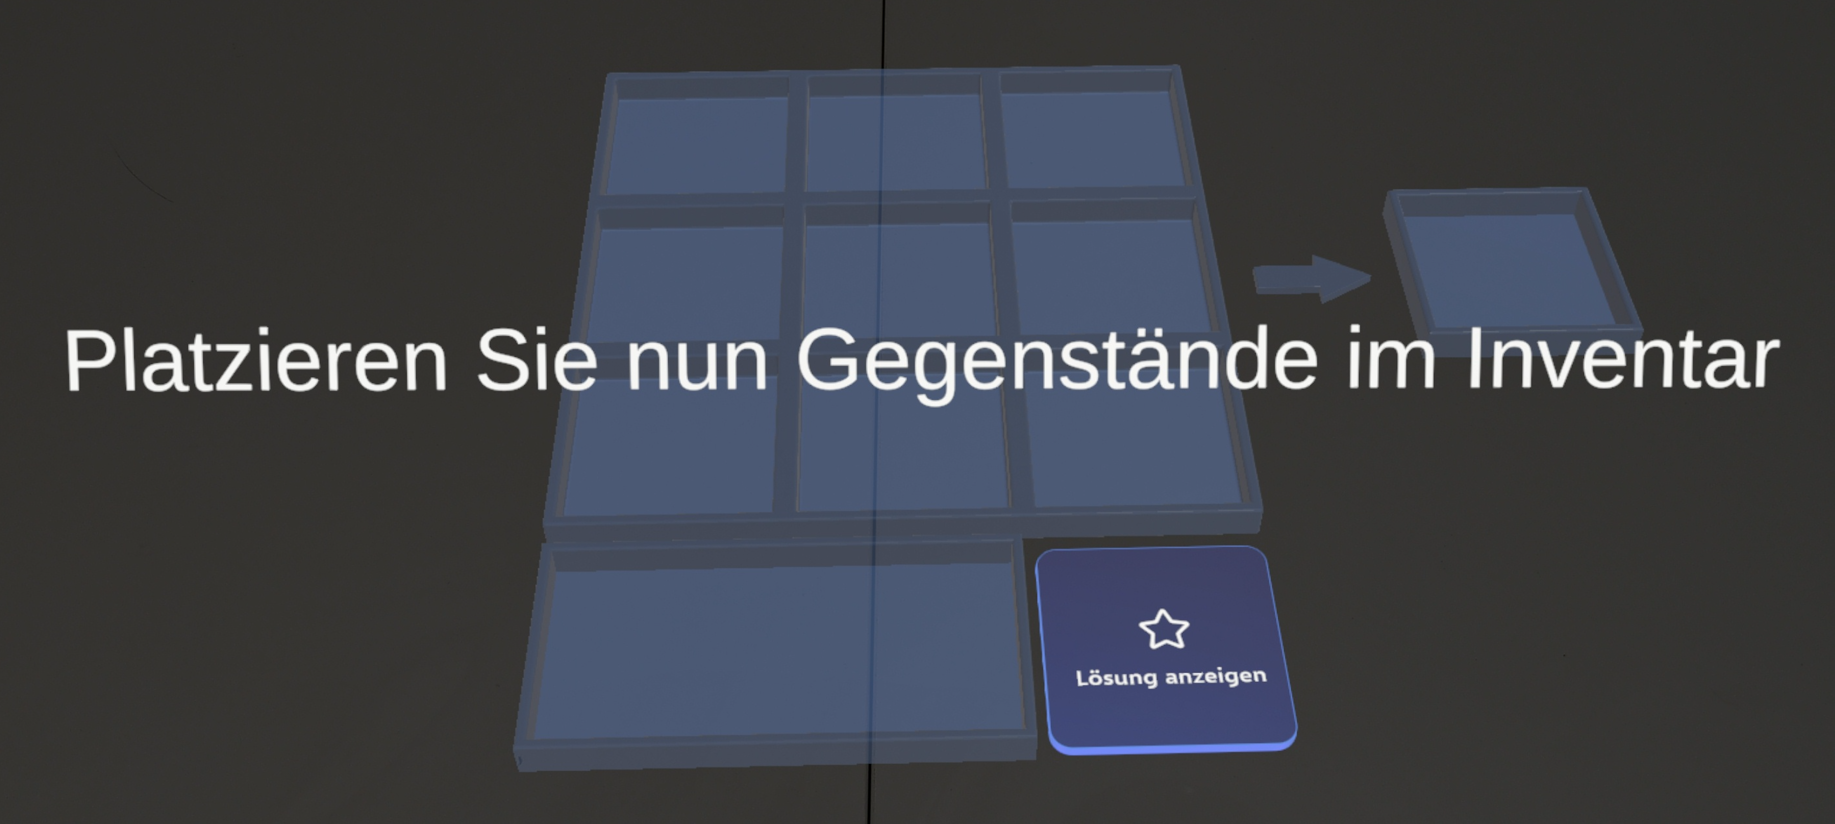
\includegraphics[width=\textwidth]{images/schrittdrei.png}
        \label{fig:drei}
    \end{minipage}
\end{figure}

Die erste Abbildung zeigt, dass der Benutzer zu diesem Zeitpunkt nicht auf eine horizontale Fläche blickt. Daraufhin
wird eine Anweisung angezeigt, dass auf eine horizontale Fläche geblickt werden muss, um das Inventar-Prefab platzieren
zu können. Diese Anweisung dient als Orientierungshilfe, um den ersten Schritt des Platzierungsprozesses erfolgreich
abzuschließen.

Die zweite Abbildung zeigt, dass der Benutzer seinen Blick nun auf einen Tisch, d.h. eine horizontale Fläche, gerichtet
hat. Diese Aktion startet einen Countdown, der dem Benutzer visuell anzeigt, wie lange er noch auf diese Fläche blicken
muss, um das Inventar-Prefab erfolgreich zu platzieren.

Die dritte Abbildung zeigt den Abschluss des Platzierungsprozesses, bei dem das Inventar-Prefab erfolgreich platziert
wurde. Nach Abschluss dieser Phase erhält der Benutzer weitere Anweisungen für die nächsten Schritte, um das Inventar
effektiv im Spiel zu verwenden.

\subsection{Inventarverwaltung}\marginpar{\small\(\rightarrow\) {\tiny SKREPEK}}
Eine effiziente Handhabung und Überwachung des platzierten Inventars ist ein zentraler Aspekt im Kontext des Rucksack-Problems.
Es ist wichtig, das Inventar fortlaufend und präzise in Echtzeit zu erfassen und zu aktualisieren, um sämtliche Veränderungen -
sei es das Hinzufügen oder Entfernen eines Gegenstands seitens des Benutzers - unmittelbar zu registrieren. Dank dieses
Echtzeit-Feedbacksystems ist es möglich, direkt auf Veränderungen zu reagieren und dem Benutzer entsprechendes Feedback zu geben.

Dieser Abschnitt beschreibt das \textit{Inventory Controller} Unity Game Objekt und seine angehängte Skript-Komponente
im Detail. Die Klasse \textit{InventoryController} ist das Herzstück für die Überwachung und Verwaltung des Inventars
und gewährleistet einen reibungslosen und kontinuierlich aktualisierten Ablauf des Anwendungsszenarios des Rucksack-Problems
in Echtzeit. Es wird erläutert, wie diese Klasse funktioniert und welche Bedeutung die Begrenzungen eines Objekts in
diesem Kontext haben.

\subsubsection{Der Inventory Controller}
Das Unity Game Objekt \texttt{Inventory Controller} ist von entscheidender Bedeutung für die nahtlose Interaktion und
Kontrolle des Inventars innerhalb des Anwendungsszenarios des Rucksack-Problems. Diese zentrale Einheit fungiert als Dreh-
und Angelpunkt für die Erfassung und Verarbeitung sämtlicher Änderungen am Inventar, die durch den Benutzer initiiert
werden. Ausgestattet mit der Skript-Komponente \textit{InventoryController.cs}, verkörpert das \textit{Inventory Controller}
Objekt die \textit{InventoryController} Klasse, welche nicht nur die Verwaltung des Inventars, sondern auch dessen
Echtzeitüberwachung steuert. Diese Klasse bildet das Rückgrat für die reibungslose und kontinuierliche Aktualisierung
des Inventars gemäß den Handlungen des Benutzers.

\begin{figure}[H]
    \centering
    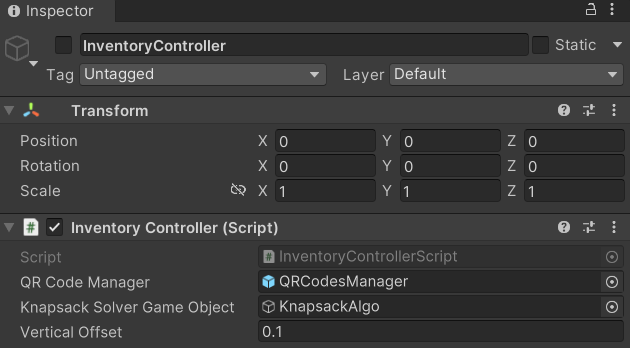
\includegraphics[scale=0.7]{images/invCon_Editor}
    \caption{InventoryController Objekt im Editor}
    \label{fig:InventoryController_Editor}
\end{figure}

Abbildung \ref{fig:InventoryController_Editor} zeigt das Game Objekt im Unity Inspektor, welches den Inventory Controller
repräsentiert. Es ist erkennbar, dass diesem Objekt eine Skript-Komponente angehängt ist, die dem Inventory Controller
zugeordnet ist. Innerhalb dieser Komponente werden die öffentlichen Klassenvariablen des Skripts aufgeführt, welche direkt
im Inspektor eingesehen und manipuliert werden können. Diese Variablen sind wichtig für die Konfiguration und Steuerung
des Inventory Controllers. Folgende Variablen sind relevant und haben eine bestimmte Bedeutung:

\begin{itemize}
    \item \textbf{QR Code Manager}: Referenz auf das \textit{QRCodeManager} Game Objekt aus der Szene.

    \item \textbf{Knapsack Solver Game Objekt}: Ein Verweis auf das \textit{KnapsackSolver} Game Objekt aus der Szene.

    \item \textbf{User Info}: Referenz auf das in der \textit{main camera} liegende \textit{TextMesh}.

    \item \textbf{Vertical Offset}: Float-Wert, um den die Begrenzungen (\textit{Bounds}) des Inventory-Objekts auf
    der X-Achse erweitert werden.
\end{itemize}

Die korrekte Übergabe und Konfiguration dieser Objekte und Werte an das Unity Game Objekt ist von entscheidender Bedeutung
für die gewünschte und fehlerfreie Funktionsweise der Inventarverwaltung. Durch die Anpassung dieser Werte und Variablen
lässt sich das Verhalten der Verwaltungsdynamik präzise steuern, um eine nahtlose Benutzererfahrung sicherzustellen.

\subsubsection{Begrenzungen eines Objekts}
Die Begrenzungen eines Objekts, auch als \textit{Bounds} bezeichnet, sind ein essenzielles Konzept in der Computerspielentwicklung
und anderen Bereichen der Computergrafik. Sie definieren den umschließenden \textit{Raum} oder \textit{Bereich}, den ein
Objekt einnimmt. Diese Begrenzungen sind von grundlegender Bedeutung für die räumliche Positionierung von Objekten sowie
für die Kollisions- und Interaktionsprüfung zwischen verschiedenen Elementen innerhalb einer Szene.\footnote{Unity Dokumentation \cite{Bounds}}

In Unity werden die Begrenzungen eines Objekts über die Eigenschaften der Klasse \textit{Bounds} verwaltet. Jedes Game
Objekt in Unity ist mit einer \textit{Collider}-Komponente ausgestattet, der unter anderem die Begrenzungen des Objekts
definiert. Die ermittelten Begrenzungen eines Objekts haben eine Vielzahl von Anwendungsbereichen:

\begin{enumerate}
    \item \textbf{Kollisionserkennung:} Durch den Vergleich der Begrenzungen zweier Objekte können Kollisionen zwischen
    diesen erkannt werden. Dieser Prozess ist von grundlegender Bedeutung für die physikalische Interaktion von Objekten
    innerhalb einer digitalen Umgebung und ermöglicht die Umsetzung realistischer Verhaltensweisen.

    \item \textbf{Platzierung von Objekten:} Die Begrenzungen dienen als Leitfaden für die Platzierung neuer Objekte
    innerhalb einer Szene. Durch die Gewährleistung, dass die Positionierung innerhalb eines definierten Bereichs oder
    Umfelds erfolgt, wird die konsistente Gestaltung und Strukturierung der digitalen Welt ermöglicht.

    \item \textbf{Bewegung und Rotation von Objekten:} Bei der Bewegung oder Rotation von Objekten können die Begrenzungen
    genutzt werden, um sicherzustellen, dass diese innerhalb eines vordefinierten Gültigkeitsbereichs bleiben. Dies
    gewährleistet nicht nur die Kohärenz der Szene, sondern auch die Vermeidung von unerwünschten Interferenzen oder
    Überschneidungen zwischen verschiedenen Elementen.
\end{enumerate}

Die effektive Nutzung der Begrenzungen eines Objekts trägt somit wesentlich zur Präzision und Stabilität digitaler
Szenen bei, indem sie eine solide Grundlage für die Positionierung, Bewegung und Interaktion von Objekten innerhalb
einer virtuellen Umgebung bildet.

\subsubsection{Problem bei Standardbegrenzungen}
Die Standardbegrenzungen des Inventar-Objekts sind so festgelegt, dass sie genau die räumliche Fläche dieses Objekts
abdecken. Dies kann jedoch zu Problemen führen, insbesondere wenn sich ein Gegenstand innerhalb dieser Grenzen befindet,
aber möglicherweise nicht erkannt wird. Dies tritt auf, weil die QR-Codes auf realen Objekten (Holzplättchen mit einer
Stärke / Höhe von 20 mm) angebracht sind und daher die Position entlang der y-Achse (Höhe) verschoben wird.

Um dieses Problem zu lösen, müssen die Begrenzungen erweitert werden. Dies ermöglicht es dem \textit{Inventory Controller},
auch Gegenstände zu erfassen, die sich möglicherweise innerhalb des ursprünglichen Begrenzungsbereichs befinden, aber
aufgrund der vertikalen Verschiebung nicht erkannt wurden. Durch die Erweiterung der Grenzen wird sichergestellt, dass
alle relevanten Objekte ordnungsgemäß erfasst und im Inventar berücksichtigt werden.

Diese Erweiterung der Begrenzungen ist insbesondere wichtig, um die Zuverlässigkeit und Effizienz des \textit{Inventory Controller}
sicherzustellen, insbesondere in Umgebungen, in denen die vertikale Positionierung der Objekte variiert und demnach eine
präzise Erfassung erforderlich ist.

\subsubsection{Erweitern der Standardbegrenzungen}
Um das Problem der Nichterkennung von neu hinzugefügten Gegenständen im Inventar aufgrund der Begrenzungen des Inventar-Objekts
zu lösen, müssen die Standardbegrenzungen des Objekts gründlich überprüft und erweitert werden. Dieser Schritt wird
durch die sorgfältige Implementierung der Funktion \texttt{UpdateInventoryBounds()} realisiert. Diese Funktion ermöglicht
es, die Grenzen des Inventar-Objekts anzupassen und entsprechend der aktuellen Anforderungen zu erweitern.

Die Herausforderung besteht darin, sicherzustellen, dass das Inventar sämtliche neu hinzugefügten Gegenstände korrekt
erkennt und effizient verwaltet, selbst wenn diese die ursprünglichen Begrenzungen des Objekts überschreiten. Durch die
Aktualisierung der Standardbegrenzungen können solche Änderungen sofort erfasst und berücksichtigt werden, wodurch ein
unterbrechungsfreier Ablauf des \textit{Inventory Controllers} gewährleistet wird.

Die Funktion besteht aus drei Phasen, die durchlaufen werden, um die Begrenzungen des Objekts zu erweitern. Diese sind d
ie folgenden:

\begin{enumerate}
\item \texttt{UpdateInventoryBounds()}: Diese Funktion ist die zentrale Methode, die aufgerufen wird, um die Begrenzungen
des Inventars zu aktualisieren. Sie überprüft zunächst, ob ein Inventarobjekt vorhanden ist und ruft anschließend
Hilfsfunktionen auf, um den Rest abzuarbeiten. Die Begrenzungen werden entsprechend des vertikalen Versatzes erweitert.
\begin{lstlisting}[language={[Sharp]C}]
private void UpdateInventoryBounds() {
if (inventoryObject != null) {
Bounds localBounds = GetBounds(inventoryObject);
ExtendBounds(ref localBounds, verticalOffset);
inventoryBounds = localBounds;
}
}
\end{lstlisting}

\item \texttt{GetBounds()}: Diese Methode dient dazu, die Grenzen des übergebenen Spielobjekts zu bestimmen. Sie verwendet
die Renderer-Komponenten des Objekts, um die Grenzen zu erhalten, und fällt auf die Position des Objekts zurück, falls
kein Renderer vorhanden ist.
\begin{lstlisting}[language={[Sharp]C}]
private Bounds GetBounds(GameObject obj) {
Renderer renderer = obj.GetComponent<Renderer>();
return renderer != null ? renderer.bounds : new Bounds(obj.transform.position, Vector3.one);
}
\end{lstlisting}

\item \texttt{ExtendBounds()}: Hier handelt es sich um die Funktion, die die eigentliche Erweiterung der Begrenzungen
durchführt. Durch die Verwendung einer Referenz ist es möglich, direkt die Begrenzungen des originalen Objekts zu
bearbeiten. Sie passt sowohl das Zentrum als auch die Ausdehnung der Begrenzung auf der y-Achse entsprechend des \texttt{offset} an.
\begin{lstlisting}[language={[Sharp]C}]
private void ExtendBounds(ref Bounds bounds, float offset) {
bounds.center = new Vector3(bounds.center.x, bounds.center.y + offset / 2, bounds.center.z);
bounds.extents = new Vector3(bounds.extents.x, bounds.extents.y + offset / 2, bounds.extents.z);
}
\end{lstlisting}
\end{enumerate}

Diese Funktionen stellen sicher, dass die Begrenzungen des Inventars aktualisiert werden, um sicherzustellen, dass alle
relevanten Objekte ordnungsgemäß erfasst und berücksichtigt werden. Dies trägt dazu bei, die Zuverlässigkeit und Effizienz
des \textit{Inventory Controllers} zu verbessern, insbesondere in Umgebungen, in denen die vertikale Position der Objekte
variiert.

\subsubsection*{Vorher-Nachher-Vergleich der Begrenzungen}
Um den Effekt der Funktion \texttt{UpdateInventoryBounds()} auf die Begrenzungen des Objekts zu verdeutlichen, werden
in den folgenden Abbildungen der Zustand vor und nach dem Aufruf der Funktion gegenübergestellt.

\begin{figure}[H]
    \centering
    \begin{minipage}[b]{0.45\textwidth}
        \centering
        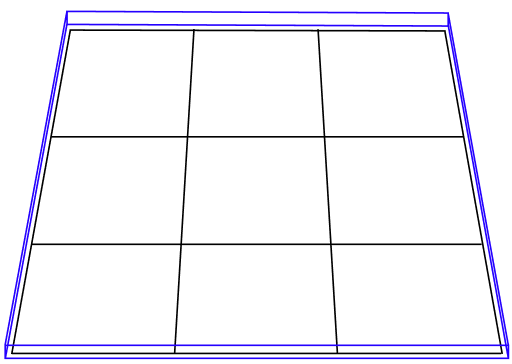
\includegraphics[width=\textwidth]{vorher.png}
        \caption{Begrenzungen vor dem Funktionsaufruf}
        \label{fig:voraufr}
    \end{minipage}
    \hfill
    \begin{minipage}[b]{0.45\textwidth}
        \centering
        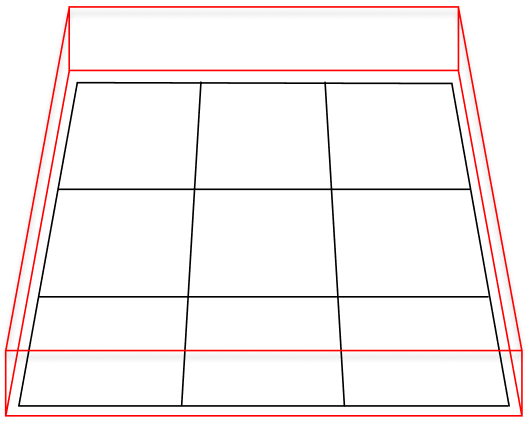
\includegraphics[width=\textwidth]{nachher.png}
        \caption{Begrenzungen nach dem Funktionsaufruf}
        \label{fig:nachaufr}
    \end{minipage}
\end{figure}

Abbildung \ref{fig:voraufr} zeigt die Standardbegrenzungen des Inventar-Objekts vor dem Funktionsaufruf. Diese Begrenzungen
schließen direkt am Rand des Objekts ab, was in dieser Anwendung potenziell zu Fehlern führen kann. Abbildung \ref{fig:nachaufr}
zeigt die Begrenzungen nach dem Funktionsaufruf, bei dem die Standardbegrenzungen erweitert wurden. Durch diese Erweiterung
können keine Probleme mehr auftreten.

%Quelle: https://medium.com/nerd-for-tech/local-space-vs-world-space-in-unity-6a9944470478#:~:text=Think%20about%20when%20you%20add,object%20related%20to%20another%20object.
\subsubsection*{Lokal- und Weltposition}
In Unity bezieht sich die \textit{lokale Position} eines Objekts auf seine Position relativ zu seinem Elternobjekt oder
zum Koordinatenursprung, wenn es kein Elternobjekt hat. Diese Position wird relativ zu den Achsen des Objekts selbst
angegeben, unabhängig von der umgebenden Szene.

Im Gegensatz dazu bezeichnet die \textit{Weltposition} eines Objekts seine Position im globalen Koordinatensystem der
Szene. Sie berücksichtigt die Position des Objekts relativ zum Koordinatenursprung der Szene sowie alle Transformationen,
die auf das Objekt angewendet wurden, einschließlich Verschiebung, Drehung und Skalierung.

Die Berechnung der Weltposition eines Objekts erfolgt durch Umrechnung seiner lokalen Position relativ zu seinem Elternobjekt
oder zum Koordinatenursprung in die Szene. Diese Berechnung wird durch eine einfache Vektoraddition realisiert, wobei
die lokale Koordinate des Objekts zur Weltkoordinate addiert wird, um die lokale Position in eine globale Koordinate
umzuwandeln. Dadurch wird die tatsächliche Position des Objekts "in der Welt" bestimmt, was Interaktionen mit anderen
Objekten oder Koordinaten in der Szene ermöglicht.\footnote{Unity Dokumentation\cite{Lokal- und Weltposition}}

\subsubsection{Erkennen hinzugefügter oder entfernter Gegenstände}
Das Herzstück des \textit{Inventory Controllers} ist die \texttt{Update()} Funktion. Sie erkennt neu hinzugefügte und
entfernte Gegenstände, nachdem der Benutzer sie dem Inventar hinzugefügt oder entnommen hat. Zusätzlich gewährleistet
diese Funktion, dass bei jeder Änderung im Inventar eine Neuermittlung der Gesamtwerte durchgeführt wird. Diese Aktualisierung
wird genutzt, um die drei \textit{TextMesh} Elemente des Inventar-Prefabs zu aktualisieren und dem Benutzer die aktuellen
Werte und Informationen des Inventars zu visualisieren. Im Folgenden wird der Source-Code dieser Funktion zusammen mit
einer detaillierten Erläuterung präsentiert:
\begin{lstlisting}[style=csharp, caption={Neue / Entfernte Items erkennen}, label=code:controller_updateGrid]
void Update() {
    lock (activeQRObjects) {
        foreach (var item in activeQRObjects.Values) {
            QRCode qRCode = item.GetComponent<QRCode>();
            Vector3 worldPosition = item.transform.TransformPoint(qRCode.item.qrData.position);
            if (item != null && inventoryBounds.Contains(worldPosition)) {
                int itemId = qRCode.item.qrData.id;
                if (!processedItems.Contains(itemId)) {
                    if (currWeight + qRCode.item.qrData.weight <= cap) {
                        userInfo.text = "";
                        processedItems.Add(itemId);
                        Vector2 startGridPosition = CalculateGridPosition(worldPosition);
                        idGrid[(int)startGridPosition.x, (int)startGridPosition.y] = itemId;
                        knapsackSolver?.UpdateInfoMesh("", Color.white);
                        currWeight += qRCode.item.qrData.weight;
                        remCap.text = "Verbleibendes Gewicht: " + (cap - currWeight) + "/" + cap;
                        EventManager.GridUpdate(idGrid);
                    } else {
                        knapsackSolver?.UpdateInfoMesh("Item hat zu viel Gewicht!", Color.red);
                    }
                }
            } else if (!inventoryBounds.Contains(worldPosition) && processedItems.Contains(qRCode.item.qrData.id) && ContainsId(qRCode.item.qrData.id)) {
                int itemId = qRCode.item.qrData.id;
                processedItems.Remove(itemId);
                RemoveItem(itemId);
                currWeight -= qRCode.item.qrData.weight;
                remCap.text = "Verbleibendes Gewicht: " + (cap - currWeight) + "/" + cap;
                EventManager.GridUpdate(idGrid);
            }
        }
    }
}
\end{lstlisting}
Im Wesentlichen kann die vorliegende Funktion in mehrere einzelne Schritte unterteilt werden, die den Verwaltungsvorgang
von neuen und entfernten Gegenstände steuert. Um diese Funktion dementsprechend Schritt für Schritt zu erklären, sind
hier die einzelnen Schritte samt Erklärung, was diese beinhalten beschrieben:
\begin{enumerate}
    \item \textbf{Sperren der aktiven QRCode Objekte}:
    Bevor die Verarbeitung der QRCode-Objekte beginnt, wird das Dictionary \texttt{activeQRObjects} gesperrt, um
    sicherzustellen, dass keine anderen Teile des Systems gleichzeitig darauf zugreifen und es möglicherweise zu einem
    inkonsistenten Datenstand kommt.

    \item \textbf{Iteration durch die QRCode-Objekte}:
    Innerhalb der gesperrten Region wird eine \texttt{foreach}-Schleife verwendet, um durch alle Einträge des
    \texttt{activeQRObjects} Dictionaries zu iterieren. Jeder QRCode-Gegenstand wird einzeln überprüft und verarbeitet,
    um sicherzustellen, dass alle relevanten Aktionen auf jedes Element angewendet werden.

    \item \textbf{QRCode-Extraktion und Berechnung der Weltposition}:
    In dieser Phase wird die QRCode-Komponente aus dem Gegenstandsobjekt extrahiert und anschließend die Weltposition
    des Gegenstands berechnet. Dazu wird die lokale Position des Gegenstands relativ zu seinem Elternelement transformiert,
    um seine exakte Position im globalen Koordinatensystem zu ermitteln. Hierfür müssen die Funktionen
    \texttt{GetComponent<QRCode>()} und \texttt{TransformPoint()} aufgerufen werden. Dieser Schritt ist wichtig, da die
    Position des Gegenstands vor der Berechnung nur in lokalen Koordinaten gespeichert ist. Ohne diese Umwandlung wäre
    eine Interaktion zwischen dem QR-Objekt und dem Inventar nicht möglich.

    \item \textbf{Überprüfung der Gegenstandspostition innerhalb der Inventargrenzen}:
    Ziel dieser Überprüfung ist es sicherzustellen, dass die berechnete Weltposition des Gegenstands innerhalb der
    festgelegten Grenzen des Inventars liegt. Nur Gegenstände, die sich innerhalb dieser Grenzen befinden, werden für
    das Inventar berücksichtigt. Es wird die Funktion \texttt{Contains()} aufgerufen, um zu prüfen, ob die Position
    innerhalb der Grenzen liegt.

    \item \textbf{Prüfung auf bereits erfolgte Verarbeitung des Gegenstands}:
    In diesem Schritt wird überwacht, ob der betreffende Gegenstand bereits im Inventar verarbeitet wurde, um doppelte
    Einträge zu verhindern und die Datenkonsistenz zu wahren. Die Funktion \texttt{Contains()} wird aufgerufen, um zu
    überprüfen, ob der Gegenstand bereits in der Liste der verarbeiteten Gegenstände (\texttt{processedItems}) enthalten
    ist.

    \item \textbf{Überprüfung des Gewichtslimits}:
    Diese Überprüfung dient dazu festzustellen, ob das Hinzufügen des Gegenstands das vorgegebene Gewichtslimit des
    Inventars überschreiten würde. Dadurch wird sichergestellt, dass das Inventar nicht überladen wird und das
    Gewichtslimit eingehalten wird. Hierbei wird die Funktion \texttt{UpdateInfoMesh()} aufgerufen, um das \textit{InfoMesh}
    zu aktualisieren.

    \item \textbf{Hinzufügen des Gegenstands zum Inventar}:
    Nach erfolgreicher Prüfung wird der Gegenstand dem Inventar hinzugefügt. Dabei werden interne Datenstrukturen
    aktualisiert, einschließlich der Berechnung der Gitterposition des Gegenstands mithilfe der Funktion
    \texttt{CalculateGridPosition()}. Das \texttt{Info Mesh} wird ebenfalls aktualisiert, um dem Benutzer aktuelle
    Informationen bereitzustellen. Außerdem wird die verbleibende Kapazität durch Aktualisierung des \texttt{remCap}
    TextMesh-Elements dargestellt. Die Funktion \texttt{GridUpdate()} informiert schließlich andere Teile des Systems
    über die Aktualisierung des Inventars.

    \item \textbf{Überprüfung auf Entfernung}:
    Im Fall, dass der aktuelle Gegenstand außerhalb der Begrenzungen des Inventars liegt, jedoch noch in
    \texttt{proccessedItems} und \texttt{idGrid} vorhanden ist, bedeutet das, dass der Benutzer diesen entfernt
    hat. Wenn das der Fall ist, wird dieser mithilfe der Funktion \texttt{RemoveItem} und \texttt{GridUpdate()} aus
    dem Inventar entfernt und aktualisiert.
\end{enumerate}

\subsubsection{Zustände des Inventars aus der Sicht Benutzers}
In diesem Abschnitt werden die verschiedenen Zustände des Inventars aus Sicht des Benutzers anhand von Fallbeispielen
detailliert betrachtet. Das Inventar durchläuft unterschiedliche Zustände, darunter das Hinzufügen und Entfernen
von Gegenständen sowie das Überschreiten des Gewichtslimits. Es ist von großer Bedeutung, diese Zustände zu
veranschaulichen, um ein tieferes Verständnis für die Funktionsweise des \textit{Inventory Controllers} zu erlangen
und um einen klaren Überblick zu verschaffen. Jeder dieser Zustände wird durch visuelle Darstellungen illustriert,
um zu veranschaulichen, wie sich das Inventar sowie die zugrundeliegende Datenstruktur in verschiedenen Situationen
verhalten. Dabei wird auch darauf eingegangen, wie der Benutzer durch die grafische Benutzeroberfläche (GUI) über
diese Zustände informiert wird.

\subsubsection*{Gegenstand zum Inventar hinzugefügt}
Dieser Zustand tritt ein, sobald der Benutzer einen Gegenstand erfolgreich in dem Inventar platziert hat. Das Inventar
reagiert umgehend und integriert den neuen Gegenstand nahtlos in seine Struktur. Die nachfolgende Abbildung
\ref{fig:controller_itemAdded} visualisiert diesen Zustand.

%TODO: BILD VON HINZUGEFÜGTEM ITEM IN HOLOLENS MACHEN

\begin{figure}[H]
    \centering
    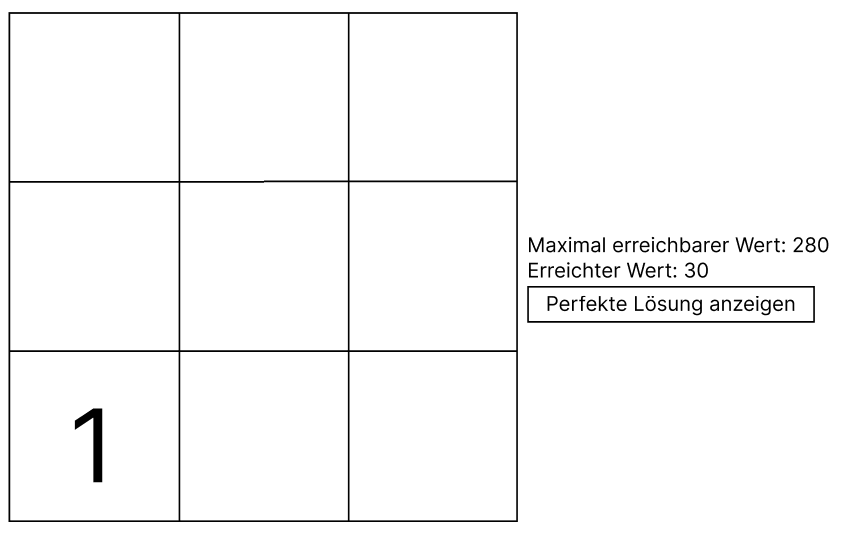
\includegraphics[scale=0.5]{images/itemAdded}
    \caption{Inventar mit erfolgreich hinzugefügtem Gegenstand}
    \label{fig:controller_itemAdded}
\end{figure}

Die Abbildung verdeutlicht die gelungene Integration des neuen Gegenstands in das Inventar. Durch eine klare visuelle
Darstellung signalisiert das \textit{Info Mesh} dem Benutzer unmissverständlich den aktualisierten Zustand des Inventars
und bestätigt die erfolgreiche Platzierung des Gegenstands.

Im Hintergrund wird das \texttt{usedItems}-Array aktualisiert, um den neuen Gegenstand zu integrieren:
\[
\text{usedItems} =
\left[
\begin{array}{ccccc}
0 & 0 & 0 \\
0 & 0 & 0 \\
1 & 0 & 0 \\
\end{array}
\right]
\]

Gleichzeitig wird der Gegenstand in das \texttt{processedItems}-Array aufgenommen, um sicherzustellen, dass er nicht
doppelt berücksichtigt wird:
\[
\text{processedItems} = \{1\}
\]

\subsubsection*{Gegenstand aus dem Inventar entfernt}
Dieser Zustand tritt ein, sobald der Benutzer einen Gegenstand aus dem Inventar entfernt hat, wie in Abbildung
\ref{fig:controller_itemRemoved} dargestellt.

%TODO: BILD VON ENTFERNTEM ITEM IN HOLOLENS MACHEN

\begin{figure}[H]
\centering
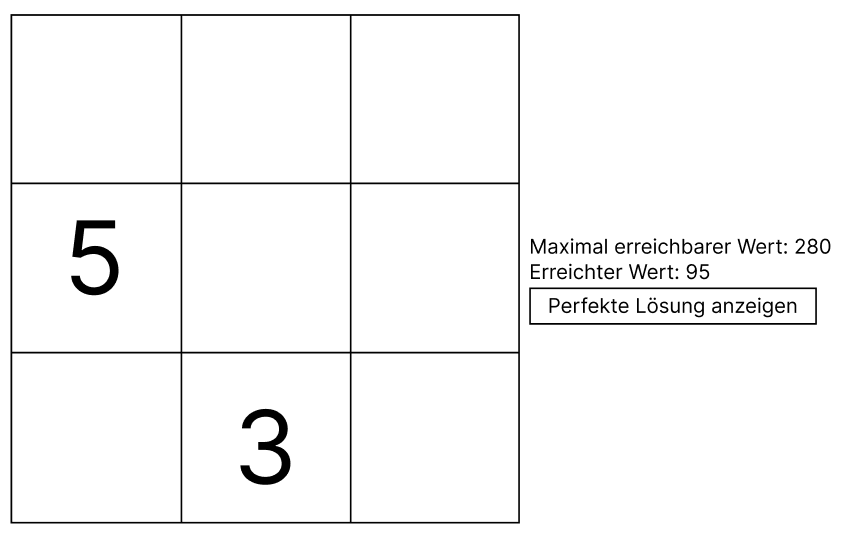
\includegraphics[scale=0.5]{images/itemEntfernt}
\caption{Inventar nach Entfernen eines Gegenstands}
\label{fig:controller_itemRemoved}
\end{figure}

Die Abbildung zeigt das Inventar nach Entfernen des Gegenstands aus der Position 4. Das \textit{Info Mesh} signalisiert
dem Benutzer deutlich den aktualisierten Zustand des Inventars und bestätigt die erfolgreiche Entfernung des Gegenstands.

Im Hintergrund wird das \texttt{usedItems}-Array aktualisiert, um den entfernten Gegenstand zu berücksichtigen:
\[
\text{usedItems(vorher)} =
\left[
\begin{array}{ccccc}
0 & 0 & 0 \\
5 & 1 & 0 \\
0 & 3 & 0 \\
\end{array}
\right]
\]

\[
\text{usedItems(nachher)} =
\left[
\begin{array}{ccccc}
0 & 0 & 0 \\
5 & 0 & 0 \\
0 & 3 & 0 \\
\end{array}
\right]
\]

Gleichzeitig wird der Gegenstand aus dem \texttt{processedItems}-Array entfernt, um sicherzustellen, dass er nicht
erneut verarbeitet wird:
\[
\text{processedItems (vorher)} = \{1\}
\]

\[
\text{processedItems (nachher)} = \{\}
\]

\subsubsection*{Gegenstand zu schwer für das Inventar}
Dieser Zustand tritt ein, wenn der Benutzer versucht, einen Gegenstand hinzuzufügen, der das Gewichtslimit des Inventars
überschreitet, wie in Abbildung \ref{fig:controller_itemTooHeavy} illustriert.

%TODO: BILD FÜR GEGENSTAND ZU SCHWER IN HOLOLENS MACHEN

\begin{figure}[H]
\centering
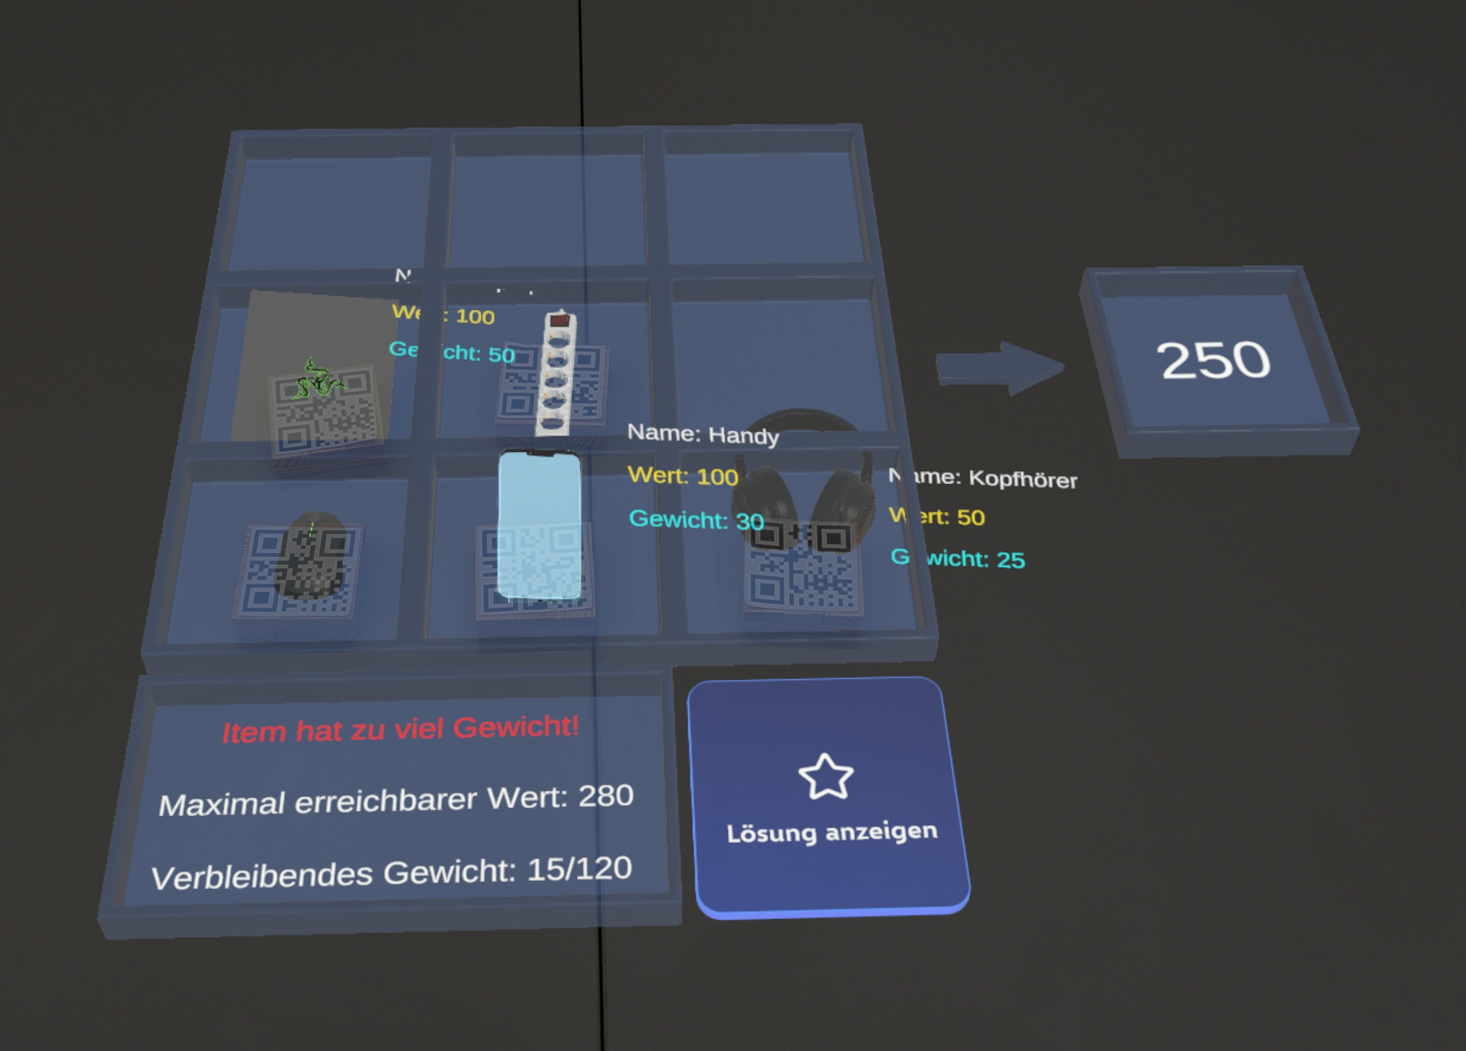
\includegraphics[scale=0.5]{images/itemToHeavy}
\caption{Inventar mit einem Gegenstand, der das Gewichtslimit überschreitet}
\label{fig:controller_itemTooHeavy}
\end{figure}

Die Abbildung zeigt das Inventar mit mehreren hinzugefügten Gegenständen. Die Reihenfolge in der diese Gegenstände
hinzugefügt wurden, ist die folgende: 1, 5, 3, 9. Dies ist wichtig, weil der zuletzt hinzugefügt Gegenstand den zu
schweren Gegenstand widerspiegelt. Auch zu sehen ist, dass das \textit{Info Mesh} den Benutzer deutlich über das
Überschreiten des Gewichtslimits informiert und das Hinzufügen des Gegenstands verhindert.

Im Hintergrund bleibt das \texttt{usedItems}-Array unverändert, da der Gegenstand nicht hinzugefügt wurde:
\[
\text{usedItems} =
\left[
\begin{array}{ccccc}
0 & 0 & 0 \\
5 & 0 & 0 \\
1 & 3 & 0 \\
\end{array}
\right]
\]
\\
Das \texttt{processedItems}-Array bleibt ebenfalls unverändert:
\[
\text{processedItems} = \{1, 5, 3\}
\]

\subsection{EventManager} \marginpar{\small\(\rightarrow\) HAYLAZ}

Der \textit{EventManager} ist ein entscheidendes Game-Objekt, das als zentrales Kommunikationselement fungiert und die
Interaktion zwischen verschiedenen Komponenten und Klassen innerhalb der Anwendung ermöglicht. Implementiert als Klasse
im Skript \textit{EventManager.cs}, das dem Game-Objekt angehängt ist, spielt er eine unverzichtbare Rolle trotz seiner
Kompaktheit, da er die Schnittstelle für die Kommunikation zwischen verschiedenen Klassen und Game-Objekten bereitstellt.

Das Konzept der Ereignisse ermöglicht die Kommunikation zwischen verschiedenen Teilen eines Programms, ohne dass direkte
Abhängigkeiten zwischen diesen Teilen bestehen müssen. Andere Teile des Codes können sich auf diese Ereignisse registrieren,
um benachrichtigt zu werden, wenn sie auftreten. In diesem Zusammenhang werden spezifische Ereignisse definiert:

\begin{itemize}
\item \textbf{Nachrichteneingang}: Dieses Event wird ausgelöst, wenn im ersten Level eine Nachricht von einem Laptop
empfangen wird. Nach dem Auslösen wird ein Ping-Paket über ein Kabel auf der Brille simuliert.
\item \textbf{Nachricht versendet}: Dieses Event wird ausgelöst, wenn im ersten Level eine Nachricht an einen Laptop
gesendet wird. Es dient dazu die Empfangene Nachricht an den zweiten Laptop im richtigen Moment (nach Abschluss der
Simulation) weiter zu leiten.
\item \textbf{Inventar Aktualisierung}: Dieses Event wird ausgelöst, wenn im zweiten Level ein Item ins Inventar gelegt und
das Inventar aktualisiert wird. Nach der Aktualisierung wird der aktuelle Wert des Inventars berechnet. Dadurch können
wir auf eine ständige Neuberechnung des Inventars verzichten und limitierte Ressourcen sparen.
\end{itemize}

Die Klasse \textit{EventManager} definiert diese Ereignisse als statische Ereignisse und stellt Methoden bereit, um die
Ereignisse auszulösen. Dies erleichtert die globale Verwendung des Ereignissystems in verschiedenen Teilen des Codes.
Die Aktionen (Actions) sind statisch, was bedeutet, dass sie auf Klassenebene definiert sind und keine Instanz der Klasse
benötigen, um aufgerufen zu werden. Die Methode \textit{Invoke} wird verwendet, um die Ereignisse auszulösen.

\begin{lstlisting}[style=csharp, label=code:EventManager]
public static class EventManager
{
// Szenario 1
// Ereignis für den Empfang einer Nachricht
public static event System.Action<int, string, string> OnMessageReceived;
// Methode zum Auslösen des Ereignisses für den Empfang einer Nachricht
public static void ReceiveMsg(int idx, string username, string message) => OnMessageReceived?.Invoke(idx, username, message);

// Ereignis für das Senden einer Nachricht
public static event System.Action<int, string, string> OnMessageSend;
// Methode zum Auslösen des Ereignisses für das Senden einer Nachricht
public static void SendMsg(int idx, string username, string message) => OnMessageSend?.Invoke(idx, username, message);

// Szenario 2
// Ereignis für die Aktualisierung des Inventars
public static event System.Action<int[,]> OnGridUpdate;
// Methode zum Auslösen des Ereignisses für die Aktualisierung des Inventars
public static void GridUpdate(int[,] grid) => OnGridUpdate?.Invoke(grid);
}
\end{lstlisting}

Der gezeigte Codeabschnitt definiert ein Ereignis und eine Methode, die verwendet werden, um auf die drei genannten Fälle zu reagieren. Durch die Definition des Ereignisses wird eine Möglichkeit geschaffen, dass andere Teile des Codes sich darauf registrieren können, um bei Auftreten des Ereignisses benachrichtigt zu werden.

Zum Beispiel wird in diesem Kontext das \textit{OnGridUpdate}-Ereignis definiert, um die Aktualisierung des Inventars zu signalisieren. Die Methode \textit{GridUpdate} dient dazu, dieses Ereignis auszulösen, indem sie es aufruft und dabei Informationen über das aktualisierte Inventar übergibt.

Um auf das aktualisierte Inventar zu reagieren, könnten andere Teile des Codes sich auf dieses Ereignis registrieren, indem sie eine Methode oder einen Handler bereitstellen, der ausgeführt wird, wenn das Ereignis eintritt, wie folgt:

\begin{lstlisting}[style=csharp label=code:Event Registration]
//Dieser Code Abschnitt befindet sich in der Klasse: KnapsackSolver.cs

void Start()
{
items = new QRItem(0).items;
// Die SetInventory Methode wird als Ereignishandler für das OnGridUpdate Ereignis registriert
EventManager.OnGridUpdate += SetInventory;
}

public void SetInventory(int[,] newInventory)
{
inventory = newInventory;
CalculateKnapsack();
}
\end{lstlisting}

Nachdem die Szene geladen wurde, registriert sich die Klasse \textit{KnapsackSolver} für das Ereignis \textit{OnGridUpdate}, indem sie die Methode \textit{SetInventory} als Ereignishandler verwendet. Das bedeutet, dass jedes Mal, wenn das Ereignis "OnGridUpdate" ausgelöst wird, die Methode \textit{SetInventory} aufgerufen wird, um den aktuellen Wert des neuen Inventars zu berechnen. Weiteres zur Berechnung des Inventarwertes ist in diesem Abschnitt zu finden, \ref{sec:MoritzInventarBerechnen}.


\begin{lstlisting}[style=csharp label=code:Event Trigger]
EventManager.GridUpdate(idGrid);
\end{lstlisting}

Das Auslösen des \textit{OnGridUpdate} Events wird durch den obigen Codeabschnitt erreicht. Dieser Codeabschnitt befindet
sich in der \textit{InventoryController} Klasse und wird aufgerufen, wenn ein neues Item hinzugefügt oder entfernt wird.

Insgesamt ermöglicht dieser simple Code eine lose Kopplung zwischen verschiedenen Teilen des Programms, indem Ereignisse verwendet
werden, um auf bestimmte Aktionen zu reagieren, ohne dass die beteiligten Teile voneinander wissen müssen. Dadurch wird die
Modularität, Erweiterbarkeit und Wartbarkeit der Anwendung gefördert.

\subsection{Das Knapsack Problem} \marginpar{\small\(\rightarrow\) {\tiny SKREPEK}}
Dieser Abschnitt befasst sich mit dem Knapsack-Problem, ein Kombinatorisches Optimierungsproblem. Dazu wird auch die
Problemstellung, welche Varianten und Typen des Problems es gibt, die zwei bekanntesten Algorithmen zum Lösen des Problems
und anschließend die Implementierung um zu das Problem zu lösen, erläutert.

\subsubsection{Problemstellung}
Das Knapsack-Problem befasst sich mit der Herausforderung, einen Rucksack optimal zu befüllen, unter der Ausnahme, dass
dieser eine begrenzte Kapazität aufweist. Um ihn zu füllen, steht eine Reihe von Gegenständen zu Auswahl, von denen jeder
einen individuellen Wert, der einen bestimmten Nutzen oder eine Wichtigkeit repräsentiert, hat. Jeder Gegenstand weißt
weiteres ein bestimmtes individuelles Gewicht, welches genau beschreibt, wie viel an Platz dieser Gegenstand im Rucksack
einnimmt, auf.

Das grundlegende Ziel beim Knapsack-Problem besteht darin, eine Auswahl von Gegenständen zu treffen, die in den Rucksack
passt und gleichzeitig den Gesamtwert der ausgewählten Gegenstände maximiert. Dabei darf die Summe der Gewichte der
ausgewählten Gegenstände die Kapazität des Rucksacks nicht überschreiten. Dies führt zu einer Herausforderung, bei der
eine perfekte Lösung gefunden werden muss, um den bestmöglichen Nutzen aus den verfügbaren Gegenständen zu ziehen.

\subsubsection{Typen des Knapsack-Problems}\label{sec:knapsackTypen}
Das Knapsack-Problem kann in verschiedene Typen unterteilt werden, die jeweils \textit{unterschiedliche Bedingungen}
und \textit{Anforderungen} haben. Nachfolgend werden die wichtigsten Typen des Knapsack-Problems erläutert.

%Quellen:
%https://www.geeksforgeeks.org/fractional-knapsack-problem/
%https://www.geeksforgeeks.org/0-1-knapsack-problem-dp-10/
%https://www.geeksforgeeks.org/extended-knapsack-problem/
%https://www.geeksforgeeks.org/unbounded-knapsack-repetition-items-allowed/
\subsubsection*{0/1 Knapsack-Problem}
Das 0/1-Knapsack-Problem bezieht sich auf die effiziente Auswahl von Gegenständen, um den maximalen Gesamtwert in einem
begrenzten Rucksack zu erreichen. Gegeben sind \textit{n} Gegenstand, wobei jedem Gegenstand ein bestimmtes Gewicht
(\textit{w}) und ein Wert (\textit{v}) zugeordnet ist. Außerdem steht ein Rucksack mit einer Kapazität (\textit{c}) zur
Verfügung. Das Ziel besteht darin, jene Gegenstände in den Rucksack zu legen, sodass die Summe der Werte der ausgewählten
Gegenstände maximal ist.

Es ist wichtig zu beachten, dass beim 0/1-Knapsack-Problem entweder ein Gegenstand \textit{vollständig} in den Rucksack
gepackt wird oder \textit{überhaupt nicht}. Es gibt keine Möglichkeit, einen Gegenstand \textit{teilweise} in den Rucksack
zu legen. Diese Beschränkung erfordert eine sorgfältige Auswahl der Gegenstände, um den verfügbaren Platz im Rucksack
optimal zu nutzen und gleichzeitig den Gesamtwert zu maximieren.\footnote{GeeksForGeeks, \cite{0/1 Knapsack-Problem}}

\subsubsection*{Fraktionales Knapsack-Problem}
Das fraktionale Knapsack-Problem befasst sich mit der effizienten Verteilung von Gegenständen in einem Rucksack, um den
Gesamtwert im Rucksack zu maximieren. Dabei werden die Gewichte und Werte von \textit{n} Gegenständen gegeben, und das
Ziel besteht darin, diese Gegenstände in einen Rucksack mit der \textit{Kapazität c} zu legen, um den maximalen Gesamtwert
zu erreichen. Im Gegensatz zum klassischen 0/1-Knapsack-Problem, bei dem entweder ein Gegenstand vollständig in den Rucksack
gepackt wird oder nicht, erlaubt das fraktionale Knapsack-Problem das Aufteilen von Gegenständen, z.B.: Das halbieren
eines Gegenstands, um den Gesamtwert im Rucksack zu maximieren. Diese Flexibilität ermöglicht es, eine perfekte Lösung
zu finden, indem die Gegenstände entsprechend ihrer Wertigkeit und Gewichtung effizient verteilt werden.\footnote{GeeksForGeeks, \cite{Fractional Knapsack Problem}}

\subsubsection*{Begrenztes Knapsack-Problem}
Das begrenzte Knapsack-Problem bezieht sich auf die effiziente Auswahl von Gegenständen, um den maximalen Gesamtwert
unter Berücksichtigung eines begrenzten Gewichts zu erreichen. Angenommen, es gibt \textit{n} Gegenstände, wobei jedem
Gegenstand ein bestimmtes Gewicht (\textit{w}) und ein Wert (\textit{v}) zugeordnet ist. Die Aufgabe besteht darin, den
Gesamtwert zu maximieren, indem von jedem gegebenen Gegenstand nur eine begrenzte Anzahl von Instanzen, deren Gesamtgewicht
nicht größer als das maximale Gewicht \textit{w} ist, verwendet werden darf.\footnote{GeeksForGeeks, \cite{Bounded Knapsack Problem}}

\subsubsection*{Unbegrenztes Knapsack-Problem}
Das unbeschränkte Knapsack-Problem befasst sich mit der effizienten Auswahl von Gegenständen, um den maximalen Gesamtwert
zu erreichen, wobei das Gesamtgewicht nicht größer als eine vorgegebene Kapazität ist. Angenommen, es gibt ein Rucksackgewicht
\textit{c} und eine Menge von \textit{n} Gegenständen, von denen jeder einen bestimmten Wert (\textit{v}) und ein
Gewicht (\textit{w}) hat. Das Ziel besteht darin, die maximale Menge zu berechnen, die genau dieses Gewicht erreichen kann.

Im Gegensatz zum Begrenzten Knapsack-Problem, bei dem die Anzahl der Instanzen eines Gegenstands begrenzt ist, können
beim unbeschränkten Knapsack-Problem \textit{beliebig viele} Instanzen \textit{desselben} Gegenstands verwendet werden.
Dies ermöglicht eine flexiblere Auswahl und Nutzung der verfügbaren Gegenstände, um den maximalen Gesamtwert zu erzielen,
der das vorgegebene Gewicht nicht überschreitet.\footnote{GeeksForGeeks, \cite{Unbounded Knapsack}}

\subsubsection{Variationen des Knapsack-Problems}
Im Laufe der Zeit hat das Knapsack-Problem verschiedene Variationen hervorgebracht, die jeweils unterschiedliche Aspekte
und Einschränken des Problems berücksichtigen. Variationen beziehen sich hier auf unterschiedliche Varianten des Hauptproblems,
also z.B. hat das 0/1 Knapsack-Problem verschiedene Varianten mit unterschiedlichen zusätzlichen Einschränkungen und
Aspekten. Nachfolgend werden die bekanntesten Variationen erläutert

%Quellen:
%https://en.wikipedia.org/wiki/Knapsack_problem#Multi-objective_knapsack_problem
%https://en.wikipedia.org/wiki/Knapsack_problem#Multi-dimensional_knapsack_problem
%https://en.wikipedia.org/wiki/Knapsack_problem#Multiple_knapsack_problem
%https://en.wikipedia.org/wiki/Knapsack_problem#Quadratic_knapsack_problem
%https://en.wikipedia.org/wiki/Knapsack_problem#Geometric_knapsack_problem
\subsubsection*{Mehrzieliges Knapsack-Problem}
Das mehrzielige Knapsack-Problem erweitert das klassische Knapsack-Problem, indem es mehrere \textit{Zielkriterien}
berücksichtigt. Anstatt nur den Gesamtwert der ausgewählten Gegenstände zu maximieren, sollen nun mehrere Ziele
\textit{gleichzeitig} optimiert werden. Zum Beispiel könnte neben der \textit{Maximierung} des Gesamtwerts auch die
\textit{Minimierung} des Gesamtgewichts oder anderer Kosten angestrebt werden. Diese Variation des Problems führt zu
komplexeren Optimierungsaufgaben, da Kompromisse zwischen den verschiedenen Zielen gefunden werden müssen.\footnote{Wikipedia, \cite{Multi-objective Knapsack-Problem}}

\subsubsection*{Multidimensionales Knapsack-Problem}
Beim multidimensionalen Knapsack-Problem hat jeder Gegenstand nicht nur ein Gewicht, sondern wird durch einen
\textit{m-dimensionalen} Vektor repräsentiert, der verschiedene \textit{Merkmale} oder \textit{Eigenschaften} des Gegenstands
darstellt. Entsprechend ist auch die Kapazität des Rucksacks ein \textit{m-dimensionaler} Vektor. Diese Variation des
Problems entsteht häufig in realen Anwendungen, in denen die Gegenstände durch mehrere Merkmale charakterisiert werden,
wie zum Beispiel \texit{Größe},\textit{Form}, \textit{Farbe} oder \textit{Material}.\footnote{Wikipedia, \cite{Multi-dimensional Knapsack-Problem}}

\subsubsection*{Mehrere Knapsack-Probleme}
Das multiple Knapsack-Problem \textit{erweitert} das klassische Knapsack-Problem, indem es \textit{mehrere} Rucksäcke
oder Behälter einführt, in die die Gegenstände verteilt werden können. Im Gegensatz zum klassischen Problem, bei dem
alle Gegenstände in einen einzelnen Rucksack gepackt werden müssen, können hier mehrere Rucksäcke genutzt werden, um die
Gegenstände aufzunehmen. Diese Variation ist relevant in Situationen, in denen die Gegenstände auf verschiedene Weise
organisiert oder verwendet werden sollen.\footnote{Wikipedia, \cite{Multi Knapsack-Problem}}

\subsubsection*{Quadratisches Knapsack-Problem}
Das quadratische Knapsack-Problem bezieht sich auf eine Variation, bei der das Ziel darin besteht, eine quadratische
Zielfunktion zu maximieren, die von den ausgewählten Gegenständen abhängt. Diese Zielfunktion kann beispielsweise den
Gesamtnutzen oder den Gesamtwert der ausgewählten Gegenstände darstellen und ist oft von quadratischer Form in Bezug auf
die Variablen, die die Auswahl der Gegenstände repräsentieren. Die Lösung dieses Problems erfordert spezielle Techniken
zur Bewältigung der quadratischen Struktur der Zielfunktion.\footnote{Wikipedia, \cite{Quadratic Knapsack-Problem}}

\subsubsection*{Geometrisches Knapsack-Problem}
Beim geometrischen Knapsack-Problem stehen eine Reihe von geometrischen Objekten mit unterschiedlichen \textit{Formen}
und \textit{Größen} zur Auswahl, die in einen \textit{rechteckigen Rucksack} gepackt werden sollen. Das Ziel besteht
darin, die Gegenstände so anzuordnen, dass der verfügbare Platz im Rucksack optimal genutzt wird und der Gesamtwert der
ausgewählten Gegenstände maximiert wird. Diese Variation des Knapsack-Problems erfordert eine \textit{Berücksichtigung}
der \textit{geometrischen Eigenschaften} der Objekte und kann in verschiedenen Anwendungen wie Layoutdesign oder
Packungsproblemen auftreten.\footnote{Wikipedia, \cite{Geometric Knapsack-Problem}}

%Quellen:
%https://www.hindawi.com/journals/mpe/2023/1742922/
\subsubsection{Ansätze zur Lösung des Knapsack-Problems}
Das Knapsack-Problem bietet Raum für eine Vielzahl von Lösungsansätzen, die sich in ihrer \textit{Komplexität},
\textit{Effizienz} und \textit{Genauigkeit} unterscheiden können. Diese Ansätze reichen von einfachen \textit{heuristischen}
Methoden bis hin zu \textit{komplexen optimierten} Algorithmen. Abgesehen von den bekanntesten Ansätzen wie den
\textit{dynamischen} und dem \textit{greedy} Ansatz, die später genauer betrachtet werden, gibt es weitere interessante
Möglichkeiten das Knapsack-Problem anzugehen.

Ein Ansatz besteht darin, das Problem in kleinere Teilprobleme zu zerlegen und diese dann unabhängig voneinander zu lösen.
Durch die Kombination der Lösungen dieser Teilprobleme kann eine Gesamtlösung gefunden werden. Diese Methode ist besonders
nützlich, wenn die Problemgröße groß ist und eine vollständige Suche nach einer optimalen Lösung zu aufwändig ist.

Eine weite Herangehensweise ist die Verwendung von \textit{Metaheuristiken}, wie etwa \textit{genetische Algorithmen}
oder \textit{Partikelschwarmoptimierung}. Die Algorithmen basieren auf biologischen oder sozialen Konzepten und verwenden
probabilistische Techniken, um Lösungen zu finden, die möglicherweise nicht optimal, aber dennoch akzeptable sind. Sie
eignen sich gut für komplexe Probleme, bei denen eine exakte Lösung schwer zu erreichen ist.\footnote{Hindawi, \cite{Solving the 0/1 Knapsack Problem Using Metaheuristic and Neural Networks}, S. 7 ff.}

Eine neuere Entwicklung in der Lösung des Knapsack-Problems ist der Einsatz von \textit{künstlicher Intelligenz}. Durch
den Einsatz von \textit{Datenanalyse} und \textit{statistischen Methoden} können Modelle trainiert werden, um Muster in
den Eigenschaften der Gegenstände und den Anforderungen des  Rucksacks zu erkennen und optimale Packstrategien vorherzusagen.

\subsubsection{Dynamischer Programmieransatz}
Der dynamische Programmieransatz ist eine leistungsfähige Methode zur Lösung des Knapsack-Problems, die auf der Idee beruht,
das Problem in kleinere Teilprobleme zu zerlegen und die Lösungen dieser Teilprobleme systematisch zu kombinieren, um die
optimale Gesamtlösung zu finden. Diese Methode eignet sich besonders gut für Probleme, bei denen Teilprobleme sich überlappen
und dieselben Teillösungen verwendet werden können, um mehrere Teilprobleme zu lösen.

Der folgende Pseudocode veranschaulicht den dynamischen Algorithmus zur Lösung des Knapsack-Problems:
\begin{lstlisting}[style=csharp, caption={Dynamischer Algorithmus}]
FUNCTION knapsackDynamic(weights[], values[], capacity)
    n = length(weights)
    DECLARE Tabelle[n + 1][capacity + 1]
    FOR i FROM 0 TO n DO
        FOR w FROM 0 TO capacity DO
            IF i == 0 OR w == 0 THEN
                Tabelle[i][w] = 0
            ELSE IF weights[i-1] <= w THEN
                Tabelle[i][w] = MAX(values[i-1] + Tabelle[i-1][w - weights[i-1]], Tabelle[i-1][w])
            ELSE
                Tabelle[i][w] = Tabelle[i-1][w]
            END IF
        END FOR
    END FOR
    RETURN Tabelle[n][capacity]
END FUNCTION
\end{lstlisting}\\
\\
Die Funktion \texttt{knapsackDynamic()} implementiert den dynamischen Programmieransatz zur Lösung des Knapsack-Problems.
Sie akzeptiert drei Parameter: ein Array von Gewichten (\( \textit{weights} \)), ein Array von Werten (\( \textit{values} \))
und die Kapazität des Rucksacks (\( \textit{capacity} \)).

Zuerst wird die Länge des Gewichtsarrays \( \textit{n} \) berechnet, um die Anzahl der verfügbaren Gegenstände zu bestimmen.
Dann wird eine Tabelle \( \textit{Tabelle} \) mit \( \textit{n+1} \) Zeilen und \( \textit{capacity+1} \) Spalten initialisiert.
Diese Tabelle dient dazu, die optimalen Werte für verschiedene Teilprobleme zu speichern.

Anschließend werden zwei verschachtelte Schleifen verwendet, um alle möglichen Kombinationen von Gegenständen und Gewichten
zu durchlaufen. Dabei wird für jedes Teilproblem in der Tabelle der optimale Wert berechnet. Die innere Schleife iteriert
über die möglichen Kapazitäten des Rucksacks, während die äußere Schleife die verfügbaren Gegenstände durchläuft.

Für jedes Teilproblem wird überprüft, ob der aktuelle Gegenstand in den Rucksack passt. Wenn ja, wird der Wert dieses
Gegenstands zu dem Wert addiert, der erreicht werden kann, wenn der Rucksack ohne diesen Gegenstand gefüllt wird. Andernfalls
wird der Wert aus der vorherigen Zeile der Tabelle übernommen, da der aktuelle Gegenstand nicht in den Rucksack passt.

Schließlich wird der Wert in der untersten rechten Zelle der Tabelle zurückgegeben, der den maximal erreichbaren Gesamtwert
des Rucksacks darstellt.

Dieser Algorithmus nutzt die Eigenschaften der optimalen Teilstruktur und des Überlappungsprinzips aus, um eine effiziente
Lösung des Knapsack-Problems zu finden. Durch die systematische Berechnung und Speicherung der optimalen Werte für Teilprobleme
ermöglicht der dynamische Programmieransatz eine Zeitkomplexität von \( O(n \cdot capacity) \), was für viele praktische
Anwendungen akzeptabel ist.

\subsubsection*{Aufbau und Interpretation der Tabelle der Teilprobleme}
Die Tabelle der Teilprobleme spielt eine entscheidende Rolle bei der systematischen Lösung des Knapsack-Problems mithilfe
des dynamischen Programmieransatzes. Sie ist eine zweidimensionale Matrix, die während des Algorithmusverlaufs generiert
wird und die optimalen Lösungen für verschiedene Teilprobleme des Knapsack-Problems enthält. Die Matrix ist wie folgt strukturiert:

\[
\text{dp = }
\left[
\begin{array}{ccccc}
a_{11} & a_{12} & a_{13} & \cdots & a_{1n} \\
a_{21} & a_{22} & a_{23} & \cdots & a_{2n} \\
a_{31} & a_{32} & a_{33} & \cdots & a_{3n} \\
a_{31} & a_{32} & a_{33} & \cdots & a_{3n} \\
\vdots & \vdots & \vdots & \ddots & \vdots \\
a_{m1} & a_{m2} & a_{m3} & \cdots & a_{mn} \\
\end{array}
\right]
\]

Jede \textit{Zeile} in der Matrix entspricht den verschiedenen verfügbaren Gewichtskapazitäten des Rucksacks, beginnend
bei \textit{null} und schrittweise bis zur \textit{maximalen Kapazität}.

Jede \textit{Spalte} in der Matrix repräsentiert die Anzahl der bereits \textit{berücksichtigten Gegenstände}, wobei jede
Spalte die \textit{Teilprobleme} für eine zunehmende Anzahl von Gegenständen darstellt.

Der letzte Eintrag in dieser Tabelle (\textbf{$\mathbf{a_{mn}}$}) repräsentiert den errechneten maximal erreichbaren Wert.\\
\\
Um anschließend eine Zelle \( a_{mn} \) dieser Matrix zu interpretieren und den maximalen erreichbaren Wert ablesen zu können, ist Folgendes wichtig:
\begin{enumerate}
\item \textbf{m} gibt an, wie viel \textit{Gewicht} bereits im Rucksack verbraucht wurde. Je weiter fortgeschritten dieser
Wert ist, daher desto weiter unten in der Tabelle, desto mehr Gewicht wurde bereits verwendet.
\item \textbf{n} gibt an, wie viele \textit{Gegenstände} bereits betrachtet wurden. Je weiter fortgeschritten, daher,
desto weiter rechts in der Tabelle, desto mehr Gegenstände wurden bereits berücksichtigt.
\end{enumerate}

Die Einträge in der Matrix werden durch den \textit{dynamischen Programmieransatz} berechnet, indem die optimalen Werte für
Teilprobleme \textit{schrittweise kombiniert} werden, um den Wert für größere Teilprobleme zu bestimmen.

\subsubsection*{Beispiel}
Angenommen, der Rucksack hat eine Kapazität von 5 und es sind die folgenden 5 Gegenstände (indiziert von 1 bis 5) mit den folgenden Werten und Gewichten gegeben:
\[
\begin{array}{|c|c|c|}
\hline
\text{Gegenstand} & \text{Wert} & \text{Gewicht} \\
\hline
1 & 10 & 5 \\
\hline
2 & 6 & 4 \\
\hline
3 & 8 & 3 \\
\hline
4 & 3 & 2 \\
\hline
5 & 7 & 1 \\
\hline
\end{array}
\]
\\
Auf der Grundlage dieser Informationen wird während des Durchlaufs des Knapsack-Algorithmus die Tabelle der Teilprobleme erzeugt, die wie folgt aussieht:

\[
\text{dp = }
\left[
\begin{array}{cccccc}
0 & 0 & 0 & 0 & 0 & 0 \\
0 & 0 & 0 & 0 & 0 & 10 \\
0 & 0 & 0 & 0 & 6 & 10 \\
0 & 0 & 0 & 8 & 8 & 10 \\
0 & 0 & 3 & 8 & 8 & 11 \\
0 & 7 & 7 & 10 & 15 & 15 \\
\end{array}
\right]
\]
\\
Auf der Grundlage dieser Tabelle kann der Schluss gezogen werden, dass der berechnete maximale Wert, der mit den gegebenen Objekten erreicht werden kann, 15 beträgt.

\subsubsection{Greedy-Ansatz}
Im Gegensatz zur dynamischen Lösung wählt der Greedy-Ansatz Gegenstände basierend auf bestimmten Kriterien aus, um eine
lokale Optimierung zu erreichen. Hierbei wird in jedem Schritt diejenige Entscheidung getroffen, die im Moment am
vorteilhaftesten erscheint, ohne jedoch die Gesamtoptimierung im Auge zu behalten.

Der folgende Pseudocode veranschaulicht den Greedy-Algorithmus zur Lösung des Knapsack-Problems:

\begin{lstlisting}[style=csharp, caption={Greedy Algorithmus}]
FUNCTION knapsackGreedy(weights[], values[], capacity)
    n = length(weights)
    DECLARE items[n]
    FOR i FROM 0 TO n DO
        items[i] = (values[i] / weights[i], weights[i], values[i])
    END FOR
    SORT items by ratio in descending order
    totalValue = 0
    currentWeight = 0
    FOR i FROM 0 TO n DO
        IF currentWeight + items[i].weight <= capacity THEN
            currentWeight += items[i].weight
            totalValue += items[i].value
        ELSE
            ratio = (capacity - currentWeight) / items[i].weight
            totalValue += ratio * items[i].value
            BREAK
        END IF
    END FOR
    RETURN totalValue
END FUNCTION
\end{lstlisting}\\
Die Funktion \texttt{knapsackGreedy()} nimmt wie der dynamische Ansatz drei Parameter an: ein Array von Gewichten (\( \textit{weights} \)),
ein Array von Werten (\( \textit{values} \)) und die Kapazität des Rucksacks (\( \textit{capacity} \)). Die Funktionsweise
dieses Ansatzes ist wie folgt:

\begin{enumerate}
\item Zunächst wird für jeden Gegenstand das Verhältnis von Wert zu Gewicht berechnet und in einer Liste von Tupeln
gespeichert. Jedes Tupel enthält das Wert-Gewichts-Verhältnis sowie das Gewicht und den Wert des entsprechenden Gegenstands.
\item Die Liste der Gegenstände wird basierend auf dem Verhältnis von Wert zu Gewicht in absteigender Reihenfolge
sortiert, um die Gegenstände mit dem höchsten Verhältnis zuerst zu betrachten.
\item Der Algorithmus durchläuft die sortierte Liste der Gegenstände und versucht, jeden Gegenstand dem Rucksack
hinzuzufügen. Dabei wird überprüft, ob das Hinzufügen des Gegenstands das Gewichtslimit des Rucksacks überschreitet.
Falls dies der Fall ist, wird ein Teil des Gegenstands entsprechend dem verbleibenden verfügbaren Gewicht im Rucksack hinzugefügt.
\item Nachdem alle Gegenstände überprüft wurden, wird der Gesamtwert der im Rucksack enthaltenen Gegenstände zurückgegeben.
Dies stellt die Lösung des Problems dar.
\end{enumerate}

Der Greedy-Algorithmus bietet eine einfache und effiziente Lösung für das Knapsack-Problem, die jedoch nicht immer die
perfekte Lösung garantiert. Durch die Auswahl der Gegenstände basierend auf lokalen Kriterien kann der Algorithmus zu
suboptimalen Ergebnissen führen, insbesondere wenn die Gegenstände stark voneinander abhängen oder das Gewichtslimit des
Rucksacks sehr restriktiv ist.

%Quellen:
%https://en.wikipedia.org/wiki/Knapsack_problem#Applications
\subsubsection{Anwendungen des Knapsack-Problems}
Die grundlegende Problemstellung des Knapsack-Problems hat breite Anwendung in verschiedenen \textit{wissenschaftlichen}
und \textit{industriellen} Bereichen gefunden, die sich mit der Allokation von Ressourcen beschäftigen, und bildet die
Grundlage für eine Vielzahl von Algorithmen und Anwendungen.

Dieses Kapitel untersucht die Anwendungen des Knapsack-Problems und seine Bedeutung in verschiedenen Domänen. Von der
\textit{Logistik} über die \textit{Finanzplanung} bis hin zum \textit{Ressourcenmanagement} hat das Knapsack-Problem
einen relevanten Einfluss auf die moderne Technologie und Wirtschaft.

Die Anwendungen des Knapsack-Problems lassen sich in folgende Hauptbereiche unterteilen:
\begin{enumerate}
\item \textbf{Logistik}: Der Knapsack-Algorithmus wird in der Logistik angewendet, um den Transport von Gütern mit
begrenzten Kapazitäten zu optimieren. Indem er die bestmögliche Auswahl von Gütern trifft, ermöglicht er Logistikunternehmen,
ihre Transportkosten zu minimieren und die Effizienz ihrer Lieferketten zu steigern. Dies kann die Beladung von Containern oder die Organisation von Waren in Lagern umfassen.
\item \textbf{Finanzplanung}: In der Finanzplanung wird der Knapsack-Algorithmus genutzt, um Portfolios von Investitionen
zu optimieren. Investoren können mithilfe dieses Algorithmus eine Auswahl von Wertpapieren treffen, die das Risiko
minimieren und den erwarteten Ertrag maximieren. Dies kann die Diversifizierung von Anlagen, die Auswahl von Aktien
oder die Verwaltung von Fonds umfassen.
\item \textbf{Ressourcenmanagement}: Der Knapsack-Algorithmus wird im Ressourcenmanagement verwendet, um die effiziente
Nutzung begrenzter Ressourcen sicherzustellen. Dies kann in der Produktion erfolgen, wo Arbeitskräfte, Maschinen und
Materialien effizient zugewiesen werden müssen, oder im Projektmanagement, um Zeit und Budgets zu optimieren. Durch
die Anwendung des Knapsack-Problems können Unternehmen ihre Produktivität steigern und Kosten senken.\footnote{Wikipedia, \cite{Knapsack-Problem Anwendungen}}
\end{enumerate}

Die Untersuchung dieser Anwendungen veranschaulicht die Vielseitigkeit und Effektivität des Knapsack-Problems bei der Lösung
komplexer Optimierungsprobleme. Darüber hinaus trägt die Anwendung des Knapsack-Algorithmus dazu bei, industrielle Abläufe
zu verbessern, Kosten zu senken und die Effizienz in verschiedenen Bereichen zu steigern.

\subsubsection{Auswahl des Implementierungsansatzes}
Die Wahl des Implementierungsansatzes für den Knapsack-Algorithmus für die in dieser Arbeit vorgestellten Anwendungen, ist von entscheidender Bedeutung
für den Erfolg des Projekts. Moderne Softwaresysteme stehen vor einer Vielzahl von Herausforderungen und Anforderungen,
die eine sorgfältige Auswahl eines geeigneten Algorithmus erforderlich machen.

Die Entscheidung für den Implementierungsansatz erfolgte nach einer eingehenden Analyse der Anforderungen der Anwendung
und einer gründlichen Untersuchung der verfügbaren Algorithmen sowie ihrer Eigenschaften. Dabei wurden verschiedene
Faktoren berücksichtigt, darunter die Notwendigkeit einer optimalen Lösung, die Effizienz der Algorithmusausführung, die
Flexibilität in Bezug auf unterschiedliche Problemvarianten und die Genauigkeit der berechneten Ergebnisse.

Diese Überlegungen werden anschließend ausführlich diskutiert und die Gründe für die Wahl des dynamischen Ansatzes als
Implementierungsstrategie für den Knapsack-Algorithmus erläutert:
\begin{enumerate}
\item \textbf{Perfekte Lösungsgarantie}: Der dynamische Ansatz bietet die Möglichkeit, eine perfekte Lösung für das
Knapsack-Problem zu garantieren. Dies ist besonders wichtig in Anwendungen, in denen eine genaue und zuverlässige
Lösung erforderlich ist, um optimale Entscheidungen zu treffen.
\item \textbf{Effizienz}: Obwohl der dynamische Ansatz im Vergleich zum Greedy-Ansatz einen höheren Rechenaufwand
erfordert, bietet er dennoch eine Laufzeit-effiziente Lösung für das Knapsack-Problem. Durch die Verwendung von dynamischer
Programmierung können Teilprobleme effizient gelöst und die Gesamtlösung optimiert werden.
\item \textbf{Flexibilität}: Der dynamische Ansatz ist flexibel und kann auf verschiedene Varianten des Knapsack-Problems
angewendet werden, einschließlich 0/1-Knapsack, unbeschränktem Knapsack und anderen Typen (siehe Abschnitt \ref{sec:knapsackTypen}). Dadurch ist er vielseitig
einsetzbar und kann an die spezifischen Anforderungen einer Anwendung angepasst werden.
\item \textbf{Genauigkeit}: Durch die Verwendung des dynamischen Ansatzes können exakte Werte für den maximal erreichbaren
Wert des Rucksacks und die optimale Auswahl von Gegenständen berechnet werden. Dies ermöglicht eine präzise Bewertung
und Planung basierend auf den berechneten Ergebnissen.
\end{enumerate}

In Anbetracht dieser Überlegungen wurde der dynamische Ansatz als die geeignete Methode zur Implementierung des Knapsack-Algorithmus
in dieser Anwendung gewählt. Obwohl nicht alle verfügbaren Lösungsansätze eine perfekte Lösung garantieren können, bieten
sie dennoch eine gute Balance zwischen Effizienz und Flexibilität. Aus diesem Grund erscheint der dynamische Ansatz als
ideale Wahl für die Behandlung des Knapsack-Problems in diesem Kontext, da er die Gewissheit einer optimalen Lösung bietet.

\subsubsection{Auswahl der Variante und Typ des Problems}
Die Wahl der Variante und des Typs des zu implementierenden Knapsack-Problems ist von entscheidender Bedeutung. Je nach
Variation und Typ ergeben sich unterschiedliche Aufgabenstellungen mit verschiedenen Bedingungen.

Nach einer gründlichen Analyse der Aufgabenstellung des Projekts wurde die endgültige Entscheidung für den Typ und die
zugehörige Variante getroffen. Dabei wurde festgestellt, dass das klassische Knapsack-Problem mit einer Kombination der
beiden Problem-Typen 0/1-Knapsack-Problem und Begrenztes-Knapsack-Problem die geeignete Wahl ist. Die Entscheidung für
den Typ 0/1 des Knapsack-Problems wurde getroffen, da die Aufgabenstellung des Anwendungsszenarios vorsieht, dass der
Benutzer Gegenstände in einem Inventar nur vollständig hinzufügen oder gar nicht hinzufügen kann. Und die Kombination
mit dem begrenzten Knapsack-Problem deswegen, weil in dieser Anwendung eine Begrenzung an Instanzen eines Gegenständen,
die dem Inventar hinzugefügt werden können, gesetzt ist.

\subsubsection{Der Knapsack Solver}
Das Unity Game Objekt \textit{Knapsack Solver}, wie in Abbildung \ref{fig:Knapsack_Editor} dargestellt, implementiert
die Lösung des Knapsack-Problems und berechnet gleichzeitig das zusammengestellte Inventar des Benutzers. Es stellt
Feedback über diese Berechnungen bereit. Dieses Game Objekt mit der angehängten Skript-Komponente \textit{Knapsack Solver}
implementiert die Klasse \textit{KnapsackSolver}, welche die Logik zur Berechnung des maximal erreichbaren Werts einer
optimalen Lösung sowie den Wert des selbst zusammengestellten Inventars steuert.

Die Klasse arbeitet eng mit der Klasse \textit{InventoryController} zusammen, um sicherzustellen, dass die Berechnungen
stets auf Grundlage des aktuellen individuell zusammengestellten Inventars des Benutzers erfolgen. Diese Interaktion
zwischen den beiden Klassen gewährleistet eine präzise und zeitnahe Verarbeitung der inventarbezogenen Informationen
innerhalb der Anwendung.

\begin{figure}[H]
    \centering
    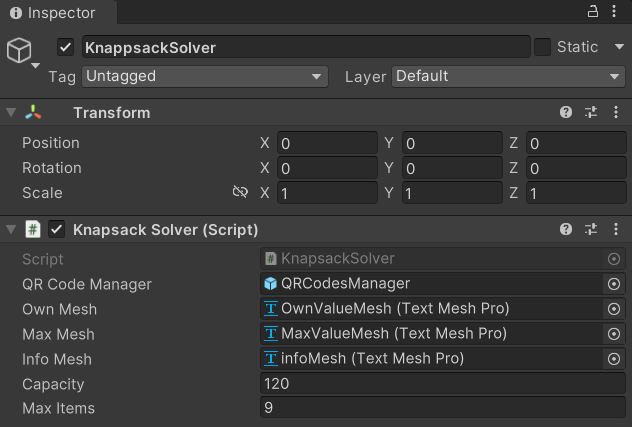
\includegraphics[scale=0.7]{images/knapsackEditor}
    \caption{KnapsackSolver Objekt im Editor}
    \label{fig:Knapsack_Editor}
\end{figure}

Abbildung \ref{fig:Knapsack_Editor} zeigt das Unity-Game-Objekt im Unity Inspektor. Ebenfalls dargestellt ist die angehängte
Skript-Komponente, die dem Game-Objekt zugeordnet ist. Innerhalb dieser Skript-Komponente sind die öffentlichen Klassenvariablen
aufgeführt, die direkt im Editor übergeben und manipuliert werden können. Diese Variablen spielen eine entscheidende Rolle
bei der Konfiguration und Steuerung des Knapsack Solvers. Zu den relevanten Variablen und ihrer Bedeutung gehören:
\begin{itemize}
    \item \textbf{QRCodesManager:} Ein Verweis auf das \textit{QRCodesManager} Game Objekt aus der Szene.

    \item \textbf{Own Mesh:} Referenz auf das \textit{OwnValueMesh} TextMesh-Element aus dem Inventar Prefab

    \item \textbf{Max Mesh:} Referenz auf das \textit{MaxValueMesh} TextMesh-Element aus dem Inventar Prefab

    \item \textbf{Info Mesh:} Referenz auf das \textit{infoMesh} TextMesh-Element aus dem Inventar Prefab

    \item \textbf{Capacity:} Integerwert, der die Kapazität des Rucksacks festlegt.

    \item \textbf{Max Items:} Integerwert, der die maximale Anzahl an möglich platzierbaren Gegenständen im Inventar
    festlegt.
\end{itemize}

\subsubsection{Knapsack-Algorithmus Implementierung}
Dieser Abschnitt behandelt die Implementierung der allgemeinen Variation des 0/1 Knapsack-Problems mittels des dynamischen
Programmieransatzes. Die Funktion \texttt{KnapsackMaxValue()} innerhalb der Klasse \textit{KnapsackSolver} implementiert
den Algorithmus und ermittelt eine perfekte Lösung, indem sie die verwendeten Gegenstände verfolgt, um den maximalen Wert
zu erreichen. Die Funktion besteht grundsätzlich aus zwei Hauptabschnitten, um dieses Ergebnis zu erzielen:
\begin{enumerate}
    \item \textbf{Algorithmus Implementation}: Zeilen 2 bis 23 aus Codeabschnitt \ref{code:startKnapsack} umfassen die
    Implementierung des Knapsack-Algorithmus.

    \item \textbf{Backtracking}: Zeilen 24 bis 42 aus Codeabschnitt \ref{code:startKnapsack} dienen dazu, das Array
    \texttt{usedItems} zu erstellen, welches eine perfekte Lösung repräsentiert.
\end{enumerate}

\begin{lstlisting}[style=csharp, caption={Knapsack Algorithmus / Item Backtracking}, label=code:startKnapsack]
public int KnapsackMaxValue(out int[,] usedItems) {
    int n = items.Count;
    int[,] dp = new int[n + 1, capacity + 1];
    bool[,] selected = new bool[n + 1, capacity + 1];
    for (int i = 0; i <= n; i++) {
        for (int w = 0; w <= capacity; w++) {
            if (i == 0 || w == 0)
                dp[i, w] = 0;
            else if (i <= maxItems && items[i].weight <= w) {
                int newValue = items[i].value + dp[i - 1, w - items[i].weight];
                if (newValue > dp[i - 1, w]) {
                    dp[i, w] = newValue;
                    selected[i, w] = true;
                } else {
                    dp[i, w] = dp[i - 1, w];
                    selected[i, w] = false;
                }
            } else {
                dp[i, w] = dp[i - 1, w];
                selected[i, w] = false;
            }
        }
    }
    int[,] tempUsedItems = new int[3, 3];
    int row = n;
    int col = capacity;
    int rowIndex = 0;
    int colIndex = 0;
    while (row > 0 && col > 0 && rowIndex < 3 && colIndex < 3) {
        if (selected[row, col] && colIndex < maxItems) {
            tempUsedItems[rowIndex, colIndex] = items[row].id;
            col -= items[row].weight;
            row--;
            colIndex++;
            if (colIndex >= 3) {
                colIndex = 0;
                rowIndex++;
            }
        } else {
            row--;
        }
    }
    usedItems = tempUsedItems;
    return dp[n, capacity];
}
\end{lstlisting}
Die vorliegende Implementierung des Lösungsansatzes für das Knapsack-Problem entspricht im Wesentlichen dem bereits
erklärten Pseudocode. Ein entscheidender Unterschied besteht jedoch darin, dass diese spezielle Implementierung eine
zusätzliche Bedingung berücksichtigt. Diese Bedingung besagt, dass bei der Berechnung des \textit{maximal} erreichbaren
Werts und der perfekten Lösung höchstens 9 Gegenstände aus den verfügbaren Gegenständen einbezogen werden dürfen. Diese
Einschränkung resultiert aus der Tatsache, dass der vorliegende Rucksack nur neun verfügbare Zellen hat, in denen ein
Gegenstand platziert werden kann.

Um diese Anforderung zu erfüllen, wird die zusätzliche Bedingung in die Implementierung integriert. Dies geschieht in
Zeile 9 des Codeabschnitts \ref{code:startKnapsack} durch folgende Bedingung:
\\
\begin{equation}
\begin{aligned}
i &\leq \text{maxItems} \land
\text{items}[i].\text{weight} &\leq w
\end{aligned}
\end{equation}

Während des Algorithmus wird zusätzlich ein Array aus booleschen Werten (\texttt{selected[][]}) erstellt, um die
ausgewählten Gegenstände für den maximalen Wert zu markieren. Dieses Array spielt eine wichtige Rolle im zweiten Abschnitt
der Funktion, um diese Gegenstände zurückzuverfolgen und die perfekte Lösung zusammenzustellen.

\subsubsection*{Aufbau und Interpretation der \textit{selected} Tabelle}
Angenommen, der Rucksack hat eine Kapazität von 5 und es sind die folgenden 5 Gegenstände (indiziert von 1 bis 5) mit den folgenden Werten und Gewichten gegeben:
\[
\begin{array}{|c|c|c|}
\hline
\text{Gegenstand} & \text{Wert} & \text{Gewicht} \\
\hline
1 & 10 & 5 \\
\hline
2 & 6 & 4 \\
\hline
3 & 8 & 3 \\
\hline
4 & 3 & 2 \\
\hline
5 & 7 & 1 \\
\hline
\end{array}
\]
\\
Aufgrund dieser Angaben wird die \texttt{selected} Matrix nach Ausführung des Knapsack-Algorithmus basierend auf den
ausgewählten Gegenständen gefüllt. Diese Matrix sieht dann folgendermaßen aus:

\[
\begin{array}{|c|c|c|c|c|c|}
\hline
& 0 & 1 & 2 & 3 & 4 \\
\hline
0 & \text{false} & \text{false} & \text{false} & \text{false} & \text{false} \\
\hline
1 & \text{false} & \text{false} & \text{false} & \text{false} & \text{true} \\
\hline
2 & \text{false} & \text{false} & \text{false} & \text{true} & \text{true} \\
\hline
3 & \text{false} & \text{false} & \text{true} & \text{true} & \text{true} \\
\hline
4 & \text{false} & \text{true} & \text{true} & \text{true} & \text{true} \\
\hline
5 & \text{false} & \text{true} & \text{true} & \text{true} & \text{true} \\
\hline
\end{array}
\]
Für die Interpretation der \texttt{selected}-Matrix ist es wichtig zu verstehen, wie sie funktioniert. Jede Zelle in dieser
Matrix gibt an, ob der entsprechende Gegenstand in der perfekten Lösung des Knapsack-Problems enthalten ist (\textit{true})
oder nicht (\textit{false}). Als Beispiel zeigt die Zelle $selected[4][3]$, dass der Gegenstand 4 in der perfekten Lösung
miteinbezogen wurde, als die Kapazität des Rucksacks 3 betrug. Diese Informationen ermöglichen folgende Schlussfolgerungen:
\begin{enumerate}
\item Der Index \textbf{i} in $selected[i][j]$ repräsentiert den Gegenstand, der in Betracht gezogen wird.
\item Der Index \textbf{j} in $selected[i][j]$ gibt die Kapazität des Rucksacks an, die für diese Teillösung verwendet
wurde.
\end{enumerate}

\subsubsection{Berechnung des zusammengestellten Rucksacks}
Um dem Benutzer ein dementsprechendes Feedback zu geben und dadurch zu veranschaulichen, welchen Wert der selbst
zusammengestellte Rucksack im Vergleich mit dem errechneten maximal erreichbaren Wert hat, wird hier eine Berechnung
benötigt, um diesen Wert zu berechnen. Diese Berechnung wird in der Funktion \texttt{KnapsackInventoryValue()} gehandhabt.
\begin{lstlisting}[style=csharp, caption={Funktion um eigenen Rucksack zu brechnen}]
public int KnapsackInventoryValue(int[,] inventory) {
    if (inventory == null) {
        throw new System.Exception("Inventory is null");
    }
    int totalValue = 0;
    foreach (var item in items.Values) {
        int itemId = item.id;
        int itemValue = item.value;
        for (int j = 0; j < inventory.GetLength(0); j++) {
            for (int k = 0; k < inventory.GetLength(1); k++) {
                if (inventory[j, k] == itemId) {
                    totalValue += itemValue;
                }
            }
        }
    }
    return totalValue;
}
\end{lstlisting}

Die Methode durchläuft mithilfe einer \texttt{foreach}-Schleife jeden Eintrag im Dictionary, welches alle vorhandenen
Gegenstände enthält. Dadurch kann auf die \texttt{ID} und den Wert (\texttt{Value}) jedes Gegenstands zugegriffen werden.
Anschließend iteriert die Methode durch das Array \texttt{usedItems}, welches eine perfekte Lösung repräsentiert, mittels
zweier \texttt{for}-Schleifen, um jeden Eintrag in diesem Array zu überprüfen. Dabei wird festgestellt, ob an der jeweiligen
Stelle \texttt{usedItems[i][j]} ein Wert gespeichert ist oder nicht. Falls das Array an der Indexposition \texttt{[i][j]}
der \texttt{ID} des aktuellen Gegenstands entspricht, wird der Wert dieses Gegenstands zum Gesamtwert (\texttt{totalValue})
addiert.

Nach Abschluss der Berechnung des zusammengestellten Rucksacks wird dieser Wert zurückgegeben, um ihn im weiteren Verlauf
der Applikation zu verwenden.

\subsection{Anzeigen der perfekten Lösung}\marginpar{\small\(\rightarrow\) {\tiny SKREPEK}}
Im Anwendungsszenario "Knapsack-Problem" ist das Anzeigen einer perfekten Lösung von entscheidender Bedeutung, da dies dem
Benutzer ermöglicht, eine perfekte Lösung zu visualisieren und zu verstehen, wie sie aussieht und welche Objekte sie enthält.

In diesem Abschnitt werden das Unity-Prefab \textit{Best Solution Prefab} und die zugehörige Skript-Komponente im Detail
beschrieben. Die Klasse \textit{BestSolutionVisualizer} ist hier hauptsächlich für das Platzieren, Aktivieren und Deaktivieren
der perfekten Lösung verantwortlich, um einen reibungslosen Ablauf zu gewährleisten. Es wird erklärt, wie das Prefab
selbst aufgebaut ist, wie dieses Skript aufgerufen wird und wie genau diese Lösung platziert und gefüllt wird.

\subsubsection{Aufbau und Hirarchie des best Solution Prefabs}
Das Design und die Struktur des Prefabs sind von entscheidender Bedeutung, da dieses Objekt als Grundlage für die
Visualisierung einer perfekten Lösung dient und dem Benutzer Feedback gibt. Die sorgfältige Ausarbeitung des Prefabs
trägt wesentlich zur Gesamterfahrung des Benutzers bei, erleichtert die Übersicht und fördert eine reibungslose Interaktion.
Das Prefab enthält nicht nur das einfache Inventar-Raster, sondern auch neun zusätzliche Elemente, die dem Inventar-Raster
untergeordnet sind und jeweils innerhalb einer Zelle platziert sind.
\begin{figure}[H]
    \centering
    \includegraphics[scale=0.3]{images/prefShow}
    \caption{Prefab Hirarchie und Aufbau im Unity Editor}
    \label{fig:InvPref}
\end{figure}
Die Abbildung \ref{fig:InvPref} stellt das gesamte Prefab im Unity Editor visuell dar und gibt gleichzeitig einen Einblick
in seine Hierarchie. Es wird deutlich, dass das Prefab aus einem Hauptmodell und neun Untermodellen besteht. Diese Modelle sind:
\begin{enumerate}
    \item \textbf{inventory}: Das Raster, welches den eigentlichen Rucksack repräsentiert.

    \item \textbf{QRItem}: Prefab, über das mithilfe der ID auf die 3D-Modelle zugegriffen wird, um diese darzustellen.
\end{enumerate}

\subsubsection{Das Best Solution Prefab}
Das Unity-Prefab \texttt{best Solution Prefab}, wie in Abbildung \ref{fig:bestSol_Editor} dargestellt, implementiert die
Logik zur Anzeige einer perfekten Lösung und gibt Feedback durch Visualisierung dieser Lösung. Dieses Prefab enthält die
angehängte Skript-Komponente \textit{Perfect Solution Visualizer}, die die Klasse \texttt{PerfectSolutionVisualizer}
implementiert. Diese Klasse ist für das Platzieren und Ausfüllen der perfekten Lösung verantwortlich.

\begin{figure}[H]
    \centering
    \includegraphics[scale=0.8]{images/bestSolPref_Editor}
    \caption{Game Objekt im Unity Editor}
    \label{fig:bestSol_Editor}
\end{figure}

Auf dieser Abbildung ist das \texttt{bestSolutionPrefab} Game Objekt mit den zugehörigen Komponenten in Unity selbst zu
sehen. An der Komponente, welches das Skript repräsentiert, ist zu sehen, dass dieses vier zu übergebende Objekte benötigt.
Darunter sind die folgenden:
\begin{itemize}
    \item \textbf{Perfect Solution Inventory:} Eine Referenz auf das \textit{Prefab} für die perfekte Lösung.
    \item \textbf{Inventory Placement Controller:} Eine Referenz auf das \texttt{inventoryPlacementController} Game Objekt.
    \item \textbf{Knapsack Solver:} Eine Referenz auf das \textit{Knapsack Solver} Game Objekt.
    \item \textbf{Inventory:} Eine Referenz auf das Raster Modell, dass im Best Solution Prefab enthalten ist.
\end{itemize}

Die korrekte Übergabe und Konfiguration dieser Objekte und Werte ist entscheidend für die Funktionalität dieser Klasse
und die tatsächliche Darstellung der perfekten Lösung.

\subsubsection{Auslöser des Skripts}
Die Anzeige der perfekten Lösung wird durch einen einfachen Knopfdruck ausgelöst, der sich innerhalb des \textit{Inventar Prefabs}
befindet. Wenn der Benutzer auf diesen Knopf drückt, wird das Skript zur Anzeige der perfekten Lösung gestartet. Dieses
Skript führt die notwendigen Funktionen und Operationen aus, um die perfekte Lösung zu visualisieren.

Die Abbilding \ref{fig:ScrAuf} zeigt die Verknüpfung des Scripts mit dem Knopf und verdeutlicht den Zusammenhang zwischen
dem Knopf im \texttt{Inventar Prefab} und dem Start des Skripts.

\begin{figure}[H]
    \centering
    \includegraphics[scale=0.8]{images/perfSolBut}
    \caption{Script Aufruf bei Knopfdruck}
    \label{fig:ScrAuf}
\end{figure}

In dieser Abbildung ist zu beachten, dass das interaktive Betätigen einer Schaltfläche durch die mitgelieferte Skript-Komponente
\textit{Pressable Button} ermöglicht wird. Diese Komponente stellt die Funktion \texttt{OnClicked()} bereit, die das
einfache Betätigen der Schaltfläche umsetzt. Diese Funktion löst dann die \texttt{Start()} Funktion der \texttt{bestSolutionVisualizer}
Klasse aus.

\subsubsection{Start des Perfect Solution Visualizer}
Nachdem der Benutzer den \texttt{Best Solution Button} betätigt hat, wird der entscheidende Prozess zur Anzeige der perfekten
Lösung gestartet. Dieser Prozess wird durch die Ausführung der Funktion \texttt{Start()} ausgelöst, wie im folgenden
Codeabschnitt \ref{code:Start_PSV} dargestellt.
\begin{lstlisting}[style=csharp, caption={PerfectSolutionVisualizer Start}, label=code:Start_PSV]
public void Start() {
    isClicked = !isClicked;
    if (isClicked == true) {
        anchorScript = inventoryPlacementObject.GetComponent<InventoryPlacementController>();
        originalInventoryPosition = anchorScript.objectPosition;
        knapsackSolver = KnapsackAlgoObject.GetComponent<KnapsackSolver>();
        perfectSolution = knapsackSolver.usedItems;
        setNewPosition();
        inventoryObject.SetActive(true);
        fillInventory();
    } else {
        inventoryObject.SetActive(false);
    }
}
\end{lstlisting}\\
Diese Funktion dient nicht nur als Auslöser für das Einblenden der Lösung, sondern auch für das Ausblenden der Lösung.
Eine zentrale Aufgabe besteht darin, sicherzustellen, dass der Benutzer die Lösung je nach Bedarf ein- oder ausblenden
kann. Um dies zu erzielen wird bei jedem Scriptaufruf die boolsche Variable \texttt{isClicked}, die den aktuellen Stand
der Sichtbarkeit des Modells repräsentiert, invertiert.

Abhängig von diesem boolschen Wert wird im weiteren Verlauf der Funktion entschieden, ob die perfekte Lösung sichtbar
werden soll (\texttt{true}) oder nicht (\texttt{false}). Um das Prefab dann anschließend an der korrekten Position platzieren
zu können wird auf die Positionsinformation des originalen platzierten Inventars-Prefabs (\texttt{objectPlaced}) zugegriffen
und ebenfalls wird auf das Array, welches die errechnete perfekte Lösung repräsentiert (\textt{usedItems}) zugegriffen
um das Prefab im weiteren Verlauf anhand dieser füllen zu können. Abschließend werden die beiden Funktion \texttt{setNewPosition()}
und \texttt{fillInventory()} aufgerufen die dies abschließen.

\subsubsection{Prefab der perfekten Lösung platzieren}
Die Platzierung des Prefabs der perfekten Lösung ist wichtig, um zu garantieren, dass es für den Benutzer leicht und
angenehm ist, diese zu sehen. Um dies zu garantieren, wird auf die Original-Position des Inventar-Objekts
(\texttt{originalInventoryPosition}) zugegriffen und aufgrund dessen eine neue Position errechnet. Um es für den Benutzer
jedoch angenehmer, d.h. besser für die allgemeine Benutzererfahrung, zu machen, die perfekte Lösung besser sehen zu
können, wird abschließend die Rotation dieses Objekts geändert, um es um -45 Grad entlang der x-Achse zu kippen.
\begin{lstlisting}[style=csharp, caption={Neue Position setzen}, label=code:newPos_PSV]
private void setNewPosition() {
    Vector3 newPosition = originalInventoryPosition + Vector3.forward * 0.395f + Vector3.up * 0.16f;
    inventoryObject.transform.position = newPosition;
    Quaternion objectRotation = Quaternion.Euler(-45f, 0f, 0f);
    inventoryObject.transform.rotation = objectRotation;
}
\end{lstlisting}\\

\subsubsection{Prefab füllen}
Aufgrund der Beschaffenheit des zuvor platzierten Objekts, das lediglich ein leeres Inventar-Objekt darstellt, ist es
notwendig, dieses im nächsten Schritt mit den passenden Elementen zu füllen oder die geeigneten Modelle zu aktivieren,
welche die perfekte Lösung repräsentieren. Diese Aufgabe wird durch den Aufruf der \texttt{fillInventory()} Funktion im
weiteren Verlauf des Skripts realisiert.
\begin{lstlisting}[style=csharp, caption={Inventar fuellen}, label=code:invFül_PSV]
private void fillInventory() {
    for (int i = 0; i < numRows; i++) {
        for (int j = 0; j < numColumns; j++) {
            int id = perfectSolution[i, j];
            if (perfectSolution[i, j] == 0)
                continue;
            else {
                string qrCodeName = "QRCode" + (i * numColumns + j + 1);
                Transform qrCodeTransform = inventory.Find(qrCodeName);
                if (qrCodeTransform != null) {
                    Transform childTransform = qrCodeTransform.Find(id.ToString());
                    if (childTransform != null) {
                        childTransform.gameObject.SetActive(true);
                    }
                }
            }
        }
    }
}
\end{lstlisting}\\
Diese Funktion \texttt{fillInventory()} durchläuft das zweidimensionale Array \texttt{perfectSolution}, das die perfekte
Lösung darstellt. Für jeden Eintrag wird geprüft, ob die ID des Elements ungleich \textit{Null} ist. Falls ja, wird ein
eindeutiger Bezeichner für das QRItem generiert und das entsprechende Unterelement des QRItems anhand der ID im Inventar
aktiviert. Ansonsten wird die Schleife übersprungen. Diese Funktion ermöglicht somit die Befüllung des Inventars mit den
entsprechenden Modellen gemäß der perfekten Lösung.

\subsubsection{Zustand nach Knopfdruck}
Nachdem der Benutzer den \texttt{Best Solution Button} betätigt hat und die entsprechende Skript-Komponente erfolgreich
ausgeführt wurde, wird die perfekte Lösung platziert und vervollständigt. Anschließend erhält der Benutzer eine Ansicht,
wie in Abbildung \ref{fig:perfSolUserPOV} dargestellt.
\begin{figure}[H]
    \centering
    \includegraphics[scale=0.8]{images/perfSolUserPOV}
    \caption{Perfekte Lösung}
    \label{fig:perfSolUserPOV}
\end{figure}


\section{Performance und Qualitätssicherung} \marginpar{\small\(\rightarrow\) HAYLAZ}

Die Sicherstellung einer hohen Performance und Qualität in Softwareprojekten ist entscheidend für den Erfolg und die Zufriedenheit der Nutzer. Ein zentraler Bestandteil dieser Bemühungen sind \textit{Unit-Tests}, die sicherstellen, dass einzelne Komponenten korrekt funktionieren und den Erwartungen entsprechen. Im Rahmen dieses Projekts wurden Unit-Tests zur Überprüfung des Knapsack-Algorithmus (\ref{sec:knapsackAlgorithmus}), der für das Projekt von entscheidender Bedeutung ist, genutzt. Die Verwendung des Unity Test Frameworks ermöglichte es, diese Tests effizient zu erstellen und auszuführen.

\subsection{\label{sec:testFramework}Unity Test Framework}

Das \textit{Unity Test Framework} stellt eine leistungsstarke Suite von Werkzeugen bereit, mit der Entwickler umfassende Tests für ihre Unity-Skripte schreiben und durchführen können. Von der Überprüfung von Variablen bis hin zur Validierung von erwarteten Ergebnissen bietet das Framework eine breite Palette von Funktionen, um die Qualität von Unity-Anwendungen zu gewährleisten.

\subsubsection{\label{sec:testRunner} Test-Runner}

Der \textit{Test-Runner} ist ein unverzichtbares Werkzeug innerhalb des \textit{Unity Test Frameworks}, das Entwicklern ermöglicht, Tests einfach zu organisieren, auszuführen und zu überwachen. Durch die intuitive Benutzeroberfläche können Testfälle gruppiert, in spezifischen Reihenfolgen ausgeführt und detaillierte Berichte über den Testdurchlauf generiert werden. Die visuelle Darstellung in Abbildung \ref{fig:testRunner} bietet einen schnellen Überblick über die Testergebnisse und ermöglicht eine präzise Analyse der Codequalität.

In der Abbildung \ref{fig:testRunner} ist der \textit{Test-Runner} dargestellt. Dort sind auch die implementierten Tests dieses Projekts ersichtlich, insgesamt vier Tests mit mehreren TestCases. Weitere Details dazu finden sich im Abschnitt \ref{sec:tests}.

\begin{figure}[H]
\centering
\includegraphics[scale=0.04, angle=0]{images/testRunner}
\caption{Test-Runnner Fenster}
\label{fig:testRunner}
\end{figure}

\subsubsection{\label{sec:AAA} AAA-Schema}
Das AAA-Schema steht für "Arrange, Act, Assert" und ist ein grundlegendes Konzept im Bereich des Testens von Software. Es bietet eine klare Struktur für die Organisation von Testfällen, um sicherzustellen, dass die Funktionalität korrekt überprüft wird. Hier ist eine Erläuterung der einzelnen Schritte:
\begin{itemize}
    \item \textbf{Arrange (Vorbereitung):} In diesem Schritt werden die Vorbedingungen für den Testfall eingerichtet.
Dies beinhaltet die Initialisierung von Objekten, das Setzen von Parametern und das Festlegen des Kontexts, um sicherzustellen, dass die zu testende Funktionalität in einem definierten Zustand ausgeführt wird.
Das Ziel ist es, eine klare Umgebung für den Test zu schaffen, damit die zu überprüfende Funktionalität isoliert und unabhängig getestet werden kann.
    \item \textbf{Act (Ausführung):}
Hier wird die tatsächliche Aktion oder Methode aufgerufen, die getestet werden soll.
Dies kann das Aufrufen einer Methode, das Ausführen einer Funktion oder das Durchführen einer bestimmten Aktion sein, die das zu testende Verhalten auslöst.
Das Ziel ist es, die spezifische Funktionalität auszuführen, die überprüft werden soll, um festzustellen, ob sie das erwartete Verhalten aufweist.
    \item \textbf{Assert (Überprüfung):}

In diesem Schritt wird das erwartete Verhalten mit dem tatsächlichen Ergebnis verglichen.
Es wird überprüft, ob das Ergebnis der ausgeführten Aktion den Erwartungen entspricht.
Wenn das Ergebnis den Erwartungen entspricht, gilt der Testfall als bestanden. Andernfalls wird der Testfall als fehlgeschlagen markiert und eine entsprechende Fehlermeldung ausgegeben.
Das Ziel ist es, sicherzustellen, dass die Funktionalität wie erwartet funktioniert und potenzielle Fehler oder Abweichungen identifiziert werden.
\end{itemize}

Das AAA-Schema trägt zur Verbesserung der Lesbarkeit, Wartbarkeit und Strukturierung von Testfällen bei, indem es eine klare Trennung der einzelnen Schritte ermöglicht. Dadurch wird die Testentwicklung effizienter und erleichtert die Identifizierung und Behebung von Fehlern.

%TODO: Quelle https://automationpanda.com/2020/07/07/arrange-act-assert-a-pattern-for-writing-good-tests/
\subsection{Testfälle}

Dieser Abschnitt bietet eine detaillierte Beschreibung der durchgeführten Tests. Alle einzelnen Testfälle sind innerhalb der Klasse \textit{KnapsackSolverTests} (\ref{code:testClass}) organisiert. Die Test-Klasse fungiert als eine Sammlung von Methoden, die verschiedene Aspekte einer spezifischen Funktionalität überprüfen, nämlich den \textit{Knapsack Algorithmus}.

\begin{lstlisting}[style=csharp, caption={Auszug aus der Test-Klasse}, label={code:testClass}]
[TestFixture]
public class KnapsackSolverTests
{
    // Eine Variable zur Speicherung der KnapsackSolver-Instanz
    private KnapsackSolver knapsackSolver;

    // Die SetUp-Methode wird vor jedem Testfall ausgeführt
    [SetUp]
    public void SetUp()
    {
        // Erstellen eines GameObjects für den KnapsackSolver
        GameObject solverObject = new GameObject("KnapsackSolverObject");

        // Dem GameObject wird eine Instanz von KnapsackSolver hinzugefügt
        knapsackSolver = solverObject.AddComponent<KnapsackSolver>();
    }

    // Hier folgen die einzelnen Testfälle...
}
\end{lstlisting}

Wie ersichtlich ist, werden verschiedene Attribute verwendet, die vom Unity Test Framework (\ref{sec:testFramework}) bereitgestellt werden. Diese Attribute haben bestimmte Zwecke und Funktionalitäten innerhalb des Testframeworks. Das \textit{TestFixture-Attribut} kennzeichnet die Klasse \textit{KnapsackSolverTests} als Testfixture, was dem Framework signalisiert, dass die Klasse Tests enthält, die ausgeführt werden sollen. Das \textit{SetUp-Attribut} bewirkt, dass vor jedem Test die Methode \textit{SetUp()} ausgeführt wird. Der Inhalt der SetUp-Methode stellt sicher, dass stets eine neue Instanz des \textit{KnapsackSolvers} (\ref{sec:moKnapsacksolver}) erstellt wird, wodurch die Funktionalität der Tests immer in einer sauberen Ausgangssituation getestet werden kann.

Diese Struktur gewährleistet eine konsistente Umgebung vor jedem Testfall und ermöglicht es, dass die Tests isoliert und unabhängig voneinander ausgeführt werden können.


\subsubsection{Aufbau eines einzelnen Testfalls}

\begin{lstlisting}[style=csharp, caption={einzelner Testfall}, label={code:zeroTest}]
    [Test]
    public void KnapsackMaxValue_NoItems_ReturnsZero()
    {
        // Arrange
        knapsackSolver.items = new Dictionary<int, QRData>();
        knapsackSolver.capacity = 100;

        // Act
        int maxValue = knapsackSolver.KnapsackMaxValue(out int[,] usedItems);

        // Assert
        Assert.AreEqual(0, maxValue, "The maximum value should be zero when there are no items.");
    }
\end{lstlisting}

Um sicherzustellen, dass die Funktionalität korrekt überprüft wird, folgt ein Testfall im Unity Test Framework einem spezifischen Aufbau. Im obigen Beispiel (Code \ref{code:zeroTest}) wird ein Testfall dargestellt, der sicherstellt, dass der maximale Wert des Rucksacks korrekt berechnet wird, wenn keine Gegenstände im Rucksack vorhanden sind. Dieser Testfall gliedert sich in drei Hauptteile, die nach dem sogenannten \textit{AAA-Schema}(\ref{sec:AAA}) strukturiert sind.

Im Vorbereitungsabschnitt (\textit{Arrange}) werden die erforderlichen Vorbedingungen für den Testfall eingerichtet. In diesem Fall werden dem KnapsackSolver keine Gegenstände hinzugefügt, und die Kapazität des Rucksacks wird auf 100 gesetzt.

Im Ausführungsabschnitt (\textit{Act}) wird die tatsächliche Methode oder Funktionalität aufgerufen, die getestet werden soll. Hier wird die Methode \texttt{KnapsackMaxValue} des KnapsackSolver-Objekts aufgerufen, um den maximalen Wert des Rucksacks zu berechnen.

Im Überprüfungsabschnitt (\textit{Assert}) wird das erwartete Ergebnis mit dem tatsächlich berechneten Ergebnis verglichen. In diesem Fall wird überprüft, ob der maximal berechnete Wert tatsächlich null ist, da keine Gegenstände im Rucksack vorhanden sind. Wenn der Test fehlschlägt, wird eine entsprechende Fehlermeldung ausgegeben.

Durch die Strukturierung von Testfällen nach dem \textit{AAA-Schema} wird eine klare und strukturierte Organisation erreicht. Dies verbessert die Lesbarkeit und Wartbarkeit des Testcodes erheblich und erleichtert die Identifizierung und Behebung von Fehlern.

\subsubsection{Testen von Einzelgegenständen im Rucksack}

\begin{lstlisting}[style=csharp, caption={Testfall: einzelne Gegenstände}, label={code:einzelTest}]
    [TestCase(20, 50, 30, ExpectedResult = 50,
    TestName = "Single item within capacity returns expected value.")]
    [TestCase(30, 50, 20, ExpectedResult = 0,
    TestName = "Single item exceeding capacity returns zero value.")]
    [TestCase(30, 50, 30, ExpectedResult = 50,
    TestName = "Single item exact capacity returns expected value.")]
    public int KnapsackMaxValue_SingleItem_ReturnsExpectedValue(
    int weight, int value, int capacity)
    {
        // Arrange
        var item = new QRData { id = 1, weight = weight, value = value };
        knapsackSolver.items = new Dictionary<int, QRData> { { 1, item } };
        knapsackSolver.capacity = capacity;

        // Act
        return knapsackSolver.KnapsackMaxValue(out _);
    }
\end{lstlisting}

Die oben aufgeführten Testfälle zeigen verschiedene Szenarien zur Berechnung des maximalen Werts eines Rucksacks mit nur einem Gegenstand. Jeder Testfall wird mittels des \texttt{[TestCase]}-Attributs definiert und enthält das Gewicht, den Wert und die Kapazität des Rucksacks als Parameter. Das erwartete Ergebnis wird ebenfalls angegeben, um sicherzustellen, dass die berechneten Werte den Erwartungen entsprechen. Im Vorbereitungsabschnitt werden die notwendigen Vorbedingungen festgelegt, indem ein einzelner Gegenstand mit den angegebenen Gewicht und Wert dem KnapsackSolver hinzugefügt wird. Die Kapazität des Rucksacks wird entsprechend gesetzt. Im Ausführungsabschnitt wird die Methode \texttt{KnapsackMaxValue} aufgerufen, um den maximalen Wert des Rucksacks zu berechnen. Das zurückgegebene Ergebnis wird überprüft und mit dem erwarteten Ergebnis verglichen. Durch diese Testfälle wird sichergestellt, dass die Methode zur Berechnung des maximalen Werts unter verschiedenen Bedingungen korrekt arbeitet.

Im zweiten Testfall wird die Methode \texttt{KnapsackMaxValue\_SingleItem\_ReturnsExpectedValue} verwendet, die mit dem \texttt{[TestCase]}-Attribut versehen ist, um verschiedene Szenarien für die Berechnung des maximalen Werts eines Rucksacks mit nur einem Gegenstand zu testen. Im Gegensatz zum ersten Testfall (\ref{code:zeroTest}), der die \texttt{[Test]}-Annotation verwendet, um einen einzelnen Testfall zu definieren, wird hier die \texttt{[TestCase]}-Annotation verwendet, um mehrere Testfälle innerhalb derselben Methode zu definieren.

Die Verwendung von \texttt{[TestCase]} ermöglicht eine kompaktere Darstellung mehrerer ähnlicher Testfälle, wodurch der Code übersichtlicher wird. Jeder Testfall wird durch die Parameter definiert, die an die Methode übergeben werden, und das erwartete Ergebnis wird durch das \texttt{ExpectedResult}-Attribut angegeben. Das \textit{TestName}-Attribut trägt auch der Übersichtlichkeit und der Lesbarkeit bei. Dieser Name wird dann auch im \textit{Test-Runner} (\ref{sec:testRunner}) angezeigt, mit dem entsprechenden Bericht zum TestCase.

\subsubsection{Testen von mehreren Gegenständen im Rucksack}

\begin{lstlisting}[style=csharp, caption={Testfall: mehrere Gegenstände}, label={code:mehrTest}]
    [TestCase(10, ExpectedResult = 0,
    TestName = "All items exceeding capacity return zero value.")]
    [TestCase(90, ExpectedResult = 220,
    TestName = "All items within capacity return expected value.")]
    [TestCase(70, ExpectedResult = 170,
    TestName = "Multiple items within capacity, return optimal selection.")]
    public int KnapsackMaxValue_MultipleItems_ReturnsExpectedValue(
    int capacity)
    {
        // Arrange
        var items = new Dictionary<int, QRData>
        {
            { 1, new QRData { id = 1, weight = 20, value = 50 } },
            { 2, new QRData { id = 2, weight = 30, value = 70 } },
            { 3, new QRData { id = 3, weight = 40, value = 100 } }
        };
        knapsackSolver.items = items;
        knapsackSolver.capacity = capacity;

        // Act
        return knapsackSolver.KnapsackMaxValue(out _);
    }
\end{lstlisting}

Dieser Codeabschnitt demonstriert Testfälle für die Berechnung des maximalen Werts eines Rucksacks, wenn mehrere Gegenstände hinzugefügt werden. Ähnlich wie im vorherigen Abschnitt werden auch hier die Testfälle mit dem \texttt{[TestCase]}-Attribut definiert, wobei jedes Testcase nur die Kapazität des Rucksacks als Parameter hat und das erwartete Ergebnis angibt.

Im Vorbereitungsabschnitt (\textit{Arrange}) werden die notwendigen Vorbedingungen festgelegt, indem eine Sammlung von Gegenständen erstellt wird. Jeder Gegenstand wird durch ein \texttt{QRData}-Objekt repräsentiert, das Gewicht und Wert enthält. Diese Gegenstände werden dann dem \texttt{knapsackSolver} hinzugefügt, und die Kapazität des Rucksacks wird entsprechend gesetzt.

Im Ausführungsabschnitt (\textit{Act}) wird die Methode \texttt{KnapsackMaxValue} aufgerufen, um den maximalen Wert des Rucksacks zu berechnen. Das zurückgegebene Ergebnis wird dann überprüft und mit dem erwarteten Ergebnis verglichen.

\subsubsection{Performance-Messung}

\begin{lstlisting}[style=csharp, caption={Codeabschnitt: Performance Messung bei hoher Anzahl an Gegenständen}, label={code:performanceRange}]
    [Test]
    public void KnapsackPerformanceReportItemRange()()
    {
        // Überschrift für den Leistungsbericht ausgeben
        UnityEngine.Debug.Log("Item Count | Elapsed Time (ms)");
        UnityEngine.Debug.Log("-----------------------------");

        // Schleife durch verschiedene Gegenstandanzahlen
        for (int itemCount = 50; itemCount <= 1000; itemCount += 50)
        {
            // Oberen Grenzwert für das Gegenstandgewicht und die Kapazität basierend auf der Gegenstandanzahl berechnen
            int weightUpperBound = itemCount * 2;
            int capacity = itemCount * 5;

            // Zufällige Gegenstände generieren
            var items = GenerateRandomItems(itemCount, weightUpperBound);

            // Gegenstände und Kapazität für den Rucksacklöser festlegen
            knapsackSolver.items = items;
            knapsackSolver.capacity = capacity;

            // Stoppuhr starten, um die verstrichene Zeit zu messen
            var stopwatch = Stopwatch.StartNew();

            // Die zu testende Methode aufrufen
            knapsackSolver.KnapsackMaxValue(out _);

            // Stoppuhr anhalten nach dem Methodenaufruf
            stopwatch.Stop();

            // Anzahl der Gegenstände und verstrichene Zeit für diese Iteration ausgeben
            UnityEngine.Debug.Log($"{itemCount,-10} | {stopwatch.ElapsedMilliseconds,-15}");
        }
    }
\end{lstlisting}

Der vorliegende Codeabschnitt implementiert eine Testmethode namens \textit{KnapsackPerformanceReport}, die darauf abzielt, die Leistung des Knapsack Algorithmus unter verschiedenen Lastszenarien zu bewerten. Der Code ist auf die Performance-Messung des Algorithmus fokussiert und zielt darauf ab, die Laufzeit des Algorithmus in Abhängigkeit von der Anzahl der Gegenstände im Rucksack zu erfassen.

Die Methode beginnt mit der Ausgabe einer Überschrift, die das Format des folgenden Leistungsberichts festlegt. Im Hauptteil der Methode wird eine Schleife durchlaufen, die verschiedene Anzahlen von Gegenständen im Rucksack simuliert. Die Anzahl der Gegenstände steigt schrittweise von 50 bis 1000, wobei in jedem Schritt 50 Gegenstände hinzugefügt werden. Innerhalb der Schleife werden zunächst der obere Grenzwert für das Gewicht der Gegenstände und die Kapazität des Rucksacks basierend auf der aktuellen Anzahl von Gegenständen berechnet. Anschließend werden zufällige Gegenstände generiert, die in den Rucksack aufgenommen werden sollen. Die generierten Gegenstände sowie die Kapazität des Rucksacks werden dann dem Algorithmus zugewiesen.
Um die Leistung des Algorithmus zu messen, wird für jede Iteration der Schleife eine Stoppuhr gestartet, bevor die Methode "KnapsackMaxValue" aufgerufen wird, um den maximalen Wert des Rucksacks zu berechnen. Nach Beendigung des Methodenaufrufs wird die Stoppuhr gestoppt, und die verstrichene Zeit wird zusammen mit der Anzahl der Gegenstände im Rucksack protokolliert.


\begin{lstlisting}[style=csharp, caption={Codeabschnitt: Performance Messung bei 500 Aufrufen von 20 Gegenständen}, label={code:performanceIteration}]
    [Test]
    public void KnapsackPerformanceReportRangeIteration()
    {
        // Überschrift für den Leistungsbericht ausgeben
        UnityEngine.Debug.Log("Iteration | Elapsed Time (ms)");
        UnityEngine.Debug.Log("-----------------------------");

        // Konstante für die Anzahl der Gegenstände
        int itemCount = 20;

        // Oberen Grenzwert für das Gegenstandgewicht basierend auf der Gegenstandanzahl berechnen
        int weightUpperBound = itemCount * 2;

        // Schleife für 1000 Mal wiederholen
        for (int i = 1; i <= 500; i++)
        {
            // Oberen Grenzwert für die Kapazität basierend auf der Gegenstandanzahl berechnen
            int capacity = itemCount * 5;

            // Zufällige Gegenstände generieren (festgelegte Anzahl von Gegenständen)
            var items = GenerateRandomItems(itemCount, weightUpperBound);

            // Gegenstände und Kapazität für den Rucksacklöser festlegen
            knapsackSolver.items = items;
            knapsackSolver.capacity = capacity;

            // Stoppuhr starten, um die verstrichene Zeit zu messen
            var stopwatch = Stopwatch.StartNew();

            // Die zu testende Methode aufrufen
            knapsackSolver.KnapsackMaxValue(out _);

            // Stoppuhr anhalten nach dem Methodenaufruf
            stopwatch.Stop();

            // Durchlaufnummer und verstrichene Zeit für diese Iteration ausgeben
            UnityEngine.Debug.Log($"{i,-9} | {stopwatch.ElapsedTicks / (Stopwatch.Frequency / (1000.0 * 1000.0)):F2} µs");
        }
    }
\end{lstlisting}


Dieser Codeabschnitt \textit{KnapsackPerformanceReportRangeIteration} (\ref{code:performanceIteration}) unterscheidet sich vom anderen Codeabschnitt \textit{KnapsackPerformanceReportItemRange} (\ref{code:performanceRange}) hauptsächlich in Bezug auf die Parameter, die für die Leistungsmessung verwendet werden.

Im Abschnitt KnapsackPerformanceReportRangeIteration wird die Leistung des Knapsack-Algorithmus bei einer festen Anzahl von 20 Gegenständen und 500 Durchläufen gemessen. Dies bedeutet, dass die Anzahl der Gegenstände konstant bleibt, während die Iterationen variiert werden, um die Konsistenz der Messung sicherzustellen und die Auswirkungen wiederholter Durchläufe zu beobachten. Im Gegensatz dazu bewertet der Abschnitt KnapsackPerformanceReportItemRange die Leistung des Algorithmus bei einer variablen Anzahl von Gegenständen, wobei die Anzahl der Gegenstände von 50 bis 1000 in Schritten von jeweils 50 erhöht wird. Dies ermöglicht die Untersuchung der Leistung des Algorithmus bei verschiedenen Lastszenarien und die Identifizierung möglicher Zusammenhänge zwischen der Anzahl der Gegenstände und der Ausführungszeit des Algorithmus.

Darüber hinaus verwendet der Abschnitt KnapsackPerformanceReportItemRange eine andere Methode zur Messung der verstrichenen Zeit, indem die Methode ElapsedMilliseconds der Stopwatch-Klasse verwendet wird, um die Zeit in Millisekunden zu erfassen. Im Gegensatz dazu verwendet der Abschnitt KnapsackPerformanceReportRangeIteration die Berechnung der verstrichenen Ticks und deren Umrechnung in Mikrosekunden für eine genauere Messung.

%TODO: Excel ss einbauen

Basierend auf den Performance-Messungen können folgende Schlussfolgerungen gezogen werden:
\begin{itemize}
    \item \textbf{Laufzeitverhalten:} Die Laufzeit des Algorithmus steigt mit zunehmender Anzahl der Gegenstände im Rucksack. Dies ist zu erwarten, da der Algorithmus mehr Berechnungen durchführen muss, um den maximalen Wert des Rucksacks zu bestimmen, wenn mehr Gegenstände vorhanden sind.
    \item \textbf{Nichtlineares Wachstum:} Die Laufzeit des Algorithmus scheint nicht linear mit der Anzahl der Gegenstände zu wachsen. Dies deutet darauf hin, dass der Algorithmus möglicherweise eine Laufzeitkomplexität hat, die größer als linear ist, wie beispielsweise O(n log n) oder sogar O(n\^2).
    \item \textbf{Ausreißer:} Es gibt einige Ausreißer in den gemessenen Zeiten. Die zufällig generierten Werte könnten bestimmte Bedingungen schaffen, die den Algorithmus vor größere Herausforderungen stellen. Zum Beispiel könnten in bestimmten Fällen die generierten Gegenstände ein ungünstiges Muster aufweisen, das dazu führt, dass der Algorithmus mehr Zeit benötigt, um den optimalen Wert zu berechnen.
    \item \textbf{Stabilität:} Trotz einiger Ausreißer scheint der Algorithmus insgesamt stabil zu sein, da die gemessenen Zeiten für ähnliche Anzahlen von Gegenständen relativ konsistent sind.
\end{itemize}

Insgesamt kann festgestellt werden, dass die aktuelle Leistung des Knapsack-Algorithmus für unseren Anwendungsbereich mehr als ausreichend ist, da wir nicht mit einer derart großen Anzahl an Gegenständen arbeiten. Die HoloLens2 ist in der Lage, die optimale Lösung in wenigen Mikrosekunden und ohne Leistungseinbußen zu liefern. Selbst bei wiederholten Aufrufen spielen ungünstige Muster keine signifikante Rolle.